% ===================================================================
%  ΒΕΛΤΙΩΜΕΝΟ PREAMBLE (XeLaTeX / LuaLaTeX)
% ===================================================================
%  Συγγραφέας: Gemini
%  Ημερομηνία: 6 Οκτωβρίου 2025
%  Σχόλια:  Αυτή η έκδοση καθαρίζει περιττά πακέτα, εκσυγχρονίζει
%           παρωχημένες εντολές και αναδομεί τη δημιουργία
%           πλαισίων (θεωρήματα, ορισμοί) με σύγχρονες πρακτικές
%           του tcolorbox για καλύτερη διαχείριση.
% ===================================================================

\documentclass[11pt,a4paper,twoside]{book}

% ===================================================================
%  1. ΒΑΣΙΚΑ ΠΑΚΕΤΑ & ΓΛΩΣΣΑ
% ===================================================================
\usepackage[english,greek]{babel}
% ΣΗΜΕΙΩΣΗ: Χρήση του parskip για αυτόματο κενό μεταξύ παραγράφων,
% αντί για χειροκίνητο μηδενισμό της εσοχής (\parindent).
\usepackage{parskip}

% ===================================================================
%  2. ΓΡΑΜΜΑΤΟΣΕΙΡΕΣ (Απαιτείται XeLaTeX ή LuaLaTeX)
% ===================================================================
% ΣΗΜΕΙΩΣΗ: Τα inputenc και fontenc είναι περιττά με το XeLaTeX.
% Το xunicode είναι παρωχημένο και η λειτουργικότητά του
% είναι ενσωματωμένη στο fontspec.
\usepackage[no-math]{fontspec}
\usepackage{xgreek}
\let\hbar\relax % Για συμβατότητα με το πακέτο mtpro2
\defaultfontfeatures{Mapping=tex-text,Scale=MatchLowercase}

% --- Κύριες γραμματοσειρές ---
\setmainfont[Mapping=tex-text,Numbers=Lining,Scale=1.0,BoldFont={Minion Pro Bold}]{Minion Pro}
\newfontfamily\titlefont{Century Gothic Bold}
\newfontfamily\scfont{Nimbus Roman}
\newfontfamily\notoserif{Noto Serif}
\newfontfamily\urwgothic{URW Gothic}

% --- Προσαρμοσμένες εντολές για γραμματοσειρές ---
% ΣΗΜΕΙΩΣΗ: Αντικατάσταση της παλιάς εντολής \font με σύγχρονες
% εντολές του LaTeX για καλύτερη διαχείριση μεγέθους.
\newcommand{\kefalaio}[1]{{\notoserif\bfseries\fontsize{36}{42}\selectfont #1}}
\newcommand{\ArKef}[1]{{\notoserif\bfseries\itshape\fontsize{72}{80}\selectfont #1}}
\newcommand{\OnKef}[1]{{\notoserif\fontsize{40}{46}\selectfont #1}}
\newcommand{\OnPar}[1]{{\notoserif\bfseries\fontsize{18}{22}\selectfont #1}}
\newcommand{\onoma}[1]{{\urwgothic\bfseries\normalsize #1}}
\newcommand{\Askhseis}[1]{{\urwgothic\bfseries\fontsize{16}{19}\selectfont #1}}

% ===================================================================
%  3. ΓΕΩΜΕΤΡΙΑ ΣΕΛΙΔΑΣ
% ===================================================================
\usepackage[
    a4paper,
    twoside,
    inner=1.5cm,
    top=3cm,
    bottom=2cm,
    textwidth=12cm,
    marginparsep=5mm,
    marginparwidth=5.5cm
]{geometry}

% ===================================================================
%  4. ΧΡΩΜΑΤΑ
% ===================================================================
\usepackage[dvipsnames,table,x11names]{xcolor}
\definecolor{maincolor}{RGB}{35,150,210}
\definecolor{secondarycolor}{RGB}{210,20,210}
\definecolor{thirdcolor}{RGB}{110,195,7}

% ===================================================================
%  5. ΜΑΘΗΜΑΤΙΚΑ
% ===================================================================
\usepackage{mathtools} % Το mathtools φορτώνει αυτόματα το amsmath
\let\myBbbk\Bbbk
\let\Bbbk\relax
\usepackage[amsbb,subscriptcorrection,zswash,mtpcal,mtphrb,mtpfrak]{mtpro2}
\usepackage{mathimatika,venndiagram,diffcoeff}
\allowdisplaybreaks

\providecommand\PARENS[1]{\left(#1\right)}

\makeatletter
\newsavebox{\mtp@matrixbox}
\renewenvironment{pmatrix}{%
  \matrix@check\pmatrix
  \setbox\mtp@matrixbox=\hbox\bgroup$\begin{matrix}%
}{%
  \end{matrix}$\egroup
  \PARENS{\copy\mtp@matrixbox}%
}
\renewenvironment{pmatrix*}[1][c]{%
  \matrix@check\pmatrix
  \setbox\mtp@matrixbox=\hbox\bgroup$\begin{matrix*}[#1]%
}{%
  \end{matrix*}$\egroup
  \PARENS{\copy\mtp@matrixbox}%
}
\makeatother

\DeclareMathSizes{10.95}{10.95}{7}{5}
\DeclareMathSizes{6}{6}{3.8}{2.7}
\DeclareMathSizes{8}{8}{5.1}{3.6}
\DeclareMathSizes{9}{9}{5.8}{4.1}
\DeclareMathSizes{10}{10}{6.4}{4.5}
\DeclareMathSizes{12}{12}{7.7}{5.5}
\DeclareMathSizes{14.4}{14.4}{9.2}{6.5}
\DeclareMathSizes{17.28}{17.28}{11}{7.9}
\DeclareMathSizes{20.74}{20.74}{13.3}{9.4}
\DeclareMathSizes{24.88}{24.88}{16}{11.3}

\makeatletter
\AtBeginDocument{
\check@mathfonts
\fontdimen16\textfont2=2.5pt
\fontdimen17\textfont2=2.5pt
\fontdimen14\textfont2=4.5pt
\fontdimen13\textfont2=4.5pt}
\makeatother
\DeclareMathOperator{\tr}{tr}
\DeclareMathOperator{\adj}{adj}
\DeclareMathOperator{\diag}{diag}

% ===================================================================
%  6. ΓΡΑΦΙΚΑ & ΣΧΗΜΑΤΑ
% ===================================================================
\usepackage{graphicx,tikz,pgfplots,tkz-euclide}
\usetikzlibrary{shadows,calc,fadings,patterns}
\pgfplotsset{compat=newest}
\tkzSetUpPoint[size=2.8,fill=white]

% ΣΗΜΕΙΩΣΗ: Χρήση της σύγχρονης εντολής \tikzset αντί για \tikzstyle.
\tikzset{
    >=latex,
    l3/.style={line width=0.3mm},
    l4/.style={line width=0.4mm},
    labelbox/.style args={#1}{align=center,draw=#1,fill=#1!30!white,rectangle,rounded corners=1,font=\tiny\linespread{0.8}\selectfont}
}

% ===================================================================
%  7. ΔΙΑΦΟΡΑ ΠΑΚΕΤΑ
% ===================================================================
\usepackage{gensymb,fontawesome5,eurosym,titletoc,sidenotes,multicol,adjmulticol}
\usepackage[framemethod=tikz]{mdframed}
\usepackage[explicit]{titlesec}

% ===================================================================
%  8. ΚΕΦΑΛΙΔΑ & ΥΠΟΣΕΛΙΔΟ (fancyhdr)
% ===================================================================
\usepackage{fancyhdr}
\pagestyle{fancy}
\fancyheadoffset[LE]{\marginparwidth+\marginparsep}
\fancyheadoffset[RO]{\marginparwidth+\marginparsep}
\renewcommand{\headrulewidth}{\iftopfloat{0pt}{.5pt}}
\renewcommand{\chaptermark}[1]{\markboth{#1}{}}
\renewcommand{\sectionmark}[1]{\markright{\it\thesection\ #1}}
\fancyhf{}
\fancyhead[LE]{\thepage\ $\cdot$\ \nouppercase{\leftmark}}
\fancyhead[RO]{\nouppercase{\rightmark} $\cdot$\ \thepage}
\fancypagestyle{plain}{%
\fancyhead{}
\renewcommand{\headrulewidth}{0pt}}

% ===================================================================
%  9. ΟΡΙΣΜΟΙ - ΘΕΩΡΗΜΑΤΑ - ΔΙΑΦΟΡΑ ΠΛΑΙΣΙΑ (tcolorbox)
% ===================================================================
% ΣΗΜΕΙΩΣΗ: Ολόκληρη η ενότητα έχει αναδομηθεί με τη βιβλιοθήκη 'theorems'
% του tcolorbox. Αυτό κάνει τον κώδικα δραματικά πιο καθαρό,
% ευέλικτο και εύκολο στη συντήρηση.
\usepackage[most]{tcolorbox}
\tcbuselibrary{skins,theorems,breakable}
% ΟΡΙΣΜΟΣ
\newcounter{orismos}[chapter]
\renewcommand{\theorismos}{\thechapter.\arabic{orismos}}   
\newcommand{\orism}{\refstepcounter{orismos}{\bf\titlefont{\textcolor{maincolor}{\large{Ορισμός}\hspace{2mm}\theorismos}}}\hspace{1mm}}{}

\newenvironment{Orismos}[1]
{\begin{tcolorbox}[title=\orism:\ \  {\bf{\large\titlefont{#1}}},
breakable,
enhanced standard,
titlerule=-.2pt,
toprule=0pt, 
rightrule=0pt, 
bottomrule=0pt,
colback=white,
opacityfill=0,
left=2mm,
top=1mm,
bottom=0mm,
boxrule=0pt,
colframe=white,
borderline west={1.5mm}{0pt}{maincolor},
leftrule=2mm,
sharp corners,
coltitle=black]}
{\end{tcolorbox}}

% ΘΕΩΡΗΜΑ
\newcounter{thewrhma}[chapter]
\renewcommand{\thethewrhma}{\thechapter.\arabic{thewrhma}} 
\newcommand{\thewr}{\refstepcounter{thewrhma}{\bf\titlefont{\textcolor{secondarycolor}{\large Θεώρημα\hspace{2mm}\thethewrhma}}}\hspace{1mm}}{}

\newenvironment{Thewrhma}[1]
{\begin{tcolorbox}[title=\thewr\ \ :\ \  {\textcolor{black}{\bf{\large\titlefont{#1}}}},
breakable,
enhanced standard,
titlerule=-.2pt,
toprule=0pt, 
rightrule=0pt, 
bottomrule=0pt,
colback=white,
left=2mm,
top=1mm,
bottom=0mm,
boxrule=0pt,
colframe=white,
borderline west={1.5mm}{0pt}{secondarycolor},
leftrule=2mm,
sharp corners,
coltitle=secondarycolor]}
{\end{tcolorbox}}

% ΠΑΡΑΤΗΡΗΣΗ
\newenvironment{Parathrhsh}[1]
{\begin{tcolorbox}[title=\textbf{\faInfoCircle\ \ \ \titlefont{{\large Παρατήρηση}}},
breakable,
enhanced standard,
lifted shadow={1mm}{-2mm}{3mm}{0.3mm}{black!50!white},
colback=yellow!5!white,
boxrule=0.1pt,
colframe=yellow!80!black,
hyphenationfix=true,
fonttitle=\bfseries,
toptitle=1mm,
bottomtitle=1mm,
width=#1]}
{\end{tcolorbox}}

% ΣΗΜΕΙΩΣΗ
\newenvironment{Shmeiwsh}[1]
{\begin{tcolorbox}[title=\textbf{\faBook\ \ \ \titlefont{{\large Σημείωση}}},
breakable,
enhanced standard,
lifted shadow={1mm}{-2mm}{3mm}{0.3mm}{black!50!white},
colback=thirdcolor!5!white,
boxrule=0.1pt,
colframe=thirdcolor!80!black,
hyphenationfix=true,
fonttitle=\bfseries,
toptitle=1mm,
bottomtitle=1mm,
width=#1]}
{\end{tcolorbox}}

% ΠΡΟΣΟΧΗ
\newenvironment{Prosoxi}[1]
{\begin{tcolorbox}[title=\textbf{\faExclamationTriangle\ \ \ \titlefont{{\large Προσοχή}}},
breakable,
enhanced standard,
lifted shadow={1mm}{-2mm}{3mm}{0.3mm}{black!50!white},
colback=red!5!white,
boxrule=0.1pt,
colframe=red!80!black,
fonttitle=\bfseries,
toptitle=1mm,
bottomtitle=1mm,
width=#1]}
{\end{tcolorbox}}

% ΣΤΥΛ ΠΑΡΑΔΕΙΓΜΑΤΟΣ
\newcounter{paradeigma}[chapter]
\renewcommand{\theparadeigma}{\bf\titlefont{\thechapter.\arabic{paradeigma}}} 

\newenvironment{Paradeigma}[1]{\refstepcounter{paradeigma}\textcolor{magenta!70!black}{\textbf{\large \faPlay\ \ \titlefont{Παράδειγμα}\hspace{2mm}\theparadeigma\;:\;}\hspace{1mm}} {\titlefont{#1}}\\\bfseries\boldmath}{\mbox{}\newline\lysh\mbox{}\newline}

% ΣΤΥΛ ΛΥΣΗΣ - ΑΠΟΔΕΙΞΗΣ
\newcommand{\lysh}{\textcolor{maincolor!80!black}{\titlefont{\faCheck\ ΛΥΣΗ}}}
\newcommand{\apodeiksi}{\textcolor{secondarycolor!80!black}{\titlefont{\faPen\ \textbf{ΑΠΟΔΕΙΞΗ}\\}}}

% ΛΥΜΕΝΑ ΠΑΡΑΔΕΙΓΜΑΤΑ ΤΙΤΛΟΣ 
\newcommand{\Lymena}{\begin{center}
\begin{tikzpicture}
\path[left color=cyan!70!black,right color=cyan!80!black,middle color=cyan!80!white] (-7cm,-.6cm) rectangle (6.5cm,.6cm);
\node at (-.25cm,0) {\Large \textcolor{white}{\textbf{ΛΥΜΕΝΑ ΠΑΡΑΔΕΙΓΜΑΤΑ}}};  
\end{tikzpicture}
\end{center}}

% ΑΛΥΤΕΣ ΑΣΚΗΣΕΙΣ ΤΙΤΛΟΣ 
\newcommand{\Alyta}{
\begin{tikzpicture}[overlay,remember picture]
\path[left color=maincolor,right color=maincolor!80!black,middle color=maincolor!70!white] (0cm,.7cm) --(0cm,-.5cm) -- (7.9cm,-.5cm) -- (8.7cm,.63cm) -- (18cm,.63cm) -- (18cm,.7cm)-- cycle;
\path[bottom color=white, middle color=maincolor,top color=maincolor] (0cm,-0.5cm)--(0cm,-3cm)--(0.05cm,-3cm)--(0.05cm,-0.5cm)--cycle;
\path[bottom color=white,top color=maincolor!80!black] (18cm,0.7cm)--(18cm,-3cm)--(17.95cm,-3cm)--(17.95cm,0.7cm)--cycle;
\node at (3.8cm,.1) {\LARGE \textcolor{white}{\textbf{\faPenSquare\ \ \rule{.5mm}{5mm}\ \ \titlefont{ΑΣΚΗΣΕΙΣ - Ενότητα \thesection}}}};
\end{tikzpicture}\mbox{}\\}

\newcommand{\alyta}{
\begin{tikzpicture}[overlay,remember picture]
\path[left color=maincolor,right color=maincolor,middle color=maincolor!50!white] (0cm,0cm) --(0cm,.05cm) -- (18cm,.05cm) -- (18cm,.0cm) -- cycle;
\path[top color=white,bottom color=maincolor] (0cm,0cm)--(0cm,2cm)--(0.05cm,2cm)--(0.05cm,0cm)--cycle;
\path[top color=white,bottom color=maincolor] (18cm,0cm)--(18cm,2cm)--(17.95cm,2cm)--(17.95cm,0cm)--cycle;
\end{tikzpicture}\mbox{}\\}

\newcounter{porisma}[chapter]
\renewcommand{\theporisma}{\thechapter.\arabic{porisma}}\newcommand{\Porisma}[1]{\refstepcounter{porisma}\textcolor{black}{\textbf{ΠΟΡΙΣΜΑ\hspace{2mm}\theporisma\hspace{1mm} \MakeUppercase{#1}}}\\}{}

\newcounter{protasi}[chapter]
\renewcommand{\theprotasi}{\thechapter.\arabic{protasi}}\newcommand{\Protasi}[1]{\refstepcounter{protasi}\textcolor{black}{\textbf{ΠΡΟΤΑΣΗ\hspace{2mm}\theprotasi\hspace{1mm} \MakeUppercase{#1}}}\\}{}

% Κάρτα πληροφοριών με φωτογραφία
\newcommand{\Info}[5]{
\begin{tcolorbox}[
    enhanced,
    width=5.5cm,
    arc=2mm,
    colback=white,
    colframe=black,
    boxrule=0pt,
    bottom=0pt, top=0pt, left=0pt, right=0pt,
	enhanced standard,
	fuzzy shadow={2mm}{-2mm}{0mm}{0.4mm}{black!50!white},
	boxsep=0mm
]

% --- Εικόνα χωρίς καθόλου περιθώρια ---
\begin{tikzpicture}
\node[
    inner sep=0pt,
    outer sep=0pt,
    rounded corners=2mm,
    clip
] {\includegraphics[width=\linewidth,height=4cm]{#5}};
\end{tikzpicture}

% --- Κείμενο ---
\begin{tcolorbox}[
    colback=white,
    boxrule=0pt,
    top=2mm,bottom=0mm,left=3mm,right=3mm,
    sharp corners=all
]
    \begin{center}
    {\bfseries\LARGE \titlefont{#1}} \\[4pt]
	{\color{secondarycolor!80!black} \titlefont{#2}}
	\end{center}
    {\small #3}
\end{tcolorbox}

% --- Κάτω μπάρα ---
\begin{tcolorbox}[
    colback=maincolor!90!black,
    colupper=white,
    boxrule=0pt,
    bottom=3pt,top=3pt,left=2mm,right=2mm,
    rounded corners=south,
	sharp corners=north,
    arc=2mm
]
\titlefont{#4}
\end{tcolorbox}
\end{tcolorbox}}

% ===================================================================
%  10. ΛΙΣΤΕΣ (enumitem)
% ===================================================================
\usepackage{enumitem}
\newlist{rlist}{enumerate}{3} \setlist[rlist]{itemsep=0mm,label=\roman*.}
\newlist{alist}{enumerate}{3} \setlist[alist]{itemsep=0mm,label=\alph*.}
\newlist{balist}{enumerate}{3} \setlist[balist]{itemsep=0mm,label=\bf\alph*.}
\newlist{Alist}{enumerate}{3} \setlist[Alist]{itemsep=0mm,label=\Alph*.}
\newlist{bAlist}{enumerate}{3} \setlist[bAlist]{itemsep=0mm,label=\bf\Alph*.}
\newlist{askhseis}{enumerate}{3} \setlist[askhseis]{label={\Large\thesection}.\arabic*.}
\renewcommand{\textstigma}{\textsigma\texttau}
\renewcommand{\textdexiakeraia}{}
\setlist[itemize]{itemsep=0mm}

% --- Στυλ άσκησης ---
\newcounter{askhsh}[chapter]
\renewcommand{\theaskhsh}{\bf{\textit{{\Large{\thechapter}}.\arabic{askhsh}}}}
\newcommand{\Askhsh}{\refstepcounter{askhsh}\textcolor{maincolor}{{\theaskhsh}\hspace{2mm}}}{}

% ===================================================================
%  11. ΒΙΒΛΙΟΓΡΑΦΙΑ (biblatex)
% ===================================================================
\usepackage{csquotes} % Για σωστή διαχείριση εισαγωγικών, συνιστάται από το biblatex
\usepackage[backend=biber,style=alphabetic,sorting=ynt]{biblatex}

% ===================================================================
%  12. ΠΙΝΑΚΕΣ (tabularray, longtable, caption)
% ===================================================================
\usepackage{tabularx,longtable,tabularray,capt-of,caption,multirow}
\DeclareTblrTemplate{caption}{nocaptemplate}{}
\DeclareTblrTemplate{capcont}{nocaptemplate}{}
\DeclareTblrTemplate{contfoot}{nocaptemplate}{}
\NewTblrTheme{mytabletheme}{
\SetTblrTemplate{caption}{nocaptemplate}{}
\SetTblrTemplate{capcont}{nocaptemplate}{}
\SetTblrTemplate{contfoot}{nocaptemplate}{}}

\NewTblrEnviron{mytblr}
\SetTblrStyle{firsthead}{font=\bfseries}
\SetTblrStyle{firstfoot}{fg=red2}
\SetTblrOuter[mytblr]{theme=mytabletheme}
\SetTblrInner[mytblr]{
    rowspec={t{7mm}},
    columns = {c},
    width = 0.85\linewidth,
    row{odd} = {bg=maincolor!20!white,fg=black,ht=8mm},
    row{even} = {bg=gray!10!white,fg=black,ht=8mm},
    hlines={white},
    vlines={white},
    row{1} = {bg=maincolor, fg=white, font=\bfseries\fontfamily{maksf}},
    rowhead = 1,
    hline{2} = {.7mm},
}
\captionsetup[figure]{format=hang,labelsep=period,name={\titlefont{\textbf{Σχήμα}}}}
\renewcommand\thefigure{{\bf\titlefont{\thechapter.\arabic{figure}}}}

% ===================================================================
%  13. ΠΕΡΙΕΧΟΜΕΝΑ (etoc & titletoc)
% ===================================================================
% ΣΗΜΕΙΩΣΗ: Το etoc χρησιμοποιείται για τον τοπικό πίνακα περιεχομένων στο περιθώριο.
% Το titletoc χρησιμοποιείται για τον κύριο πίνακα. Αυτό μπορεί να απλοποιηθεί
% στο μέλλον με πλήρη μετάβαση στο etoc.
\usepackage{etoc}
\etocsettocdepth{1}
\etocsetstyle{section}{}{}{\hspace{2mm}
\makebox[0pt][r]{\textcolor{secondarycolor!80!black}{\faStop}\ \
\titlefont{\textbf{\etocnumber}}\hspace{1em}}%
\titlefont{\etocname}\par}{}

\etocsettocstyle {
\noindent\titlefont{\Large \textbf{\hspace{2mm}Περιεχόμενα\ \ κεφαλαίου}}\par
\thispagestyle{empty}%
\noindent{\color{maincolor}\textbf{\dotfill}}\par\vspace{1ex}%
\leftskip1.5cm\parindent0pt\def\TEMP{0}}{}
\etocsetstyle{subsection}
{}
{\etocnumber.\enspace}
{}
{}
\contentsmargin{0cm}
\titlecontents{part}[-1pc]
{\addvspace{10pt}%
\bf\Large ΜΕΡΟΣ\quad }{}
{}
{\;\dotfill\;\normalsize\ Σελίδα}%
\titlecontents{chapter}[0pc]
{\addvspace{30pt}%
\begin{tikzpicture}[remember picture, overlay]%
\draw[fill=black,draw=black] (-.3,.5) rectangle (3.7,1.1); %
\pgftext[left,x=0cm,y=0.75cm]{\color{white}\sc\Large\bfseries Κεφάλαιο\ \thecontentslabel};%
\end{tikzpicture}\footnotesize}%
{}
{}
{\hspace*{-2.3em}\hfill\normalsize Σελίδα \thecontentspage}%
\titlecontents{section}[2.4pc]
{\addvspace{1pt}}
{\contentslabel[\thecontentslabel]{2pc}}
{}
{\;\dotfill\;\small \thecontentspage}
[]
\titlecontents*{subsection}[4pc]
{\addvspace{-1pt}\small}
{}
{}
{\ --- \small\thecontentspage}
[ \textbullet\ ][]

\makeatletter
\renewcommand{\tableofcontents}{%
\chapter*{%
\vspace*{-20\p@}%
\begin{tikzpicture}[remember picture, overlay]%
\pgftext[right,x=15cm,y=0.2cm]{\Huge\sc\bfseries \contentsname};%
\draw[fill=black,draw=black] (12.5,-.75) rectangle (15.5,1);%
\clip (12.5,-.75) rectangle (18,1);
\pgftext[right,x=15cm,y=0.2cm]{\color{white}\Huge\bfseries \contentsname};%
\end{tikzpicture}}%
\@starttoc{toc}}
\makeatother

\usepackage{tikzpagenodes,eso-pic}
\newcommand{\chaptertoc}{%
\AddToShipoutPictureFG*{%
\begin{tikzpicture}[overlay]
  \coordinate (NE) at ($(current page text area.north east)+(-59mm,-14.5cm)$);
  \coordinate (SE) at ($(current page text area.south east)+(-59mm,0)$);
  \draw[magenta!80!black] ([xshift=0.5\marginparsep]NE) -- ([xshift=0.5\marginparsep]SE);
\end{tikzpicture}%
}%
\marginpar{%
\vspace*{8mm}
\begin{minipage}{\dimexpr\marginparwidth+4mm}
\begin{flushleft}
\localtableofcontents
\end{flushleft}
\end{minipage}%
}%
}

% ===================================================================
%  14. ΣΤΥΛ ΚΕΦΑΛΑΙΟΥ & ΕΝΟΤΗΤΩΝ
% ===================================================================
\newcommand{\chapterimagefile}{example-image-b} % Προεπιλεγμένη εικόνα
\newcommand{\setchapterimage}[1]{\renewcommand{\chapterimagefile}{#1}}

\definecolor{chapterbg}{HTML}{125e6c}
\newcommand*\chapterlabel{}
\newcommand{\fancychapter}{%
\titleformat{\chapter}
{\normalfont\huge }
{\gdef\chapterlabel{\thechapter\ }}{0pt}
{\begin{tikzpicture}[remember picture, overlay]
    \node[anchor=north, inner sep=0pt, name=headerimage,outer sep=0pt] at (current page.north) {
        \includegraphics[width=\paperwidth, trim={0 0pt 0 0}, clip]{\chapterimagefile}
    };
    \node[
        name=chnumber,fill=maincolor!50!black, opacity=0.7,text=white,anchor=north west,outer sep=0pt,
        rotate=90,font=\sffamily\bfseries,minimum height=1.5cm,minimum width=3.5cm,inner sep=20pt
    ] at (headerimage.south west) {\titlefont{Κεφάλαιο {\Huge \thechapter}} };
    \node[
        name=chtitle,anchor=north west,fill=maincolor!50!black,outer sep=0pt,
        minimum width=\paperwidth-2cm,
        minimum height=2.5cm,text=white,font=\sffamily\bfseries
    ] at (chnumber.south west) {\titlefont{
\begin{minipage}{\paperwidth-4cm}
##1
\end{minipage}
}};
\fill[maincolor!30!black,anchor=north] (headerimage.south west) rectangle (chtitle.south west);
    \fill[cyan,anchor=north] (chtitle.north west) rectangle ($(chtitle.north east)+(0,3mm)$);
\end{tikzpicture}
\vspace{9cm}
}
}
\apptocmd{\mainmatter}{\fancychapter}{}{}

\titleformat{\section}{\Large}{\titlefont{\textbf{\thesection}}}{10pt}{\Large\titlefont{\textbf{#1}}}

\titleformat{\paragraph}{\large}{}{0em}{\textcolor{maincolor}{\faSquare\ \ \titlefont{\bmath{#1}}}}
\titlespacing{\paragraph}{0mm}{2mm}{2mm}

% ===================================================================
%  15. ΒΟΗΘΗΤΙΚΕΣ ΕΝΤΟΛΕΣ
% ===================================================================
\newcommand{\eng}[1]{\selectlanguage{english}#1\selectlanguage{greek}}
\newcommand{\tss}[1]{\textsuperscript{#1}}
\newcommand{\tssL}[1]{\MakeLowercase{\textsuperscript{#1}}}
\newcommand{\full}[1]{\begin{mdframed}[outermargin=\dimexpr-\marginparwidth-\marginparsep\relax,innerleftmargin=0mm,innerrightmargin=0mm,hidealllines=true] #1 \end{mdframed}}
\newcommand{\fulltwoc}[1]{\begin{adjmulticols}{2}{5mm}{\dimexpr-\marginparwidth-\marginparsep+5mm\relax} #1 \end{adjmulticols}}

% ===================================================================
%  ΤΕΛΟΣ PREAMBLE
% ===================================================================



\begin{document}
\pagestyle{empty}
\frontmatter
\newgeometry{inner=2.00cm, top=3.00cm, bottom=2.00cm,outer=1.50cm,textwidth=17.5cm}
\tableofcontents
\restoregeometry % restores the geometry
\mainmatter
\pagestyle{fancy}
%\setchapterimage{<image path>}
\chapter{<Chapter title>}
\chaptertoc
\section{<Section title>}
% ===================================================================
%  Αρχείο: 12628_tikz.tex
%  Premium Παράδειγμα με TikZ / PGFPlots
% ===================================================================

% --- Αρχή περιεχομένου ---

\Askhsh ΘΕΜΑ 4 \textit{[12628]}

Θεωρούμε τις συναρτήσεις $f(x) = x^{2} - x - 1$ και $g(x) = 3 - x$ των οποίων οι γραφικές παραστάσεις δίνονται στο παρακάτω σχήμα.

\begin{center}
\begin{tikzpicture}
\begin{axis}[
    axis lines = middle,
    xlabel = {$x$},
    ylabel = {$y$},
    xmin = -4, xmax = 4.5,
    ymin = -2, ymax = 7,
    xtick = {-3,-2,-1,0,1,2,3,4},
    ytick = {-1,0,1,2,3,4,5,6},
    grid = both,
    grid style = {dashed, gray!30},
    domain = -2.5:3.5,
    samples = 100,
    legend pos = north west,
    width=12cm, height=10cm,
    tick label style={font=\small},
    label style={font=\small},
    every axis x label/.style={at={(current axis.right of origin)},anchor=north west},
    every axis y label/.style={at={(current axis.above origin)},anchor=south east},
]
    % Συνάρτηση f(x) = x^2 - x - 1
    \addplot [
        very thick,
        maincolor,
    ] {x^2 - x - 1};
    \addlegendentry{$f(x) = x^2 - x - 1$}

    % Συνάρτηση g(x) = 3 - x
    \addplot [
        very thick,
        secondarycolor,
        domain = -3:4
    ] {3 - x};
    \addlegendentry{$g(x) = 3 - x$}

    % Σημεία Τομής
    \addplot[only marks, mark=*, mark size=2pt, black] coordinates {(-2,5) (2,1)};
    
    % Ετικέτες Σημείων (Ενδεικτικά)
    \node[above left] at (axis cs:-2,5) {A};
    \node[above right] at (axis cs:2,1) {B};

\end{axis}
\end{tikzpicture}
\end{center}

\begin{alist}
\item Να βρείτε τις συντεταγμένες των σημείων Α, Β, Γ, Ζ.

\monades{10}

\item Να βρείτε τις τετμημένες των σημείων της γραφικής παράστασης της $y = f(x)$ που βρίσκονται πάνω από την γραφική παράσταση της $y = g(x)$

\monades{6}

\item Αποδείξτε ότι για οποιονδήποτε πραγματικό αριθμό $\alpha$, η απόσταση των αριθμών $f(\alpha)$ και $- \ g(\alpha)$ πάνω στον άξονα των πραγματικών αριθμών είναι τουλάχιστον 1.

\monades{9}

\end{alist}

% --- Άσκηση 12630 (12630.tex) ---
\Askhsh{12630}{2}
\begin{ylh}{2}
    \item 6.2. Γραφική Παράσταση Συνάρτησης
    \item 6.3. Η Συνάρτηση $f(x)=ax+\beta$
\end{ylh}
Δίνεται η ευθεία $y = a x + \beta$, η οποία έχει κλίση $-2$ και διέρχεται από το σημείο $(1, 1)$.
\begin{alist}
\item Να βρείτε τις τιμές των $a$ και $\beta$ .
\monades{8}
\item Να βρείτε το σημείο τομής της παραπάνω ευθείας με τον άξονα $y'y$.
\monades{8}
\item Να χαράξετε σε σύστημα συντεταγμένων την παραπάνω ευθεία.
\monades{9}
\end{alist}

% --- Άσκηση 12631 (12631.tex) ---
\Askhsh{12631}{2}

\begin{ylh}{2}
    \item 3.1. Εξισώσεις 1ου Βαθμού
    \item 6.3. Η Συνάρτηση $f(x)=ax+\beta$
\end{ylh}
Στο παρακάτω σύστημα συντεταγμένων έχουμε χαράξει δυο ευθείες, την ($\varepsilon_1$) με εξίσωση $y = \dfrac{3}{4}x+1$ και την ($\varepsilon_2$) που διέρχεται από το σημείο $A(4, 1)$ και είναι παράλληλη στην ($\varepsilon_1$).

\begin{center}
\begin{tikzpicture}
\begin{axis}[
    axis lines = middle,
    xlabel = {$x$},
    ylabel = {$y$},
    xmin = -4, xmax = 11,
    ymin = -3, ymax = 7,
    xtick = {-3,-2,-1,0,1,2,3,4,5,6,7,8,9,10},
    ytick = {-2,-1,0,1,2,3,4,5,6},
    grid = both,
    grid style = {gray!30},
    width = 11cm, height = 8cm,
    tick label style = {font=\tiny},
    every axis x label/.style = {at={(current axis.right of origin)}, anchor=north west},
    every axis y label/.style = {at={(current axis.above origin)}, anchor=south east},
]

% --- Άσκηση 12673 (12673.tex) ---
\Askhsh{12673}{2}

\begin{ylh}{2}
    \item 2.2. Διάταξη Πραγματικών Αριθμών
\end{ylh}
Έστω $a, \beta$ πραγματικοί αριθμοί για τους οποίους ισχύει: $0 < a < \beta$.
\begin{alist}
\item Να αποδείξετε ότι $\dfrac{3}{\beta} < \dfrac{3}{a}$.
\monades{13}
\item Να αποδείξετε ότι $a^{3} + \dfrac{3}{\beta} < \beta^{3} + \dfrac{3}{a}$.
\monades{12}
\end{alist}

% --- Άσκηση 12680 (12680.tex) ---
\Askhsh{12680}{2}
\begin{ylh}{2}
    \item 6.1. Η Έννοια της Συνάρτησης
    \item 6.2. Γραφική Παράσταση Συνάρτησης
\end{ylh}
Δίνεται η συνάρτηση $f(x) = \dfrac{x - 1}{\sqrt{x} - 1}$.
\begin{alist}
\item Να βρείτε το πεδίο ορισμού της συνάρτησης $f$.
\monades{10}
\item Να εξετάσετε αν το σημείο $M(4,3)$ ανήκει στη γραφική παράσταση της $f$.
\monades{7}
\item Να εξετάσετε αν το σημείο $N(-1,-2)$ ανήκει στη γραφική παράσταση της $f$.
\monades{8}
\end{alist}

\Askhsh{12681}{4}
\begin{ylh}{2}
    \item 2.3. Απόλυτη Τιμή Πραγματικού Αριθμού
    \item 4.1. Ανισώσεις 1ου Βαθμού
    \item 6.1. Η Έννοια της Συνάρτησης
    \item 6.2. Γραφική Παράσταση Συνάρτησης
    \item 6.3. Η Συνάρτηση $f(x)=ax+\beta$
\end{ylh}
Δίνεται η συνάρτηση $f(x) = |x - 3| + |4 - (6 - 2x + 2)|$ με $x \in \mathbb{R}$.
\begin{alist}
\item Να δείξετε ότι $f(x) = 2 - |x - 3|$.
\monades{5}
\item Αφού δείξετε ότι \(f(x) = \left\{ \begin{array}{r}
x - 1,\ a\nu\ x < 3 \\
5 - x,\ a\nu\ x \geq 3
\end{array} \right.\ \), να επιλέξετε το σωστό και να αιτιολογήσετε την απάντησή σας.
Η γραφική παράσταση της $f$ είναι:
\begin{center}
\begin{tabular}{cc}
\begin{tikzpicture}[scale=0.85]
\begin{axis}[
    axis lines=middle, xlabel={$x$}, ylabel={$y$},
    xmin=-4, xmax=3, ymin=-3, ymax=3,
    xtick={-3,-2,-1,1,2}, ytick={-3,-2,-1,1,2},
    grid=both, grid style={dashed,gray!30},
    width=6.5cm, height=5.5cm,
    tick label style={font=\tiny},
]
    \addplot[very thick, maincolor] coordinates {(-2,-3) (3,2)};
\node[right] at (axis cs:-2,1) {$(1)$};
\end{axis}
\end{tikzpicture}
&
\begin{tikzpicture}[scale=0.85]
\begin{axis}[
    axis lines=middle, xlabel={$x$}, ylabel={$y$},
    xmin=-1, xmax=7, ymin=-3, ymax=3,
    xtick={1,2,3,4,5}, ytick={-2,-1,1,2},
    grid=both, grid style={dashed,gray!30},
    width=6.5cm, height=5.5cm,
    tick label style={font=\tiny},
]
    \addplot[very thick, maincolor] coordinates {(-1,2) (3,-2) (7,2)};
	\node[right] at (axis cs:4,1) {$(2)$};
\end{axis}
\end{tikzpicture}
\\
\begin{tikzpicture}[scale=0.85]
\begin{axis}[
    axis lines=middle, xlabel={$x$}, ylabel={$y$},
    xmin=-1, xmax=7, ymin=-1, ymax=5,
    xtick={1,2,3,4,5}, ytick={1,2,3,4,5},
    grid=both, grid style={dashed,gray!30},
    width=6.5cm, height=5.5cm,
    tick label style={font=\tiny},
]
    \addplot[very thick, maincolor] coordinates {(-1,6) (6,-1)};
	\node[right] at (axis cs:4.2,1) {$(3)$};
\end{axis}
\end{tikzpicture}
&
\begin{tikzpicture}[scale=0.85]
\begin{axis}[
    axis lines=middle, xlabel={$x$}, ylabel={$y$},
    xmin=-1, xmax=7, ymin=-2, ymax=4,
    xtick={1,2,3,4,5}, ytick={-1,1,2},
    grid=both, grid style={dashed,gray!30},
    width=6.5cm, height=5.5cm,
    tick label style={font=\tiny},
]
    \addplot[very thick, maincolor] coordinates {(0,-1) (3,2) (6,-1)};
	\node[right] at (axis cs:4.2,1) {$(4)$};
\end{axis}
\end{tikzpicture}
\end{tabular}\captionof{figure}{Άσκηση 12681}
\end{center}
\monades{9}
\end{alist}
\begin{rlist}
\item
  Στο σχήμα με τη γραφική παράσταση της συνάρτησης $f$ να σχεδιάσετε την ευθεία\\
  $y = - 1$ και με τη βοήθειά της να λύσετε την ανίσωση $2 - |x - 3| > - 1$\monades{5}
\item
  Να επιβεβαιώσετε αλγεβρικά την απάντησή σας στο προηγούμενο ερώτημα.

\monades{6}
\end{rlist}


\Askhsh{12682}{4}
\begin{ylh}{2}
    \item 2.2. Διάταξη Πραγματικών Αριθμών
    \item 2.3. Απόλυτη Τιμή Πραγματικού Αριθμού
    \item 2.4. Ρίζες Πραγματικών Αριθμών
    \item 4.1. Ανισώσεις 1ου Βαθμού
    \item 4.2. Ανισώσεις 2ου Βαθμού
    \item 6.1. Η Έννοια της Συνάρτησης
    \item 6.2. Γραφική Παράσταση Συνάρτησης
    \item 6.3. Η Συνάρτηση $f(x)=ax+\beta$
\end{ylh}
Δίνονται οι συναρτήσεις $f(x) = 1 - (x - 1)^{2}\ \ \text{ και}\ \ g(x) = |x - 1| + 2,\ \ $ με $\ \ x \in \mathbb{R}$

\begin{alist}
\item Να βρείτε για ποιες τιμές του $x$ η γραφική παράσταση $C_{f}$ της $f$ είναι κάτω από τον άξονα $x΄x$.
\monades{8}
\item Να αποδείξετε ότι \(g(x) = \ccases{
 x + 1&,x \geq 1 \\
 - x + 3&,x < 1} \) και να σχεδιάσετε τη γραφική της παράσταση $C_{g}$.

\monades{10}
\item Να αποδείξετε ότι, για κάθε $x \in \mathbb{R}$ η γραφική παράσταση της $f$ είναι κάτω από τη γραφική παράσταση της $g$.
\monades{7}
\end{alist}


% --- Άσκηση 12683 (12683.tex) ---
\Askhsh{12683}{4}
\begin{ylh}{2}
    \item 3.1. Εξισώσεις 1ου Βαθμού
    \item 3.2. Η εξίσωση $x^{\nu}=a$
\end{ylh}

Μια δεξαμενή έχει σχήμα ορθογωνίου παραλληλεπιπέδου με βάση τετράγωνο και ύψος ίσο με το ένα τέταρτο του μήκους της.
\begin{alist}
\item Αν η δεξαμενή έχει όγκο $16m^3$, να βρείτε τις διαστάσεις της.

\monades{8}
\item Λόγω έλλειψης χώρου η δεξαμενή ανακατασκευάζεται με βάση ορθογώνιο παραλληλόγραμμο και ύψος $2$ μέτρα (όπως στο παρακάτω σχήμα). Αν το πλάτος της νέας δεξαμενής είναι κατά $2m$ μικρότερο από το μήκος της υπολογίστε τις διαστάσεις της βάσης προκειμένου ο όγκος να παραμείνει $16m^3$ .
\monades{9}

\begin{center}
\begin{tikzpicture}[scale=0.55, line join=round, line cap=round]

\Askhsh{12684}{2}
\begin{ylh}{2}
    \item 3.1. Εξισώσεις 1ου Βαθμού
    \item 6.2. Γραφική Παράσταση Συνάρτησης
    \item 6.3. Η Συνάρτηση $f(x)=ax+\beta$
\end{ylh}
Η ευθεία $(\varepsilon_{1})$ έχει εξίσωση $y = -\dfrac{1}{2}x - 2$ και μια ευθεία $(\varepsilon_{2})$ διέρχεται από το σημείο $A(-4, 1)$ και είναι παράλληλη στην $(\varepsilon_{1})$.
\begin{alist}
\item Να γράψετε την κλίση της ευθείας $(\varepsilon_{1})$ και το σημείο τομής της ευθείας αυτής με τον άξονα $y'y$.
\monades{9}
\item Να βρείτε την εφαπτομένη της γωνίας που σχηματίζει η ευθεία $(\varepsilon_{2})$ με τον άξονα $x'x$.
\monades{7}
\item Να βρείτε την εξίσωση της ευθείας $(\varepsilon_{2})$. Ποια είναι τα σημεία τομής της ευθείας αυτής με τους άξονες;
\monades{9}
\end{alist}


\Askhsh{12685}{2}
\begin{ylh}{2}
    \item 2.1. Οι Πράξεις και οι Ιδιότητές τους
\end{ylh}
Αν για τους πραγματικούς αριθμούς $a,\beta \neq 0,$ ισχύει ότι:
\[(a + \beta)\left( \dfrac{1}{a} + \dfrac{1}{\beta} \right) = 4,\] τότε να αποδείξετε ότι:
\begin{alist}
\item $\dfrac{a}{\beta} + \dfrac{\beta}{a} = 2.$
\monades{12}
\item $a = \beta.$
\monades{13}
\end{alist}


% --- Άσκηση 12686 (12686.tex) ---
\Askhsh{12686}{2}
\begin{ylh}{2}
    \item 2.4. Ρίζες Πραγματικών Αριθμών
    \item 6.1. Η Έννοια της Συνάρτησης
    \item 6.2. Γραφική Παράσταση Συνάρτησης
\end{ylh}
Δίνεται η συνάρτηση $f(x) = \dfrac{2x}{x - 1}$.
\begin{alist}
\item Να βρείτε το πεδίο ορισμού της συνάρτησης $f$.
\monades{8}
\item Να εξετάσετε αν το σημείο $M(2,4)$ ανήκει στη γραφική παράσταση της συνάρτησης $f$.
\monades{9}
\item Να βρείτε τα σημεία τομής της γραφικής παράσταση της συνάρτησης $f$ με τους άξονες.
\monades{8}
\end{alist}

\Askhsh{12689}{4}
\begin{ylh}{2}
    \item 6.3. Η Συνάρτηση $f(x)=ax+\beta$
\end{ylh}
Ένα ελικόπτερο απογειώνεται από το ελικοδρόμιο και το ύψος του $Y_{1}(t)$, σε μέτρα, από την επιφάνεια της θάλασσας τα πρώτα $5$ λεπτά της κίνησής του δίνεται από τη συνάρτηση:
\[Y_{1}(t) = 150 + 50t, t \in[0, 5]\]
Τα επόμενα πέντε λεπτά κινείται σε σταθερό ύψος και στη συνέχεια κατεβαίνει αργά για δέκα λεπτά ακόμα, μέχρι να επιστρέψει στο ελικοδρόμιο. Το ύψος του από την επιφάνεια της θάλασσας τα τελευταία δέκα λεπτά της κίνησής του δίνεται από τη συνάρτηση:
\[Y_{2}(t) = 650 - 25t\]
\begin{alist}
\item Σε ποιο ύψος από την επιφάνεια της θάλασσας βρίσκεται το ελικοδρόμιο;
\monades{6}
\item Σε ποιο ύψος από την επιφάνεια της θάλασσας πετάει το ελικόπτερο από το 5\textsuperscript{ο} μέχρι το 10\textsuperscript{ο} λεπτό της κίνησής του; \monades{5}
\item Να γράψετε το πεδίο ορισμού της συνάρτησης $Y_2(t)$, και να προσδιορίσετε τις χρονικές στιγμές κατά τις οποίες η απόσταση του ελικοπτέρου από τη θάλασσα είναι $250$ μέτρα.\monades{6}
\item
\begin{rlist}
\item
  Στα πρώτα 5 λεπτά της κίνησής του, πόσα μέτρα ανεβαίνει το ελικόπτερο κάθε λεπτό που περνάει; 

\monades{4}
\item
  Στα τελευταία δέκα λεπτά της κίνησής του πόσα μέτρα κατεβαίνει το ελικόπτερο κάθε λεπτό που περνάει; \monades{4}
\end{rlist}
\end{alist}


% --- Άσκηση 12694 (12694.tex) ---
\Askhsh{12694}{4}
\begin{ylh}{2}
    \item 3.1. Εξισώσεις 1ου Βαθμού
    \item 4.1. Ανισώσεις 1ου Βαθμού
    \item 5.2. Αριθμητική πρόοδος
\end{ylh}
Ένα παιχνίδι στον υπολογιστή έχει επίπεδα δυσκολίας. Ένας παίκτης έχει καθορισμένο χρόνο για να ολοκληρώσει κάθε επίπεδο. Στο επίπεδο 1 (το πιο εύκολο επίπεδο) ο παίκτης έχει χρονικό όριο $300$ δευτερολέπτων για να το ολοκληρώσει. Στο επίπεδο $4$ το χρονικό όριο είναι $255$ δευτερόλεπτα. Οι μέγιστοι επιτρεπόμενοι χρόνοι σε κάθε επίπεδο αποτελούν όρους αριθμητικής προόδου.
\begin{alist}
\item Να υπολογίσετε τη διαφορά $\omega$ της αριθμητικής προόδου. Τι δηλώνει η διαφορά $\omega$ στο πλαίσιο του προβλήματος;
\monades{3 + 4}
\item Το τελευταίο επίπεδο έχει χρονικό όριο $45$ δευτερολέπτων. Να βρείτε τον αριθμό των επιπέδων στο παιχνίδι.
\monades{6}
\item Να βρείτε τον μέγιστο επιτρεπόμενο χρόνο που θα χρειαστεί ένας παίκτης για να ολοκληρώσει το παιχνίδι.

\monades{6}
\item Ένας παίκτης ολοκληρώνει το επίπεδο $1$ σε $147$ δευτερόλεπτα, το επίπεδο $2$ σε $150$ δευτερόλεπτα, το επίπεδο $3$ σε $153$ και κάθε φορά που ανεβαίνει επίπεδο χρειάζεται 3 επιπλέον δευτερόλεπτα. Μέχρι ποιο επίπεδο θα προλάβει να παίξει; Θα ολοκληρώσει το παιχνίδι;

\monades{6}
\end{alist}

% --- Άσκηση 12722 (12722.tex) ---
\Askhsh{12722}{2}
\begin{ylh}{2}
    \item 4.2. Ανισώσεις 2ου Βαθμού
\end{ylh}
Θεωρούμε το τριώνυμο $f(x) = x^{2} - x - 3$.
\begin{alist}
\item Να βρείτε τις ρίζες του $f(x)$ \monades{12}
\item Να επιλύσετε την ανίσωση $- 2 \cdot f(x) < 0$ \monades{13}
\end{alist}

\Askhsh{12728}{4}
\begin{ylh}{2}
    \item 3.3. Εξισώσεις 2ου Βαθμού
    \item 6.1. Η Έννοια της Συνάρτησης
    \item 6.3. Η Συνάρτηση $f(x)=ax+\beta$
\end{ylh}

Στο παρακάτω σύστημα συντεταγμένων, $\varDelta$ είναι ένα σημείο στον $Oy$ άξονα, $E$ ένα σημείο του $Ox$ άξονα και $O$ είναι η αρχή των αξόνων.
\begin{center}
\begin{tikzpicture}[scale=0.8]
    \draw[->] (-1,0) -- (10,0) node[right] {$x$};
    \draw[->] (0,-1) -- (0,6) node[above] {$y$};
    \node[below left] at (0,0) {$O$};

    % Line y = -0.5x + 4 -> D(0,4), E(8,0)
    \coordinate (D) at (0,4);
    \coordinate (E) at (8,0);
    \draw[very thick, maincolor] (D) -- (E);
    \node[above right] at (D) {$\varDelta(0,4)$};
    \node[below] at (E) {$E(8,0)$};

    % Point Γ(t, yG) and projection B(t,0)
    \coordinate (G) at (3, 2.5); % Example t=3 -> y = -1.5+4 = 2.5
    \coordinate (B) at (3, 0);
    \draw[dashed, thick, brown!50!black] (G) -- (B);
    \fill (G) circle (2pt) node[above right] {$\Gamma$};
    \fill (B) circle (2pt) node[below right] {$B$};

    % Shaded trapezoid OBGD
    \fill[maincolor, opacity=0.1] (0,0) -- (3,0) -- (3,2.5) -- (0,4) -- cycle;

    \node[below] at (3, -0.2) {$t$};
\end{tikzpicture}\captionof{figure}{Άσκηση 12728}
\end{center}
Η εξίσωση της ευθείας $\varDelta E$ είναι: $y + \dfrac{1}{2}x = 4$.
\begin{alist}
\item Να βρείτε τις συντεταγμένες των σημείων $\varDelta$ και $E$. \monades{6}
\end{alist}
Ένα σημείο $\Gamma(t, y_\Gamma)$ κινείται πάνω στο ευθύγραμμο τμήμα $DE$ και $B$ ένα σημείο του $x'x$ άξονα, τέτοιο ώστε $\Gamma B$ να είναι παράλληλη στον $y'y$ άξονα.
\begin{alist}[resume]
\item Να προσδιορίσετε το διάστημα στο οποίο παίρνει τιμές η τετμημένη $t$ του σημείου $\Gamma$ και να δείξετε ότι $y_\Gamma = 4 - \dfrac{t}{2}$. \monades{6}
\item Να δείξετε ότι η συνάρτηση $f(t) = 4t - \dfrac{t^2}{4}$ εκφράζει το εμβαδόν του τραπεζίου $OB\Gamma\varDelta$ και να γράψετε το πεδίο ορισμού της συνάρτησης αυτής στο πλαίσιο του προβλήματος.
\monades{7}
\item Αν το εμβαδόν του τραπεζίου ισούται με $15/2$ τετραγωνικές μονάδες, να προσδιορίσετε τις συντεταγμένες του σημείου $\Gamma$. \monades{6}
\end{alist}


\Askhsh{12729}{2}

\begin{ylh}{2}
    \item 6.2. Γραφική Παράσταση Συνάρτησης
\end{ylh}
Ένα σώμα εκτελεί κατακόρυφη βολή. Η σχέση της απόστασή του από το έδαφος (μέτρα) με το χρόνο (sec), φαίνεται στο παρακάτω διάγραμμα. Από τις πληροφορίες του διαγράμματος να απαντήσετε στις παρακάτω ερωτήσεις. Να δικαιολογήσετε τις απαντήσεις σας.
\begin{center}
\begin{tikzpicture}
\begin{axis}[
    axis lines = middle,
    xlabel = {χρόνος (sec)},
    ylabel = {ύψος (μέτρα)},
    xmin = -0.5, xmax = 6,
    ymin = -1, ymax = 11,
    xtick = {1,2,3,4,5},
    ytick = {1,2,3,4,5,6,7,8,9,10},
    grid = both,
    grid style = {gray!30},
    samples = 100,
    width = 10cm, height = 8cm,
    tick label style = {font=\small},
]
    % h(t) = -t^2 + 4t + 5
    \addplot[very thick, maincolor, domain=0:5] {-x^2 + 4*x + 5};

    % Κορυφή (2,9)
    \addplot[only marks, mark=*, mark size=1.5pt, black] coordinates {(2,9)};
    \node[above] at (axis cs:2,9) {$(2,9)$};

    % Αρχικό ύψος (0,5)
    \addplot[only marks, mark=*, mark size=1.5pt, black] coordinates {(0,5)};

    % Σημείο εδάφους (5,0)
    \addplot[only marks, mark=*, mark size=1.5pt, black] coordinates {(5,0)};
\end{axis}
\end{tikzpicture}\captionof{figure}{Άσκηση 12729}
\end{center}
\begin{alist}
\item Από ποιο ύψος εκτελείται η κατακόρυφη βολή;
\monades{6}
\item Ποιο είναι το μέγιστο ύψος που φτάνει το σώμα και ποια χρονική στιγμή συμβαίνει αυτό; \monades{6}
\item Να βρείτε τις χρονικές στιγμές που το σώμα βρίσκεται σε ύψος 8 μέτρα από το έδαφος. \monades{7}
\item Να βρείτε τη χρονική στιγμή που το σώμα συναντά το έδαφος.
\monades{6}
\end{alist}


\Askhsh{12730}{2}
\begin{ylh}{2}
    \item 3.1. Εξισώσεις 1ου Βαθμού
    \item 6.3. Η Συνάρτηση $f(x)=ax+\beta$
\end{ylh}
Δίνεται η ευθεία $y = a x + \beta$, $a,\beta\mathbb{\in R}$.
\begin{alist}
\item Να βρείτε τους πραγματικούς αριθμούς $a$ και $\beta$, αν η γραφική παράσταση της $f$ σχηματίζει με τον άξονα $x'x$ γωνία $45\degree$ και διέρχεται από το σημείο $A(0, 3)$. Δίνεται ότι $\varepsilon\varphi 45\degree = 1.$
\monades{13}
\item Να βρείτε τους πραγματικούς αριθμούς $\lambda$ και $\kappa,$ αν η ευθεία $y = \lambda x + \kappa$ είναι παράλληλη στην ευθεία $y = x + 3$ και τέμνει τον άξονα $x'x$ στο σημείο με τετμημένη $2$.
\monades{12}
\end{alist}


\Askhsh{12731}{4}
\begin{ylh}{2}
    \item 3.3. Εξισώσεις 2ου Βαθμού
    \item 5.3. Γεωμετρική πρόοδος
\end{ylh}
Έστω πραγματικοί αριθμοί κ, λ ($\kappa \neq 0$,$\ \lambda \neq 0$ και $\lambda \neq 1$). Θεωρούμε τους αριθμούς $\dfrac{\kappa}{\lambda},\ \ \kappa,\ \ \kappa \cdot \lambda$.
\begin{alist}
\item Να αποδείξετε ότι οι τρεις αριθμοί είναι διαδοχικοί όροι γεωμετρικής προόδου.\monades{8}
\item Να αποδείξετε ότι το άθροισμα των τριών είναι πάντα διάφορο του μηδενός.

\monades{10}
\item Αν οι αριθμοί $\dfrac{\kappa}{\lambda},\ \ \kappa \cdot \lambda\ ,(\kappa>0, \lambda \neq 0$ και $\lambda \neq 1$) είναι ρίζες της εξίσωσης $x^{2} + 10x + 16 = 0\ $να βρείτε τους αριθμούς $\dfrac{\kappa}{\lambda},\ \ \kappa,\ \ \kappa \cdot \lambda$.\monades{7}
\end{alist}


\Askhsh{12763}{2}
\begin{ylh}{2}
    \item 5.2. Αριθμητική πρόοδος
    \item 5.3. Γεωμετρική πρόοδος
\end{ylh}
Δίνεται μία πρόοδος $a_{\nu}$ με πρώτους όρους $2,2\sqrt{2},4,4\sqrt{2},...$
\begin{alist}
\item Να εξετάσετε αν η $a_{\nu}$ είναι αριθμητική πρόοδος.
\monades{12}
\item Να αποδείξετε ότι η $a_{\nu}$ είναι γεωμετρική πρόοδος και να βρείτε το ν-οστό της όρο.\monades{13}
\end{alist}


% --- Άσκηση 12764 (12764.tex) ---
\Askhsh{12764}{4}
\begin{ylh}{2}
    \item 5.2. Αριθμητική πρόοδος
\end{ylh}
Σε ένα γήπεδο καλαθοσφαίρισης, σε μία από τις κερκίδες του, η οποία διαθέτει $40$ σειρές καθισμάτων, στη $10$η σειρά υπάρχουν $50$ καθίσματα. Μετά την πρώτη σειρά κάθε επόμενη διαθέτει $2$ καθίσματα περισσότερα από την προηγούμενη σειρά.
\begin{alist}
\item Αν $a_{\nu}$ το πλήθος των καθισμάτων της $\nu$ - οστής σειράς, τότε να αποδείξετε ότι $a_{\nu}$ είναι αριθμητική πρόοδος, της οποίας να βρείτε τον πρώτο όρο $a_{1}$ και τη διαφορά $\omega\text{.}$
\monades{9}
\item Να υπολογίσετε το σύνολο των καθισμάτων που διαθέτει η συγκεκριμένη κερκίδα.

\monades{9}
\item Αν για λόγους ασφαλείας σε έναν αγώνα επιτρέπεται να καθίσουν θεατές μόνο στις περιττές σειρές καθισμάτων της κερκίδας, να βρείτε πόσους καθήμενους θεατές θα χωρέσει αυτή η κερκίδα.
\monades{7}
\end{alist}

% --- Άσκηση 12765 (12765.tex) ---
\Askhsh{12765}{2}
\begin{ylh}{2}
    \item 2.1. Οι Πράξεις και οι Ιδιότητές τους
    \item 3.3. Εξισώσεις 2ου Βαθμού
    \item 4.2. Ανισώσεις 2ου Βαθμού
    \item 6.1. Η Έννοια της Συνάρτησης
\end{ylh}
Δίνεται η συνάρτηση $f(x) = \sqrt{x - 2}.$
\begin{alist}
\item Να βρείτε το πεδίο ορισμού της συνάρτησης.
\monades{13}
\item Να βρείτε τις τιμές της συνάρτησης $f$ για όποιους από τους αριθμούς $- 1,\dfrac{\sqrt{2}}{2},6,$ είναι αυτό δυνατό.
\monades{12}
\end{alist}

\Askhsh{12787}{2}
\begin{ylh}{2}
    \item 3.3. Εξισώσεις 2ου Βαθμού
    \item 5.3. Γεωμετρική πρόοδος
\end{ylh}

\begin{alist}
\item Να λύσετε την εξίσωση $x^{2} - x - 6 = 0$\textbf{.}
\monades{10}
\item Να βρείτε τον θετικό ακέραιο αριθμό $\kappa$ ώστε οι αριθμοί $\kappa - 2,\kappa,2\kappa + 3$ να είναι διαδοχικοί όροι σε μια γεωμετρική πρόοδο.
\monades{15}
\end{alist}


% --- Άσκηση 12788 (12788.tex) ---
\Askhsh{12788}{4}
\begin{ylh}{2}
    \item 2.1. Οι Πράξεις και οι Ιδιότητές τους
    \item 4.2. Ανισώσεις 2ου Βαθμού
    \item 6.2. Γραφική Παράσταση Συνάρτησης
\end{ylh}
Δίνεται η συνάρτηση $f(x) = (x-1)^2$ , $x \in \mathbb{R}$.
\begin{alist}
\item Να αποδείξετε ότι $f(\sqrt{3}) + f(-\sqrt{3}) = 8$.
\monades{7}
\item Να βρείτε όλα τα σημεία της γραφικής παράστασης της $f$, με συντεταγμένες ακέραιους αριθμούς, τα οποία βρίσκονται κάτω από την ευθεία $y = 4$.
\monades{9}
\item Έστω $a, \beta$ πραγματικοί αριθμοί με $a \neq \beta$ ώστε να ισχύει $f(a) = f(\beta)$. Να αποδείξετε ότι $a + \beta = 2$.
\monades{9}
\end{alist}

\Askhsh{12834}{4}
\begin{ylh}{2}
    \item 2.1. Οι Πράξεις και οι Ιδιότητές τους
    \item 5.2. Αριθμητική πρόοδος
    \item 6.1. Η Έννοια της Συνάρτησης
    \item 6.2. Γραφική Παράσταση Συνάρτησης
    \item 6.3. Η Συνάρτηση $f(x)=ax+\beta$
\end{ylh}

Στο παρακάτω σχήμα έχουμε το τραπέζιο $AB\varGamma\varGamma$ ώστε $AB=2, A\varDelta=4, \varGamma\varDelta=6$, ενώ η $A\varDelta$ είναι κάθετη στην $AB$ και επίσης κάθετη στην $\varGamma\varDelta$. Το σημείο $E$ μπορεί να πάρει οποιαδήποτε θέση επί του ευθύγραμμου τμήματος $B\varGamma$ και ονομάζουμε $x$ την απόσταση του $E$ από την $\varGamma\varDelta$.
\begin{center}
\begin{tikzpicture}[scale=0.8, thick]
    % Κορυφές τραπεζίου
    \coordinate (A) at (0,0);
    \coordinate (B) at (2,0);
    \coordinate (D) at (0,4);
    \coordinate (C) at (6,4);

    % Σχεδίαση τραπεζίου
    \draw[maincolor, very thick] (A) -- (B) -- (C) -- (D) -- cycle;

    % Σημείο Ε πάνω στο ΒΓ (ενδεικτικά)
    \coordinate (E) at ($(B)!0.4!(C)$);
    \draw[dashed, secondarycolor] (A) -- (E) -- (D);

    % Ετικέτες κορυφών
    \node[below left]  at (A) {A};
    \node[below right] at (B) {B};
    \node[above right] at (C) {$\Gamma$};
    \node[above left]  at (D) {$\Delta$};
    \node[right]       at (E) {E};

    % Μέτρα πλευρών
    \node[below, maincolor] at ($(A)!0.5!(B)$) {$2$};
    \node[left,  maincolor] at ($(A)!0.5!(D)$) {$4$};
    \node[above, maincolor] at ($(D)!0.5!(C)$) {$6$};

    % Απόσταση x
    \draw[<->, secondarycolor, thick] (E) -- (E |- C) node[midway, right] {\(x\)};

    % Ορθή γωνία
    \draw (0.3,0) -- (0.3,0.3) -- (0,0.3);
    \draw (0,3.7) -- (0.3,3.7) -- (0.3,4);
\end{tikzpicture}\captionof{figure}{Άσκηση 12834}
\end{center}
\begin{alist}
\item Να αποδείξετε ότι το εμβαδόν του τριγώνου $AE\varDelta$ δίνεται από τη συνάρτηση
$f(x) = - 2x + 12$. Ποιο είναι το πεδίο ορισμού αυτής της συνάρτησης;

\monades{10}
\item Να σχεδιάσετε τη γραφική παράσταση της συνάρτησης $f(x).$

\monades{7}
\item Να υπολογίσετε το άθροισμα $\Sigma = f\left( \dfrac{1}{16} \right) + f\left( \dfrac{2}{16} \right) + f\left( \dfrac{3}{16} \right) + f\left( \dfrac{4}{16} \right)\ldots + f\left(\dfrac{64}{16}\right).$
\monades{8}
\end{alist}


\Askhsh{12856}{2}
\begin{ylh}{2}
    \item 6.2. Γραφική Παράσταση Συνάρτησης
    \item 6.3. Η Συνάρτηση $f(x)=ax+\beta$
\end{ylh}
Δίνεται ευθεία $\varepsilon: y=ax+5$.Αν η ευθεία $\delta : y=-3x-6$ είναι παράλληλη στην $(\varepsilon)$, τότε:
\begin{alist}
\item
  Να βρείτε την κλίση της ευθείας $\varepsilon$. \monades{6}
\item
  Να βρείτε το είδος της γωνίας που σχηματίζει η ευθεία $\varepsilon$ με τον άξονα $x΄x$;
\monades{7}
\item Να βρείτε σε ποια σημεία η ευθεία $\varepsilon$ τέμνει τους άξονες $x΄x$ και $y΄y$. \monades{12}
\end{alist}


% --- Άσκηση 12857 (12857.tex) ---
\Askhsh{12857}{2}
\begin{ylh}{2}
    \item 3.1. Εξισώσεις 1ου Βαθμού
\end{ylh}
Δίνεται η εξίσωση $(\lambda - 1) x = 2\lambda - 2$ , με παράμετρο $\lambda \in \mathbb{R}$.
\begin{alist}
\item
\begin{rlist}
\item Να λύσετε την εξίσωση για $\lambda = -2$.
\monades{7}
\item Να βρείτε την τιμή του $\lambda$, αν γνωρίζετε ότι ο αριθμός $x = 1$ είναι ρίζα της εξίσωσης.
\monades{10}
\end{rlist}
\item Να βρείτε την τιμή του $\lambda$ για την οποία η εξίσωση έχει άπειρες λύσεις.
\monades{8}
\end{alist}

\Askhsh{12908}{2}
\begin{ylh}{2}
    \item 6.1. Η Έννοια της Συνάρτησης
\end{ylh}
Στα παρακάτω σχήματα δίνονται 3 αντιστοιχίσεις από ένα σύνολο $A$ σε ένα σύνολο $B$.
\begin{center}
\begin{tikzpicture}[ele/.style={fill=black,circle,minimum size=3pt,inner sep=0pt}, 
                    label distance=2pt, scale=0.8]

% --- Σχήμα 1 ---
\begin{scope}[xshift=0cm]
    \draw (0,0) ellipse (0.8 and 1.8);
    \draw (2.5,0) ellipse (0.8 and 1.8);
    \node at (0,2.1) {$A$}; \node at (2.5,2.1) {$B$};

    \foreach \i in {1,...,5} \node[ele] (a\i) at (0,1.8-0.6*\i) {};
    \foreach \i in {1,...,5} \node[left] at (a\i) {\tiny\i};
    \foreach \i in {1,...,5} \node[ele] (b\i) at (2.5,1.8-0.6*\i) {};
    \foreach \i in {1,...,5} \node[right] at (b\i) {\tiny\i};

    \draw[->,>=stealth,shorten >=1pt] (a1) -- (b2);
    \draw[->,>=stealth,shorten >=1pt] (a2) -- (b3);
    \draw[->,>=stealth,shorten >=1pt] (a3) -- (b1);
    \draw[->,>=stealth,shorten >=1pt] (a4) -- (b4);
    % 5 is not mapped
    \node at (1.25,-2.2) {\small Σχήμα 1};
\end{scope}

% --- Σχήμα 2 ---
\begin{scope}[xshift=5.5cm]
    \draw (0,0) ellipse (0.8 and 1.8);
    \draw (2.5,0) ellipse (0.8 and 1.8);
    \node at (0,2.1) {$A$}; \node at (2.5,2.1) {$B$};

    \foreach \i in {1,...,5} \node[ele] (a\i) at (0,1.8-0.6*\i) {};
    \foreach \i in {1,...,5} \node[left] at (a\i) {\tiny\i};
    \foreach \i in {1,...,5} \node[ele] (b\i) at (2.5,1.8-0.6*\i) {};
    \foreach \i in {1,...,5} \node[right] at (b\i) {\tiny\i};

    \draw[->,>=stealth,shorten >=1pt] (a1) -- (b2);
    \draw[->,>=stealth,shorten >=1pt] (a2) -- (b1);
    \draw[->,>=stealth,shorten >=1pt] (a3) -- (b3);
    \draw[->,>=stealth,shorten >=1pt] (a3) -- (b4); % 3 maps to two elements
    \draw[->,>=stealth,shorten >=1pt] (a4) -- (b5);
    \draw[->,>=stealth,shorten >=1pt] (a5) -- (b2);
    \node at (1.25,-2.2) {\small Σχήμα 2};
\end{scope}

% --- Σχήμα 3 ---
\begin{scope}[xshift=11cm]
    \draw (0,0) ellipse (0.8 and 1.8);
    \draw (2.5,0) ellipse (0.8 and 1.8);
    \node at (0,2.1) {$A$}; \node at (2.5,2.1) {$B$};

    \foreach \i in {1,...,5} \node[ele] (a\i) at (0,1.8-0.6*\i) {};
    \foreach \i in {1,...,5} \node[left] at (a\i) {\tiny\i};
    \foreach \i in {1,...,5} \node[ele] (b\i) at (2.5,1.8-0.6*\i) {};
    \foreach \i in {1,...,5} \node[right] at (b\i) {\tiny\i};

    \draw[->,>=stealth,shorten >=1pt] (a1) -- (b2);
    \draw[->,>=stealth,shorten >=1pt] (a2) -- (b2);
    \draw[->,>=stealth,shorten >=1pt] (a3) -- (b1);
    \draw[->,>=stealth,shorten >=1pt] (a4) -- (b3);
    \draw[->,>=stealth,shorten >=1pt] (a5) -- (b3);
    \node at (1.25,-2.2) {\small Σχήμα 3};
\end{scope}
\end{tikzpicture}\captionof{figure}{Άσκηση 12908}
\end{center}
\begin{alist}
\item Να αιτιολογήσετε γιατί οι αντιστοιχίσεις των σχημάτων 1 και 2 δεν παριστάνουν συνάρτηση από το $A$ στο $B$ ενώ του σχήματος 3 παριστάνει συνάρτηση από το $A$ στο $B$.
\monades{9}
\item Αν η αντιστοίχιση του σχήματος 3 είναι η συνάρτηση $f$,
\begin{rlist}
\item Να παραστήσετε με αναγραφή των στοιχείων του το πεδίο ορισμού $A$ της συνάρτησης $f$.
\monades{4}
\item Να παραστήσετε με αναγραφή των στοιχείων του το σύνολο τιμών $f(A)$ της συνάρτησης $f$.
\monades{4}
\item Να βρείτε τις τιμές $f(1)$ και $f(2)$.
\monades{8}
\end{rlist}
\end{alist}


\Askhsh{12909}{2}
\begin{ylh}{2}
    \item 4.1. Ανισώσεις 1ου Βαθμού
\end{ylh}
Δίνεται ο πραγματικός αριθμός $a$ για τον οποίο ισχύει $|a - 2| < 1$.
\begin{alist}
\item Να αποδείξετε ότι $1 < a < 3$.
\monades{9}
\item Να βρείτε τις ακέραιες τιμές του $x$ για τις οποίες ισχύει $|x - 2| < 1$.
\monades{7}
\item Αν $A$ το σύνολο που έχει στοιχεία τις ακέραιες τιμές του $x$ που βρήκατε στο β) ερώτημα και $B$ το σύνολο με $B = \{x \in \mathbb{Z}: |x-2| < 1\}$, να προσδιορίσετε τα σύνολα $A \cup B$ και $A \cap B$ με αναγραφή των στοιχείων τους.
\monades{9}
\end{alist}


% --- Άσκηση 12910 (12910.tex) ---
\Askhsh{12910}{2}
\begin{ylh}{2}
    \item 6.1. Η Έννοια της Συνάρτησης
    \item 6.2. Γραφική Παράσταση Συνάρτησης
\end{ylh}
Στο παρακάτω σχήμα δίνεται η γραφική παράσταση μιας συνάρτησης $f$.
\begin{center}
\begin{tikzpicture}
\begin{axis}[
    axis lines = middle,
    xlabel = {$x$},
    ylabel = {$y$},
    xmin = -11, xmax = 6,
    ymin = -4, ymax = 6,
    xtick = {-10,-8,-6,-4,-2,0,2,4},
    ytick = {-3,-2,-1,1,2,3,4,5},
    grid = both,
    grid style = {gray!30},
    width = 10cm, height = 9cm,
    tick label style = {font=\small},
    every axis x label/.style = {at={(current axis.right of origin)}, anchor=north west},
    every axis y label/.style = {at={(current axis.above origin)}, anchor=south east},
]

\Askhsh{12911}{4}
\begin{ylh}{2}
    \item 4.2. Ανισώσεις 2ου Βαθμού
    \item 6.1. Η Έννοια της Συνάρτησης
\end{ylh}

Ένα δημοτικό κολυμβητήριο έχει σχήμα ορθογωνίου παραλληλογράμμου $AB\Gamma\Delta$, με διαστάσεις $15m$ και $25m$. Ο δήμος, για λόγους ασφάλειας, θέλει να κατασκευάσει γύρω από το κολυμβητήριο μια πλακοστρωμένη ζώνη με σταθερό πλάτος $x$ m ($x > 0$), όπως φαίνεται στο παρακάτω σχήμα.

\begin{center}
\begin{tikzpicture}[scale=0.2]
    % Εξωτερικό ορθογώνιο (25+2x) × (15+2x)
    \fill[gray!20] (-8,-8) rectangle (33,23);
    \draw[thick] (-8,-8) rectangle (33,23);

    % Εσωτερικό κολυμβητήριο 25×15
    \fill[cyan!15] (0,0) rectangle (25,15);
    \draw[very thick, maincolor] (0,0) rectangle (25,15);

    % Ετικέτες κορυφών
    \node[above left, maincolor] at (0,15) {A};
    \node[below left, maincolor] at (0,0) {B};
    \node[below right, maincolor] at (25,0) {$\Gamma$};
    \node[above right, maincolor] at (25,15) {$\Delta$};

    % Διαστάσεις πλάτος ζώνης
    \draw[<->, thick] (12.5,15) -- (12.5,23) node[midway, right] {$x$};
    \draw[<->, thick] (25,7.5) -- (33,7.5) node[midway, above] {$x$};

    % Κορυφές εξωτερικού
    \fill[black] (-8,-8) circle (8pt);
    \fill[black] (33,-8) circle (8pt);
    \fill[black] (-8,23) circle (8pt);
    \fill[black] (33,23) circle (8pt);
\end{tikzpicture}\captionof{figure}{Άσκηση 12911}
\end{center}
\begin{alist}
\item Να αποδείξετε ότι το εμβαδόν της ζώνης δίνεται από τη σχέση: $E(x) = 4x^2 + 80x$.
\monades{9}
\item Να βρείτε το πλάτος $x$ της ζώνης, αν αυτή έχει εμβαδόν $300 m^2$.

\monades{7}
\item Ποιο μπορεί να είναι το πλάτος της ζώνης, αν αυτή έχει εμβαδόν μικρότερο από $480 m^2$; Να αιτιολογήσετε την απάντησή σας.

\monades{9}
\end{alist}


\Askhsh{12913}{2}
\begin{ylh}{2}
    \item 4.2. Ανισώσεις 2ου Βαθμού
    \item 6.1. Η Έννοια της Συνάρτησης
    \item 6.2. Γραφική Παράσταση Συνάρτησης
\end{ylh}

\begin{alist}
\item Να παραγοντοποιήσετε το τριώνυμο $x^2 + 2x - 3$.
\monades{8}
\item Δίνεται η συνάρτηση $f(x) = \dfrac{x^2+2x-3}{x-1}$.
\begin{rlist}
\item Να βρείτε το πεδίο ορισμού $A$ της παραπάνω συνάρτησης $f$.

\monades{5}
\item Να δείξετε ότι $f(x) = x+3$ για κάθε $x \in A$.
\monades{4}
\item Να παραστήσετε γραφικά τη συνάρτηση $f$.
\monades{8}
\end{rlist}
\end{alist}


% --- Άσκηση 12914 (12914.tex) ---
\Askhsh{12914}{4}
\begin{ylh}{2}
    \item 2.3. Απόλυτη Τιμή Πραγματικού Αριθμού
    \item 3.1. Εξισώσεις 1ου Βαθμού
    \item 4.1. Ανισώσεις 1ου Βαθμού
    \item 6.1. Η Έννοια της Συνάρτησης
    \item 6.2. Γραφική Παράσταση Συνάρτησης
\end{ylh}

Έστω η ευθεία $\varepsilon:y = c,\ \ $με παράμετρο $c\mathbb{\in R}$ και η συνάρτηση $f(x) = |x - 2| + 1$, η γραφική παράσταση της οποίας δίνεται στο παρακάτω σχήμα:

\begin{center}
\begin{tikzpicture}
\begin{axis}[
    axis lines = middle,
    xlabel = {$x$},
    ylabel = {$y$},
    xmin = -2, xmax = 7,
    ymin = -0.5, ymax = 6,
    xtick = {-1,0,1,2,3,4,5,6},
    ytick = {1,2,3,4,5},
    grid = both,
    grid style = {gray!30},
    width = 10cm, height = 8cm,
    tick label style = {font=\small},
    every axis x label/.style = {at={(current axis.right of origin)}, anchor=north west},
    every axis y label/.style = {at={(current axis.above origin)}, anchor=south east},
]

% --- Άσκηση 12921 (12921.tex) ---
\Askhsh{12921}{4}
\begin{ylh}{2}
    \item 2.3. Απόλυτη Τιμή Πραγματικού Αριθμού
    \item 2.4. Ρίζες Πραγματικών Αριθμών
    \item 3.3. Εξισώσεις 2ου Βαθμού
    \item 4.2. Ανισώσεις 2ου Βαθμού
    \item 6.2. Γραφική Παράσταση Συνάρτησης
    \item 6.3. Η Συνάρτηση $f(x)=ax+\beta$
\end{ylh}
Δίνεται η συνάρτηση $f(x) = x^{2} - 2|\kappa|\ x - 2$ και η ευθεία ε: $y = 2x - \kappa^{2}$, $\kappa\ \varepsilon\ \mathbb{R}$.

\begin{alist}
\item Να δείξετε ότι η εξίσωση $f(x) = 0$ έχει ρίζες πραγματικές και άνισες για κάθε $\kappa\ \varepsilon\mathbb{\ R}$.
\monades{5}
\item Να δείξετε ότι η ευθεία (ε) τέμνει τη γραφική παράσταση της $f$ σε δύο σημεία για κάθε τιμή της παραμέτρου $\kappa.$
\monades{8}
\item Για $\kappa= -3$ να βρείτε τα σημεία τομής της ευθείας με την γραφική παράσταση της $f$.

\monades{5}
\item Αν $A$ και $B$ τα σημεία τομής του ερωτήματος γ), να βρείτε την απόσταση (ΑΒ).
\monades{7}
\end{alist}

\Askhsh{12922}{2}
\begin{ylh}{2}
    \item 2.1. Οι Πράξεις και οι Ιδιότητές τους
    \item 2.2. Διάταξη Πραγματικών Αριθμών
\end{ylh}
Δίνονται οι παραστάσεις $A = a^{2} + \beta^{2}$ και $B = 2a\beta$, $a,\beta \in \mathbb{R}$.
\begin{alist}
\item Να βρείτε τις τιμές των $a,\beta \in \mathbb{R}$ για τις οποίες $A = 0$.
\monades{8}
\item Να αποδείξετε ότι $A-B \geq 0$ για κάθε $a,\beta \in \mathbb{R}$.
\monades{9}
\item Να βρείτε τη σχέση μεταξύ των $a,\beta \in \mathbb{R}$ ώστε να ισχύει $A-B= 0$.
\monades{8}
\end{alist}


% --- Άσκηση 12939 (12939.tex) ---
\Askhsh{12939}{2}

\begin{ylh}{2}
    \item 3.1. Εξισώσεις 1ου Βαθμού
    \item 6.3. Η Συνάρτηση $f(x)=ax+\beta$
\end{ylh}
Έστω η ευθεία $\varepsilon_{1}: y = ax + \beta$, η οποία τέμνει τον άξονα $y'y$ στο $A(0, -6)$ και τον άξονα $x'x$ στο σημείο $B(-3, 0)$.
\begin{alist}
\item Να βρείτε τους πραγματικούς αριθμούς $a$ και $\beta$.
\monades{13}
\item Να βρείτε την ευθεία $\varepsilon_{2}$ που είναι παράλληλη με την $\varepsilon_{1}$ και διέρχεται από την αρχή των αξόνων.
\monades{6}
\item Να σχεδιάσετε τις γραφικές παραστάσεις των δύο ευθειών στο ίδιο ορθοκανονικό σύστημα αξόνων.

\monades{6}
\end{alist}

% --- Άσκηση 12941 (12941.tex) ---
\Askhsh{12941}{4}
\begin{ylh}{2}
    \item 3.1. Εξισώσεις 1ου Βαθμού
    \item 3.3. Εξισώσεις 2ου Βαθμού
    \item 6.1. Η Έννοια της Συνάρτησης
    \item 6.2. Γραφική Παράσταση Συνάρτησης
\end{ylh}
Δίνεται η συνάρτηση $f(x) = \dfrac{9 - x^{2}}{3 - |x|}$ .

\begin{alist}
\item Να βρείτε για ποιες τιμές του $x$ ορίζεται η συνάρτηση $f$ .
\monades{6}
\item Για τις τιμές του $x$ που ορίζεται η συνάρτηση $f$ να δείξετε ότι $f(x) = 3 + |x|$.
\monades{5}
\item Να βρείτε τα σημεία τομής της γραφικής παράστασης $C_{f}$ με τους άξονες.
\monades{6}
\item Αν $g(x) = 3 - x^{2}$ να δείξετε ότι οι γραφικές παραστάσεις $C_{f}$ και $C_{g}$ έχουν ένα μόνο κοινό σημείο.
\monades{8}
\end{alist}

% --- Άσκηση 12942 (12942.tex) ---
\Askhsh{12942}{4}
\begin{ylh}{2}
    \item 4.2. Ανισώσεις 2ου Βαθμού
    \item 6.1. Η Έννοια της Συνάρτησης
    \item 6.2. Γραφική Παράσταση Συνάρτησης
    \item 6.3. Η Συνάρτηση $f(x)=ax+\beta$
\end{ylh}

Στο παρακάτω σχήμα δίνεται η γραφική παράσταση $C_f$ της συνάρτησης $f(x) = a x^2$ με παράμετρο $a \in \mathbb{R}^*$.
\begin{alist}
\item Αν το σημείο $A(1,2)$ ανήκει στη γραφική παράσταση της $f$, να δείξετε ότι τιμή της παραμέτρου είναι $a = 2$.
\monades{6}
\item
  Να βρείτε την εξίσωση της ευθείας $\varepsilon$ που διέρχεται από το σημείο $(1,6)$ και έχει κλίση $\lambda = 2$.
\monades{4}
\begin{center}
\begin{tikzpicture}
\begin{axis}[
    axis lines = middle,
    xlabel = {$x$},
    ylabel = {$y$},
    xmin = -4, xmax = 4,
    ymin = -1, ymax = 9,
    xtick = {-3,-2,-1,1,2,3},
    ytick = {1,2,3,4,5,6,7,8},
    grid = both,
    grid style = {gray!30},
    samples = 100,
    width = 10cm, height = 8cm,
    tick label style = {font=\small},
    every axis x label/.style = {at={(current axis.right of origin)}, anchor=north west},
    every axis y label/.style = {at={(current axis.above origin)}, anchor=south east},
]

\Askhsh{12943}{2}

\begin{ylh}{2}
    \item 2.1. Οι Πράξεις και οι Ιδιότητές τους
    \item 2.4. Ρίζες Πραγματικών Αριθμών
\end{ylh}
Δίνονται οι αριθμοί $a = \dfrac{1}{2}(3+\sqrt{5})$ και $\beta = \dfrac{1}{2}(3-\sqrt{5})$.
\begin{alist}
\item Να υπολογίσετε το άθροισμα $a+\beta$ και το γινόμενο $a \cdot \beta$ .
\monades{12}
\item Να αποδείξετε ότι $a^2 + \beta^2 = 7$ .
\monades{13}
\end{alist}


% --- Άσκηση 12944 (12944.tex) ---
\Askhsh{12944}{4}
\begin{ylh}{2}
    \item 2.1. Οι Πράξεις και οι Ιδιότητές τους
    \item 3.3. Εξισώσεις 2ου Βαθμού
    \item 6.2. Γραφική Παράσταση Συνάρτησης
\end{ylh}
Δίνονται οι συναρτήσεις $f(x) = x + \dfrac{1}{x}$ και $g(x) = x - \dfrac{1}{x}$, $x \neq 0$.

\begin{alist}
\item Να βρείτε την τιμή της παράστασης
$A = f(2) + g(2) - f\left(\dfrac{1}{2}\right) - g\left(\dfrac{1}{2}\right)$
\monades{7}
\item Να αποδείξετε ότι $(f(x))^2 - (g(x))^2 = 4$ για οποιοδήποτε αριθμό $x$ με $x \neq 0$.
\monades{8}
\item Θεωρούμε την ευθεία $y = a, a \in \mathbb{R}$. Αν η ευθεία έχει κοινά σημεία με τη γραφική παράσταση της συνάρτησης $f$, να αποδείξετε ότι $|a| \ge 2$ .
\monades{10}
\end{alist}

% --- Άσκηση 12945 (12945.tex) ---
\Askhsh{12945}{4}
\begin{ylh}{2}
    \item 3.1. Εξισώσεις 1ου Βαθμού
    \item 5.2. Αριθμητική πρόοδος
\end{ylh}
Θεωρούμε αριθμητική πρόοδο $(a_\nu)$, $\nu \in \mathbb{N}^*$ με $a_3 = 8$ και $a_{11} = 32$ και την αριθμητική πρόοδο $(\beta_\nu)$, $\nu \in \mathbb{N}^*$ που περιέχει τους περιττούς αριθμούς που είναι μεγαλύτεροι του $56$.

\begin{alist}
\item Να αποδείξετε ότι $a_1 = 2$ και $\omega = 3$.
\monades{7}
\item Να βρείτε αν ο αριθμός $\beta_2$ περιέχεται στην πρώτη πρόοδο.
\monades{8}
\item Αν το άθροισμα των $2\nu$ πρώτων όρων της $(a_\nu)$ είναι ίσο με το άθροισμα των $\nu$ πρώτων όρων της $(\beta_\nu)$ να βρείτε τον αριθμό $\nu$.
\monades{10}
\end{alist}

% --- Άσκηση 12976 (12976.tex) ---
\Askhsh{12976}{2}
\begin{ylh}{2}
    \item 4.2. Ανισώσεις 2ου Βαθμού
\end{ylh}

\begin{alist}
\item Να παραγοντοποιήσετε το τριώνυμο $2x^{2} - x - 1$.
\monades{12}
\item Να λύσετε την ανίσωση $x(1 - 2x) \leq - 1.$
\monades{13}
\end{alist}

\Askhsh{12997}{2}
\begin{ylh}{2}
    \item 6.1. Η Έννοια της Συνάρτησης
\end{ylh}
Έχουμε μπροστά μας τη λίστα με τα ονοματεπώνυμα των μαθητών ενός τμήματος της Α΄ λυκείου ενός Γενικού Λυκείου.

Σχηματίζουμε τα σύνολα $A$, με στοιχεία τα μικρά ονόματα μαθητών της Α΄ τάξης ενός Γενικού Λυκείου και $B$ με στοιχεία τα επώνυμα μαθητών της Α΄ τάξης του ίδιου Γενικού Λυκείου.

Ορίζουμε την αντιστοίχιση $f:A \rightarrow B$ σύμφωνα με την οποία αντιστοιχούμε κάθε μικρό όνομα μαθητή στο επώνυμό του και την $g:B \rightarrow A$ με την οποία αντιστοιχούμε σε κάθε επώνυμο μαθητή το μικρό του όνομα.
\begin{alist}
\item Να εξετάσετε αν η αντιστοίχιση $f:A \rightarrow B$ ορίζει πάντα συνάρτηση από το σύνολο $A$ στο σύνολο $B$.
\monades{10}
\item Να προσδιορίσετε υπό ποιες προϋποθέσεις η αντιστοίχιση $g:B \rightarrow A$ αποτελεί συνάρτηση από το σύνολο $B$ στο σύνολο $A$ και να προσδιορίσετε ποια είναι η εξαρτημένη και ποια η ανεξάρτητη μεταβλητή.

\monades{15}
\end{alist}


% --- Άσκηση 12998 (12998.tex) ---
\Askhsh{12998}{4}
\begin{ylh}{2}
    \item 2.1. Οι Πράξεις και οι Ιδιότητές τους
    \item 5.2. Αριθμητική πρόοδος
    \item 5.3. Γεωμετρική πρόοδος
\end{ylh}
Δίνονται οι διαδοχικοί όροι της γεωμετρικής προόδου $(a_{\nu})$ : \[\dfrac{27\sqrt{3}}{2},\dfrac{81}{2},\dfrac{81\sqrt{3}}{2}.\]
\begin{alist}
\item Να αποδείξετε ότι:
\begin{rlist}
\item
  Οι παραπάνω όροι δεν μπορούν να είναι διαδοχικοί όροι αριθμητικής προόδου.
\monades{5}
\item
  $\dfrac{27\sqrt{3}}{2} = \dfrac{1}{2}\left( \sqrt{3} \right)^{7}.$\monades{5}
\end{rlist}
\item Αν $a_{7} = \dfrac{27\sqrt{3}}{2},$ να βρεθεί ο ν-οστός όρος της γεωμετρικής προόδου.
\monades{7}
\item Αν $a_{1} = \dfrac{\sqrt{3}}{2}$ και $\lambda = \sqrt{3}$, να αποδείξετε ότι το άθροισμα των 10 πρώτων όρων της γεωμετρικής προόδου $(a_{\nu})$ είναι ίσο με $\dfrac{\left( \sqrt{3} \right)^{11} - \sqrt{3}}{2\sqrt{3} - 2}.$
\monades{8}
\end{alist}

\Askhsh{12999}{4}
\begin{ylh}{2}
    \item 6.1. Η Έννοια της Συνάρτησης
    \item 6.2. Γραφική Παράσταση Συνάρτησης
    \item 6.3. Η Συνάρτηση $f(x)=ax+\beta$
\end{ylh}

Ένα όχημα, το οποίο εκτελεί ευθύγραμμη ομαλά επιταχυνόμενη κίνηση, έχει ταχύτητα, η οποία δίνεται από τη σχέση $u = u_{0} + a \cdot t$, όπου $u$ η ταχύτητα του οχήματος τη χρονική στιγμή $t$ και $a$ η σταθερή επιτάχυνσή του στη διάρκεια της κίνησης, ενώ $u_{0}$ η αρχική ταχύτητα της κίνησής του.
\begin{alist}
\item Αν η παραπάνω σχέση αποτελεί συνάρτηση της ταχύτητας του οχήματος ως προς το χρόνο, να προσδιορίσετε ποια είναι η εξαρτημένη, ποια η ανεξάρτητη μεταβλητή και ποιο το ευρύτερο δυνατό πεδίο ορισμού της συνάρτησης αυτής.
\monades{6}
\item Ένα όχημα Α, που εκτελεί ευθύγραμμη ομαλά επιταχυνόμενη κίνηση, ξεκινά από θέση ηρεμίας και τη χρονική στιγμή $4 \si{sec}$ έχει ταχύτητα $4 \si{m/sec}$, ενώ ένα άλλο όχημα Β, που εκτελεί ευθύγραμμη ομαλά επιταχυνόμενη κίνηση, έχει αρχική ταχύτητα $2 \si{m/sec}$. Οι παρακάτω ευθείες (Ι),(ΙΙ) στο διάγραμμα ταχύτητας - χρόνου περιγράφουν τις ταχύτητες των δύο οχημάτων.
\begin{center}
\begin{tikzpicture}
\begin{axis}[
    axis lines = middle,
    xlabel = {$t$ (sec)},
    ylabel = {$u$ (m/sec)},
    xmin = 0, xmax = 11,
    ymin = 0, ymax = 8,
    xtick = {1,2,3,4,5,6,7,8,9,10},
    ytick = {1,2,3,4,5,6,7},
    grid = both,
    grid style = {gray!30},
    width = 9cm, height = 8cm,
    tick label style = {font=\small},
    every axis x label/.style = {at={(current axis.right of origin)}, anchor=south},
    every axis y label/.style = {at={(current axis.above origin)}, anchor=south},
]
    % (I): u = t  (Α: u0=0, a=1)
    \addplot[very thick, secondarycolor, domain=0:8] {x};
    \node[gray, above left] at (axis cs:6,6.5) {(I)};

    % (II): u = 2 + 0.5t  (Β: u0=2, a=0.5)
    \addplot[very thick, maincolor, domain=0:10] {2 + 0.5*x};
    \node[maincolor, above] at (axis cs:8,6.5) {(II)};

    % Σημείο τομής K(4,4)
    \addplot[only marks, mark=*, mark size=1.5pt, black] coordinates {(4,4)};
    \node[below right] at (axis cs:4,4) {$K = (4,4)$};
\end{axis}
\end{tikzpicture}\captionof{figure}{Άσκηση 12999}
\end{center}

\begin{rlist}
\item Ποια από τις δύο ευθείες (Ι), (ΙΙ) περιγράφει την ταχύτητα του οχήματος Α και ποια την ταχύτητα του οχήματος Β;

\monades{6}
\item Να προσδιορίσετε ποιο από τα οχήματα Α, Β κινείται ταχύτερα για κάθε χρονική στιγμή $t \si{sec}$, $t \in (3,5)$.
\monades{7}
\item Αν ένα όχημα Γ εκτελεί ευθύγραμμη ομαλά επιταχυνόμενη κίνηση με αρχική ταχύτητα $2 \si{m/sec}$ και επιτάχυνση μεγαλύτερη από την επιτάχυνση του οχήματος Α, να σχεδιάσετε στο παραπάνω διάγραμμα μία ευθεία, η οποία θα μπορούσε να περιγράφει την κίνησή του.
\monades{6}
\end{rlist}
\end{alist}


\Askhsh{13025}{2}
\begin{ylh}{2}
    \item 2.1. Οι Πράξεις και οι Ιδιότητές τους
    \item 2.2. Διάταξη Πραγματικών Αριθμών
    \item 2.3. Απόλυτη Τιμή Πραγματικού Αριθμού
    \item 4.1. Ανισώσεις 1ου Βαθμού
\end{ylh}
\begin{alist}
\item Να λύσετε την ανίσωση $- \ \dfrac{3\  - \ 2x\ }{7}\  \geq \ 5.$
\monades{10}
\item Να λύσετε την ανίσωση $|\  - \ x\  - \ 1\ |\  \leq \ 23.$
\monades{10}
\item Να βρείτε τις τιμές του $x$ για τις οποίες συναληθεύουν οι παραπάνω ανισώσεις.

\monades{5}
\end{alist}


% --- Άσκηση 13026 (13026.tex) ---
\Askhsh{13026}{2}
\begin{ylh}{2}
    \item 2.1. Οι Πράξεις και οι Ιδιότητές τους
    \item 3.3. Εξισώσεις 2ου Βαθμού
    \item 6.1. Η Έννοια της Συνάρτησης
\end{ylh}
Θεωρούμε τη συνάρτηση \(f(x) = \ccases{
x^{2}&, x \text{άρρητος} \\
2x&, x\ \text{ρητός}} \)
\begin{alist}
\item Να υπολογίσετε τις τιμές $f\left( \sqrt{2} \right)$ και $f\left( \dfrac{1}{2} \right)$
\monades{10}
\item Αν $x$ ρητός, να λύσετε την εξίσωση $\left\lbrack f(x) \right\rbrack^{2} = 4x - 1$.
\monades{15}
\end{alist}

\Askhsh{13030}{4}
\begin{ylh}{2}
    \item 2.3. Απόλυτη Τιμή Πραγματικού Αριθμού
    \item 2.4. Ρίζες Πραγματικών Αριθμών
    \item 3.1. Εξισώσεις 1ου Βαθμού
    \item 4.1. Ανισώσεις 1ου Βαθμού
    \item 4.2. Ανισώσεις 2ου Βαθμού
    \item 6.1. Η Έννοια της Συνάρτησης
    \item 6.2. Γραφική Παράσταση Συνάρτησης
\end{ylh}
Δίνονται οι συναρτήσεις $f(x) = \sqrt{x^{2} - 4x - 5}\ \ \ \ \text{ και}\ \ \ g(x) = |x + 3|.$
Να βρείτε:
\begin{alist}
\item τα πεδία ορισμού των συναρτήσεων $f$ και $g$.
\monades{10}
\item τα κοινά σημεία των γραφικών παραστάσεων $C_{f}$ και $C_{g}$.
\monades{7}
\item τις τετμημένες των σημείων της $C_{f}$ που βρίσκονται κάτω από την $C_{g}$.
\monades{8}
\end{alist}


% --- Άσκηση 13031 (13031.tex) ---
\Askhsh{13031}{2}
\begin{ylh}{2}
    \item 3.1. Εξισώσεις 1ου Βαθμού
    \item 6.1. Η Έννοια της Συνάρτησης
\end{ylh}
Δίνεται η συνάρτηση $G$, με $G(x) = \dfrac{2x+3}{x-4}$.
\begin{alist}
\item Να βρείτε τις τιμές της συνάρτησης $G$ για $x = 2, x = 0, x = - \dfrac{1}{2}$ .
\monades{9}
\item Να βρείτε την τιμή του $x$ για την οποία δεν ορίζεται η συνάρτηση $G$.
\monades{7}
\item Να βρείτε την τιμή του $x$ που αντιστοιχίζεται, μέσω της $G$, στο 3.

\monades{9}
\end{alist}

\Askhsh{13032}{2}
\begin{ylh}{2}
    \item 3.2. Η εξίσωση $x^{\nu}=a$
    \item 4.1. Ανισώσεις 1ου Βαθμού
    \item 6.1. Η Έννοια της Συνάρτησης
\end{ylh}
Δίνονται οι συναρτήσεις $f(x) = 1 - 3x$ και $g(x) = x + 5$ .
\begin{alist}
\item Να προσδιορίσετε το πεδίο ορισμού των παραπάνω συναρτήσεων $f$ και $g$.
\monades{8}
\item Να δείξετε ότι $f(-1) = g(11)$.
\monades{8}
\item Να βρείτε την τιμή του $x$, ώστε $f(x) = g(4)$ .
\monades{9}
\end{alist}


\Askhsh{13033}{2}
\begin{ylh}{2}
    \item 3.1. Εξισώσεις 1ου Βαθμού
    \item 6.3. Η Συνάρτηση $f(x)=ax+\beta$
\end{ylh}
Δίνεται η ευθεία $(\varepsilon)$: $y = -\dfrac{1}{2}x + 4$.

\begin{alist}
\item
\begin{rlist}
\item Να βρείτε την κλίση της ευθείας (ε).
\monades{4}
\item Είναι οξεία ή αμβλεία η γωνία $\omega$ που σχηματίζει η ευθεία $(\varepsilon)$ με τον $x'x$ άξονα;
\monades{4}
\end{rlist}
\item Να εξετάσετε ποια από τα σημεία $A(6, 1), B(-2, 3)$ και $\varGamma(8, 0)$ είναι σημεία της ευθείας (ε).

\monades{9}
\item Να βρείτε την τιμή του $k \in \mathbb{R}$ ώστε το σημείο $(k, 5)$ να είναι σημείο της ευθείας $(\varepsilon)$.
\monades{8}
\end{alist}


% --- Άσκηση 13053 (13053.tex) ---
\Askhsh{13053}{2}
\begin{ylh}{2}
    \item 2.1. Οι Πράξεις και οι Ιδιότητές τους
\end{ylh}
Έστω $a, \beta, \gamma$ πραγματικοί αριθμοί για τους οποίους ισχύουν $a + \beta + \gamma = 0$ και $a\beta\gamma \neq 0$.
\begin{alist}
\item Να αποδείξετε ότι
\begin{rlist}
\item
  $\beta + \gamma = -a$.
\monades{6}
\item
  $\dfrac{a^2}{\beta+\gamma} = -a$.
\monades{6}
\end{rlist}
\item Με παρόμοιο τρόπο να απλοποιήσετε τα κλάσματα $\dfrac{\beta^2}{\gamma+a}$, $\dfrac{\gamma^2}{a+\beta}$ και να αποδείξετε ότι
 $\dfrac{a^2}{\beta+\gamma} + \dfrac{\beta^2}{\gamma+a} + \dfrac{\gamma^2}{a+\beta} = 0$.
\monades{13}
\end{alist}

\Askhsh{13054}{2}
\begin{ylh}{2}
    \item 3.1. Εξισώσεις 1ου Βαθμού
    \item 6.3. Η Συνάρτηση $f(x)=ax+\beta$
\end{ylh}
Δίνονται οι ευθείες $\varepsilon_1 : y = (3a + 4)x - 4$ και $\varepsilon_2 : y = (3 - 4a)x + 4$, $a \in \mathbb{R}$.
\begin{alist}
\item Αν $a=1$, να βρείτε:
\begin{rlist}
\item
  Τις εξισώσεις των ευθειών.
\monades{6}
\item
  Το είδος της γωνίας που σχηματίζει καθεμιά από τις ευθείες με τον άξονα $x'x$.
\monades{6}
\end{rlist}
\item Να βρείτε για ποιες τιμές του $a$ οι ευθείες $\varepsilon_1, \varepsilon_2$ είναι παράλληλες.
\monades{13}
\end{alist}


\Askhsh{13055}{4}
\begin{ylh}{2}
    \item 2.1. Οι Πράξεις και οι Ιδιότητές τους
    \item 3.3. Εξισώσεις 2ου Βαθμού
    \item 6.1. Η Έννοια της Συνάρτησης
    \item 6.2. Γραφική Παράσταση Συνάρτησης
    \item 6.3. Η Συνάρτηση $f(x)=ax+\beta$
\end{ylh}
Δίνεται η συνάρτηση $f(x) = x^2 - 4x + 5, x \in \mathbb{R}$ και η ευθεία $y = 2x + \beta, \beta \in \mathbb{R}$.

\begin{alist}
\item Να αποδείξετε ότι για οποιοδήποτε πραγματικό αριθμό $x$ ισχύει $f(2+x) = f(2-x)$.
\monades{6}
\item Με τη βοήθεια του ερωτήματος (α) ή με όποιο άλλο τρόπο θέλετε, να υπολογίσετε την τιμή της παράστασης $A = f(3.52) - f(0.52) + f(3.48) - f(0.48)$.
\monades{6}
\item Να εξετάσετε αν η γραφική παράσταση $C_f$ της $f$ έχει κοινά σημεία με την ευθεία, όταν $\beta = -5$.
\monades{6}
\item Να βρείτε τη μικρότερη τιμή του $\beta$, ώστε η $C_f$ να έχει ένα τουλάχιστον κοινό σημείο με την ευθεία.
\monades{7}
\end{alist}


\Askhsh{13056}{4}
\begin{ylh}{2}
    \item 2.1. Οι Πράξεις και οι Ιδιότητές τους
    \item 3.3. Εξισώσεις 2ου Βαθμού
    \item 5.1. Ακολουθίες
\end{ylh}

Οι αριθμοί $1, 3, 6, 10, \dots$ και γενικά αυτοί που είναι δυνατόν, αν παρασταθούν με τελείες, να τοποθετηθούν σε μια τριγωνική διάταξη της μορφής που φαίνεται στον παρακάτω πίνακα λέγονται τριγωνικοί.
\begin{center}
\begin{tikzpicture}[
    dot/.style={circle, fill=maincolor, inner sep=0pt, minimum size=6pt},
    scale=0.8
]
    % T1 = 1
    \begin{scope}[xshift=0cm,anchor=west]
        \node[dot] at (2.5,0) {};
        \node[below] at (2.5,-0.4) {$T_1 = 1$};
    \end{scope}

    % T2 = 3
    \begin{scope}[xshift=2cm,anchor=west]
        \foreach \col in {1,2} {
            \foreach \row in {1,...,\col} {
                \node[dot] at (\col*0.5+1.5, \row*0.5 - 0.5) {};
            }
        }
        \node[below] at (2.5,-0.4) {$T_2 = 3$};
    \end{scope}

    % T3 = 6
    \begin{scope}[xshift=4.5cm,anchor=west]
        \foreach \col in {1,2,3} {
            \foreach \row in {1,...,\col} {
                \node[dot] at (\col*0.5+1, \row*0.5 - 0.5) {};
            }
        }
        \node[below] at (2.5,-0.4) {$T_3 = 6$};
    \end{scope}

    % T4 = 10
    \begin{scope}[xshift=7.5cm,anchor=west]
        \foreach \col in {1,2,3,4} {
            \foreach \row in {1,...,\col} {
                \node[dot] at (\col*0.5+0.5, \row*0.5 - 0.5) {};
            }
        }
        \node[below] at (2.5,-0.4) {$T_4 = 10$};
    \end{scope}

\end{tikzpicture}\captionof{figure}{Άσκηση 13056. Τριγωνικοί αριθμοί}
\end{center}
Αποδεικνύεται ότι ο νιοστός τριγωνικός αριθμός δίνεται από τον τύπο $T_\nu = \dfrac{\nu(\nu+1)}{2}, \nu \in \mathbb{N}^*$.

\begin{alist}
\item Να βρείτε τον 10\textsuperscript{ο} τριγωνικό αριθμό.
\monades{6}
\item Να εξετάσετε αν ο αριθμός $120$ είναι τριγωνικός.
\monades{9}
\item Να αποδείξετε ότι το άθροισμα δυο διαδοχικών τριγωνικών αριθμών είναι ίσο με το τετράγωνο θετικού ακεραίου.
\monades{10}
\end{alist}


\Askhsh{13088}{2}
\begin{ylh}{2}
    \item 2.1. Οι Πράξεις και οι Ιδιότητές τους
\end{ylh}
Έστω $x,y$ πραγματικοί αριθμοί. Ορίζουμε: \[A = 2(x + y)^{2} - (x - y)^{2} - 6xy - y^{2}.\]
\begin{alist}
\item Να αποδείξετε ότι : $A = x^{2}$.\monades{13}
\item Να αποδείξετε ότι o αριθμός $B = 2 \cdot 2022^{2} - 2020^{2} - 6 \cdot 2021 - 1\ $είναι ίσος με το τετράγωνο φυσικού αριθμού τον οποίο να προσδιορίσετε.
\monades{12}
\end{alist}


% --- Άσκηση 13089 (13089.tex) ---
\Askhsh{13089}{4}
\begin{ylh}{2}
    \item 3.1. Εξισώσεις 1ου Βαθμού
    \item 5.2. Αριθμητική πρόοδος
\end{ylh}
Η Μαρία αγόρασε ένα βιβλίο που το διάβασε δυο φορές γιατί της άρεσε πολύ!
Την πρώτη φορά, διάβασε την 1η ημέρα 1 σελίδα, την 2η ημέρα 3 σελίδες και γενικά κάθε ημέρα διάβαζε 2 σελίδες περισσότερες από την προηγούμενη. Τη δεύτερη φορά άλλαξε τρόπο διαβάσματος. Διάβασε την 1η ημέρα 13 σελίδες, την 2η ημέρα 11 σελίδες και γενικά κάθε ημέρα διάβαζε 2 σελίδες λιγότερες από την προηγούμενη. Η Μαρία παρατήρησε ότι και τις δυο φορές χρειάστηκε ακριβώς το ίδιο πλήθος ημερών για να διαβάσει το βιβλίο.

\begin{alist}
\item

\begin{rlist}
\item Να δείξετε ότι το πλήθος των σελίδων του βιβλίου που διάβαζε κάθε ημέρα την πρώτη φορά είναι όροι αριθμητικής προόδου $\left( a_{\nu} \right)$ της οποίας να βρείτε το γενικό τύπο $a_{\nu}$, αν ως πρώτο όρο της θεωρήσουμε το πλήθος των σελίδων που διάβασε την πρώτη μέρα.
\monades{4}
\item Να δείξετε ότι το πλήθος των σελίδων του βιβλίου που διάβαζε κάθε ημέρα τη δεύτερη φορά είναι όροι αριθμητικής προόδου $\left( \beta_{\nu} \right)$ της οποίας να βρείτε το γενικό τύπο $\beta_{\nu}$, αν ως πρώτο όρο της θεωρήσουμε το πλήθος των σελίδων που διάβασε την πρώτη μέρα.
\monades{4}
\end{rlist}
\item Να δείξετε ότι η Μαρία χρειάστηκε 7 ημέρες για να διαβάσει το βιβλίο.
\monades{7}
\item Να βρείτε πόσες σελίδες έχει το βιβλίο.
\monades{5}
\item Να δείξετε ότι $a_{\nu} = \beta_{8-\nu}$ για κάθε $\nu = 1, 2, \dots, 7$.
\monades{5}
\end{alist}

% --- Άσκηση 13090 (13090.tex) ---
\Askhsh{13090}{4}
\begin{ylh}{2}
    \item 2.2. Διάταξη Πραγματικών Αριθμών
    \item 3.3. Εξισώσεις 2ου Βαθμού
    \item 6.1. Η Έννοια της Συνάρτησης
    \item 6.2. Γραφική Παράσταση Συνάρτησης
\end{ylh}

Στο παρακάτω σχήμα δίνεται η γραφική παράσταση της συνάρτησης $f(x) = \dfrac{16}{x}$. Ένα σημείο $M(x,y)$ κινείται στη γραφική παράσταση της $f$ και έστω $A$ και $B$ οι προβολές του $M$ στους άξονες $Oy$ και $Ox$ αντίστοιχα όπως φαίνεται στο σχήμα.

\begin{center}
\begin{tikzpicture}[scale=0.5]
    \draw[->] (-0.5,0) -- (10,0) node[right] {$x$};
    \draw[->] (0,-0.5) -- (0,10) node[above] {$y$};
    \node[below left] at (0,0) {$O$};

% --- Άσκηση 13091 (13091.tex) ---
\Askhsh{13091}{4}
\begin{ylh}{2}
    \item 3.3. Εξισώσεις 2ου Βαθμού
    \item 6.2. Γραφική Παράσταση Συνάρτησης
    \item 6.3. Η Συνάρτηση $f(x)=ax+\beta$
\end{ylh}

Στο παρακάτω σχήμα δίνεται η γραφική παράσταση της συνάρτησης $f(x) = x^{2} - 4x + 5$.
\begin{center}
\begin{tikzpicture}
\begin{axis}[
    axis lines = middle,
    xlabel = {$x$},
    ylabel = {$y$},
    xmin = -2, xmax = 7,
    ymin = -1, ymax = 10,
    xtick = {-1,1,2,3,4,5,6},
    ytick = {1,2,3,4,5,6,7,8,9},
    grid = both,
    grid style = {gray!30},
    samples = 100,
    width = 9cm, height = 9cm,
    tick label style = {font=\small},
    every axis x label/.style = {at={(current axis.right of origin)}, anchor=north west},
    every axis y label/.style = {at={(current axis.above origin)}, anchor=south east},
]

% --- Άσκηση 13114 (13114.tex) ---
\Askhsh{13114}{4}
\begin{ylh}{2}
    \item 2.3. Απόλυτη Τιμή Πραγματικού Αριθμού
    \item 3.1. Εξισώσεις 1ου Βαθμού
    \item 4.1. Ανισώσεις 1ου Βαθμού
\end{ylh}
Δίνεται η συνάρτηση $f(x) = \dfrac{|x - 1| - |3 - 3x| + |2x - 4|}{2}$.
\begin{alist}
\item Να δείξτε ότι $f(x) = d(x,2) - d(x,1)$.
\monades{9}
\item Αν τα σημεία $A$ και $B$ παριστάνουν στον άξονα των πραγματικών αριθμών τους αριθμούς 1 και 2, να διατυπώσετε γεωμετρικά το ζητούμενο της εξίσωσης $f(x) = 0$ και να προσδιορίσετε τη λύση της.

\monades{8}
\item Να λύσετε την εξίσωση $f(x) = 0$.
\monades{8}
\end{alist}

% --- Άσκηση 13120 (13120.tex) ---
\Askhsh{13120}{4}
\begin{ylh}{2}
    \item 3.3. Εξισώσεις 2ου Βαθμού
    \item 6.2. Γραφική Παράσταση Συνάρτησης
\end{ylh}
Δίνεται η συνάρτηση $f(x) = x^{2} - (\lambda - 1)x - 4\lambda^{2}$,$\ \lambda\ \varepsilon\ \mathbb{R}$\textbf{.}
\begin{alist}
\item Να δείξετε ότι η γραφική παράσταση της συνάρτησης $f$ τέμνει τον άξονα $x'x$ σε δύο σημεία για κάθε $\lambda\varepsilon\ \mathbb{R}$.

\monades{8}
\item Για $\lambda \neq 0$ να βρείτε το πρόσημο των ριζών της εξίσωσης $f(x) = 0$.\monades{5}
\item Να βρείτε τις τιμές του $\lambda\ \varepsilon\ \mathbb{R}$ ώστε το συμμετρικό του σημείου $A(4,4)$ ως προς τον άξονα $\ x'x$ να ανήκει στη γραφική παράσταση της$\ f$.

\monades{7}
\item Για $\lambda = - 1$ να βρείτε τις τιμές του $x$ για τις οποίες η γραφική παράσταση της συνάρτησης $f$ βρίσκεται κάτω από τον άξονα$\ x'x$.
\monades{5}
\end{alist}

% --- Άσκηση 13168 (13168.tex) ---
\Askhsh{13168}{4}
\begin{ylh}{2}
    \item 2.2. Διάταξη Πραγματικών Αριθμών
    \item 2.3. Απόλυτη Τιμή Πραγματικού Αριθμού
    \item 2.4. Ρίζες Πραγματικών Αριθμών
    \item 3.3. Εξισώσεις 2ου Βαθμού
    \item 6.1. Η Έννοια της Συνάρτησης
    \item 6.2. Γραφική Παράσταση Συνάρτησης
\end{ylh}

Στο παρακάτω σχήμα δίνεται η γραφική παράσταση της συνάρτησης $f(x) = x^{2} + 2\lambda x + \gamma$ με $x\mathbb{\in R}$ και παράμετρο $\lambda\mathbb{\in R}$, η οποία τέμνει τον άξονα $y'y$ στο $(0, - 1)$ για κάθε $\lambda\mathbb{\in R}$.
\begin{center}
\begin{tikzpicture}
\begin{axis}[
    axis lines = middle,
    xlabel = {$x$},
    ylabel = {$y$},
    xmin = -5, xmax = 5,
    ymin = -5, ymax = 4,
    xtick = {-4,-3,-2,-1,1,2,3,4},
    ytick = {-4,-3,-2,-1,1,2,3},
    grid = both,
    grid style = {gray!30},
    samples = 100,
    width = 10cm, height = 9cm,
    tick label style = {font=\small},
    every axis x label/.style = {at={(current axis.right of origin)}, anchor=north west},
    every axis y label/.style = {at={(current axis.above origin)}, anchor=south east},
]

% --- Άσκηση 13169 (13169.tex) ---
\Askhsh{13169}{2}
\begin{ylh}{2}
    \item 2.1. Οι Πράξεις και οι Ιδιότητές τους
    \item 2.3. Απόλυτη Τιμή Πραγματικού Αριθμού
    \item 3.1. Εξισώσεις 1ου Βαθμού
\end{ylh}
Αν γνωρίζουμε ότι ο $x$ είναι πραγματικός αριθμός με $3 \leq x \leq 5$, τότε:
\begin{alist}
\item Να αποδείξετε ότι $x - 5 \leq 0 < x - 2$.
\monades{10}
\item Να λύσετε την εξίσωση $|x\  - \ 2|\  - \ |x\  - \ 5|\  = \ 2$.
\monades{15}
\end{alist}

\Askhsh{13170}{4}
\begin{ylh}{2}
    \item 2.1. Οι Πράξεις και οι Ιδιότητές τους
    \item 3.1. Εξισώσεις 1ου Βαθμού
\end{ylh}
Υποθέτουμε ότι κάθε κεφάλαιο που κατατίθεται σε έναν λογαριασμό μιας τράπεζας, αυξάνεται στο τέλος κάθε έτους κατά $\varepsilon\ \%$ (το επίσημο επιτόκιο αύξησης που δίνει δηλαδή η τράπεζα είναι $\varepsilon\ \%$).
\begin{alist}
\item Αποδείξτε ότι αν καταθέσουμε στη συγκεκριμένη τράπεζα κεφάλαιο $x\ $\euro\ με επιτόκιο $\varepsilon\ \%$, ύστερα από δύο έτη θα εισπράξουμε κεφάλαιο \[x{\cdot \left( 1 + \dfrac{\varepsilon}{100} \right)}^{2}\text{\euro}.\]
\monades{7}
\item Ένα κεφάλαιο $15.000$\euro\ το χωρίζουμε σε δύο ποσά. Το ένα από τα δύο, κατατέθηκε σε μια τράπεζα Α με επιτόκιο $2\%$ και το άλλο, κατατέθηκε σε μια άλλη τράπεζα Β με επιτόκιο $3\%$. Ύστερα από 2 χρόνια, εισπράχθηκε, με βάση το α) ερώτημα, και από τις δύο τράπεζες συνολικό κεφάλαιο 15.811\euro. Ονομάζουμε $y$ το ποσό που κατατέθηκε στην τράπεζα Β.
\begin{rlist}
\item Να αποδείξετε ότι το ποσό $y$ είναι λύση της εξίσωσης
\[\left( {1,03}^{2} - {1,02}^{2} \right) \cdot y = 15811 - 15000 \cdot {1,02}^{2}.\] \monades{10}
\item Να βρείτε το κεφάλαιο που κατατέθηκε σε κάθε τράπεζα.
\end{rlist}
\monades{8}
\end{alist}


% --- Άσκηση 13171 (13171.tex) ---
\Askhsh{13171}{4}
\begin{ylh}{2}
    \item 2.1. Οι Πράξεις και οι Ιδιότητές τους
    \item 5.1. Ακολουθίες
    \item 5.2. Αριθμητική πρόοδος
\end{ylh}
Το άθροισμα των $\nu$ πρώτων διαδοχικών όρων μιας ακολουθίας $(a_{\nu})$ είναι $a_{1} + a_{2} + \ldots + a_{\nu} = S_{v}\  = \ 2v^{2}\  + \ 3\nu$ , $v \in N$ με $\nu \geq 1$.
\begin{alist}
\item Να βρείτε τον πρώτο όρο $a_{1}$.
\monades{5}
\item Να αποδείξετε ότι $S_{v - 1}\  = \ 2v^{2} - \nu - 1$, $v \geq 2$
\monades{6}
\item Να αποδείξετε ότι $a_{v} = 4v + 1$, $v \geq 1$
\monades{7}
\item Να αποδείξετε ότι αυτή η ακολουθία είναι αριθμητική πρόοδος, της οποίας να βρείτε τη διαφορά $\omega$.

\monades{7}
\end{alist}

% --- Άσκηση 13173 (13173.tex) ---
\Askhsh{13173}{4}
\begin{ylh}{2}
    \item 4.1. Ανισώσεις 1ου Βαθμού
    \item 5.2. Αριθμητική πρόοδος
\end{ylh}
Δίνεται η ακολουθία ($a_\nu$) με γενικό τύπο $a_\nu = 10 + 3\nu$.
\begin{alist}
\item
\begin{rlist}
\item Να δείξετε ότι η ακολουθία ($a_\nu$) είναι αριθμητική πρόοδος.

\monades{6}
\item Nα βρείτε τον πρώτο όρο της $a_1$ και τη διαφορά $\omega$ της παραπάνω αριθμητικής προόδου.
\monades{3}
\end{rlist}
\item Να βρείτε ποιοι όροι της ($a_\nu$) βρίσκονται ανάμεσα στους αριθμούς $14$ και $401$. Πόσοι είναι οι όροι αυτοί;
\monades{8}
\item Να υπολογίσετε το άθροισμα των όρων που βρίσκονται ανάμεσα στους αριθμούς $14$ και $401$.
\monades{8}
\end{alist}

\Askhsh{13174}{4}
\begin{ylh}{2}
    \item 2.3. Απόλυτη Τιμή Πραγματικού Αριθμού
    \item 3.1. Εξισώσεις 1ου Βαθμού
    \item 3.3. Εξισώσεις 2ου Βαθμού
    \item 4.2. Ανισώσεις 2ου Βαθμού
\end{ylh}
Δίνονται οι παραστάσεις \[A = \dfrac{-x^2+4x-3}{x-1} \text{ και } B = \dfrac{x^2-4x+4}{x-2}\]
\begin{alist}
\item Για ποιες τιμές του $x \in \mathbb{R}$ ορίζονται οι παραστάσεις $A$ και $B$;

\monades{8}
\item Να δείξετε ότι $A = 3 - x$ και $B = x - 2$.
\monades{8}
\item Να λύσετε την ανίσωση: $B - A < 2d(x, 4) - 5$.
\monades{9}
\end{alist}


% --- Άσκηση 13176 (13176.tex) ---
\Askhsh{13176}{4}
\begin{ylh}{2}
    \item 2.2. Διάταξη Πραγματικών Αριθμών
    \item 3.3. Εξισώσεις 2ου Βαθμού
    \item 4.1. Ανισώσεις 1ου Βαθμού
    \item 4.2. Ανισώσεις 2ου Βαθμού
\end{ylh}
Δίνονται οι ανισώσεις $|x - 1| < 2$ και $x^2 - 3x + 2 \ge 0$.
\begin{alist}
\item Να βρείτε τις λύσεις τους.
\monades{8}
\item Να δείτε ότι οι ανισώσεις συναληθεύουν για $x \in (-1, 1] \cup [2, 3)$.

\monades{8}
\item
\begin{rlist}
\item Αν οι αριθμοί $\rho_1$ και $\rho_2$, με $\rho_1 < \rho_2$, είναι κοινές λύσεις των ανισώσεων με $\rho_1, \rho_2 \in (-1, 1]$, είναι και ο αριθμός $\dfrac{\rho_1 + 3\rho_2}{4}$ κοινή τους λύση;
\monades{4}
\item Αν οι αριθμοί $\rho_1$ και $\rho_2$, με $\rho_1 < \rho_2$, είναι κοινές λύσεις των ανισώσεων με $\rho_1 \in (-1, 1]$ και $\rho_2 \in [2, 3)$, είναι και ο αριθμός $\dfrac{\rho_1 + 3\rho_2}{4}$ κοινή τους λύση;
\monades{5}
\end{rlist}
\end{alist}

\Askhsh{13177}{2}
\begin{ylh}{2}
    \item 2.2. Διάταξη Πραγματικών Αριθμών
    \item 2.3. Απόλυτη Τιμή Πραγματικού Αριθμού
\end{ylh}
Δίνονται οι πραγματικοί αριθμοί $a, \beta$ για τους οποίους ισχύει $2 \le a \le 3$ και $-2 \le \beta \le -1$.
\begin{alist}
\item Να δείξετε ότι : $0 \le a + \beta \le 2$ και $-1 \le a - \beta \le 5$.
\monades{8}
\item Να δείξετε ότι: $0 \le a + \beta \le 2$.
\monades{8}
\item Να δείξετε ότι η τιμή της παράστασης $|a + \beta| + |a - 3| - |\beta + 2|$ είναι ίση με 1.
\monades{9}
\end{alist}


% --- Άσκηση 13178 (13178.tex) ---
\Askhsh{13178}{2}
\begin{ylh}{2}
    \item 6.2. Γραφική Παράσταση Συνάρτησης
    \item 6.3. Η Συνάρτηση $f(x)=ax+\beta$
\end{ylh}
Δίνεται το σημείο $M(3, 4)$.
\begin{alist}
\item Να βρείτε την εξίσωση της ευθείας που διέρχεται από το $M$ και από το $O(0, 0)$.
\monades{9}
\item Δίνεται το σημείο $N(-3, \lambda)$ με $\lambda \in \mathbb{R}$, το οποίο ανήκει στην ευθεία $OM$.
\begin{rlist}
\item Να βρείτε την τιμή του $\lambda \in \mathbb{R}$.
\monades{8}
\item Αν $N(-3, -4)$ να εξετάσετε αν τα σημεία $M, N$ είναι συμμετρικά ως προς το $O$.
\monades{8}
\end{rlist}
\end{alist}

\Askhsh{13179}{4}
\begin{ylh}{2}
    \item 2.2. Διάταξη Πραγματικών Αριθμών
    \item 2.3. Απόλυτη Τιμή Πραγματικού Αριθμού
\end{ylh}
Δίνονται οι πραγματικοί αριθμοί $a, \beta$ για τους οποίους ισχύει $1 \le \beta \le 2$ και $2 \le a \le 4$.
\begin{alist}
\item
\begin{rlist}
\item
  Με τη βοήθεια του άξονα των πραγματικών αριθμών να δείξετε ότι η απόσταση των $a$ και $\beta$ είναι μικρότερη ή ίση του 3.
\monades{7}
\item Να αποδείξετε αλγεβρικά την απάντηση στο i. ερώτημα.

\monades{7}
\end{rlist}
\item 
\begin{rlist}
\item Να δείτε ότι $\dfrac{\beta}{a} \le 1 \le \dfrac{a}{\beta}$.
\monades{5}
\item Να βρείτε τους αριθμούς $a$ και $\beta$ για τους οποίους ισχύει $\left|1 - \dfrac{\beta}{a}\right| = \left|\dfrac{a}{\beta} - 1\right|$.
\monades{6}
\end{rlist}
\end{alist}


% --- Άσκηση 13266 (13266.tex) ---
\Askhsh{13266}{2}
\begin{ylh}{2}
    \item 2.1. Οι Πράξεις και οι Ιδιότητές τους
    \item 2.2. Διάταξη Πραγματικών Αριθμών
\end{ylh}
Δίνονται οι παραστάσεις $A = a^{2} + 4a + 5$ και $B = (2\beta + 1)^{2} - 1$, με $a,\beta\mathbb{\in R}$.
\begin{alist}
\item Να δείξετε ότι για κάθε $a,\beta\mathbb{\in R}$ ισχύει $A = (a + 2)^{2} + 1$.
\monades{8}
\item
\begin{rlist}
\item Να δείξετε ότι $A+B\ \  \geq 0$.
\monades{9}
\item Για ποιες τιμές των $a,\beta\mathbb{\in R}$ ισχύει $A+B = 0$;
\monades{8}
\end{rlist}
\end{alist}

\Askhsh{13298}{4}
\begin{ylh}{2}
    \item 3.3. Εξισώσεις 2ου Βαθμού
    \item 6.1. Η Έννοια της Συνάρτησης
    \item 6.2. Γραφική Παράσταση Συνάρτησης
    \item 6.3. Η Συνάρτηση $f(x)=ax+\beta$
\end{ylh}

Τα σημεία $A$ και $B$ είναι σημεία του 1\textsuperscript{ου} τεταρτημόριου και είναι συμμετρικά ως προς τη διχοτόμο $y = x$ της 1\textsuperscript{ης} και 3\textsuperscript{ης} γωνίας των αξόνων, όπως φαίνεται στο σχήμα.
\begin{center}
\begin{tikzpicture}[scale=0.5]
    \draw[->] (-3,0) -- (7,0) node[right] {$x$};
    \draw[->] (0,-3) -- (0,7) node[above] {$y$};

    % Διχοτόμος y = x
    \draw[l3] (-2.5,-2.5) -- (6,6) node[above right] {$y = x$};

    % Σημεία A(4,1) και B(1,4) — συμμετρικά ως προς y=x
    \fill (4,1) circle (3pt) node[below right] {$A$};
    \fill (1,4) circle (3pt) node[above left] {$B$};

    % Ευθεία ε μέσω A και B (κλίση -1)
    \draw[thick, maincolor] (-0.5,5.5) -- (5.5,-0.5);
    \node[maincolor, above left] at (0,4.5) {$\varepsilon$};
\end{tikzpicture}\captionof{figure}{Άσκηση 13298}
\end{center}
\begin{alist}
\item Αν $A(x_{A},y_{A})$ και $B\left( x_{B},y_{B} \right),$ να γράψετε τη σχέση που συνδέει τις συντεταγμένες του σημείου $A$ με τις συντεταγμένες το σημείου $B$.

\monades{3}
\item Να αποδείξετε ότι η ευθεία $\varepsilon$ που διέρχεται από τα $A$ και $B$ έχει κλίση $a = - 1$.
\monades{6}
\item Αν επιπλέον τα σημεία $A$ και $B$ έχουν συντεταγμένες $(4,\kappa^{2} - 3\kappa + 1)$ και $(\kappa - 2,4)$ αντίστοιχα, τότε:
\begin{rlist}
\item
  Να δείξετε ότι $\kappa = 3$ και να προσδιορίσετε τα σημεία $A$ και $B$.
\monades{8}
\item
  Για $\kappa = 3$, να βρείτε την εξίσωση της ευθείας $\varepsilon$.
\monades{8}
\end{rlist}
\end{alist}


% --- Άσκηση 13312 (13312.tex) ---
\Askhsh{13312}{4}
\begin{ylh}{2}
    \item 3.3. Εξισώσεις 2ου Βαθμού
    \item 4.1. Ανισώσεις 1ου Βαθμού
\end{ylh}
Δίνεται η εξίσωση $x^2 - 6x + \lambda = 0$ (1) όπου $\lambda \in \mathbb{R}$.
\begin{alist}
\item Να βρείτε για ποιες τιμές του $\lambda$ η εξίσωση (1) έχει πραγματικές ρίζες.
\monades{7}
\item Αν δύο πραγματικοί αριθμοί $a$ και $\beta$ έχουν σταθερό άθροισμα 6 και γινόμενο $\lambda = a\beta$, τότε:
\begin{rlist}
\item Να δείξετε ότι $\lambda \le 9$.
\monades{6}
\item Να δείξετε ότι $a\beta = 9$ αν και μόνο αν $a = \beta = 3$.
\monades{5}
\end{rlist}
\item Να δείξετε ότι από όλα τα ορθογώνια παραλληλόγραμμα με διαστάσεις $a, \beta$ και περίμετρο $12$, μεγαλύτερο εμβαδόν έχει το τετράγωνο.

\monades{7}
\end{alist}

\Askhsh{13313}{4}
\begin{ylh}{2}
    \item 2.1. Οι Πράξεις και οι Ιδιότητές τους
    \item 3.1. Εξισώσεις 1ου Βαθμού
    \item 3.2. Η εξίσωση $x^{\nu}=a$
    \item 3.3. Εξισώσεις 2ου Βαθμού
    \item 6.1. Η Έννοια της Συνάρτησης
    \item 6.2. Γραφική Παράσταση Συνάρτησης
\end{ylh}
Δίνεται η συνάρτηση $f(x) = \dfrac{x^7-x}{x^3-x}$.
\begin{alist}
\item Να βρείτε το πεδίο ορισμού $A$ της $f$: $A = \mathbb{R} - \{0, 1, -1\}$.
\monades{6}
\item Να εξετάσετε αν η γραφική παράσταση της $f$ έχει κοινά σημεία με τους άξονες $x'x$ και $y'y$.
\monades{6}
\item Να δείξετε ότι $f(x) = x^4+x^2+1$ για κάθε $x \in A$.
\monades{6}
\item Να εξετάσετε αν η εξίσωση $f(x) = 3$ έχει λύση στο σύνολο $A$.
\monades{7}
\end{alist}


% --- Άσκηση 13314 (13314.tex) ---
\Askhsh{13314}{4}
\begin{ylh}{2}
    \item 2.4. Ρίζες Πραγματικών Αριθμών
    \item 3.3. Εξισώσεις 2ου Βαθμού
    \item 4.2. Ανισώσεις 2ου Βαθμού
    \item 6.1. Η Έννοια της Συνάρτησης
    \item 6.2. Γραφική Παράσταση Συνάρτησης
    \item 6.3. Η Συνάρτηση $f(x)=ax+\beta$
\end{ylh}

Στο παρακάτω σχήμα δίνεται η γραφική παράσταση της συνάρτησης $f(x) = x^2 - \beta^2$. Αν $A(-\beta, 0)$, $B(\beta, 0)$ σημεία της γραφικής παράστασης της $f$ όπως φαίνεται στο σχήμα και η παράλληλη από το $\Gamma$ στον $x'x$ έχει με τη γραφική παράσταση της συνάρτησης $f$ ένα κοινό σημείο, τότε:
\begin{center}
\begin{tikzpicture}
\begin{axis}[
    axis lines = middle,
    xlabel = {$x$},
    ylabel = {$y$},
    xmin = -4, xmax = 4,
    ymin = -5, ymax = 6,
    xtick = {-3,-2,-1,1,2,3},
    ytick = {-3,-2,-1,1,2,3,4,5},
    grid = both,
    grid style = {gray!30},
    samples = 100,
    width = 9cm, height = 9cm,
    tick label style = {font=\small},
    every axis x label/.style = {at={(current axis.right of origin)}, anchor=north west},
    every axis y label/.style = {at={(current axis.above origin)}, anchor=south east},
]

% --- Άσκηση 13318 (13318.tex) ---
\Askhsh{13318}{2}
\begin{ylh}{2}
    \item 2.1. Οι Πράξεις και οι Ιδιότητές τους
    \item 6.1. Η Έννοια της Συνάρτησης
    \item 6.2. Γραφική Παράσταση Συνάρτησης
    \item 6.3. Η Συνάρτηση $f(x)=ax+\beta$
\end{ylh}
Θεωρούμε τη συνάρτηση $f\ :\ R \rightarrow R$ με τύπο $f(x)\  = \  - \ x\  + \ \sqrt{2}\ \ ,\ \ x \in R$.
\begin{alist}
\item Να υπολογίσετε τις τιμές $f(0)$, $f\left( \sqrt{2} \right)$, $f\left( - \ \sqrt{2} \right)$, $\left\lbrack f\left( - \sqrt{2} \right) \right\rbrack^{2}$.
\monades{12}
\item Να βρείτε τα σημεία στα οποία η γραφική παράσταση της συνάρτησης $f$ τέμνει τους άξονες $x'x$ και $y'y$ και στη συνέχεια να σχεδιάσετε τη γραφική παράσταση της συνάρτησης $f$.
\monades{13}
\end{alist}

% --- Άσκηση 13319 (13319.tex) ---
\Askhsh{13319}{2}
\begin{ylh}{2}
    \item 2.1. Οι Πράξεις και οι Ιδιότητές τους
    \item 3.3. Εξισώσεις 2ου Βαθμού
    \item 5.2. Αριθμητική πρόοδος
    \item 5.3. Γεωμετρική πρόοδος
\end{ylh}
Δίνονται οι αριθμοί $1 - x\ ,\ \ \dfrac{x}{2},\ \ 2x\ –\ 1$, $x \in R$.
\begin{alist}
\item Να αποδείξετε ότι οι παραπάνω αριθμοί, με αυτή τη σειρά, είναι πάντοτε διαδοχικοί όροι μιας αριθμητικής προόδου.
\monades{13}
\item Να βρείτε την τιμή του $x$, αν γνωρίζουμε ότι η διαφορά ω αυτής της προόδου είναι 5.
\monades{12}
\end{alist}

% --- Άσκηση 13321 (13321.tex) ---
\Askhsh{13321}{2}
\begin{ylh}{2}
    \item 3.2. Η εξίσωση $x^{\nu}=a$
    \item 4.2. Ανισώσεις 2ου Βαθμού
\end{ylh}

\begin{alist}
\item Να λύσετε την εξίσωση $x^4 - 16 = 0$. (1)
\monades{8}
\item Να λύσετε την ανίσωση $x^2 + 3x \le 0$. (2)
\monades{9}
\item Να εξετάσετε εάν οι λύσεις της εξίσωσης (1) είναι και λύσεις της ανίσωσης (2).
\monades{8}
\end{alist}

% --- Άσκηση 13322 (13322.tex) ---
\Askhsh{13322}{2}
\begin{ylh}{2}
    \item 3.1. Εξισώσεις 1ου Βαθμού
    \item 4.1. Ανισώσεις 1ου Βαθμού
    \item 6.1. Η Έννοια της Συνάρτησης
    \item 6.2. Γραφική Παράσταση Συνάρτησης
\end{ylh}
Δίνεται η συνάρτηση $g(x) = \dfrac{x}{x^2+2} + x - 1$.
\begin{alist}
\item Να βρείτε το πεδίο ορισμού της συνάρτησης $g$.
\monades{8}
\item Να βρείτε (εφόσον ορίζονται) τις τιμές της συνάρτησης $g$ για $x=1, x=-2, x=2$.
\monades{9}
\item Τέμνει η γραφική παράσταση της συνάρτησης $g$ τον $y'y$ άξονα;
\monades{8}
\end{alist}

% --- Άσκηση 13323 (13323.tex) ---
\Askhsh{13323}{2}
\begin{ylh}{2}
    \item 2.1. Οι Πράξεις και οι Ιδιότητές τους
    \item 2.2. Διάταξη Πραγματικών Αριθμών
\end{ylh}

\begin{alist}
\item Να αποδείξετε ότι για οποιουσδήποτε πραγματικούς αριθμούς $x, y$ ισχύει: $(x-1)^2 + (y+4)^2 = x^2 + y^2 - 2x + 8y + 17$.
\monades{12}
\item Να βρείτε τους πραγματικούς αριθμούς $x$ και $y$ ώστε: $x^2 + y^2 - 2x + 8y + 17 = 0$.
\monades{13}
\end{alist}

\Askhsh{13367}{4}
\begin{ylh}{2}
    \item 4.2. Ανισώσεις 2ου Βαθμού
    \item 6.1. Η Έννοια της Συνάρτησης
    \item 6.2. Γραφική Παράσταση Συνάρτησης
    \item 6.3. Η Συνάρτηση $f(x)=ax+\beta$
\end{ylh}
Δίνεται η ευθεία $\varepsilon$ : $y = \left( \omega^{2} - 6\omega + 8 \right)x + 2$, όπου $\omega\ \varepsilon\ \mathbb{R}$.
\begin{alist}
\item Για τις διάφορες τιμές του $\omega\ \varepsilon\ \mathbb{R}$ να βρείτε το είδος της γωνίας που σχηματίζει η ευθεία $\varepsilon$ με τον άξονα $x'x$.
\monades{9}
\item Αν ο αριθμός $\omega$ είναι ακέραιος και η γωνία που σχηματίζει η ευθεία $\varepsilon$ με τον άξονα $x'x$ είναι αμβλεία τότε:
\begin{rlist}
\item
  Να αποδείξετε ότι $\omega = 3$.
\monades{6}
\item
 Να βρείτε τα σημεία τομής της ευθείας $\varepsilon$ με τους άξονες.

\monades{5}
\item
 Να σχεδιάσετε την ευθεία $\varepsilon$.
\monades{5}
\end{rlist}
\end{alist}


\Askhsh{13368}{4}
\begin{ylh}{2}
    \item 2.1. Οι Πράξεις και οι Ιδιότητές τους
    \item 2.2. Διάταξη Πραγματικών Αριθμών
    \item 2.4. Ρίζες Πραγματικών Αριθμών
    \item 3.3. Εξισώσεις 2ου Βαθμού
    \item 4.2. Ανισώσεις 2ου Βαθμού
\end{ylh}
\wrapr{-5mm}{10}{8cm}{-5mm}{
\begin{tikzpicture}[scale=0.7]
    % Εξωτερικό τετράγωνο ΑΒΓΔ (πλευρά α)
    \coordinate (A) at (0,8);
    \coordinate (B) at (8,8);
    \coordinate (G) at (8,0);
    \coordinate (D) at (0,0);

    \draw[very thick] (A) -- (B) -- (G) -- (D) -- cycle;
    \node[above left] at (A) {$A$};
    \node[above right] at (B) {$B$};
    \node[below right] at (G) {$\Gamma$};
    \node[below left] at (D) {$\Delta$};

    % Σημεία ΕΖΗΘ (απόσταση x από κορυφή)
    \coordinate (E) at (3,8); % x από A
    \coordinate (Z) at (8,5); % x από B
    \coordinate (H) at (5,0); % x από Γ
    \coordinate (Th) at (0,3); % x από Δ

    % Εσωτερικό τετράγωνο
    \fill[maincolor!20] (E) -- (Z) -- (H) -- (Th) -- cycle;
    \draw[thick, maincolor] (E) -- (Z) -- (H) -- (Th) -- cycle;

    \node[above right] at (E) {$E$};
    \node[below right] at (Z) {$Z$};
    \node[below left] at (H) {$H$};
    \node[above left] at (Th) {$\Theta$};

    % Ετικέτα x
    \draw[<->, dashed, thick] (0,8.5) -- (3,8.5) node[midway, above] {$x$};
    \draw[<->, dashed, thick] (8.5,8) -- (8.5,5) node[midway, right] {$x$};
    \draw[<->, dashed, thick] (5,-0.5) -- (8,-0.5) node[midway, below] {$x$};
    \draw[<->, dashed, thick] (-0.5,0) -- (-0.5,3) node[midway, left] {$x$};

    % Ετικέτα α
    \draw[<->, dashed, thick] (-1.5,0) -- (-1.5,8) node[midway, left] {$a$};
\end{tikzpicture}\captionof{figure}{Άσκηση 13368}}
{Στο παρακάτω σχήμα οι κορυφές του τετραγώνου $EZH\Theta$ βρίσκονται πάνω στις πλευρές του τετραγώνου $AB\Gamma\Delta$.
\begin{alist}
\item Αν η πλευρά του τετραγώνου $AB\Gamma\Delta$ είναι $a$ και η απόσταση των κορυφών του $EZH\Theta$ από τις αντίστοιχες κορυφές του $AB\Gamma\Delta$ είναι $x$, όπως φαίνεται στο σχήμα, να δείξετε ότι το εμβαδόν του $EZH\Theta$ δίνεται από τη σχέση:
\begin{equation*}(EZH\Theta) = x^{2} + (a - x)^{2}\ \ \mu\varepsilon\ \ 0 \leq x \leq a.\end{equation*}
\monades{6}
\item Να δείξετε ότι το εμβαδόν του $EZH\Theta$ δεν μπορεί να είναι μικρότερο από το μισό του εμβαδού $AB\Gamma\Delta$.

\monades{11}
\item Να βρείτε την πλευρά $a$ του τετραγώνου $AB\Gamma\Delta$ αν για $x = 1$, το εμβαδόν του $EZH\Theta$ είναι τα δύο τρίτα του εμβαδού του $AB\Gamma\Delta$, δηλαδή: $(EZH\Theta) = \dfrac{2}{3}(AB\Gamma\Delta)$.
\monades{8}

(Δίνεται $\sqrt{3} \approx 1,73$)
\end{alist}}


\Askhsh{13400}{2}

\begin{ylh}{2}
    \item 3.1. Εξισώσεις 1ου Βαθμού
    \item 6.2. Γραφική Παράσταση Συνάρτησης
    \item 6.3. Η Συνάρτηση $f(x)=ax+\beta$
\end{ylh}
Δίνεται η ευθεία $\varepsilon$: $y = - x + 2$.
\begin{alist}
\item Να βρείτε το είδος της γωνίας που σχηματίζει η ευθεία $\varepsilon$ με τον άξονα$\ x'x$.
\monades{9}
\item Να βρείτε τα σημεία τομής της ευθείας $\varepsilon$ με τους άξονες.
\monades{9}
\item Να σχεδιάσετε την ευθεία $\varepsilon$.
\monades{7}
\end{alist}


% --- Άσκηση 13454 (13454.tex) ---
\Askhsh{13454}{4}
\begin{ylh}{2}
    \item 3.3. Εξισώσεις 2ου Βαθμού
    \item 6.1. Η Έννοια της Συνάρτησης
    \item 6.2. Γραφική Παράσταση Συνάρτησης
\end{ylh}

Στο παρακάτω σχήμα δίνεται η γραφική παράσταση της $f(x) = a x^{4} - 4x^{2} + \gamma$, η οποία είναι συμμετρική ως προς τον άξονα $y'y$.
\begin{center}
\begin{tikzpicture}
\begin{axis}[
    axis lines = middle,
    xlabel = {$x$},
    ylabel = {$y$},
    xmin = -3, xmax = 3,
    ymin = -1.5, ymax = 5,
    xtick = {-2,-1,1,2},
    ytick = {1,2,3,4},
    grid = both,
    grid style = {gray!30},
    samples = 150,
    width = 10cm, height = 9cm,
    tick label style = {font=\small},
    every axis x label/.style = {at={(current axis.right of origin)}, anchor=north west},
    every axis y label/.style = {at={(current axis.above origin)}, anchor=south east},
]

% --- Άσκηση 13471 (13471.tex) ---
\Askhsh{13471}{2}
\begin{ylh}{2}
    \item 6.2. Γραφική Παράσταση Συνάρτησης
    \item 6.3. Η Συνάρτηση $f(x)=ax+\beta$
\end{ylh}
Θεωρούμε τα σημεία $A(2, 1), B(-1, -5), \Gamma(27, 50)$ και την ευθεία $\varepsilon$: $y = \lambda x - 3$. Αν το σημείο $A$ είναι πάνω στην ευθεία, τότε:
\begin{alist}
\item Να αποδείξετε ότι $\lambda = 2$.
\monades{11}
\item Να αποδείξετε ότι το σημείο Β είναι πάνω στην ευθεία. Κατόπιν να εξετάσετε αν και το σημείο Γ είναι πάνω στην ίδια ευθεία.

\monades{14}
\end{alist}

\Askhsh{13472}{2}
\begin{ylh}{2}
    \item 2.1. Οι Πράξεις και οι Ιδιότητές τους
\end{ylh}
Έστω $a, \beta$ πραγματικοί αριθμοί, διαφορετικοί μεταξύ τους, για τους οποίους ισχύουν $a^2 = 2a + \beta$ και $\beta^2 = 2\beta + a$.
\begin{alist}
\item Να αποδείξετε ότι:
\begin{rlist}
\item $a^2 - \beta^2 = a - \beta$.
\monades{8}
\item $a + \beta = 1$.
\monades{8}
\end{rlist}
\item Να βρείτε την τιμή της παράστασης $A = a^2 + \beta^2$.
\monades{9}
\end{alist}


% --- Άσκηση 13473 (13473.tex) ---
\Askhsh{13473}{4}
\begin{ylh}{2}
    \item 2.1. Οι Πράξεις και οι Ιδιότητές τους
    \item 2.3. Απόλυτη Τιμή Πραγματικού Αριθμού
    \item 2.4. Ρίζες Πραγματικών Αριθμών
    \item 3.1. Εξισώσεις 1ου Βαθμού
    \item 6.2. Γραφική Παράσταση Συνάρτησης
    \item 6.3. Η Συνάρτηση $f(x)=ax+\beta$
\end{ylh}
Δίνεται η παράσταση $A=\sqrt{x^{2} - 6x + 9\ } + \sqrt{1 - 2x + x^{2}}$.
\begin{alist}
\item Να απλοποιήσετε την παράσταση $A$.
\monades{6}

Δίνεται επιπλέον $1 \leq x \leq 3.$
\item 
\begin{rlist}
\item Να δείξετε ότι $A=2$.
\monades{4}
\item Να λύσετε την εξίσωση $|x - 3| - |x - 1| = 2$.
\monades{5}
\end{rlist}
\item 
\begin{rlist}
\item Να σχεδιάσετε στο ίδιο σύστημα αξόνων τις γραφικές παραστάσεις των συναρτήσεων $f(x)=3 - x\ \ \ \text{και}\ \ \ \ g(x) = x - 1\ \ \text{για}\ 1 \leq x \leq 3\ .$\monades{6}
\item Για ποιες τιμές του $x$ είναι $\left| f(x) - g(x) \right|=2$.
\monades{4}
\end{rlist}
\end{alist}

\Askhsh{13474}{4}
\begin{ylh}{2}
    \item 2.1. Οι Πράξεις και οι Ιδιότητές τους
    \item 2.2. Διάταξη Πραγματικών Αριθμών
    \item 3.3. Εξισώσεις 2ου Βαθμού
    \item 4.1. Ανισώσεις 1ου Βαθμού
\end{ylh}
Δίνονται οι ανισώσεις: $|x-1| \le 3$ (1) και $3 - \dfrac{x+4}{2} < 0$ (2)
\begin{alist}
\item Να λύσετε την ανίσωση (1).
\monades{5}
\item Να σχηματίσετε εξίσωση δευτέρου βαθμού με ρίζες τη μικρότερη και τη μεγαλύτερη λύση της (1).
\monades{5}
\item Να βρείτε τις κοινές λύσεις των ανισώσεων (1) και (2).
\monades{7}
\item Να αποδείξετε ότι αν οι αριθμοί $a, \beta$ είναι κοινές λύσεις των ανισώσεων (1) και (2) τότε και ο αριθμός $\dfrac{3a + 4\beta}{7}$ είναι επίσης κοινή τους λύση. τους.
\monades{8}
\end{alist}


\Askhsh{13479}{4}
\begin{ylh}{2}
    \item 2.3. Απόλυτη Τιμή Πραγματικού Αριθμού
    \item 3.3. Εξισώσεις 2ου Βαθμού
    \item 6.2. Γραφική Παράσταση Συνάρτησης
\end{ylh}
Δίνεται η συνάρτηση $f(x) = |3x - 12| - |2x - 8| - 3\left| x^{2} - 16 \right|$. Αν $|x| \leq 4$ , τότε:
\begin{alist}
\item Να γράψετε τον τύπο της συνάρτησης $f$ χωρίς τις απόλυτες τιμές.

\monades{9}
\item Αν $f(x) = 3x^{2} - x - 44$.
\begin{rlist}
\item Να βρείτε τα σημεία τομής της γραφικής παράστασης της συνάρτησης $f$ με τους άξονες.\monades{8}
\item Αν το σημείο $M(\mu + 1, - 20)$ ανήκει στη γραφική παράσταση της $f$, να βρείτε την ακέραια τιμή του $\mu$.\monades{8}
\end{rlist}
\end{alist}


\Askhsh{13557}{4}
\begin{ylh}{2}
    \item 2.3. Απόλυτη Τιμή Πραγματικού Αριθμού
    \item 3.3. Εξισώσεις 2ου Βαθμού
    \item 4.2. Ανισώσεις 2ου Βαθμού
    \item 6.1. Η Έννοια της Συνάρτησης
    \item 6.2. Γραφική Παράσταση Συνάρτησης
\end{ylh}

Στο παρακάτω σχήμα δίνονται οι γραφικές παραστάσεις των συναρτήσεων $f(x) = x^2$ και $g(x) = x$ που τέμνονται στα σημεία $A, B$.
\begin{center}
\begin{tikzpicture}
\begin{axis}[
    axis lines = middle,
    xlabel = {$x$},
    ylabel = {$y$},
    xmin = -3, xmax = 3,
    ymin = -3, ymax = 4,
    xtick = {-2,-1,1,2},
    ytick = {-2,-1,1,2,3},
    grid = both,
    grid style = {gray!30},
    samples = 100,
    width = 9cm, height = 9cm,
    tick label style = {font=\small},
    every axis x label/.style = {at={(current axis.right of origin)}, anchor=north west},
    every axis y label/.style = {at={(current axis.above origin)}, anchor=south east},
]
    % f(x) = x²
    \addplot[very thick, maincolor, domain=-2:2] {x^2};
    \node[maincolor, above left] at (axis cs:-1.5,3) {$f$};

    % g(x) = x
    \addplot[very thick, secondarycolor, domain=-2.5:2.5] {x};
    \node[secondarycolor, below right] at (axis cs:2.3,2.3) {$g$};

    % Σημεία τομής A(0,0) και B(1,1)
    \addplot[only marks, mark=*, mark size=1.5pt, black] coordinates {(0,0) (1,1)};
    \node[below right] at (axis cs:0,0) {$A$};
    \node[above left] at (axis cs:1,1) {$B$};
\end{axis}
\end{tikzpicture}\captionof{figure}{Άσκηση 13557}
\end{center}
\begin{alist}
\item Να βρείτε τις συντεταγμένες των σημείων $A, B$.
\monades{7}
\item Αν $f(x) = x^2$ και $g(x) = x$, τότε:

\begin{rlist}
\item Με βάση το σχήμα να βρείτε για ποιες τιμές του $x$ η γραφική παράσταση της $f$ είναι κάτω από τη γραφική παράσταση της $g$.

\monades{5}
\item Να επαληθεύσετε αλγεβρικά την απάντησή σας στο i. ερώτημα.
\monades{7}
\end{rlist}
\item Αν $a^2 < a$ για τυχαίους πραγματικούς αριθμούς $a, \beta$ με $0 < a < 1$, να δείξετε (με βάση τα παραπάνω ή με οποιονδήποτε άλλο τρόπο θέλετε) ότι $a^4 < a^2$.\monades{6}
\end{alist}


\Askhsh{14052}{3}
\begin{ylh}{2}
    \item 2.1. Οι Πράξεις και οι Ιδιότητές τους
    \item 2.3. Απόλυτη Τιμή Πραγματικού Αριθμού
    \item 3.2. Η εξίσωση $x^{\nu}=a$
\end{ylh}

\begin{alist}
\item Να λύσετε την εξίσωση $x^2 - 1 = 0$.
\monades{6}
\item Να βρείτε για ποιες τιμές του $x \in \mathbb{R}$ ισχύει: $|x| + x = 0$.
\monades{9}
\item Να βρείτε για ποιες τιμές του $x \in \mathbb{R}$ ισχύει: $x + \sqrt{x^2 - 1} + |x| = 0$.
\monades{10}
\end{alist}


\Askhsh{14071}{2}
\begin{ylh}{2}
    \item 2.2. Διάταξη Πραγματικών Αριθμών
    \item 2.3. Απόλυτη Τιμή Πραγματικού Αριθμού
\end{ylh}

\begin{alist}
\item Η αλγεβρική παράσταση $K$, που εκφράζει το άθροισμα των αποστάσεων του αριθμού $x$ από τους αριθμούς $2$ και $-1$, πάνω στον άξονα είναι:
\[A\textbf{.}\ \ K=|x+1|+|x-2|\ \ \ B\textbf{.}\ \  K=| x-1|+| x+2|\ \ \ \varGamma\textbf{.}\ \ K=(| x|+1)+(| x|-2)\]
Να γράψετε στο τετράδιό σας τη σωστή παράσταση και να αιτιολογήσετε την απάντησή σας.
\monades{5}
\item Αν είναι $K=| x+1| + |x-2|$ τότε:
\begin{rlist}
\item Να υπολογίσετε την τιμή της παράστασης $K$ όταν $x = \dfrac{3}{2}$.
\monades{10}
\item Αν $x>2$ να γράψετε χωρίς απόλυτο την παράσταση $K$ και να αποδείξετε ότι $K>3$.
\monades{10}
\end{rlist}
\end{alist}


\Askhsh{14072}{2}

\begin{ylh}{2}
    \item 3.1. Εξισώσεις 1ου Βαθμού
    \item 6.1. Η Έννοια της Συνάρτησης
    \item 6.2. Γραφική Παράσταση Συνάρτησης
\end{ylh}
Δίνεται η συνάρτηση $f$, με $f(x) = \dfrac{x^2-4}{x-2}$.
\begin{alist}
\item Να βρείτε το πεδίο ορισμού $A$ της συνάρτησης $f$ .
\monades{8}
\item Ανήκει το σημείο $M(1, 3)$ στη γραφική παράσταση της συνάρτησης $f$;
\monades{8}
\item Να βρείτε τα σημεία τομής της γραφικής παράστασης της $f$ με τους άξονες $x'x$ και $y'y$.

\monades{9}
\end{alist}


% --- Άσκηση 14122 (14122.tex) ---
\Askhsh{14122}{4}
\begin{ylh}{2}
    \item 2.1. Οι Πράξεις και οι Ιδιότητές τους
    \item 2.2. Διάταξη Πραγματικών Αριθμών
    \item 3.3. Εξισώσεις 2ου Βαθμού
    \item 6.1. Η Έννοια της Συνάρτησης
\end{ylh}

Στο παρακάτω σχήμα δίνεται ορθογώνιο με μήκος $y$ cm και περίμετρο $20$ cm. Μέσα σε αυτό δίνεται κύκλος με ακτίνα $x$ cm, ο οποίος εφάπτεται στις τρεις πλευρές του ορθογωνίου.

\begin{center}
\begin{tikzpicture}[scale=0.8]

\Askhsh{14123}{4}
\begin{ylh}{2}
    \item 2.3. Απόλυτη Τιμή Πραγματικού Αριθμού
    \item 3.3. Εξισώσεις 2ου Βαθμού
    \item 4.2. Ανισώσεις 2ου Βαθμού
\end{ylh}
Δίνεται το τριώνυμο $f(x) = x^{2} - \ a x\  - \ (a\  + \ 1)$, $x\  \in \ R$, με παράμετρο $a \in R.$

\begin{alist}
\item Για τις διάφορες τιμές της παραμέτρου $a\ $ να βρείτε το πλήθος των ριζών του τριωνύμου.
\monades{7}
\item Αν είναι $a > - 2$, τότε:
\begin{rlist}
\item Να αποδείξετε ότι οι ρίζες του τριωνύμου είναι οι αριθμοί $- 1$ και $a + 1$.
\monades{4}
\item Να βρείτε την τιμή του α για την οποία το μήκος του διαστήματος λύσεων της ανίσωσης $x^{2} - \ a x\  - \ (a + 1) \leq 0$ είναι ίσο με 2024.
\monades{7}
\item Να βρείτε το πρόσημο του $f\left( \dfrac{a}{2} \right)$.
\monades{7}
\end{rlist}
\end{alist}


\Askhsh{14184}{4}
\begin{ylh}{2}
    \item 3.3. Εξισώσεις 2ου Βαθμού
    \item 4.2. Ανισώσεις 2ου Βαθμού
    \item 6.1. Η Έννοια της Συνάρτησης
    \item 6.2. Γραφική Παράσταση Συνάρτησης
    \item 6.3. Η Συνάρτηση $f(x)=ax+\beta$
\end{ylh}
Δίνεται η συνάρτηση: $f(x) = \dfrac{(x+2)(x+1)^2}{1+(x+2)x}$
\begin{alist}
\item Να βρείτε το πεδίο ορισμού της.
\monades{4}
\item Να απλοποιήσετε τον τύπο της και να σχεδιάσετε την γραφική της παράσταση.

\monades{8}
\item Αν είναι $f(x) = x+2, x \neq -1$, τότε:
\begin{rlist}
\item Να βρείτε τα σημεία στα οποία τέμνει η γραφική παράσταση της $f$ τη γραφική παράσταση της $g(x) = x^2$.
\monades{7}
\item Να βρείτε τις τιμές του $x$, για τις οποίες, η γραφική παράσταση της $f$ βρίσκεται πάνω

από τη γραφική παράσταση της $g$.
\monades{6}
\end{rlist}
\end{alist}


\Askhsh{14185}{4}
\begin{ylh}{2}
    \item 3.2. Η εξίσωση $x^{\nu}=a$
    \item 4.1. Ανισώσεις 1ου Βαθμού
    \item 6.1. Η Έννοια της Συνάρτησης
    \item 6.2. Γραφική Παράσταση Συνάρτησης
\end{ylh}
Δίνεται η συνάρτηση $f(x) = \dfrac{x}{x^3-2x^2+x}$.

\begin{alist}
\item Να βρείτε το πεδίο ορισμού $A$ της $f$. \monades{6}
\item Να αποδείξετε ότι : $f(x) = \dfrac{1}{(x-1)^2}$, για κάθε $x \in A$.
\monades{4}
\item Να λύσετε την εξίσωση: $f(x) = 1$.
\monades{7}
\item Να βρείτε για ποιες τιμές του $x$ η γραφική παράσταση της συνάρτησης $f$ είναι πάνω από την ευθεία $y = 1$.
\monades{8}
\end{alist}


% --- Άσκηση 14189 (14189.tex) ---
\Askhsh{14189}{2}
\begin{ylh}{2}
    \item 2.3. Απόλυτη Τιμή Πραγματικού Αριθμού
    \item 4.2. Ανισώσεις 2ου Βαθμού
\end{ylh}

\begin{alist}
\item Αν $x^{2} - 3x - 4 < 0$, να δείξετε ότι $- 1 < x < 4$.
\monades{12}
\item Δίνεται η παράσταση $A = |2x + 2| + |x - 5|$ με τις τιμές του $x$ να επαληθεύουν την ανίσωση του ερωτήματος α). Να αποδείξετε ότι: $A = x + 7$.
\monades{13}
\end{alist}

\Askhsh{14190}{4}
\begin{ylh}{2}
    \item 2.1. Οι Πράξεις και οι Ιδιότητές τους
    \item 4.2. Ανισώσεις 2ου Βαθμού
    \item 6.1. Η Έννοια της Συνάρτησης
    \item 6.2. Γραφική Παράσταση Συνάρτησης
\end{ylh}
Δίνεται η συνάρτηση $f(x) = x^{2} + x + 1\ ,\ x \in R$.

\begin{alist}
\item Να αποδείξετε ότι η γραφική παράσταση της συνάρτησης $f\ $βρίσκεται πάνω από τον άξονα $x΄x$.
\monades{8}
\item Να αποδείξετε ότι για οποιονδήποτε πραγματικό αριθμό $a \neq - \dfrac{1}{2}$, τα σημεία της γραφικής παράστασης της $f$ με τετμημένες $a$ και $–\ a\ –\ 1$ έχουν την ίδια τεταγμένη.
\monades{8}
\item Θεωρούμε μεταβλητό σημείο Μ της γραφικής παράστασης της $f$ με τετμημένη $\beta > 0$. Από το Μ φέρνουμε παράλληλες ευθείες προς τους άξονες $x΄x$ και $y΄y$ και έστω Α και Δ τα σημεία τομής αυτών των ευθειών με τους άξονες, όπου το Α ανήκει στον $x΄x$ και το Δ στον $y΄y$. Αποδείξτε ότι η περίμετρος του ορθογωνίου ΟΑΜΔ είναι $\left\lbrack \sqrt{2}(\beta + 1) \right\rbrack^{2}$.

\monades{9}
\end{alist}


% --- Άσκηση 14224 (14224.tex) ---
\Askhsh{14224}{2}
\begin{ylh}{2}
    \item 2.1. Οι Πράξεις και οι Ιδιότητές τους
    \item 3.1. Εξισώσεις 1ου Βαθμού
\end{ylh}
Δίνεται η παράσταση: $A = \dfrac{x^2-1}{x^2-x}$ , $x \neq 0, x \neq 1$.
\begin{alist}
\item Nα δείξετε ότι $A = \dfrac{x+1}{x}$.
\monades{8}
\item
\begin{rlist}
\item Nα βρείτε για ποια τιμή του $x$ η παράσταση $A$ μηδενίζεται.

\monades{8}
\item Μπορεί η παράσταση $A$ να πάρει την τιμή $0$; Να αιτιολογήσετε την απάντησή σας.
\monades{9}
\end{rlist}
\end{alist}

\Askhsh{14225}{4}
\begin{ylh}{2}
    \item 3.2. Η εξίσωση $x^{\nu}=a$
    \item 3.3. Εξισώσεις 2ου Βαθμού
    \item 4.2. Ανισώσεις 2ου Βαθμού
    \item 6.1. Η Έννοια της Συνάρτησης
    \item 6.2. Γραφική Παράσταση Συνάρτησης
\end{ylh}
Δίνεται η συνάρτηση $f(x) = \dfrac{(x-2)(x^2-5x+4)}{x-1}$.

\begin{alist}
\item Να βρείτε το πεδίο ορισμού $A$ της f. \monades{5}
\item Να δείξετε ότι $f(x) = x^2-6x+8$, $x \in A$.
\monades{7}
\item Να βρείτε για ποιες τιμές του $x$ η γραφική παράσταση της συνάρτησης $f$ δεν είναι πάνω από την ευθεία $y = 3$.
\monades{6}
\item Να βρείτε τα σημεία στα οποία η γραφική παράσταση της συνάρτησης $g$ με $g(x) = x^4 - 6x - 4$ τέμνει την γραφική παράσταση της $f$.

\monades{7}
\end{alist}


% --- Άσκηση 14259 (14259.tex) ---
\Askhsh{14259}{2}
\begin{ylh}{2}
    \item 5.2. Αριθμητική πρόοδος
\end{ylh}
Σε μια αριθμητική πρόοδο $(a_\nu)$ δίνονται οι δυο πρώτοι όροι, $a_1 = 2$ και $a_2 = 7$.
\begin{alist}
\item Να βρείτε τη διαφορά $\omega$ της αριθμητικής προόδου. \monades{4}
\item Να δείξετε ότι ο 20ος όρος της προόδου ισούται με 97. \monades{12}
\item Να υπολογίσετε το άθροισμα $2 + 7 + 12 + \dots + 97$.
\monades{12}
\end{alist}

\Askhsh{14295}{2}
\begin{ylh}{2}
    \item 2.1. Οι Πράξεις και οι Ιδιότητές τους
    \item 2.3. Απόλυτη Τιμή Πραγματικού Αριθμού
    \item 4.1. Ανισώσεις 1ου Βαθμού
\end{ylh}

\begin{alist}
\item Να διατυπώσετε γεωμετρικά το ζητούμενο της ανίσωσης $|x - 1| \ge 6$ και στη συνέχεια να βρείτε τη θέση του πραγματικού αριθμού $x$ πάνω στον άξονα, επιλέγοντας μια από τις παρακάτω αναπαραστάσεις
\begin{center}
\begin{tabular}{cc}
\begin{tikzpicture}[scale=1.2]
\tkzDefPoint(0,.57){A}
\Diasthma{-5}{ 7}{.7}{2.3}{.3}{maincolor!30}
\Axonas{0}{3}
\Akro{k}{.7}
\Akro{k}{2.3}
\end{tikzpicture}
&
\begin{tikzpicture}[scale=1.2]
\tkzDefPoint(0,.57){A}
\Diasthma{-5}{ 7}{.7}{2.3}{.3}{maincolor!30}
\Axonas{0}{3}
\Akro{a}{.7}
\Akro{a}{2.3}
\end{tikzpicture}
\\
 \begin{tikzpicture}[scale=1.2]
\tkzDefPoint(0,.57){A}
\ApeiroX{-5}{0.7}{0}{.3}{maincolor!30}
\Xapeiro{7}{2.3}{3}{.3}{maincolor!30}
\Axonas{0}{3}
\Akro{a}{.7}
\Akro{a}{2.3}
\end{tikzpicture}
&
 \begin{tikzpicture}[scale=1.2]
\tkzDefPoint(0,.57){A}
\ApeiroX{-5}{0.7}{0}{.3}{maincolor!30}
\Xapeiro{7}{2.3}{3}{.3}{maincolor!30}
\Axonas{0}{3}
\Akro{k}{.7}
\Akro{k}{2.3}
\end{tikzpicture}
\end{tabular}\captionof{figure}{Άσκηση 14295}
\end{center}
\monades{12}
\item Να αποδείξετε αλγεβρικά την απάντησή σας στο α) ερώτημα.
\monades{13}
\end{alist}


% --- Άσκηση 14306 (14306.tex) ---
\Askhsh{14306}{2}
\begin{ylh}{2}
    \item 2.2. Διάταξη Πραγματικών Αριθμών
    \item 2.4. Ρίζες Πραγματικών Αριθμών
    \item 6.1. Η Έννοια της Συνάρτησης
    \item 6.2. Γραφική Παράσταση Συνάρτησης
\end{ylh}

\begin{alist}
\item Να λύσετε την ανίσωση $|y - 3| < 1$.\monades{12}
\item Αν $x, y$ είναι τα μήκη των πλευρών ενός ορθογωνίου με $1 < x < 3$ και $2 < y < 4$, τότε να βρείτε μεταξύ ποιών τιμών κυμαίνεται η τιμή του εμβαδού $E$ του ορθογωνίου.
\monades{13}
\end{alist}

\Askhsh{14307}{4}
\begin{ylh}{2}
    \item 2.3. Απόλυτη Τιμή Πραγματικού Αριθμού
    \item 3.2. Η εξίσωση $x^{\nu}=a$
    \item 3.3. Εξισώσεις 2ου Βαθμού
    \item 4.2. Ανισώσεις 2ου Βαθμού
    \item 6.1. Η Έννοια της Συνάρτησης
    \item 6.2. Γραφική Παράσταση Συνάρτησης
\end{ylh}

Στο παρακάτω σχήμα φαίνονται οι γραφικές παραστάσεις των συναρτήσεων $f(x) = x^2$ και $g(x) = -x^2 + 2$. Τα σημεία $A, B$ είναι τα σημεία τομής των γραφικών παραστάσεων των $f, g$ ενώ $\Gamma$ είναι τo σημείo τομής της γραφικής παράστασης της $g$ με τον άξονα $Oy$.

\begin{center}
\begin{tikzpicture}
\begin{axis}[
    axis lines = middle,
    xlabel = {$x$},
    ylabel = {$y$},
    xmin = -3, xmax = 3,
    ymin = -3, ymax = 4,
    xtick = {-2,-1,1,2},
    ytick = {-2,-1,1,2,3},
    grid = both,
    grid style = {gray!30},
    samples = 100,
    width = 10cm, height = 9cm,
    tick label style = {font=\small},
    every axis x label/.style = {at={(current axis.right of origin)}, anchor=north west},
    every axis y label/.style = {at={(current axis.above origin)}, anchor=south east},
]
    % f(x) = x²
    \addplot[very thick, maincolor, domain=-2:2] {x^2};
    \node[maincolor, above left] at (axis cs:-1.5,3.5) {$f$};

    % g(x) = -x² + 2
    \addplot[very thick, secondarycolor, domain=-1.8:1.8] {-x^2 + 2};
    \node[secondarycolor, below left] at (axis cs:-1.5,-1.5) {$g$};

    % Σημεία τομής A(-1,1) B(1,1)
    \addplot[only marks, mark=*, mark size=1.5pt, black] coordinates {(-1,1) (1,1)};
    \node[above left] at (axis cs:-1,1) {$A$};
    \node[above right] at (axis cs:1,1) {$B$};

    % Γ(0,2) — τομή g με Oy
    \addplot[only marks, mark=*, mark size=1.5pt, black] coordinates {(0,2)};
    \node[above right] at (axis cs:0,2) {$\Gamma$};

    % O
    \addplot[only marks, mark=*, mark size=1.5pt, black] coordinates {(0,0)};
\end{axis}
\end{tikzpicture}\captionof{figure}{Άσκηση 14307}
\end{center}
\begin{alist}
\item Να βρείτε τις συντεταγμένες των σημείων $A, B, \Gamma$.
\monades{9}

Αν $f(x) = x^2$ και $g(x) = -x^2 + 2$:
\item Με βάση το παραπάνω σχήμα να βρείτε για ποιες τιμές του $x$ η γραφική παράσταση της συνάρτησης $f$ είναι κάτω από τη γραφική παράσταση της συνάρτησης $g$.
\monades{6}
\item Να επαληθεύσετε αλγεβρικά την απάντηση σας στο ερώτημα β).
\monades{10}
\end{alist}


\Askhsh{14319}{2}
\begin{ylh}{2}
    \item 2.2. Διάταξη Πραγματικών Αριθμών
    \item 4.1. Ανισώσεις 1ου Βαθμού
\end{ylh}
Δίνεται η ανίσωση $|2x - 5| < 3$
\begin{alist}
\item Να λύσετε την ανίσωση. \monades{12}
\item αν ο αριθμός $a$ είναι μια λύση της ανίσωσης να βρείτε το πρόσημο του γινομένου:
 $A = (a - 1)(a - 5)$. \monades{13}
\end{alist}


% --- Άσκηση 14320 (14320.tex) ---
\Askhsh{14320}{4}
\begin{ylh}{2}
    \item 4.1. Ανισώσεις 1ου Βαθμού
    \item 6.1. Η Έννοια της Συνάρτησης
    \item 6.2. Γραφική Παράσταση Συνάρτησης
    \item 6.3. Η Συνάρτηση $f(x)=ax+\beta$
\end{ylh}
Σε κάποιο τόπο, μια χειμερινή μέρα, ξεκινάμε να μετράμε τη θερμοκρασία από τις 6 το πρωί και μετά. Ο τύπος που δίνει τη θερμοκρασία, $x$ ώρες μετά τις 6 το πρωί, είναι:
\[f(x) = \begin{cdcases} 2x + 4, & x \in [0, 6] \\ 16, & x \in (6, 9] \\ 25 - x, & x \in (9, 12] \end{cdcases}\]
 και μετριέται σε βαθμούς Κελσίου.
\begin{alist}
\item Να βρείτε τη θερμοκρασία στον τόπο αυτό, στις 6 το πρωί, στις 12 το μεσημέρι και στις 5 το απόγευμα.
\monades{6}
\item Να βρείτε σε ποιο χρονικό διάστημα της ημέρας η θερμοκρασία:
\begin{rlist}
\item
  Διατηρείται σταθερή.
\item
  Είναι μεγαλύτερη από 14 βαθμούς Κελσίου.
\monades{4+7}=11
\item Να σχεδιάσετε τη γραφική παράσταση της συνάρτησης f.
\monades{8}
\end{rlist}
\end{alist}

% --- Άσκηση 14329 (14329.tex) ---
\Askhsh{14329}{3}
\begin{ylh}{2}
    \item 2.1. Οι Πράξεις και οι Ιδιότητές τους
\end{ylh}
Δίνονται οι αλγεβρικές παραστάσεις $A = \dfrac{- a}{\beta},\ B = a^{2}.$

\begin{alist}
\item Να βρείτε για ποιες τιμές των πραγματικών αριθμών $a,\beta$ οι αλγεβρικές παραστάσεις $A,B$ είναι πραγματικοί αριθμοί διαφορετικοί του 0.
\monades{10}
\item Να αποδείξετε ότι οι αριθμοί $A,B$ είναι αντίθετοι, αν και μόνο, αν οι αριθμοί $a,\beta$ είναι αντίστροφοι.
\monades{15}
\end{alist}

\Askhsh{14375}{4}
\begin{ylh}{2}
    \item 3.3. Εξισώσεις 2ου Βαθμού
    \item 4.1. Ανισώσεις 1ου Βαθμού
    \item 4.2. Ανισώσεις 2ου Βαθμού
    \item 5.3. Γεωμετρική πρόοδος
\end{ylh}
Δίνεται η συνάρτηση $f(x) = x^{2} - \mu x - 2,\ \ \mu\mathbb{\in R}$.
\begin{alist}
\item Να αποδείξετε ότι η εξίσωση $f(x) = 0$ έχει δύο ρίζες πραγματικές άνισες για κάθε $\mu\mathbb{\in R}$.
\monades{6}
\item Να βρείτε τις τιμές του$\ \ \mu\mathbb{\in R}$ για τις οποίες οι αριθμοί $x = - 2$ και $x = 3$ βρίσκονται εκτός του διαστήματος των ριζών της εξίσωσης $f(x) = 0$ ενώ ο $x = 1$ βρίσκεται εντός του διαστήματος των ριζών της εξίσωσης $f(x) = 0$.\monades{6}
\item Αν επιπλέον οι τιμές $f( - 2),\ \ f(1),\ \ f(3)$ με τη σειρά που δίνονται αποτελούν διαδοχικούς όρους γεωμετρικής προόδου τότε:
\begin{rlist}
\item
  Να βρείτε τις τιμές του $\mu$.
\monades{7}
\item
  Για $\mu = \dfrac{13}{7}$ να βρείτε το λόγο της παραπάνω γεωμετρικής προόδου.
\monades{6}
\end{rlist}
\end{alist}


\Askhsh{14406}{4}
\begin{ylh}{2}
    \item 2.1. Οι Πράξεις και οι Ιδιότητές τους
    \item 3.1. Εξισώσεις 1ου Βαθμού
    \item 3.3. Εξισώσεις 2ου Βαθμού
\end{ylh}
Δίνονται οι μη μηδενικοί πραγματικοί αριθμοί α, β, με $a \neq \beta$ για τους οποίους ισχύει: $\dfrac{a^{2} + 1}{\beta^{2} + 1} = \dfrac{a}{\beta}$ .
\begin{alist}
\item Να αποδείξετε ότι οι αριθμοί α και β είναι αντίστροφοι.
\monades{5}
\item Να υπολογίσετε την τιμή της παράστασης Κ = $\dfrac{a^{22} \cdot \left( \beta^{3} \right)^{8}}{a^{- 2} \cdot (a\beta)^{25}}$.
\monades{7}
\item Αν επιπλέον οι μη μηδενικοί αριθμοί α και β εκφράζουν τα μήκη των πλευρών ορθογωνίου παραλληλογράμμου με άθροισμα $\dfrac{5}{2}$, να τους υπολογίσετε.
\monades{8}
\item Να βρείτε τον αριθμό που πρέπει να προσθέσετε στο α ή στο β, έτσι ώστε το ορθογώνιο παραλληλόγραμμο να γίνει τετράγωνο.
\monades{5}
\end{alist}


% --- Άσκηση 14410 (14410.tex) ---
\Askhsh{14410}{2}
\begin{ylh}{2}
    \item 2.1. Οι Πράξεις και οι Ιδιότητές τους
    \item 2.2. Διάταξη Πραγματικών Αριθμών
\end{ylh}
Δίνονται οι παραστάσεις $A$ και $B$ με $A = a^2 + a + \dfrac{1}{4}$ και $B = (\beta - 3)^2$.
\begin{alist}
\item
\begin{rlist}
\item Να δείξετε ότι $A + B \ge 0$ για κάθε $a, \beta \in \mathbb{R}$. \monades{9}
\item Να προσδιορίσετε τους αριθμούς $a, \beta$ έτσι, ώστε $A + B = 0$ . \monades{8}
\end{rlist}
\item Υπάρχουν τιμές των $a, \beta \in \mathbb{R}$, ώστε $A = -B$; Να αιτιολογήσετε την απάντησή σας. \monades{8}
\end{alist}

\Askhsh{14412}{2}
\begin{ylh}{2}
    \item 2.2. Διάταξη Πραγματικών Αριθμών
    \item 2.3. Απόλυτη Τιμή Πραγματικού Αριθμού
\end{ylh}
Αν για τους πραγματικούς αριθμούς $a, \beta$ ισχύει $a > \beta, \beta > 1$ και $a > 1$, τότε:

\begin{alist}
\item Να δείξετε ότι: $\dfrac{|a-\beta|}{a-\beta} - \dfrac{|1-a|}{1-a} = 2$. \monades{12}
\item Να δείξετε ότι $a + \beta > \dfrac{|a-\beta|}{a-\beta} - \dfrac{|1-a|}{1-a}$. \monades{13}
\end{alist}


\Askhsh{14452}{2}
\begin{ylh}{2}
    \item 2.1. Οι Πράξεις και οι Ιδιότητές τους
    \item 2.4. Ρίζες Πραγματικών Αριθμών
\end{ylh}
Δίνονται οι αριθμοί $a = \sqrt{3} - 1$ και $\beta = \sqrt{3} + 1$.
\begin{alist}
\item Να δείξετε ότι $a^2 + a\beta + \beta^2 = 10$.
\monades{15}
\item Να δείξετε ότι $\dfrac{\beta}{a} + \dfrac{a}{\beta} + 1 = 5$.
\monades{10}
\end{alist}


% --- Άσκηση 14458 (14458.tex) ---
\Askhsh{14458}{2}
\begin{ylh}{2}
    \item 2.1. Οι Πράξεις και οι Ιδιότητές τους
\end{ylh}
Έστω $x, y$ πραγματικοί αριθμοί για τους οποίους ισχύει: $(x + 4y)(x + y) = 9xy$.
\begin{alist}
\item Να αποδείξετε ότι:

\begin{rlist}
\item
   $(2y - x)^2 = 0$. \monades{8}
\item
   $y = \dfrac{x}{2}$. \monades{5}
\item Να αποδείξετε ότι $(2y - \dfrac{x}{2})^2 + (2y + \dfrac{x}{2})^2 = 10y^2$. \monades{12}
\end{rlist}
\end{alist}

\Askhsh{14459}{4}
\begin{ylh}{2}
    \item 2.2. Διάταξη Πραγματικών Αριθμών
    \item 2.3. Απόλυτη Τιμή Πραγματικού Αριθμού
    \item 3.3. Εξισώσεις 2ου Βαθμού
    \item 6.2. Γραφική Παράσταση Συνάρτησης
\end{ylh}
Δίνεται η συνάρτηση $f(x) = \dfrac{1}{x^2+1}$ και η ευθεία $y = a, a \in \mathbb{R}$.
\begin{alist}
\item Να αιτιολογήσετε γιατί η γραφική παράσταση $C_f$ της $f$ είναι πάνω από τον άξονα $x'x$. \monades{5}
\item Να αποδείξετε ότι αν $0 < a < 1$, τότε η $C_f$ έχει με την ευθεία δυο κοινά σημεία των οποίων να βρείτε τις τετμημένες. \monades{10}
\item Να αποδείξετε ότι για οποιοδήποτε πραγματικό αριθμό $x$ ισχύει $|xf(x)| \le \dfrac{1}{2}$. \monades{10}
\end{alist}


\Askhsh{14473}{2}
\begin{ylh}{2}
    \item 2.1. Οι Πράξεις και οι Ιδιότητές τους
\end{ylh}
Για τους πραγματικούς αριθμούς $x$ και $y$ ισχύει: $\dfrac{4x+5y}{x-4y} = -2$.
\begin{alist}
\item Να δείξετε ότι $y = 2x$. \monades{12}
\item Για $y = 2x$, να υπολογίσετε την τιμή της παράστασης $A = \dfrac{2x^2+3y^2+xy}{xy}$. \monades{13}
\end{alist}


\Askhsh{14474}{2}
\begin{ylh}{2}
    \item 3.3. Εξισώσεις 2ου Βαθμού
    \item 4.2. Ανισώσεις 2ου Βαθμού
\end{ylh}
Δίνεται το τριώνυμο $2x^2+3x-5$.
\begin{alist}
\item Να εξετάσετε αν το $x = 1$ είναι ρίζα του τριωνύμου.
\monades{12}
\item Να παραγοντοποιήσετε το τριώνυμο.
\monades{13}
\end{alist}


\Askhsh{14475}{2}
\begin{ylh}{2}
    \item 2.2. Διάταξη Πραγματικών Αριθμών
\end{ylh}
Αν $a$ και $\beta$ πραγματικοί αριθμοί με $2 \le a \le 4$ και $-4 \le \beta \le -3$, να βρείτε τα όρια μεταξύ των οποίων περιέχεται η τιμή καθεμιάς από τις παραστάσεις: \monades{12}
\begin{alist}
\item $a + 2\beta$. \monades{12}
\item $a - \beta$. \monades{13}
\end{alist}


% --- Άσκηση 14476 (14476.tex) ---
\Askhsh{14476}{2}
\begin{ylh}{2}
    \item 5.2. Αριθμητική πρόοδος
\end{ylh}
Δίνεται η αριθμητική πρόοδος $(a_\nu)$ των θετικών περιττών αριθμών: $1, 3, 5, 7, \dots$
\begin{alist}
\item

\begin{rlist}
\item Να γράψετε τον πρώτο όρο και τη διαφορά της προόδου.

\monades{4}
\item Να βρείτε τον τριακοστό της όρο.
\monades{8}
\end{rlist}
\item Να αποδείξετε ότι το άθροισμα των 30 πρώτων όρων της προόδου ισούται με $30^2$. \monades{13}
\end{alist}

\Askhsh{14477}{4}
\begin{ylh}{2}
    \item 6.2. Γραφική Παράσταση Συνάρτησης
    \item 6.3. Η Συνάρτηση $f(x)=ax+\beta$
\end{ylh}

Στο παρακάτω σύστημα συντεταγμένων η ευθεία $\varepsilon_1$ με $a_1 > 0$ και $\beta_1 > 0$ παριστάνει τη γραφική παράσταση της συνάρτησης $f(x) = a_1 x + \beta_1$ των ετήσιων δαπανών μιας εταιρείας, σε χιλιάδες ευρώ, στα $x$ χρόνια της λειτουργίας της.

Η ευθεία $\varepsilon_2$ με $a_2 > 0$ και $\beta_2 > 0$ παριστάνει τη γραφική παράσταση της συνάρτησης των ετήσιων εσόδων $g(x) = a_2 x + \beta_2$ της εταιρείας, σε χιλιάδες ευρώ, στα $x$ χρόνια της λειτουργίας της. Οι γραφικές παραστάσεις αναφέρονται στα δέκα πρώτα χρόνια λειτουργίας της εταιρείας.

\begin{center}
\begin{tikzpicture}
\begin{axis}[
    axis lines = middle,
    xlabel = {$x$ (χρόνια)},
    ylabel = {χιλ. \euro},
    xmin = 0, xmax = 11,
    ymin = 0, ymax = 80,
    xtick = {1,2,3,4,5,6,7,8,9,10},
    ytick = {10,20,30,40,50,60,70},
    grid = both,
    grid style = {gray!30},
    width = 10cm, height = 8cm,
    tick label style = {font=\small},
    every axis x label/.style = {at={(current axis.right of origin)}, anchor=south},
    every axis y label/.style = {at={(current axis.above origin)}, anchor=south},
]
    % ε1: δαπάνες f(x) = 4x + 10
    \addplot[very thick, secondarycolor, domain=0:10] {4*x + 10};
    \node[secondarycolor, above left] at (axis cs:8,12) {$\varepsilon_1$ (δαπάνες)};

    % ε2: έσοδα g(x) = 6x + 5
    \addplot[very thick, maincolor, domain=0:10] {6*x + 5};
    \node[maincolor, below] at (axis cs:5,59) {$\varepsilon_2$ (έσοδα)};

    % Σημείο τομής (2.5, 20)
    \addplot[only marks, mark=*, mark size=1.5pt, black] coordinates {(2.5,20)};
    \node[above left] at (axis cs:2.5,20) {$K$};
\end{axis}
\end{tikzpicture}\captionof{figure}{Άσκηση 14477}
\end{center}

\begin{alist}
\item Με τη βοήθεια των γραφικών παραστάσεων να εκτιμήσετε τα έσοδα και τις δαπάνες τον πέμπτο χρόνο λειτουργίας της εταιρείας.

\monades{4}
\item
\begin{rlist}
\item Να προσδιορίσετε τους τύπους των συναρτήσεων $f$, $g$ και να ελέγξετε αν οι εκτιμήσεις σας στο α) ερώτημα ήταν σωστές.

\monades{15}
\item Να βρείτε τις συντεταγμένες του σημείου τομής των ευθειών $\varepsilon_1$ και $\varepsilon_2$ και να τις ερμηνεύσετε στο πλαίσιο του προβλήματος.

\monades{6}
\end{rlist}
\end{alist}


\Askhsh{14490}{4}
\begin{ylh}{2}
    \item 2.1. Οι Πράξεις και οι Ιδιότητές τους
    \item 3.3. Εξισώσεις 2ου Βαθμού
\end{ylh}
Έστω Ω το σύνολο που έχει ως στοιχεία τους αριθμούς που είναι οι ενδείξεις ενός ζαριού.

\begin{alist}
\item Να γράψετε με αναγραφή το σύνολο Ω.
\monades{5}
\item Δίνεται η εξίσωση $x^{2} - 2x + \lambda - 2 = 0,\ \ \mu\varepsilon\ \lambda \in R.\ $

Να βρείτε:
\begin{rlist}
\item
  Το σύνολο Α που περιέχει ως στοιχεία τις τιμές του $\lambda \in \Omega$, αν επιπλέον γνωρίζετε ότι η εξίσωση δεν έχει πραγματικές ρίζες.
\monades{10}
\item
  Την πραγματική τιμή του λ, αν η εξίσωση έχει ρίζες αντίστροφες.
\monades{6}
\end{rlist}
\item Για την τιμή του λ που βρήκατε στο ερώτημα β ii να υπολογίσετε τις ρίζες της εξίσωσης.
\monades{4}
\end{alist}


\input{14491.tex}
\Askhsh{14492}{2}
\begin{ylh}{2}
    \item 2.2. Διάταξη Πραγματικών Αριθμών
\end{ylh}
Ορθογώνιο παραλληλόγραμμο έχει μήκος $x$ εκατοστά και πλάτος $y$ εκατοστά, αντίστοιχα. Αν για τα μήκη $x$ και $y$ ισχύει: $4 \leq x \leq 7\ \text{ και}\ 2 \leq y \leq 3$ τότε:

\begin{alist}
\item Να βρείτε μεταξύ ποιων τιμών κυμαίνεται η τιμή της περιμέτρου του ορθογωνίου παραλληλογράμμου.

\monades{12}
\item Αν το $x$ μειωθεί κατά 1 και το $y$ τριπλασιαστεί, και να είναι μήκη των πλευρών ενός ορθογωνίου παραλληλογράμμου, τότε να βρείτε μεταξύ ποιων τιμών κυμαίνεται η τιμή της περιμέτρου του νέου ορθογωνίου παραλληλογράμμου.

\monades{13}
\end{alist}


% --- Άσκηση 14512 (14512.tex) ---
\Askhsh{14512}{2}
\begin{ylh}{2}
    \item 3.2. Η εξίσωση $x^{\nu}=a$
    \item 5.2. Αριθμητική πρόοδος
\end{ylh}

\begin{alist}
\item Να λύσετε τις εξισώσεις $x^2 = 1$ και $x^2 = 9$.
\monades{9}
\item Να διατάξετε τις λύσεις των εξισώσεων του α) ερωτήματος σε αύξουσα σειρά και στη συνέχεια

\begin{rlist}
\item να δείξετε ότι με αυτή τη σειρά αποτελούν διαδοχικούς όρους αριθμητικής προόδου $(a_\nu)$ της οποίας να βρείτε τη διαφορά $\omega$.

\monades{9}
\item να δείξετε ότι ο αριθμός 46 δεν αποτελεί όρο της προόδου $(a_\nu)$.
\monades{7}
\end{rlist}
\end{alist}

% --- Άσκηση 14543 (14543.tex) ---
\Askhsh{14543}{4}
\begin{ylh}{2}
    \item 2.1. Οι Πράξεις και οι Ιδιότητές τους
    \item 3.1. Εξισώσεις 1ου Βαθμού
    \item 3.3. Εξισώσεις 2ου Βαθμού
\end{ylh}
\wrapr{-5mm}{15}{5.8cm}{-5mm}{
\begin{tikzpicture}[scale=0.75]

% --- Άσκηση 14555 (14555.tex) ---
\Askhsh{14555}{2}
\begin{ylh}{2}
    \item 2.1. Οι Πράξεις και οι Ιδιότητές τους
\end{ylh}
Αν για τους πραγματικούς αριθμούς $x,y$ ισχύει η σχέση
$(x-2y)^{2}-2(3-2xy) = 5y^{2}-1$
\begin{alist}
\item Να αποδείξετε ότι $x^{2}-y^{2}\  = 5$.
\monades{12}
\item Να υπολογίσετε την τιμή της παράστασης $P = (x + y)^{3}(x-y)^{3}$.
\monades{13}
\end{alist}

\Askhsh{14556}{4}
\begin{ylh}{2}
    \item 2.1. Οι Πράξεις και οι Ιδιότητές τους
    \item 6.1. Η Έννοια της Συνάρτησης
    \item 6.2. Γραφική Παράσταση Συνάρτησης
    \item 6.3. Η Συνάρτηση $f(x)=ax+\beta$
\end{ylh}
Στο παρακάτω σχήμα έχει σχεδιασθεί σε ένα ορθοκανονικό σύστημα αξόνων η γραφική παράσταση της συνάρτησης $y = f(x) = ax + \beta$, όπου $a\ ,\ \beta$ σταθεροί μη μηδενικοί πραγματικοί αριθμοί και $x \in R$. Θεωρούμε τα σημεία Α και Β της γραφικής παράστασης της συνάρτησης $f(x)$, των οποίων οι προβολές στους άξονες $x΄x, y΄y$ είναι τα σημεία Η,Δ και Κ,Ε αντίστοιχα. Γνωρίζουμε ότι τα ευθύγραμμα τμήματα ΗΚ και ΔΕ έχουν μήκη 6 και 9 αντίστοιχα.
\begin{center}
\begin{tikzpicture}[scale=0.5] % Κλίμακα 0.5 για να χωράει όμορφα στο έγγραφο (φτάνουμε στο y=12)

    % 1. Ορισμός των σημείων με βάση τα ακριβή μαθηματικά δεδομένα: y = -1.5x + 9
    \tkzDefPoint(0,0){O}
    \tkzDefPoint(6,0){M}
    \tkzDefPoint(4,0){K}
    \tkzDefPoint(-2,0){H}
    \tkzDefPoint(4,3){B}
    \tkzDefPoint(0,3){E}
    \tkzDefPoint(-2,12){A}
    \tkzDefPoint(0,12){D} % Σημείο \Delta

    % Άκρα για τους άξονες
    \tkzDefPoint(-4,0){X_min}
    \tkzDefPoint(9,0){X_max}
    \tkzDefPoint(0,-2){Y_min}
    \tkzDefPoint(0,14){Y_max}

    % --- ΣΧΕΔΙΑΣΗ ---

    % Έγχρωμα τμήματα πάνω στους άξονες (πράσινο HK και μπλε O\Delta)
    \draw[l3] (H) -- (K);
    \draw[l3] (O) -- (D);

    % Η ευθεία f(x) με κόκκινο χρώμα (την προεκτείνουμε ελαφρώς στα άκρα)
    \tkzDrawLine[very thick, color=maincolor!60, add=0.15 and 0.15](A,M)

    % Διακεκομμένες γραμμές προβολών
    \tkzDrawSegments[very thick, dashed, black!80](A,D A,H B,E B,K)

    % --- ΣΗΜΑΝΣΗ ΓΩΝΙΩΝ ---
    % Ροζ ορθές γωνίες (όπως στο πρωτότυπο)
    \tkzMarkRightAngle[size=0.6, fill=maincolor!20, draw=maincolor](A,D,O)
    \tkzMarkRightAngle[size=0.6, fill=maincolor!20, draw=maincolor](A,H,O)
    \tkzMarkRightAngle[size=0.6, fill=maincolor!20, draw=maincolor](B,E,O)
    \tkzMarkRightAngle[size=0.6, fill=maincolor!20, draw=maincolor](B,K,O)
    
    % Ορθή γωνία στο Ο (στο 2ο τεταρτημόριο, ανάμεσα στα Η και Ε)
    \tkzMarkRightAngle[size=0.6, fill=maincolor!20, draw=maincolor](H,O,E)

    % --- ΣΗΜΕΙΑ ΚΑΙ ΕΤΙΚΕΤΕΣ ---
    % Κουκκίδες
    \tkzDrawPoints(A,D,E,B,H,O,K,M)

    % Ονόματα σημείων
    \tkzLabelPoint[left=2pt](A){\small A}
    \tkzLabelPoint[right=2pt](D){\small $\Delta$}
    \tkzLabelPoint[left=2pt](E){\small E}
    \tkzLabelPoint[above right=1pt](B){\small B}
    \tkzLabelPoint[below](H){\small H}
    \tkzLabelPoint[below right](O){\small O}
    \tkzLabelPoint[below](K){\small K}
    \tkzLabelPoint[above right](M){\small M}

    % Σχεδίαση αξόνων
    \draw[-latex] (X_min) -- (X_max);
    \draw[-latex] (Y_min) -- (Y_max);
    % Ετικέτα εξίσωσης f(x)
    \node[right] at (1.5, 4.5) {${y = f(x) = \alpha x + \beta}$};

\end{tikzpicture}\captionof{figure}{Άσκηση 14556}
\end{center}
\begin{alist}
\item Να αποδείξετε ότι $a = - \dfrac{3}{2}$
\monades{9}
\item Αν επιπλέον γνωρίζουμε ότι το σημείο Μ έχει τετμημένη 6, να αποδείξτε ότι $\beta = 9$.
\monades{7}
\item Υποθέτουμε ότι το ευθύγραμμο τμήμα ΟΚ έχει μήκος 4. Να βρείτε την εξίσωση της ευθείας (δ) η οποία διέρχεται από το σημείο Ε και είναι παράλληλη προς την γραφική παράσταση της συνάρτησης $f(x)$.\monades{9}
\end{alist}


\Askhsh{14562}{4}
\begin{ylh}{2}
    \item 2.1. Οι Πράξεις και οι Ιδιότητές τους
    \item 2.3. Απόλυτη Τιμή Πραγματικού Αριθμού
    \item 3.1. Εξισώσεις 1ου Βαθμού
    \item 3.3. Εξισώσεις 2ου Βαθμού
    \item 6.1. Η Έννοια της Συνάρτησης
\end{ylh}
Δίνεται η συνάρτηση $f$ με τύπο $f(x) = \dfrac{x^2-x}{x^2-3x+2}$.
\begin{alist}
\item
   Να βρείτε το πεδίο ορισμού $A$ της συνάρτησης $f$ . \monades{7}
\item
   Να δείξετε ότι $f(x) = \dfrac{x}{x-2}$ για κάθε $x \in A$. \monades{8}
\item Να εξετάσετε αν η ευθεία $y = 1$ έχει κοινά σημεία με τη γραφική παράσταση της $f(x)$.

\monades{10}
\end{alist}


% --- Άσκηση 14572 (14572.tex) ---
\Askhsh{14572}{2}
\begin{ylh}{2}
    \item 2.2. Διάταξη Πραγματικών Αριθμών
    \item 2.3. Απόλυτη Τιμή Πραγματικού Αριθμού
\end{ylh}
Δίνεται πραγματικός αριθμός $x$, για τον οποίο ισχύει: $|x+2| < 1$. Να δείξετε ότι:
\begin{alist}
\item $-3 < x < -1$.\monades{10}
\item $|2x+4| < 2$.\monades{15}
\end{alist}

\Askhsh{14573}{2}
\begin{ylh}{2}
    \item 5.2. Αριθμητική πρόοδος
\end{ylh}
Δίνεται αριθμητική πρόοδος $(a_\nu)$ για την οποία ισχύει: $a_4 - a_2 = 10$.
\begin{alist}
\item Να δείξετε ότι η διαφορά της προόδου είναι $\omega = 5$. \monades{10}
\item Αν το άθροισμα των τριών πρώτων όρων της προόδου είναι ίσο με 33, να βρείτε τον πρώτο όρο $a_1$ της προόδου. \monades{15}
\end{alist}


% --- Άσκηση 14574 (14574.tex) ---
\Askhsh{14574}{2}
\begin{ylh}{2}
    \item 5.2. Αριθμητική πρόοδος
\end{ylh}
Ο 1\textsuperscript{ος} όρος μιας αριθμητικής προόδου $(a_\nu)$ ισούται με 2 και ο 3\textsuperscript{ος} όρος ισούται με 8. \monades{12}
\begin{alist}
\item Να βρείτε τη διαφορά $\omega$ της προόδου.

\item Αν είναι $\omega = 3$, να βρείτε ποιος όρος της προόδου ισούται με 35.

\monades{13}
\end{alist}

\Askhsh{14575}{2}
\begin{ylh}{2}
    \item 2.1. Οι Πράξεις και οι Ιδιότητές τους
    \item 6.1. Η Έννοια της Συνάρτησης
    \item 6.3. Η Συνάρτηση $f(x)=ax+\beta$
\end{ylh}
Δίνεται η συνάρτηση $f$ , με $f(x) = \dfrac{x^2-3x}{x-3}$.
\begin{alist}
\item Να βρείτε το πεδίο ορισμού $A$ της συνάρτησης $f$ .
\monades{8}
\item Να αποδείξετε ότι $f(x) = x$, για κάθε $x \in A$.
\monades{8}
\item Να χαράξετε τη γραφική παράσταση της συνάρτησης $f$ .
\monades{9}
\end{alist}


\Askhsh{14576}{3}
\begin{ylh}{2}
    \item 2.3. Απόλυτη Τιμή Πραγματικού Αριθμού
    \item 3.1. Εξισώσεις 1ου Βαθμού
    \item 6.1. Η Έννοια της Συνάρτησης
    \item 6.3. Η Συνάρτηση $f(x)=ax+\beta$
\end{ylh}
Δίνεται η συνάρτηση $f$ , με $f(x) = \dfrac{2x^2-6x}{2x-6}$.

\begin{alist}
\item Να βρείτε το πεδίο ορισμού $A$ της συνάρτησης $f$ . \monades{10}
\item Να αποδείξετε ότι $f(x) = x$, για κάθε $x \in A$. \monades{10}
\item Να χαράξετε τη γραφική παράσταση της συνάρτησης $f$ , για $x > 0$. \monades{5}
\end{alist}


% --- Άσκηση 14577 (14577.tex) ---
\Askhsh{14577}{2}
\begin{ylh}{2}
    \item 2.1. Οι Πράξεις και οι Ιδιότητές τους
    \item 3.3. Εξισώσεις 2ου Βαθμού
    \item 4.2. Ανισώσεις 2ου Βαθμού
\end{ylh}
Δίνεται η εξίσωση: $x^2 - x - 2 = 0$ (1).
\begin{alist}
\item Να δείξετε ότι η εξίσωση έχει ρίζα τον αριθμό $-1$. \monades{8}
\item Να βρείτε και τη δεύτερη ρίζα της εξίσωσης (1). \monades{8}
\item Να απλοποιήσετε την παράσταση: $A = \dfrac{x^2-x-2}{x^2+x}$, $x \neq 0, x \neq -1$. 

\monades{9}
\end{alist}

\Askhsh{14578}{3}
\begin{ylh}{2}
    \item 2.1. Οι Πράξεις και οι Ιδιότητές τους
    \item 3.3. Εξισώσεις 2ου Βαθμού
\end{ylh}

\begin{alist}
\item Να βρείτε για ποιες τιμές του $x$ ορίζεται η παράσταση $\Pi = \dfrac{2x^2-1}{x^2-x} + \dfrac{1}{1-x}$. \monades{10}
\item Για τις τιμές του $x$ που βρήκατε στο α) ερώτημα, να λύσετε την εξίσωση: $\Pi = 0$. \monades{15}
\end{alist}


% --- Άσκηση 14596 (14596.tex) ---
\Askhsh{14596}{2}
\begin{ylh}{2}
    \item 4.2. Ανισώσεις 2ου Βαθμού
    \item 6.1. Η Έννοια της Συνάρτησης
    \item 6.2. Γραφική Παράσταση Συνάρτησης
\end{ylh}
Δίνεται η συνάρτηση: $f(x) = \dfrac{x^{2} - 2x - 3}{x + 1}$ με $x \neq - 1$.
\begin{alist}
\item Να απλοποιήσετε τον τύπο της συνάρτησης και να δείξετε ότι $f(x) = x - 3$ για κάθε

$x \neq - 1$.
\monades{13}
\item Να εξετάσετε αν η γραφική παράσταση της συνάρτησης $f$ διέρχεται από το σημείο $A(1, - 4)$.
\monades{12}
\end{alist}

\Askhsh{14597}{2}
\begin{ylh}{2}
    \item 5.2. Αριθμητική πρόοδος
\end{ylh}
Ένα μικρό γήπεδο μπάσκετ έχει δέκα σειρές καθισμάτων και κάθε επόμενη σειρά έχει τέσσερα καθίσματα περισσότερα από την προηγούμενη. Η έβδομη σειρά έχει 36 καθίσματα.
\begin{alist}
\item Αποτελούν τα καθίσματα κάθε σειράς του γηπέδου όρους αριθμητικής προόδου; Αιτιολογήσετε τον συλλογισμό σας.
\monades{8}
\item Να βρείτε το πλήθος των καθισμάτων της πρώτης σειράς.
\monades{8}
\item Πόσα καθίσματα έχει το γήπεδο συνολικά.
\monades{9}
\end{alist}


\Askhsh{14599}{2}
\begin{ylh}{2}
    \item 2.3. Απόλυτη Τιμή Πραγματικού Αριθμού
    \item 2.4. Ρίζες Πραγματικών Αριθμών
\end{ylh}
Αν για τον πραγματικό αριθμό $x$ ισχύει $|2x| < 2$, τότε:
\begin{alist}
\item Να αποδείξετε ότι $-1 < x < 1$. \monades{12}
\item Να αποδείξετε ότι για κάθε $x \in (-1, 1)$, ισχύει $x^2 < 1$. \monades{13}
\end{alist}


% --- Άσκηση 14601 (14601.tex) ---
\Askhsh{14601}{3}
\begin{ylh}{2}
    \item 2.2. Διάταξη Πραγματικών Αριθμών
    \item 4.1. Ανισώσεις 1ου Βαθμού
    \item 4.2. Ανισώσεις 2ου Βαθμού
\end{ylh}
Αν για τον πραγματικό αριθμό $x$ ισχύει $|2x - 1| < 1$, τότε:

\begin{alist}
\item Να δείξετε ότι $0 < x < 1$. \monades{12}
\item Να βάλετε σε αύξουσα διάταξη τους αριθμούς $1, x, x^2$. \monades{13}
\end{alist}

% --- Άσκηση 14602 (14602.tex) ---
\Askhsh{14602}{3}
\begin{ylh}{2}
    \item 2.2. Διάταξη Πραγματικών Αριθμών
\end{ylh}
Αν $0 < a < 1$, τότε:

\begin{alist}
\item Να αποδείξετε ότι $0 < a^3 < a$.
\monades{13}
\item Να διατάξετε από τον μικρότερο προς τον μεγαλύτερο τους αριθμούς:

$0, a^3, 1, a, \dfrac{1}{a}$.
\monades{12}
\end{alist}

\Askhsh{14603}{2}
\begin{ylh}{2}
    \item 6.1. Η Έννοια της Συνάρτησης
    \item 6.2. Γραφική Παράσταση Συνάρτησης
\end{ylh}
Δίνεται η συνάρτηση $f$ , με: $$f(x) = \begin{cases} 2x - 5, & x \le 3 \\ x^2, & 3 < x < 10 \end{cases}$$
\begin{alist}
\item Να υπολογίσετε τις τιμές $f(-1), f(3)$ και $f(5)$. \monades{6}
\item Διέρχεται η γραφική παράσταση της $f$ από την αρχή των αξόνων; Να αιτιολογήσετε την

 απάντησή σας. \monades{10}
\item Να βρείτε το σημείο τομής της γραφικής παράστασης της $f$ με τον $y'y$ άξονα. \monades{9}
\end{alist}


\Askhsh{14604}{3}
\begin{ylh}{2}
    \item 6.1. Η Έννοια της Συνάρτησης
    \item 6.2. Γραφική Παράσταση Συνάρτησης
\end{ylh}
Δίνεται η συνάρτηση $f$ , με: $$f(x) = \begin{cdcases} 2x - 5 &, x \le 3 \\ x^2 &, 3 < x < 10 \end{cdcases}$$

\begin{alist}
\item Να γράψετε το πεδίο ορισμού της συνάρτησης $f$ σε μορφή διαστήματος. \monades{6}
\item Να υπολογίσετε τις τιμές $f(-1), f(3)$ και $f(5)$. \monades{6}
\item Διέρχεται η γραφική παράσταση της $f$ από την αρχή των αξόνων; Να αιτιολογήσετε την

απάντησή σας. \monades{6}
\item Να βρείτε το σημείο της γραφικής παράστασης της $f$ που έχει τεταγμένη $y = 21$. \monades{7}
\end{alist}


\Askhsh{14615}{4}
\begin{ylh}{2}
    \item 2.1. Οι Πράξεις και οι Ιδιότητές τους
    \item 2.3. Απόλυτη Τιμή Πραγματικού Αριθμού
    \item 3.1. Εξισώσεις 1ου Βαθμού
    \item 4.2. Ανισώσεις 2ου Βαθμού
\end{ylh}
Δίνεται η εξίσωση $x^{2} - 2\lambda x + \lambda^{2} - 1 = 0$ , με παράμετρο $\lambda\  \in R$ .

\begin{alist}
\item Να αιτιολογήσετε γιατί η εξίσωση έχει, για οποιαδήποτε τιμή του λ, πραγματικές και άνισες ρίζες.\monades{6}
\item Να λύσετε την εξίσωση.\monades{7}
Έστω $\rho_{1}\ ,\ \rho_{2}$ οι ρίζες της εξίσωσης με $\rho_{1} < \ \rho_{2}$.

\item Να βρείτε για ποιες της παραμέτρου $\lambda$, η απόσταση των αριθμών $\rho_{2}$ και ${- \rho}_{1}\ $πάνω στον άξονα των πραγματικών αριθμών, είναι τουλάχιστον 8.\monades{6}
\item Θεωρούμε έναν αριθμό $k$ ώστε $\rho_{1} < k < \ \rho_{2}$. Να βρείτε, με απόδειξη, το πρόσημο του αριθμού $k^{2} - 2\lambda k + \lambda^{2} - 1$.\monades{6}
\end{alist}


\Askhsh{14617}{2}
\begin{ylh}{2}
    \item 2.1. Οι Πράξεις και οι Ιδιότητές τους
    \item 2.2. Διάταξη Πραγματικών Αριθμών
    \item 2.3. Απόλυτη Τιμή Πραγματικού Αριθμού
\end{ylh}
Δίνεται η ανίσωση $|x\  - \ 7| < 1$.
\begin{alist}
\item Να δείξετε ότι $6 < x < 8$.
\monades{12}
\item Αν ισχύει $6 < k < 8$, να δείξετε ότι $3 < \dfrac{24}{k} < 4\ $.
\monades{13}
\end{alist}


\Askhsh{14628}{2}
\begin{ylh}{2}
    \item 3.3. Εξισώσεις 2ου Βαθμού
    \item 6.2. Γραφική Παράσταση Συνάρτησης
\end{ylh}
Δίνεται η συνάρτηση $f(x) = \dfrac{x^2-4}{x}, x \neq 0$.
\begin{alist}
\item Να αποδείξετε ότι η γραφική της παράσταση $C_f$ διέρχεται από το σημείο $A(4, 3)$.
\monades{7}
\item Να εξετάσετε αν το σημείο $B(-4, -3)$ είναι σημείο της $C_f$.
\monades{8}
\item Να βρείτε τα κοινά σημεία της γραφικής παράστασης $C_f$ της $f$ με την ευθεία $y = 3$.
\monades{10}
\end{alist}


\Askhsh{14629}{4}
\begin{ylh}{2}
    \item 2.1. Οι Πράξεις και οι Ιδιότητές τους
    \item 3.1. Εξισώσεις 1ου Βαθμού
    \item 4.1. Ανισώσεις 1ου Βαθμού
    \item 6.1. Η Έννοια της Συνάρτησης
\end{ylh}
Σε μια γραπτή εξέταση 100 ερωτήσεων Σ-Λ (Σωστό - Λάθος) σε κάποιο Πανεπιστήμιο, κάθε σωστή απάντηση βαθμολογείται με 1 μονάδα και κάθε λανθασμένη απάντηση βαθμολογείται με $-\dfrac{1}{3}$ της μονάδας (για κάθε τριάδα λανθασμένων απαντήσεων αφαιρείται μια μονάδα).

\begin{alist}
\item Να αποδείξετε ότι αν ένας φοιτητής απαντήσει σωστά σε $x$ από τις 100 ερωτήσεις, τότε η βαθμολογία του E(x) δίνεται από τον τύπο $E(x) = \dfrac{4}{3}(x-25)$.
\monades{7}
\item Ένας φοιτητής βαθμολογήθηκε με 88. Πόσες ήταν οι σωστές και πόσες οι λανθασμένες απαντήσεις που έδωσε;
\monades{4}
\item Να αποδείξετε ότι η βαθμολογία ενός φοιτητή δεν μπορεί να είναι ίση με $141$. Πόσες σωστές απαντήσεις πρέπει να δώσει ένας φοιτητής για να πάρει βαθμολογία μεγαλύτερη από τη βάση που είναι 50;
\monades{8}
\item Το άθροισμα των επιδόσεων δυο φοιτητών ήταν 140. Πόσες ήταν οι λανθασμένες απαντήσεις και των δυο μαζί;
\monades{6}
\end{alist}


% --- Άσκηση 14641 (14641.tex) ---
\Askhsh{14641}{2}

\begin{ylh}{2}
    \item 3.1. Εξισώσεις 1ου Βαθμού
    \item 6.1. Η Έννοια της Συνάρτησης
    \item 6.3. Η Συνάρτηση $f(x)=ax+\beta$
\end{ylh}
\wrapr{-5mm}{10}{5cm}{-5mm}{
\begin{tikzpicture}[scale=0.7,yscale=0.45]
    \draw[->] (-3.5,0) -- (3,0) node[right] {$x$};
    \draw[->] (0,-1) -- (0,6) node[above] {$y$};
    \node[below left] at (0,0) {$O$};

\Askhsh{14645}{4}
\begin{ylh}{2}
    \item 5.3. Γεωμετρική πρόοδος
\end{ylh}

Ένας ζωγράφος ξεκινώντας από ένα τετράγωνο πλευράς $a$, σχεδιάζει διαδοχικά τετράγωνα παίρνοντας κάθε φορά ως πλευρά του νέου τετραγώνου, τη διαγώνιο του προηγούμενου τετραγώνου όπως φαίνεται στο σχήμα:

\begin{center}
\begin{tikzpicture}[scale=1]
    % Τετράγωνο 1 (πλευρά α)
    \draw[thick] (0,0) rectangle (1,1);
    \draw[thick, gray] (0,0) -- (1,1);
    \fill[gray!15] (0,0) rectangle (1,1);
    \node[below] at (0.5,0) {$a$};

    % Βέλος
    \draw[->, dashed, thick] (1.2,0.5) -- (1.8,0.5);

    % Τετράγωνο 2 (πλευρά √2·α)
    \draw[thick] (2,0) rectangle (3.41,1.41);
    \draw[thick, gray] (2,0) -- (3.41,1.41);
    \fill[gray!15] (2,0) rectangle (3.41,1.41);

    % Βέλος
    \draw[->, dashed, thick] (3.61,0.7) -- (4.21,0.7);

    % Τετράγωνο 3
    \draw[thick] (4.41,0) rectangle (6.41,2);
    \draw[thick, gray] (4.41,0) -- (6.41,2);
    \fill[gray!15] (4.41,0) rectangle (6.41,2);

    % Βέλος
    \draw[->, dashed, thick] (6.61,1) -- (7.21,1);

    % Dots
    \node at (7.6,0.5) {$\cdots$};

    % Τετράγωνο ν (μεγάλο)
    \draw[thick] (8.2,0) rectangle (11,2.8);
    \draw[thick, gray] (8.2,0) -- (11,2.8);
    \fill[gray!15] (8.2,0) rectangle (11,2.8);
    \node[below] at (9.6,0) {$x$};
    \node[above right] at (9.5,1.2) {$\delta$};

    % Βέλος
    \draw[->, dashed, thick] (11.2,1.4) -- (11.8,1.4);

    \node at (12.2,0.5) {$\cdots$};
\end{tikzpicture}\captionof{figure}{Άσκηση 14645}

\end{center}

\begin{alist}
\item
\begin{rlist}
\item
  Αν η πλευρά ενός τετραγώνου έχει μήκος $x$, να αποδείξετε ότι η διαγώνιός του $\delta$ έχει μήκος $\delta = \sqrt{2} \cdot x$.
\monades{4}

\item
  Να αποδείξετε ότι τα εμβαδά των διαδοχικών τετραγώνων είναι όροι γεωμετρικής προόδου $(a_{\nu})$ με λόγο $\lambda = 2$ και γενικό όρο $a_{\nu} = a^{2}2^{\nu - 1}$.
\monades{7}
\end{rlist}
\item Αν το εμβαδόν του τέταρτου κατά σειρά τετραγώνου ισούται με $8\ \tau.\mu.$, να βρείτε:
\begin{rlist}
\item την πλευρά $a$ του αρχικού τετραγώνου.
\monades{8}

\item
  το πλήθος των αρχικών τετραγώνων με συνολικό εμβαδόν $255\ \tau.\mu.$
\monades{6}
\end{rlist}
\end{alist}


% --- Άσκηση 14649 (14649.tex) ---
\Askhsh{14649}{2}
\begin{ylh}{2}
    \item 2.3. Απόλυτη Τιμή Πραγματικού Αριθμού
    \item 3.1. Εξισώσεις 1ου Βαθμού
\end{ylh}
Δίνεται η παράσταση $K = |x + 1| + 2$, όπου $x\mathbb{\in R.}$
\begin{alist}
\item Να δείξετε ότι \(K = \left\{ \begin{array}{r}
x + 3,\ \ a\nu\ x \geq - 1 \\
1 - x,\ \ a\nu\ x < - 1
\end{array} \right.\ \)
\monades{12}
\item

\begin{rlist}
\item Να λύσετε την εξίσωση $|x - 2| = 4.$
\monades{8}
\item Να βρείτε την τιμή της παράστασης $K,$ αν ο αριθμός $x$ είναι λύση της παραπάνω εξίσωσης.
\monades{5}
\end{rlist}
\end{alist}

\Askhsh{14650}{4}
\begin{ylh}{2}
    \item 2.3. Απόλυτη Τιμή Πραγματικού Αριθμού
    \item 4.1. Ανισώσεις 1ου Βαθμού
\end{ylh}

\begin{alist}
\item Να λύσετε την ανίσωση: $|x-1| \le 3$ (1).
\monades{7}
\item Να απεικονίσετε το σύνολο των λύσεων της ανίσωσης αυτής πάνω στον άξονα\\
των πραγματικών αριθμών και να ερμηνεύσετε το αποτέλεσμα, με βάση τη\\
γεωμετρική σημασία της παράστασης $|x-1|$.
\monades{5}
\item Να βρείτε όλους τους ακέραιους αριθμούς $x$ που ικανοποιούν την ανίσωση $|x-1| \le 3$.

\monades{5}
\item Να βρείτε τους ακέραιους αριθμούς $x$ που ικανοποιούν την ανίσωση $|x|-1 \le 3$. Να αιτιολογήσετε την απάντηση σας.\monades{8}
\end{alist}


\Askhsh{14651}{4}
\begin{ylh}{2}
    \item 2.2. Διάταξη Πραγματικών Αριθμών
    \item 3.3. Εξισώσεις 2ου Βαθμού
\end{ylh}
Oι πλευρές $x_1, x_2$ ενός ορθογωνίου παραλληλογράμμου είναι οι ρίζες της εξίσωσης:
\[x^2 - 4\left(\lambda + \dfrac{1}{\lambda}\right)x + 16 = 0 \text{ όπου } \lambda > 0.\]
\begin{alist}
\item Να βρείτε:
\begin{rlist}
\item την περίμετρο $\Pi$ του ορθογωνίου συναρτήσει του $\lambda$.
\monades{6}
\item το εμβαδόν $E$ του ορθογωνίου.
\monades{6}
\end{rlist}
\item Να αποδείξετε ότι $\Pi \ge 16$, για κάθε $\lambda > 0$.
\monades{7}
\item Για ποια τιμή του $\lambda$ η περίμετρος $\Pi$ του ορθογωνίου γίνεται ελάχιστη, δηλαδή ίση με 16; Τι μπορείτε να πείτε τότε για το ορθογώνιο;

\monades{6}
\end{alist}


\Askhsh{14652}{4}
\begin{ylh}{2}
    \item 2.2. Διάταξη Πραγματικών Αριθμών
    \item 4.2. Ανισώσεις 2ου Βαθμού
\end{ylh}

\begin{alist}
\item Να λύσετε την ανίσωση: $x^2 > x$ στο σύνολο των πραγματικών αριθμών.
\monades{8}
\item Δίνεται ένας πραγματικός αριθμός $a$ με $a > 1$.

\begin{rlist}
\item Να βάλετε στη σειρά, από τον μικρότερο στον μεγαλύτερο τους αριθμούς:\\
$0, 1, a, a^2, \sqrt{a}$ αιτιολογώντας την απάντησή σας.
\monades{10}
\item Να κάνετε το ίδιο για τους αριθμούς: $a, a^2, \dfrac{a+a^2}{2}$.\monades{7}
\end{rlist}
\end{alist}


% --- Άσκηση 14653 (14653.tex) ---
\Askhsh{14653}{4}
\begin{ylh}{2}
    \item 4.1. Ανισώσεις 1ου Βαθμού
    \item 4.2. Ανισώσεις 2ου Βαθμού
\end{ylh}
Δίνεται η ανίσωση $|x - 1| \le 3$ (1).

\begin{alist}
\item Να λύσετε την ανίσωση (1).
\monades{7}
\item Να βρείτε όλες τις ακέραιες λύσεις της ανίσωσης (1).
\monades{3}
\item Να βρείτε μία ανίσωση 2ου βαθμού που να έχει τις ίδιες ακριβώς λύσεις με την (1).
\monades{8}
\item Να δείξετε ότι αν το τετράγωνο ενός αριθμού ελαττωμένο κατά 8 δεν ξεπερνάει το διπλάσιό του, τότε η απόσταση του από το 1 δεν ξεπερνάει το 3.
\monades{7}
\end{alist}

% --- Άσκηση 14654 (14654.tex) ---
\Askhsh{14654}{4}
\begin{ylh}{2}
    \item 2.3. Απόλυτη Τιμή Πραγματικού Αριθμού
    \item 4.2. Ανισώσεις 2ου Βαθμού
\end{ylh}

\begin{alist}
\item Δίνεται το τριώνυμο $x^2 - 3x + 2, x \in \mathbb{R}$. Να βρείτε το πρόσημο του τριωνύμου. \monades{10}
\item Θεωρούμε πραγματικούς αριθμούς $a, \beta$ με $a < \beta$ για τους οποίους ισχύει

$(a^2-3a+2)(\beta^2-3\beta+2) < 0$.

\begin{rlist}
\item Να αποδείξετε ότι οι αριθμοί $a - 1$ και $\beta - 2$ είναι ομόσημοι.

\monades{10}
\item Να δείξετε ότι $(a - 1)(\beta - 2) = |a - 1||\beta - 2|$. \monades{5}
\end{rlist}
\end{alist}

% --- Άσκηση 14655 (14655.tex) ---
\Askhsh{14655}{4}
\begin{ylh}{2}
    \item 2.2. Διάταξη Πραγματικών Αριθμών
    \item 6.1. Η Έννοια της Συνάρτησης
\end{ylh}
Δίνεται ορθογώνιο τρίγωνο $AB\varGamma$ ($A = 90{^\circ}$) με κάθετες πλευρές που έχουν μήκη $x$ και $y$ τέτοια, ώστε $x+y=10$.

\begin{alist}
\item Να αποδείξετε ότι το εμβαδόν Ε του ορθογωνίου τριγώνου ως συνάρτηση του $x$ δίνεται από τον τύπο $E(x) = \dfrac{1}{2}\left( 10x - x^{2} \right)\ \ \ \ \mu\varepsilon\ \ \ x \in (0,10)$.
\monades{8}
\begin{rlist}
\item Να αποδείξετε ότι $E(x) \leq \dfrac{25}{2}\ \ \ \ \gamma\iota a\ \kappa ά\theta\varepsilon\ x \in (0,10)$.\monades{7}
\item Για ποια τιμή του $x$ το εμβαδόν γίνεται μέγιστο, δηλαδή ίσο με $\dfrac{25}{2};$\monades{6}
\end{rlist}
\item Αν x=5, ποιο συμπέρασμα προκύπτει για το είδος του τρίγωνου ως προς τις πλευρές του;\monades{4}
\end{alist}

\Askhsh{14656}{2}
\begin{ylh}{2}
    \item 5.2. Αριθμητική πρόοδος
\end{ylh}
Σε μία αριθμητική πρόοδο (αν) δίνονται $a_{1} = 41\ \text{ και}\ a_{6} = 26$.

\begin{alist}
\item Να αποδείξετε ότι η διαφορά $\omega$ της προόδου είναι ίση με $-3$.

\monades{12}
\item Να βρείτε το θετικό ακέραιο $\nu$, ώστε $a_{\nu} = \nu$.
\monades{13}
\end{alist}


% --- Άσκηση 14665 (14665.tex) ---
\Askhsh{14665}{4}
\begin{ylh}{2}
    \item 2.1. Οι Πράξεις και οι Ιδιότητές τους
    \item 2.2. Διάταξη Πραγματικών Αριθμών
    \item 3.1. Εξισώσεις 1ου Βαθμού
    \item 6.1. Η Έννοια της Συνάρτησης
    \item 6.2. Γραφική Παράσταση Συνάρτησης
\end{ylh}

Στο παρακάτω σχήμα δίνονται οι γραφικές παραστάσεις των συναρτήσεων $f(x) = x^2$ και $g(x) = x^3$ που τέμνονται στα σημεία $A, B$.

\begin{center}
\begin{tikzpicture}
\begin{axis}[
    axis lines = middle,
    xlabel = {$x$},
    ylabel = {$y$},
    xmin = -2, xmax = 3,
    ymin = -2, ymax = 5,
    xtick = {-1,1,2},
    ytick = {-1,1,2,3,4},
    grid = both,
    grid style = {gray!30},
    samples = 100,
    width = 9cm, height = 8cm,
    tick label style = {font=\small},
    every axis x label/.style = {at={(current axis.right of origin)}, anchor=north west},
    every axis y label/.style = {at={(current axis.above origin)}, anchor=south east},
]

\Askhsh{14673}{3}
\begin{ylh}{2}
    \item 3.3. Εξισώσεις 2ου Βαθμού
    \item 4.1. Ανισώσεις 1ου Βαθμού
    \item 4.2. Ανισώσεις 2ου Βαθμού
    \item 6.2. Γραφική Παράσταση Συνάρτησης
\end{ylh}

Στο παρακάτω σχήμα δίνονται οι γραφικές παραστάσεις των συναρτήσεων $f(x) = x^{2} - \ 2$ και $g(x) = x$.

\begin{center}
\begin{tikzpicture}
\begin{axis}[
    axis lines = middle,
    xlabel = {$x$},
    ylabel = {$y$},
    xmin = -3, xmax = 4,
    ymin = -3, ymax = 5,
    xtick = {-2,-1,0,1,2,3},
    ytick = {-2,-1,0,1,2,3,4},
    grid = both,
    grid style = {gray!30},
    domain = -2.5:3.5,
    samples = 100,
    width = 10cm, height = 9cm,
    tick label style = {font=\small},
    every axis x label/.style = {at={(current axis.right of origin)}, anchor=north west},
    every axis y label/.style = {at={(current axis.above origin)}, anchor=south east},
]
    % f(x) = x² - 2
    \addplot[very thick, maincolor] {x^2 - 2};
    \node[maincolor, right] at (axis cs:2.5,4.25) {$C_f$};

    % g(x) = x
    \addplot[very thick, secondarycolor, domain=-2.5:3.5] {x};
    \node[secondarycolor, above left] at (axis cs:3.2,3.2) {$C_g$};

    % Σημεία τομής A(-1,-1), B(2,2)
    \addplot[only marks, mark=*, mark size=1.5pt, black] coordinates {(-1,-1) (2,2)};
    \node[below left]  at (axis cs:-1,-1) {$\text{A}(-1,-1)$};
    \node[above left]  at (axis cs:2,2)   {$\text{B}(2,2)$};

    % Κορυφή παραβολής (0,-2)
    \addplot[only marks, mark=*, mark size=1.5pt, black] coordinates {(0,-2)};
\end{axis}
\end{tikzpicture}\captionof{figure}{Άσκηση 14673}
\end{center}

\begin{alist}
\item Να αποδείξετε ότι οι συντεταγμένες των σημείων A και Β είναι $A( - 1,\  - 1)$ και $B(2,\ 2)$.
\monades{9}
\item Να λύσετε την ανίσωση $x^{2}\  - \ x\  - \ 2\  < 0$.
\monades{8}
\item Να λύσετε την ανίσωση $\omega^{2}\  - \ |\omega|\  - \ 2\  < \ 0$.
\monades{8}
\end{alist}


% --- Άσκηση 14681 (14681.tex) ---
\Askhsh{14681}{2}
\begin{ylh}{2}
    \item 3.1. Εξισώσεις 1ου Βαθμού
    \item 3.3. Εξισώσεις 2ου Βαθμού
    \item 6.1. Η Έννοια της Συνάρτησης
\end{ylh}
Δίνεται η συνάρτηση: \(f(x) = \left\{ \begin{array}{r}
x^{2} - 1,\ \ \ x < 0 \\
2x + 2,\ \ \ \ x \geq 0
\end{array} \right.\ \)

\begin{alist}
\item Να βρείτε τις τιμές $f(3)$ και $f( - 3)$.
\monades{12}
\item Να βρείτε τις τιμές του $x\mathbb{\in R}$ για τις οποίες ισχύει: $f(x) = 8$.

\monades{13}
\end{alist}

% --- Άσκηση 14682 (14682.tex) ---
\Askhsh{14682}{2}
\begin{ylh}{2}
    \item 2.2. Διάταξη Πραγματικών Αριθμών
    \item 2.4. Ρίζες Πραγματικών Αριθμών
\end{ylh}
Δίνονται οι αριθμοί: $A = (\sqrt{3})^6$ και $B = (\sqrt{\sqrt[3]{3}})^6$.
\begin{alist}
\item Να δείξετε ότι: $A - B = 18$. \monades{12}
\item Να δείξετε ότι: $\sqrt{\sqrt[3]{3}} < \sqrt{3}$. \monades{13}
\end{alist}

% --- Άσκηση 14702 (14702.tex) ---
\Askhsh{14702}{4}
\begin{ylh}{2}
    \item 2.2. Διάταξη Πραγματικών Αριθμών
    \item 4.1. Ανισώσεις 1ου Βαθμού
    \item 4.2. Ανισώσεις 2ου Βαθμού
    \item 6.1. Η Έννοια της Συνάρτησης
\end{ylh}
Για τις ανάγκες ενός αρχιτεκτονικού σχεδίου ενός κτηρίου, απαιτείται η κατασκευή μιας μακέτας ενός πάρκου, σχήματος ορθογώνιου ΑΒΓΔ, με διαστάσεις $x\ \text{και}\ 2x - 1,\ ό\pi ο\upsilon\ x > \ \dfrac{1}{2}.$

\begin{alist}
\item Να εκφράσετε την περίμετρο $\Pi$ και το εμβαδόν $E$ της μακέτας σε συνάρτηση του $x$.

\monades{8}
\item Να βρείτε μεταξύ ποιων τιμών κυμαίνονται οι διαστάσεις της μακέτας, ώστε η περίφραξη του πάρκου στη μακέτα, να μη ξεπερνά τα $8$ μέτρα.\monades{7}
\item Να βρείτε τις τιμές του $x$, ώστε το εμβαδόν της μακέτας, να είναι το πολύ $1$ τετραγωνικό μέτρο.\monades{10}
\end{alist}

% --- Άσκηση 14704 (14704.tex) ---
\Askhsh{14704}{2}
\begin{ylh}{2}
    \item 2.2. Διάταξη Πραγματικών Αριθμών
\end{ylh}
Αν $2\leq x\leq 3$ και $1 \leq y \leq 2$, να βρείτε μεταξύ ποιων τιμών κυμαίνεται η τιμή καθεμιάς από τις παρακάτω παραστάσεις:
\begin{multicols}{3}
\begin{alist}
\item $x + y$
\monades{5}
\item $2x-3y$
\monades{10}
\item $\dfrac{x\ }{y\ }$
\monades{10}
\end{alist}
\end{multicols}

% --- Άσκηση 14713 (14713.tex) ---
\Askhsh{14713}{3}
\begin{ylh}{2}
    \item 2.1. Οι Πράξεις και οι Ιδιότητές τους
    \item 2.2. Διάταξη Πραγματικών Αριθμών
\end{ylh}
Δίνεται η παράσταση $A = \dfrac{a^3+2a^2+9a+18}{a^2+2a}$, $a > 0$. Να αποδείξετε ότι:

\begin{alist}
\item $a^3 + 2a^2 + 9a + 18 = (a^2 + 9)(a + 2)$.
\monades{7}
\item Για κάθε $a > 0$ ισχύει

\end{alist}
\begin{alist}
\item
\begin{rlist}
\item $A = \dfrac{a^2+9}{a}$. \monades{8}
\item $A \ge 6$. Πότε ισχύει η ισότητα $A = 6$; \monades{10}
\end{rlist}
\end{alist}

% --- Άσκηση 14728 (14728.tex) ---
\Askhsh{14728}{2}
\begin{ylh}{2}
    \item 2.3. Απόλυτη Τιμή Πραγματικού Αριθμού
    \item 4.2. Ανισώσεις 2ου Βαθμού
    \item 6.1. Η Έννοια της Συνάρτησης
\end{ylh}
Δίνεται η συνάρτηση: \(f(x) = \left\{ \begin{array}{r}
2x - 1,\ \ x < 0\  \\
x^{2} + 1\ ,\ \ x \geq 0
\end{array} \right.\ \).

\begin{alist}
\item Να βρείτε τις τιμές της συνάρτησης $f( - 1)$ και $f(1)$.
\monades{12}
\item Για $\ \ x \geq 0$ να λύσετε την ανίσωση: $\ \ f(x) \geq 2$.
\monades{13}
\end{alist}

% --- Άσκηση 14730 (14730.tex) ---
\Askhsh{14730}{2}
\begin{ylh}{2}
    \item 2.1. Οι Πράξεις και οι Ιδιότητές τους
    \item 2.3. Απόλυτη Τιμή Πραγματικού Αριθμού
\end{ylh}
Δίνεται η παράσταση $A = |x - 2| + 3, x \in \mathbb{R}$.

\begin{alist}
\item Να βρείτε

\begin{rlist}
\item Tην τιμή της παράστασης A για $x = 2^3 - 3^2$. \monades{8}
\item Tις τιμές του x , ώστε να ισχύει $A = 5$. \monades{10}
\end{rlist}
\item Να εξετάσετε αν μπορεί η παράσταση $A$ να πάρει την τιμή 2. Να αιτιολογήσετε την απάντησή σας.

\monades{7}
\end{alist}

% --- Άσκηση 14731 (14731.tex) ---
\Askhsh{14731}{1}
\begin{ylh}{2}
    \item 2.3. Aπόλυτη Tιμή Πραγματικού Aριθμού
    \item 2.4. Ρίζες Πραγματικών Aριθμών
    \item 3.2. H εξίσωση $x^{\nu}=a$
    \item 3.3. Eξισώσεις 2ου Bαθμού
    \item 4.2. Aνισώσεις 2ου Bαθμού
    \item 6.3. H Συνάρτηση $f(x)=ax+\beta$
\end{ylh}
\begin{alist}
\item 
Σε καθεμία από τις παρακάτω προτάσεις να επιλέξετε Σωστό (Σ), αν η πρόταση που διατυπώνεται είναι σωστή και Λάθος (Λ), αν η πρόταση είναι λανθασμένη.

\begin{rlist}
\item Για οποιουσδήποτε πραγματικούς αριθμούς $a,\beta \geq 0$ ισχύει ότι $\sqrt{a + \beta} = \sqrt{a} + \sqrt{\beta}.$
\item Για οποιουσδήποτε πραγματικούς αριθμούς $a,\beta$ ισχύει ότι $|a + \beta| \leq | - a| + |\beta|.$
\item Kάθε ευθεία η οποία έχει θετική κλίση, σχηματίζει με τον άξονα $x^{'}x$οξεία γωνία.
\item H εξίσωση $x^{3} = - 8$ είναι αδύνατη στους πραγματικούς αριθμούς.
\item Aν είναι $a\beta > 1$, τότε θα ισχύει αναγκαστικά $a > 1\text{και}\ \beta > 1.$
\monades{15}
\end{rlist}
\item Δίνεται η εξίσωση $ax^{2} + \beta x + \gamma = 0,a \neq 0.$ Aν έχει δύο πραγματικές ρίζες $x_{1},x_{2}$, τότε να αποδείξετε ότι το άθροισμά τους είναι ίσο με \[x_{1} + x_{2} = \dfrac{- \beta}{a}.\]
\monades{10}
\end{alist}

% --- Άσκηση 14741 (14741.tex) ---
\Askhsh{14741}{2}
\begin{ylh}{2}
    \item 2.1. Οι Πράξεις και οι Ιδιότητές τους
    \item 3.3. Εξισώσεις 2ου Βαθμού
\end{ylh}
Δίνεται η αλγεβρική παράσταση 
\begin{alist}
\item Να δείξετε ότι $K=\dfrac{K-1}{K}$.\monades{13}
\item Για κάθε $a\neq 0$ και $a\neq 1$,
\begin{rlist}
 \item Να δείξετε ότι $K\neq 0$.
\monades{6}
\item Να βρείτε την τιμή του $a$ για την οποία ισχύει η ισότητα \[K(K-2) = 0.\]
\monades{6}
\end{rlist}
\end{alist}

% --- Άσκηση 14744 (14744.tex) ---
\Askhsh{14744}{4}
\begin{ylh}{2}
    \item 2.1. Οι Πράξεις και οι Ιδιότητές τους
    \item 2.2. Διάταξη Πραγματικών Αριθμών
    \item 6.2. Γραφική Παράσταση Συνάρτησης
\end{ylh}


\begin{alist}
\item Να αποδείξετε ότι $x\  - \ x^{2} \leq \dfrac{1}{4}$ για κάθε πραγματικό αριθμό $x$. Πότε ισχύει το ίσον;
\monades{8}
\item Στο διπλανό σχήμα έχει σχεδιασθεί η γραφική παράσταση (ε) της συνάρτησης
\begin{center}
\begin{tikzpicture}
\begin{axis}[
    axis lines = middle,
    xlabel = {$x$},
    ylabel = {$y$},
    xmin = -1, xmax = 2,
    ymin = -1, ymax = 2,
    xtick = {-1,-0.5,...,2},
    ytick = {-1,-0.5,...,2},
    grid = both,
    grid style = {gray!30},
    domain = -0.5:1.5,
    width = 9cm, height = 8cm,
    tick label style = {font=\small},
    every axis x label/.style = {at={(current axis.right of origin)}, anchor=north west},
    every axis y label/.style = {at={(current axis.above origin)}, anchor=south east},
]

\Askhsh{14745}{4}
\begin{ylh}{2}
    \item 2.1. Οι Πράξεις και οι Ιδιότητές τους
    \item 2.2. Διάταξη Πραγματικών Αριθμών
    \item 2.3. Απόλυτη Τιμή Πραγματικού Αριθμού
    \item 6.2. Γραφική Παράσταση Συνάρτησης
\end{ylh}

Στο παρακάτω σχήμα δίνεται η γραφική παράσταση μιας συνάρτησης $g(x).$ Κάποια σημεία της γραφικής παράστασης που έχουν ακέραιες συντεταγμένες έχουν σημειωθεί με έντονο τρόπο.

\begin{center}
\begin{tikzpicture}
\begin{axis}[
    axis lines = middle,
    xlabel = {$x$},
    ylabel = {$g(x)$},
    xmin = -7, xmax = 7,
    ymin = -7, ymax = 7,
    xtick = {-6,-5,...,6},
    ytick = {-6,-5,...,6},
    grid = both,
    grid style = {gray!30},
    width = 12cm, height = 8cm,
    tick label style = {font=\scriptsize},
    every axis x label/.style = {at={(current axis.right of origin)}, anchor=north west},
    every axis y label/.style = {at={(current axis.above origin)}, anchor=south east},
]
    % Γράφημα g(x) — τμηματική γραμμική
    % (σημείωση: η αρχική εικόνα ήταν κενή — τοποθετούνται μόνο οι άξονες)
	\addplot[maincolor, domain=-6:-2, very thick] {2*x+4};
	\addplot[maincolor, domain=-2:2, very thick] {x^3/3-4*x/3};
	\addplot[maincolor, domain=2:6, very thick] {2*x-4};
\addplot[only marks,mark=*,mark size=1.5pt, black] coordinates {(-5,-6) (-4,-4) (-3,-2) (-2,0) (-1,1) (0,0) (1,-1) (2,0) (3,2) (4,4) (5,6)};
\end{axis}
\end{tikzpicture}\captionof{figure}{Άσκηση 14745}

\end{center}

\begin{alist}
\item Να λύσετε την ανίσωση $- 2 \leq g(x) \leq 0$.
\monades{6}
\item Να λύσετε την ανίσωση $\left| g(x) \right| \leq 2$.
\monades{7}
\item \begin{rlist}
\item
  Να βρείτε το πλήθος λύσεων των εξισώσεων $g(x) = \dfrac{4}{5}$ και $g(x) = - \ 1$.
\monades{6}
\item
  Να βρείτε το πλήθος λύσεων της εξίσωσης $g(x) = k$ για τις διάφορες πραγματικές τιμές της παραμέτρου $k$.

\monades{6}
\end{rlist}
\end{alist}


% --- Άσκηση 14749 (14749.tex) ---
\Askhsh{14749}{3}
\begin{ylh}{2}
    \item 2.1. Οι Πράξεις και οι Ιδιότητές τους
    \item 2.3. Απόλυτη Τιμή Πραγματικού Αριθμού
    \item 3.3. Εξισώσεις 2ου Βαθμού
\end{ylh}

\begin{alist}
\item
\begin{rlist}
\item Να βρείτε για ποιες τιμές του $x \in \mathbb{R}$, ορίζεται η παράσταση: $A = \dfrac{x}{x-|x|}$. \monades{9}
\item Για τις τιμές του $x$ για τις οποίες ορίζεται η παράσταση A , να δείξετε ότι $A = 1/2$. \monades{7}
\end{rlist}
\item Για $x < 0$, να λύσετε την εξίσωση: $\dfrac{x^3}{x-|x|} = \dfrac{3}{2}x+2$. \monades{9}
\end{alist}

% --- Άσκηση 14750 (14750.tex) ---
\Askhsh{14750}{2}
\begin{ylh}{2}
    \item 2.1. Οι Πράξεις και οι Ιδιότητές τους
    \item 2.3. Απόλυτη Τιμή Πραγματικού Αριθμού
    \item 2.4. Ρίζες Πραγματικών Αριθμών
\end{ylh}
Δίνονται οι ετερόσημοι αριθμοί $a, \beta$, με $a = 1 + 2\sqrt{2}$ και $\beta = 2 - \sqrt{2}$.

Να δείξετε ότι:

\begin{alist}
\item $a^2 + \beta^2 = 15$. \monades{12}
\item $a + 2\beta = 5$. \monades{13}
\end{alist}

\Askhsh{14752}{3}
\begin{ylh}{2}
    \item 2.4. Ρίζες Πραγματικών Αριθμών
    \item 3.1. Εξισώσεις 1ου Βαθμού
    \item 4.2. Ανισώσεις 2ου Βαθμού
    \item 6.1. Η Έννοια της Συνάρτησης
    \item 6.2. Γραφική Παράσταση Συνάρτησης
\end{ylh}
Δίνεται η συνάρτηση $f(x) = \dfrac{x^2-5x+6}{x-2}$.

\begin{alist}
\item Να βρείτε το πεδίο ορισμού $A$. \monades{10}
\item Να δείξετε ότι το σημείο $M(1, -2)$ ανήκει στη γραφική παράσταση της $f$ . \monades{5}
\item Να βρείτε τα σημεία τομής της γραφικής παράστασης της $f$ με τους άξονες $x'x, y'y$.

\monades{10}
\end{alist}


% --- Άσκηση 14753 (14753.tex) ---
\Askhsh{14753}{3}
\begin{ylh}{2}
    \item 2.3. Απόλυτη Τιμή Πραγματικού Αριθμού
    \item 4.1. Ανισώσεις 1ου Βαθμού
\end{ylh}
Δίνονται οι πραγματικοί αριθμοί $x$ για τους οποίους ισχύει $2|x| - 2 \le 0$ (1).

\begin{alist}
\item Να δείξετε ότι $x \in [-1, 1]$. \monades{10}
\item Να δείξετε ότι όλοι οι πραγματικοί αριθμοί που ικανοποιούν την (1) απέχουν από το $-3$ απόσταση το πολύ $4$.
\monades{5}
\item Για τους πραγματικούς αριθμούς $x$ που ικανοποιούν την (1) να γράψετε την παρακάτω παράσταση $A$ χωρίς τις απόλυτες τιμές.

$A = |2x - 3| - |4 - 3x|$. \monades{10}
\end{alist}

\Askhsh{14754}{3}
\begin{ylh}{2}
    \item 2.1. Οι Πράξεις και οι Ιδιότητές τους
    \item 3.3. Εξισώσεις 2ου Βαθμού
    \item 4.2. Ανισώσεις 2ου Βαθμού
    \item 6.1. Η Έννοια της Συνάρτησης
    \item 6.2. Γραφική Παράσταση Συνάρτησης
\end{ylh}

\begin{alist}
\item Να δείξετε ότι $x^2 + 2x + 4 > 0$ για κάθε $x \in \mathbb{R}$.
\monades{7}
Δίνεται η συνάρτηση $f(x) = \dfrac{x^3-8}{x-2}$.

\item Να βρείτε το πεδίο ορισμού $A$.
\monades{4}
\item Να δείξετε ότι $f(x) = x^2 + 2x + 4$ για κάθε $x \in A$.
\monades{6}
\item Να εξετάσετε αν η γραφική παράσταση της $f$ έχει κοινά σημεία με τη γραφική παράσταση της g , όπου $g(x) = 6x$.
\monades{8}
\end{alist}


% --- Άσκηση 14758 (14758.tex) ---
\Askhsh{14758}{4}
\begin{ylh}{2}
    \item 5.2. Αριθμητική πρόοδος
\end{ylh}
Ένα εργοστάσιο κατασκευής πολυτελών αυτοκινήτων κατασκευάζει ένα νέο μοντέλο. Τον πρώτο μήνα κατασκευάστηκαν 5 τέτοια οχήματα. Στη συνέχεια όμως, κάθε μήνα κατασκευάζονταν 13 νέα οχήματα. \monades{10}
\begin{alist}
\item Πόσα αυτοκίνητα θα είναι κατασκευασμένα συνολικά στο τέλος κάθε μήνα στο διάστημα του πρώτου εξαμήνου;
\monades{6}
\item Να αιτιολογήσετε γιατί ο συνολικός αριθμός των αυτοκινήτων που είναι κατασκευασμένα στο τέλος κάθε μήνα αποτελούν διαδοχικούς όρους αριθμητικής προόδου.
\monades{6}
\item Πόσα αυτοκίνητα κατασκευάστηκαν τα τέσσερα πρώτα χρόνια;
\monades{6}
\item Μετά από πόσους μήνες θα έχει κατασκευαστεί το $250^{\text{ο}}$ αυτοκίνητο;
\monades{7}
\end{alist}

\Askhsh{14759}{4}
\begin{ylh}{2}
    \item 2.1. Οι Πράξεις και οι Ιδιότητές τους
    \item 2.2. Διάταξη Πραγματικών Αριθμών
    \item 2.4. Ρίζες Πραγματικών Αριθμών
    \item 3.3. Εξισώσεις 2ου Βαθμού
\end{ylh}
Δίνεται η συνάρτηση $f(x) = {3x}^{2} + 6a x + 6\beta,\ \ a,\beta\mathbb{\in R}$.

\begin{alist}
\item Να δείξετε ότι: $f(a) + f(\beta) \geq \beta^{2} - 36$.
\monades{8}
\item Να βρείτε τις τιμές των $a$, $\beta\mathbb{\in R}\ $ για τις οποίες ισχύει $f(a) + f(\beta) = \beta^{2} - 36$.
\monades{6}
\item Αν $a = 2$ και $\beta = - 6$
\begin{rlist}
\item
  Να λύσετε την εξίσωση $f(x) = 6x$.
\monades{6}
\item
  Αν $x_{1},\ x_{2}$ οι ρίζες της εξίσωσης του ερωτήματος γi), να δείξετε ότι ισχύει:

\begin{equation*}\dfrac{1}{x_{1}} + \dfrac{1}{x_{2}} = \dfrac{1}{6}\ .\end{equation*}
\monades{5}
\end{rlist}
\end{alist}


\Askhsh{14760}{4}
\begin{ylh}{2}
    \item 3.1. Εξισώσεις 1ου Βαθμού
    \item 4.2. Ανισώσεις 2ου Βαθμού
    \item 6.1. Η Έννοια της Συνάρτησης
    \item 6.2. Γραφική Παράσταση Συνάρτησης
\end{ylh}
Δίνεται η συνάρτηση: $g(x) = \left\lbrack \dfrac{1}{\sqrt[3]{x^{2} - x - 12}} \right\rbrack^{3} \cdot (x^{2} - 16)$.

\begin{alist}
\item Να βρείτε το πεδίο ορισμού της συνάρτησης $g$.
\monades{8}
\item Να δείξετε ότι $g(x) = \dfrac{x + 4}{x + 3}$ για κάθε $x$ στο πεδίο ορισμού της.
\monades{9}
\item Να βρείτε, αν υπάρχουν, τα σημεία τομής της γραφικής παράστασης της συνάρτησης $g$ με τους άξονες.
\monades{8}
\end{alist}


\Askhsh{14763}{4}
\begin{ylh}{2}
    \item 2.3. Απόλυτη Τιμή Πραγματικού Αριθμού
    \item 2.4. Ρίζες Πραγματικών Αριθμών
    \item 3.1. Εξισώσεις 1ου Βαθμού
    \item 6.1. Η Έννοια της Συνάρτησης
    \item 6.2. Γραφική Παράσταση Συνάρτησης
\end{ylh}
Δίνεται η συνάρτηση $f(x) = \dfrac{3\sqrt{x^{2} - 8x + \lambda}}{x - 4} + 2$, για $x \neq 4$ και $\lambda \geq 16$.

\begin{alist}
\item Να βρείτε το $\lambda \geq 16$ ώστε η γραφική παράσταση της $f$ να διέρχεται από το σημείο

της $M(0, - 1)$.
\monades{7}
\item Αν $\lambda = 16$ , τότε:
\begin{rlist}
\item
  Να αποδείξετε ότι:\(\ f(x) = \left\{ \begin{array}{r}
   - 1,\ \ x < 4\ \  \\
  \ \ \ 5,\ \ \ \ x > 4
  \end{array} \right.\ \).
\monades{7}
\item
  Να σχεδιάσετε σε σύστημα αξόνων τη γραφική παράσταση της $f.$
\monades{5}
\item
  Για $x < 4$, να βρείτε τα σημεία της γραφικής παράστασης της συνάρτησης $f$ των οποίων η απόστασή τους από το σημείο $A( - 1, - 1)$ είναι 10 μονάδες μήκους.
\monades{6}
\end{rlist}
\end{alist}


\Askhsh{14771}{4}
\begin{ylh}{2}
    \item 6.1. Η Έννοια της Συνάρτησης
    \item 6.2. Γραφική Παράσταση Συνάρτησης
\end{ylh}

Στο παρακάτω σχήμα δίνεται η γραφική παράσταση της συνάρτησης $f(x) = \sqrt{x - a}$ όπου $a\mathbb{\in R}$.

\begin{center}
\begin{tikzpicture}
\begin{axis}[
    axis lines = middle,
    xlabel = {$x$},
    ylabel = {$y$},
    xmin = -0.5, xmax = 6,
    ymin = -0.5, ymax = 3,
    xtick = {1,2,3,4,5},
    ytick = {1,2},
    grid = both,
    grid style = {gray!30},
    samples = 100,
    width = 10cm, height = 8cm,
    tick label style = {font=\small},
    every axis x label/.style = {at={(current axis.right of origin)}, anchor=north west},
    every axis y label/.style = {at={(current axis.above origin)}, anchor=south east},
]
    % f(x) = √(x - 1)  (a = 1)
    \addplot[very thick, maincolor, domain=1:5.5] {sqrt(x - 1)};

    % Σημείο αρχής B(1,0) — τομή με x-άξονα
    \addplot[only marks, mark=*, mark size=1.5pt, black] coordinates {(1,0)};
    \node[below] at (axis cs:1,0) {B$(1,0)$};

    % Γ(2,1)
    \addplot[only marks, mark=*, mark size=1.5pt, black] coordinates {(2,1)};
    \node[above left] at (axis cs:2,1) {$\Gamma(2,1)$};

    % Δ(3,√2)
    \addplot[only marks, mark=*, mark size=1.5pt, black] coordinates {(3,1.414)};
    \node[above left] at (axis cs:3,1.414) {$\Delta(3,\sqrt{2})$};

    % Ετικέτα
    \node[maincolor, above] at (axis cs:4.5,1.87) {$C_f$};
\end{axis}
\end{tikzpicture}\captionof{figure}{Άσκηση 14771}
\end{center}

\begin{alist}
\item Με βάση το σχήμα, να δείξετε ότι $a = 1$.
\monades{6}
\item Αν $a = 1$, να βρείτε το πεδίο ορισμού της $f$.
\monades{5}
\item
\begin{rlist}
\item
  Να δείξετε ότι οι συντεταγμένες των σημείων $\Gamma$ και $\Delta$ είναι $(2,1)$ και $(3,\sqrt{2})$ αντίστοιχα.
\monades{5}
\item
  Να βρείτε το μήκος του τμήματος $B\Gamma$.
\monades{4}
\item
  Nα δείξετε ότι το τρίγωνο $B\Delta\Gamma$ είναι ισοσκελές.
\monades{5}
\end{rlist}
\end{alist}


\Askhsh{14774}{2}
\begin{ylh}{2}
    \item 2.1. Οι Πράξεις και οι Ιδιότητές τους
    \item 2.3. Απόλυτη Τιμή Πραγματικού Αριθμού
    \item 2.4. Ρίζες Πραγματικών Αριθμών
\end{ylh}

\begin{alist}
\item Να δείξετε ότι $\left( 2 + \sqrt{5} \right)^{2} = 9 + 4\sqrt{5}$ και $\left( 1 - \sqrt{5} \right)^{2} = 6 - 2\sqrt{5}$
\monades{13}
\item Με τη βοήθεια του ερωτήματος α) ή με όποιον άλλο τρόπο θέλετε, να δείξετε ότι $\sqrt{9 + 4\sqrt{5}} + \sqrt{6 - 2\sqrt{5}} = 1 + 2\sqrt{5}$.
\monades{12}
\end{alist}


% --- Άσκηση 14781 (14781.tex) ---
\Askhsh{14781}{2}
\begin{ylh}{2}
    \item 6.1. Η Έννοια της Συνάρτησης
\end{ylh}
Δίνεται ο παρακάτω πίνακας τιμών μιας αντιστοίχισης $x \to y$ με το $x$ να παίρνει μόνο τις τιμές: $-2, -1, 0, \dfrac{1}{2}, 1$ και $3$.
\begin{center}
\begin{tblr}{hlines = {1pt,white},
vlines = {0.5pt,white},
column{odd} = {maincolor!40,c},
column{even} = {maincolor!10,c},
column{1} = {maincolor,c,fg={white}}}
 $x$ & -2 &-1 & 0 & 
$\dfrac{1}{2}$ & 1 & 3\\
$y$ & 0 & -4 & -6 & $-\dfrac{1}{2}$ & -6 & 0 \\
\end{tblr}
\end{center}
\begin{alist}
\item

\begin{rlist}
\item Να αιτιολογήσετε γιατί η παραπάνω αντιστοίχιση $x \to y$ είναι συνάρτηση.

\item Είναι η αντιστοίχιση $y \to x$ συνάρτηση; Να αιτιολογήσετε την απάντησή σας.
\monades{13}
\end{rlist}
\item Να γράψετε το πεδίο ορισμού και το σύνολο τιμών της συνάρτησης $x \to y$.
\monades{12}
\end{alist}

\Askhsh{14782}{1}
\begin{ylh}{2}
    \item 3.3. Εξισώσεις 2ου Βαθμού
\end{ylh}
\begin{alist}
\item Να χαρακτηρίσετε τις προτάσεις που ακολουθούν γράφοντας στην κόλλα σας τη λέξη Σωστό ή Λάθος δίπλα στο γράμμα που αντιστοιχεί σε κάθε πρόταση.

\begin{rlist}
\item Τα σημεία $A(x, y)$ και $B(-x, y)$ είναι για κάθε τιμή των $x, y$ συμμετρικά ως προς τον άξονα $y'y$ (όχι $x'x$).
\item Η εξίσωση $x^\nu = a$ με $a < 0$ και $\nu$ περιττό, έχει ακριβώς μία λύση την $-\sqrt[\nu]{|a|}$.
\item Για οποιουσδήποτε πραγματικούς αριθμούς $a, \beta, \gamma, \delta$ ισχύει: Αν $a < \beta$ και $\gamma < \delta$, τότε $a\gamma < \beta\delta$.
\item Για κάθε $\theta \in (0, +\infty)$ ισχύει: $|x| < \theta \Leftrightarrow -\theta < x < \theta$.
\item Αν $x_1, x_2$ οι ρίζες της εξίσωσης $a x^2 + \beta x + \gamma = 0$ με $a \neq 0$ και $\Delta \ge 0$, τότε $S = x_1 + x_2 = -\beta/a$ και $P = x_1 \cdot x_2 = \gamma/a$.
\monades{10}
\end{rlist}
\item Αν $x_1, x_2$ οι ρίζες της εξίσωσης $a x^2 + \beta x + \gamma = 0, a \neq 0$ να δείξετε ότι $P = x_1 \cdot x_2 = \dfrac{\gamma}{a}$. \monades{15}
\end{alist}


% --- Άσκηση 14786 (14786.tex) ---
\Askhsh{14786}{4}
\begin{ylh}{2}
    \item 3.3. Εξισώσεις 2ου Βαθμού
    \item 6.2. Γραφική Παράσταση Συνάρτησης
\end{ylh}
Δίνονται τα σημεία $A(\lambda,1)$ και $B(2 - \lambda^{2},\mu)$, με$\ \lambda,\mu\mathbb{\in R}$.

\begin{alist}
\item Αν τα σημεία $A$,$\ B$ είναι συμμετρικά ως προς τον άξονα $x'x$, να βρείτε τις τιμές των $\lambda,\mu$.
\monades{7}
\item Αν επιπλέον το σημείο $A$ βρίσκεται στο δεύτερο τεταρτημόριο του ορθοκανονικού συστήματος, να βρείτε την τιμή του $\lambda$.
\monades{6}
\item Για $\lambda = - 2$ και $\mu = - 1$

\end{alist}
\begin{alist}
\item
  Να βρείτε την απόσταση των σημείων $A$ ,$B$.\monades{7}
\end{alist}
\begin{alist}
\item
  Να βρείτε το εμβαδόν του τριγώνου $OAB$, όπου $O$ η αρχή των αξόνων.
\monades{5}
\end{alist}

% --- Άσκηση 14801 (14801.tex) ---
\Askhsh{14801}{1}
\begin{ylh}{2}
    \item 2.3. Απόλυτη Τιμή Πραγματικού Αριθμού
\end{ylh}
\begin{alist}
\item Να χαρακτηρίσετε τις προτάσεις που ακολουθούν, γράφοντας δίπλα στον αριθμό που αντιστοιχεί σε κάθε πρόταση Σ (Σωστό), αν η πρόταση είναι αληθής ή Λ (Λάθος), αν η πρόταση είναι ψευδής.

\begin{rlist}
\item Για οποιουσδήποτε πραγματικούς αριθμούς $a, \beta, \gamma, \delta$ ισχύει η πρόταση: Αν $a < \beta$ και $\gamma < \delta$, τότε $a\gamma < \beta\delta$.

\item Για κάθε $\theta \in (0, +\infty)$ ισχύει: $|x| < \theta \Leftrightarrow -\theta < x < \theta$.

\item Η εξίσωση $x^3 = 5$ έχει δύο πραγματικές ρίζες.

\item Αν ισχύουν $a > 0$ και $\Delta < 0$, όπου $\Delta$ η διακρίνουσα του τριωνύμου $a x^2 + \beta x + \gamma$, τότε το τριώνυμο $a x^2 + \beta x + \gamma$ είναι θετικό για οποιονδήποτε πραγματικό αριθμό $x$.

\item Ο παρακάτω πίνακας θα μπορούσε να είναι πίνακας τιμών μιας συνάρτησης $f$ με πεδίο ορισμού το διάστημα $[0, 4]$.
\begin{center}
\begin{tblr}{hlines = {1pt,white},
vlines = {0.5pt,white},
column{odd} = {maincolor!40,c},
column{even} = {maincolor!10,c},
column{1} = {maincolor,c,fg={white}}}
$x$ & 0 & 1 & 1 & 2 & 4 \\
$y$ & 2 & 3 & 4 & 5 & 6 \\
\end{tblr}
\end{center}
\monades{10}
\end{rlist}
\item Να αποδείξετε ότι, για οποιουσδήποτε πραγματικούς αριθμούς $a, \beta$ ισχύει η ανισότητα: $|a + \beta| \le |a| + |\beta|$. \monades{15}
\end{alist}

\Askhsh{14805}{3}
\begin{ylh}{2}
    \item 2.1. Οι Πράξεις και οι Ιδιότητές τους
    \item 2.3. Απόλυτη Τιμή Πραγματικού Αριθμού
    \item 2.4. Ρίζες Πραγματικών Αριθμών
\end{ylh}
Έστω α ένας πραγματικός αριθμός, για τον οποίο ισχύει $a = |3\sqrt{2}-4| + |2\sqrt{2}-2|$.

\begin{alist}
\item Να αποδείξετε ότι $a = 2$. (Θεωρήστε ότι $\sqrt{2} \approx 1,41$) \monades{10}
\item Με τη βοήθεια του ερωτήματος (α) να αποδείξετε ότι $a^3 = 2a$. \monades{5}
\item Να βρείτε την αριθμητική τιμή της παράστασης $A = a^3 + (a-1)^2$. \monades{10}
\end{alist}


\Askhsh{14809}{4}
\begin{ylh}{2}
    \item 5.2. Αριθμητική πρόοδος
\end{ylh}
Ο Θοδωρής γράφει διαδοχικά και επαναλαμβανόμενα τα γράμματα της λέξης «ΑΛΓΕΒΡΑ». Στην πρώτη θέση το Α, στη δεύτερη το Λ, κοκ. Έτσι, σχηματίζεται η διαδοχή γραμμάτων
\begin{center}
ΑΛΓΕΒΡΑΑΛΓΕΒΡΑΑΛΓΕΒΡΑΑΛΓΕΒΡΑ\ldots{}
\end{center}
\begin{alist}
\item Να αποδείξετε ότι οι θέσεις, στην διαδοχή, όπου συναντάμε το γράμμα Β σχηματίζουν αριθμητική πρόοδο $(a_\nu)$ με $a_1 = 5$ και να βρείτε τη διαφορά της.
\monades{6}
\item Να βρείτε σε ποια θέση της διαδοχής συναντάμε για 23\textsuperscript{η} φορά το γράμμα Β.
\monades{10}
\item Να βρείτε το γράμμα που βρίσκεται στην 200\textsuperscript{η} θέση στην παραπάνω διαδοχή.
\monades{9}
\end{alist}


\Askhsh{14810}{4}
\begin{ylh}{2}
    \item 2.2. Διάταξη Πραγματικών Αριθμών
    \item 4.2. Ανισώσεις 2ου Βαθμού
    \item 6.2. Γραφική Παράσταση Συνάρτησης
\end{ylh}
Δίνεται η συνάρτηση $f(x) = x^2 - 7x + \kappa, \kappa \in \mathbb{R}$, της οποίας η γραφική παράσταση τέμνει τον άξονα $y'y$ στο σημείο με τεταγμένη $y = 10$.

\begin{alist}
\item Να αποδείξετε ότι $\kappa = 10$. \monades{5}
\item Να βρείτε για ποιες τιμές του $x$ η γραφική παράσταση $C_f$ της $f$ είναι κάτω από τον άξονα $x'x$. \monades{6}
\item Έστω $A(a, f(a))$ και $B(\beta, f(\beta)), a < \beta$ δυο σημεία της $C_f$ που βρίσκονται κάτω από τον άξονα $x'x$.

\begin{rlist}
\item Να αποδείξετε ότι $a < \dfrac{2a+3\beta}{5} < \beta$.
\monades{6}
\item Να εξετάσετε αν το σημείο της $C_f$ με τετμημένη $x_0 = \dfrac{2a+3\beta}{5}$ βρίσκεται πάνω ή κάτω από τον άξονα x΄x.
\monades{8}
\end{rlist}
\end{alist}


% --- Άσκηση 14811 (14811.tex) ---
\Askhsh{14811}{1}
\begin{ylh}{2}
    \item 2.3. Απόλυτη Τιμή Πραγματικού Αριθμού
\end{ylh}
Να χαρακτηρίσετε καθεμιά από τις προτάσεις που ακολουθούν ως \textbf{Σωστή (Σ)} ή \textbf{Λανθασμένη (Λ)}, γράφοντας στην κόλλα σας, δίπλα στο αριθμό που αντιστοιχεί σε καθεμιά από αυτές το γράμμα Σ αν η πρόταση είναι Σωστή, ή το γράμμα Λ αν αυτή είναι Λάθος.
\begin{alist}
\item
  Το σημείο $M(x,y)$ με $x > 0$ και $y < 0$ βρίσκεται στο δεύτερο τεταρτημόριο του καρτεσιανού συστήματος συντεταγμένων.
\item
  Αν τρεις μη μηδενικοί αριθμοί $a,\beta,\gamma$ είναι διαδοχικοί όροι γεωμετρικής προόδου, τότε ισχύει: $\beta^{2} = a \cdot \gamma$.
\item
  Ισχύει $|a| \geq a$, για κάθε $a \in \mathbb{R}$.
\item
  Αν $a > \beta$ και $\gamma > \delta$, τότε: $a - \gamma > \beta - \delta$ για οποιουσδήποτε πραγματικούς αριθμούς α, β, γ, δ.
\item
  Η εξίσωση $a x = a$ έχει μοναδική λύση $x = 1$ για κάθε $a\mathbb{\in R}$ .
\monades{10}
\item Για τους πραγματικούς αριθμούς $a,\beta$ να αποδείξετε ότι: $|a \cdot \beta|\  = |a| \cdot |\beta|$.
\monades{15}
\end{alist}

% --- Άσκηση 14813 (14813.tex) ---
\Askhsh{14813}{1}
\begin{ylh}{2}
    \item 2.4. Ρίζες Πραγματικών Αριθμών
    \item 3.1. Εξισώσεις 1ου Βαθμού
    \item 4.2. Ανισώσεις 2ου Βαθμού
    \item 5.2. Αριθμητική πρόοδος
    \item 6.1. Η Έννοια της Συνάρτησης
    \item 6.2. Γραφική Παράσταση Συνάρτησης
\end{ylh}
Α1. Στις τέσσερις πρώτες ερωτήσεις να γράψετε στην κόλλα σας το γράμμα Σ αν η πρόταση είναι σωστή ή το γράμμα Λ αν η πρόταση είναι λάθος, μετά από τον αριθμό της ερώτησης. Στην πέμπτη ερώτηση να γράψετε το γράμμα της σωστής απάντησης μετά από τον αριθμό της ερώτησης.

i) Αν $a \leq 0$ και $\nu$ άρτιος, τότε ισχύει $\sqrt[\nu]{a^{\nu}} = |a|$.

ii) Η γραφική παράσταση μιας συνάρτησης $f(x)$ μπορεί να τέμνει τον άξονα $y΄y$ σε ακριβώς δύο σημεία.

iii) Θεωρούμε την αριθμητική πρόοδο $\left( a_{\nu} \right)$ με πρώτο όρο $a_{1}$ και διαφορά ω. Το άθροισμα $S_{\nu}$ των ν πρώτων διαδοχικών όρων της $\left( a_{\nu} \right)$ δίνεται από την σχέση \[S_{\nu} = \dfrac{\nu}{2}\left\lbrack a_{1} + (\nu - 1)\omega \right\rbrack\]

iv) Η εξίσωση $a \cdot x + \beta = 0$ είναι αδύνατη ως προς $x$, όταν $a\  = \ 0$ και $\beta\  \neq \ 0$

v)
\begin{center}
\begin{tikzpicture}[scale=0.7,
    >=Stealth,
    node distance=3cm,
    set/.style={ellipse, draw=maincolor!50!black, thick, minimum width=2cm, minimum height=3cm, align=center},
    dot/.style={circle, fill=black, inner sep=1pt}
]

\Askhsh{14820}{4}
\begin{ylh}{2}
    \item 2.1. Οι Πράξεις και οι Ιδιότητές τους
    \item 2.2. Διάταξη Πραγματικών Αριθμών
    \item 3.2. Η εξίσωση $x^{\nu}=a$
\end{ylh}

\begin{alist}
\item Να αποδείξετε ότι οι παρακάτω ανισότητες ισχύουν για κάθε $x \in \mathbb{R}$ και να βρείτε για ποιες τιμές του $x$ ισχύουν ως ισότητες.

\begin{rlist}
\item $x^2 + x + 1 \ge \dfrac{3}{4}$. \monades{4}
\item $x^2 - x + 1 \ge \dfrac{3}{4}$. \monades{4}
\end{rlist}
\item Να δείξετε ότι $(x^2 + x + 1)(x^2 - x + 1) > \dfrac{9}{16}$ για κάθε $x \in \mathbb{R}$. \monades{6}
\item Δίνεται η παράσταση $A = \dfrac{(x^3 - 1)(x^3 + 1)}{x^2 - 1}$.

\begin{rlist}
\item Να βρείτε για ποιες τιμές του $x \in \mathbb{R}$ ορίζεται η παράσταση $A$. \monades{5}
\item Με τη βοήθεια του β) ή με οποιοδήποτε άλλο τρόπο θέλετε, να εξετάσετε αν η παράσταση $A$ μπορεί να πάρει την τιμή $9/16$.
\monades{6}
\end{rlist}
\end{alist}


\Askhsh{14829}{1}
\begin{ylh}{2}
    \item 2.1. Οι Πράξεις και οι Ιδιότητές τους
    \item 2.3. Απόλυτη Τιμή Πραγματικού Αριθμού
    \item 4.2. Ανισώσεις 2ου Βαθμού
    \item 5.2. Αριθμητική πρόοδος
    \item 6.2. Γραφική Παράσταση Συνάρτησης
    \item 6.3. Η Συνάρτηση $f(x)=ax+\beta$
\end{ylh}

\begin{alist}
\item Να χαρακτηρίσετε καθεμιά από τις προτάσεις που ακολουθούν ως \textbf{Σωστή (Σ)} ή \textbf{Λανθασμένη (Λ)}, γράφοντας στην κόλλα σας, δίπλα στο αριθμό που αντιστοιχεί σε καθεμιά από αυτές το γράμμα Σ αν η πρόταση είναι Σωστή, ή το γράμμα Λ αν αυτή είναι Λάθος.
\begin{rlist}
\item
  Αν $a + \beta = \gamma + \delta$ τότε $a = \gamma$ και $\beta = \delta$
\item
  Για κάθε $a\mathbb{\in R,\ }$ ισχύει $| - a| = a$.
\item
  Η γραφική παράταση μιας συνάρτησης $f$ έχει το πολύ ένα κοινό σημείο με τον άξονα $y'y$.
\item
  Αν το τριώνυμο $a x^{2} + \beta x + \gamma$ διατηρεί σταθερό πρόσημο για κάθε $x\mathbb{\in R}$, τότε\\
  $\beta^{2} - 4a\gamma > 0\ $.
\item
  Αν οι ευθείες $\varepsilon_{1}:y = a_{1}x + \beta_{1}$ και $\varepsilon_{2}:y = a_{2}x + \beta_{2}$ δεν έχουν κανένα κοινό σημείο, τότε $a_{1} = a_{2}$ και $\beta_{1} \neq \beta_{2}$.
\monades{10}
\end{rlist}
\item Να αποδείξετε ότι τρεις αριθμοί $a,\ \beta$ και $\gamma$ είναι διαδοχικοί όροι αριθμητικής προόδου αν και μόνο αν $\beta = \dfrac{a + \gamma}{2}$.
\monades{15}
\end{alist}


% --- Άσκηση 14849 (14849.tex) ---
\Askhsh{14849}{2}
\begin{ylh}{2}
    \item 2.1. Οι Πράξεις και οι Ιδιότητές τους
    \item 2.3. Απόλυτη Τιμή Πραγματικού Αριθμού
    \item 2.4. Ρίζες Πραγματικών Αριθμών
\end{ylh}

\begin{alist}
\item Να αποδείξετε ότι $2 < \sqrt{5}$.
\monades{7}
\item Να αποδείξετε ότι $\left( 2\  - \ \sqrt{5}\  \right)^{2} = 9\  - \ 4\sqrt{5}$.
\monades{10}
\item Να αποδείξετε ότι $\sqrt{9\  - \ 4\sqrt{5}} = \sqrt{5}$ $–\ 2$.
\monades{8}
\end{alist}

\Askhsh{14920}{2}
\begin{ylh}{2}
    \item 3.2. Η εξίσωση $x^{\nu}=a$
    \item 5.3. Γεωμετρική πρόοδος
\end{ylh}
Μια γεωμετρική πρόοδος $(a_\nu)$ έχει πρώτο όρο $a_1 = 4$, λόγο $\lambda > 0$ και $\dfrac{a_3}{a_1} = 4$.

\begin{alist}
\item Να αποδείξετε ότι ο λόγος της προόδου είναι $\lambda = 2$. \monades{9}
\item Να βρείτε τον δέκατο όρο της προόδου. \monades{8}
\item Να βρείτε το άθροισμα των 10 πρώτων όρων της προόδου. \monades{8}
\end{alist}


% --- Άσκηση 14924 (14924.tex) ---
\Askhsh{14924}{4}
\begin{ylh}{2}
    \item 2.2. Διάταξη Πραγματικών Αριθμών
    \item 2.3. Απόλυτη Τιμή Πραγματικού Αριθμού
    \item 4.2. Ανισώσεις 2ου Βαθμού
\end{ylh}

\begin{alist}
\item Να βρείτε το πρόσημο του τριωνύμου $x^2 - x - 12$ για τις διάφορες τιμές του $x \in \mathbb{R}$. \monades{8}
\item Να δείξετε ότι $\left(\dfrac{\pi+9}{3}\right)^2 - \dfrac{\pi+9}{3} - 12 > 0$, όπου $\pi \approx 3,1415\dots$. \monades{9}
\item Αν για τον πραγματικό αριθμό $a$ ισχύει ότι $(a+3)^2 - (a+3) - 12 < 0$, να δείξετε ότι $a \in (-1, 1)$. \monades{8}
\end{alist}

\Askhsh{14925}{4}
\begin{ylh}{2}
    \item 2.2. Διάταξη Πραγματικών Αριθμών
    \item 3.2. Η εξίσωση $x^{\nu}=a$
    \item 6.2. Γραφική Παράσταση Συνάρτησης
\end{ylh}

Στο παρακάτω σχήμα δίνεται η γραφική παράσταση της $f(x) = \dfrac{1}{x}$ και η ευθεία $\varepsilon$ με εξίσωση $y = x$.

\begin{center}
\begin{tikzpicture}
\begin{axis}[
    axis lines = middle,
    xlabel = {$x$},
    ylabel = {$y$},
    xmin = -4, xmax = 4,
    ymin = -4, ymax = 4,
    xtick = {-3,-2,-1,1,2,3},
    ytick = {-3,-2,-1,1,2,3},
    grid = both,
    grid style = {gray!30},
    samples = 200,
    width = 9cm, height = 9cm,
    tick label style = {font=\small},
    every axis x label/.style = {at={(current axis.right of origin)}, anchor=north west},
    every axis y label/.style = {at={(current axis.above origin)}, anchor=south east},
]
    % f(x) = 1/x
    \addplot[very thick, maincolor, domain=0.25:3.5] {1/x};
    \addplot[very thick, maincolor, domain=-3.5:-0.25] {1/x};

    % y = x
    \addplot[thick, secondarycolor, domain=-3.5:3.5] {x};
    \node[secondarycolor, above left] at (axis cs:2.5,2.5) {$\varepsilon$};

    % Σημεία A(1,1) B(-1,-1)
    \addplot[only marks, mark=*, mark size=1.5pt, black] coordinates {(1,1) (-1,-1)};
    \node[above right] at (axis cs:1,1) {$A$};
    \node[above left] at (axis cs:-1,-1) {$B$};

    % O
    \addplot[only marks, mark=*, mark size=1.5pt, black] coordinates {(0,0)};
    \node[below left] at (axis cs:0,0) {$O$};
\end{axis}
\end{tikzpicture}\captionof{figure}{Άσκηση 14925}
\end{center}

\begin{alist}
\item Να βρείτε τις συντεταγμένες των $A, B$ και να δείξετε ότι το $O(0,0)$ είναι το μέσο του $AB$.
\monades{9}
Έστω $M(x_0, y_0)$ τυχαίο σημείο της γραφικής παράστασης της $f$.

\item Να δείξετε ότι και το συμμετρικό $M'(-x_0, -y_0)$ του $M$ ως προς το $O(0,0)$ ανήκει στη γραφική παράσταση της $f$.
\monades{8}
\item Αν $x_0 > 0$, $y_0 = f(x_0)$ να δείξετε ότι $x_0 + y_0 \geq 2$ για κάθε $x_0 > 0$ και να εξετάσετε πότε $x_0 + y_0 = 2$.
\monades{8}
\end{alist}


\Askhsh{14926}{4}
\begin{ylh}{2}
    \item 2.3. Απόλυτη Τιμή Πραγματικού Αριθμού
    \item 3.3. Εξισώσεις 2ου Βαθμού
    \item 4.2. Ανισώσεις 2ου Βαθμού
    \item 6.1. Η Έννοια της Συνάρτησης
    \item 6.2. Γραφική Παράσταση Συνάρτησης
\end{ylh}
\begin{wrapfigure}[9]{r}[10pt]{6cm}
\begin{tikzpicture}
\begin{axis}[
    axis lines = middle,
    xlabel = {$x$},
    ylabel = {$y$},
    xmin = -3, xmax = 4,
    ymin = -4, ymax = 4,
    xtick = {-2,-1,1,2,3},
    ytick = {-3,-2,-1,1,2,3},
    grid = both,
    grid style = {gray!30},
    samples = 100,
    width = 7cm, height = 6cm,
    tick label style = {font=\small},
    every axis x label/.style = {at={(current axis.right of origin)}, anchor=north west},
    every axis y label/.style = {at={(current axis.above origin)}, anchor=south east},
]
    % f(x) = x
    \addplot[very thick, maincolor, domain=-2.5:3.5] {x};
    \node[maincolor, above left] at (axis cs:2.7,3) {$f$};

    % g(x) = -x² + 2x
    \addplot[very thick, secondarycolor, domain=-1.5:3.5] {-x^2 + 2*x};
    \node[secondarycolor, below left] at (axis cs:-1,-3) {$g$};

    % Σημεία τομής: x = -x²+2x → x²-x=0 → x(x-1)=0 → A(0,0), B(1,1)
    \addplot[only marks, mark=*, mark size=1.5pt, black] coordinates {(0,0) (1,1)};
    \node[below right] at (axis cs:0,0) {$A$};
    \node[above left] at (axis cs:1,1) {$B$};
\end{axis}
\end{tikzpicture}\captionof{figure}{Άσκηση 14926}
\end{wrapfigure}
Στο παρακάτω σχήμα φαίνονται οι γραφικές παραστάσεις των συναρτήσεων $f(x) = x$ και $g(x) = -x^2 + 2x$. Τα $A, B$ είναι τα σημεία τομής των γραφικών παραστάσεων των $f, g$.
\begin{alist}
\item Να βρείτε τις συντεταγμένες των σημείων $A$ και $B$.
\monades{10}
\item Αν $f(x) = x$ και $g(x) = -x^2 + 2x$,

\begin{rlist}
\item Με βάση το παραπάνω σχήμα, να βρείτε για ποιες τιμές του $x$ ισχύει ότι: $f(x) \leq g(x)$.
\monades{6}
\item Να λύσετε αλγεβρικά την ανίσωση $f(x) \leq g(x)$ επαληθεύοντας την απάντηση στο ερώτημα βi).
\monades{9}
\end{rlist}
\end{alist}


\Askhsh{14927}{4}
\begin{ylh}{2}
    \item 5.2. Αριθμητική πρόοδος
\end{ylh}
Ένας χώρος δεξίωσης γάμων διαφημίζεται ως εξής: το κόστος για $\nu$ καλεσμένους είναι $a_\nu$ευρώ, ενώ για $\nu$ καλεσμένους είναι $a_\nu$ ευρώ. Επιπλέον, μόνο για τη δέσμευση του χώρου πρέπει ο ενδιαφερόμενος να πληρώσει ένα πάγιο ποσό, ακόμα κι αν τελικά δεν γίνει η δεξίωση. Υποθέτουμε ότι οι τιμές του κόστους για τους καλεσμένους είναι όροι αριθμητικής προόδου $(a_\nu)$.

\begin{alist}
\item Να δείξετε ότι το κόστος για $\nu$ καλεσμένους είναι $a_\nu = 107\nu + 1210$ (1). \monades{9}
\item Να ερμηνεύσετε τη σημασία
\begin{rlist}
\item του αριθμού 1210 στη σχέση (1). \monades{5}
\item της διαφοράς $\omega = 107$ της προόδου στο πλαίσιο του προβλήματος. \monades{5}
\end{rlist}
\item Να υπολογίσετε το κόστος για 80 καλεσμένους. \monades{6}
```
\end{alist}


\Askhsh{14931}{4}
\begin{ylh}{2}
    \item 2.1. Οι Πράξεις και οι Ιδιότητές τους
    \item 2.3. Απόλυτη Τιμή Πραγματικού Αριθμού
    \item 2.4. Ρίζες Πραγματικών Αριθμών
\end{ylh}
Δίνονται οι πραγματικοί αριθμοί $a, \beta$, με $a = 1 + \sqrt{2}$ και $\beta = 1 - \sqrt{2}$.

\begin{alist}
\item Να υπολογίσετε την τιμή της παράστασης $A = |a^2 - \beta^2|$.
\monades{7}
\item Να υπολογίσετε την τιμή της παράστασης $B = |a^2| - |\beta^2|$.
\monades{8}
\item Αν $A = 4\sqrt{2}$ και $B = 2$, να δείξετε ότι $|a^2 - \beta^2| > |a^2| - |\beta^2|$.
\monades{10}
\end{alist}


\Askhsh{14932}{1}
\begin{ylh}{2}
    \item 2.3. Απόλυτη Τιμή Πραγματικού Αριθμού
\end{ylh}
\begin{alist}
\item Να χαρακτηρίσετε καθεμιά από τις προτάσεις που ακολουθούν ως \textbf{Σωστή (Σ)} ή \textbf{Λανθασμένη (Λ)}, γράφοντας στην κόλλα σας, δίπλα στον αριθμό που αντιστοιχεί σε καθεμιά από αυτές το γράμμα Σ αν η πρόταση είναι Σωστή, ή το γράμμα Λ αν αυτή είναι Λάθος.
\begin{rlist}
\item
  Η εξίσωση $a x + \beta = \ 0$ είναι αδύνατη, όταν $a\  \neq 0\ \text{ και}\ \beta = \ 0$.
\item
  Αν $a \leq 0$ και ν άρτιος φυσικός, τότε $\sqrt[\nu]{a^{\nu}}$=α.
\item
  Αν α\textgreater0 και Δ\textless0 η ανίσωση$\ \ a x^{2} + \beta x + \gamma < 0\ \ $αληθεύει για κάθε $\ x\varepsilon R$.
\item
  Αν η απόσταση του $x$ από το 0 είναι ίση με 3, τότε x=3 ή x=-3.
\item
  Η γραφική παράταση μιας συνάρτησης $f$ έχει το πολύ ένα κοινό σημείο με τον άξονα $y'y$.
\monades{10}
\end{rlist}
\item Για οποιουσδήποτε πραγματικούς αριθμούς $a,\beta$ , να αποδείξετε ότι
$|a + \beta| \leq |a| + |\beta|$.
\monades{15}
\end{alist}


% --- Άσκηση 14935 (14935.tex) ---
\Askhsh{14935}{1}
\begin{ylh}{2}
    \item 5.2. Αριθμητική πρόοδος
\end{ylh}

\begin{alist}
\item Να χαρακτηρίσετε~καθεμιά από~τις προτάσεις που ακολουθούν ως Σωστή (Σ) ή Λανθασμένη (Λ) , γράφοντας στην κόλλα σας, δίπλα στον αριθμό που αντιστοιχεί σε καθεμιά από αυτές το γράμμα Σ αν η πρόταση είναι Σωστή, ή το γράμμα Λ αν αυτή είναι Λάθος.
\begin{rlist}
\item
  Για οποιουσδήποτε μη αρνητικούς αριθμούς $a, \beta$ ισχύει: $\sqrt{a+\beta} = \sqrt{a} + \sqrt{\beta}$.
\item
  Αν $\rho > 0$, τότε ισχύει η ισοδυναμία: $|x| < \rho \Leftrightarrow -\rho < x < \rho$.
\item
  Η εξίσωση $x^\nu = a$, με $\nu$ περιττό φυσικό και $a < 0$, έχει λύση την $x = \sqrt[\nu]{|a|}$.
\item
  Για οποιαδήποτε συνάρτηση $f$ της οποίας η γραφική παράσταση διέρχεται από το σημείο $M(3, 5)$ ισχύει $f(3) = 5$.
\item
  Τρεις μη μηδενικοί αριθμοί $a, \beta, \gamma$ είναι διαδοχικοί όροι γεωμετρικής προόδου, αν και μόνο αν ισχύει $\beta^2 = a\gamma$.
\monades{10}
\end{rlist}
\item Να αποδείξετε ότι ο νιοστός όρος μιας αριθμητικής προόδου με πρώτο όρο $a_1$ και διαφορά $\omega$ είναι: $a_\nu = a_1 + (\nu - 1)\omega$
\monades{15}
\end{alist}

% --- Άσκηση 14961 (14961.tex) ---
\Askhsh{14961}{4}
\begin{ylh}{2}
    \item 3.3. Εξισώσεις 2ου Βαθμού
    \item 4.2. Ανισώσεις 2ου Βαθμού
    \item 6.1. Η Έννοια της Συνάρτησης
    \item 6.2. Γραφική Παράσταση Συνάρτησης
\end{ylh}
\wrapr{-5mm}{11}{5.7cm}{-5mm}{
\begin{tikzpicture}
\begin{axis}[
    axis lines = middle,
    xlabel = {$x$},
    ylabel = {$y$},
    xmin = -4, xmax = 4,
    ymin = -5, ymax = 5,
    xtick = {-3,-2,-1,1,2,3},
    ytick = {-4,-3,-2,-1,1,2,3,4},
    grid = both,
    grid style = {gray!30},
    samples = 100,
    width = 7cm, height = 6cm,
    tick label style = {font=\small},
    every axis x label/.style = {at={(current axis.right of origin)}, anchor=north west},
    every axis y label/.style = {at={(current axis.above origin)}, anchor=south east},
]

% --- Άσκηση 14962 (14962.tex) ---
\Askhsh{14962}{4}
\begin{ylh}{2}
    \item 2.2. Διάταξη Πραγματικών Αριθμών
    \item 4.2. Ανισώσεις 2ου Βαθμού
    \item 5.2. Αριθμητική πρόοδος
\end{ylh}
Έστω μία αριθμητική πρόοδος $(a_\nu)$ με διαφορά $\omega = 3$. Αν είναι γνωστό ότι στο διάστημα $\Delta = [2, 8]$ υπάρχουν ακριβώς 3 διαδοχικοί όροι της αριθμητικής προόδου $(a_\nu)$,

\begin{alist}
\item Να εξετάσετε αν ο αριθμός μηδέν είναι όρος της $(a_\nu)$.
\monades{6}
\item Να βρείτε τους 3 διαδοχικούς όρους της $(a_\nu)$ που υπάρχουν στο $\Delta = [2, 8]$.
\monades{7}
\item Αν $a_6 = 14$,

\begin{rlist}
\item να βρείτε τον $a_1$.
\monades{6}
\item να βρείτε το ελάχιστο πλήθος πρώτων όρων της $(a_\nu)$ που πρέπει να προσθέσουμε ώστε το άθροισμα να είναι μεγαλύτερο του 186.

(Δίνεται $\sqrt{4489} = 67$)
\monades{6}
\end{rlist}
\end{alist}

% --- Άσκηση 14963 (14963.tex) ---
\Askhsh{14963}{4}
\begin{ylh}{2}
    \item 2.3. Απόλυτη Τιμή Πραγματικού Αριθμού
    \item 4.1. Ανισώσεις 1ου Βαθμού
    \item 4.2. Ανισώσεις 2ου Βαθμού
\end{ylh}
Δίνεται η εξίσωση $|x - 4| - |x - 2| = 2$.
\begin{alist}
\item Να διατυπώσετε γεωμετρικά το ζητούμενο της παραπάνω εξίσωσης. \monades{8}
\item Να αιτιολογήσετε γεωμετρικά ότι οι λύσεις της παραπάνω εξίσωσης είναι όλοι οι πραγματικοί αριθμοί που ανήκουν στο $(-\infty, 2]$ και μόνο αυτοί.
 \monades{8}
\item Αν για τον πραγματικό αριθμό $x$ ισχύει ότι $|x - 4| - |x - 2| = 2$, τότε να δείξετε ότι $x^2 - 6x + 8 \ge 0$.

\monades{9}
\end{alist}

% --- Άσκηση 15000 (15000.tex) ---
\Askhsh{15000}{2}
\begin{ylh}{2}
    \item 6.1. Η Έννοια της Συνάρτησης
    \item 6.2. Γραφική Παράσταση Συνάρτησης
\end{ylh}

Δίνεται η γραφική παράσταση $C_{f}$ μιας συνάρτησης $f$ που είναι ορισμένη σε όλο το $\mathbb{R}$, όπως φαίνεται στο παρακάτω σχήμα.
\begin{center}
\begin{tikzpicture}
\begin{axis}[
    axis lines = middle,
    xlabel = {$x$},
    ylabel = {$y$},
    xmin = -2, xmax = 8,
    ymin = -10, ymax = 4,
    xtick = {-1,1,2,3,4,5,6,7},
    ytick = {-9,-8,-7,-6,-5,-4,-3,-2,-1,1,2,3},
    grid = both,
    grid style = {gray!30},
    samples = 100,
    width = 10cm, height = 9cm,
    tick label style = {font=\small},
    every axis x label/.style = {at={(current axis.right of origin)}, anchor=north west},
    every axis y label/.style = {at={(current axis.above origin)}, anchor=south east},
]

% --- Άσκηση 15051 (15051.tex) ---
\Askhsh{15051}{2}
\begin{ylh}{2}
    \item 2.1. Οι Πράξεις και οι Ιδιότητές τους
    \item 2.4. Ρίζες Πραγματικών Αριθμών
\end{ylh}

\begin{alist}
\item Να αποδείξετε ότι $(2 - \sqrt{5})^2 = 9 - 4\sqrt{5}$ και να υπολογίσετε το ανάπτυγμα $(2 + \sqrt{5})^2$. \monades{12}
\item Να βρείτε τις τετραγωνικές ρίζες των αριθμών $9 - 4\sqrt{5}$ και $9 + 4\sqrt{5}$. \monades{13}
\end{alist}

% --- Άσκηση 15052 (15052.tex) ---
\Askhsh{15052}{4}
\begin{ylh}{2}
    \item 2.1. Οι Πράξεις και οι Ιδιότητές τους
\end{ylh}
\wrapr{-5mm}{12}{6cm}{-5mm}{
\begin{tikzpicture}[scale=0.7, line cap=round, line join=round]

\Askhsh{15054}{2}
\begin{ylh}{2}
    \item 2.2. Διάταξη Πραγματικών Αριθμών
    \item 2.3. Απόλυτη Τιμή Πραγματικού Αριθμού
\end{ylh}
Έστω $a, \beta, \gamma$ πραγματικοί αριθμοί για τους οποίους ισχύει $a < 0 < \beta < \gamma$.

\begin{alist}
\item Να αιτιολογήσετε γιατί ο αριθμός $A = a(a - \beta)(\gamma - \beta)\beta$ είναι θετικός. \monades{16}
\item Να αποδείξετε ότι $a + |a - \beta| + |\gamma - \beta| - \gamma = 0$. \monades{9}
\end{alist}


\Askhsh{16153}{4}
\begin{ylh}{2}
    \item 2.1. Οι Πράξεις και οι Ιδιότητές τους
    \item 2.2. Διάταξη Πραγματικών Αριθμών
    \item 3.3. Εξισώσεις 2ου Βαθμού
    \item 6.1. Η Έννοια της Συνάρτησης
    \item 6.2. Γραφική Παράσταση Συνάρτησης
\end{ylh}
Θεωρούμε τη συνάρτηση $f(x) = 1 + \dfrac{4}{x^{2}}$.
\begin{alist}
\item Να βρείτε το πεδίο ορισμού της.
\monades{5}
\item Να αποδείξετε ότι η γραφική παράσταση της $f$ δεν τέμνει τους άξονες $x΄x$ και $y΄y$.
\monades{7}
\item Έστω $a > 0$ η τετμημένη ενός τυχαίου σημείου Μ της γραφικής παράστασης της $f$. Αν ονομάσουμε $E$ το εμβαδόν του ορθογωνίου $O\Gamma M\Delta$ του σχήματος, να αποδείξετε ότι
\begin{rlist}
\item
  $E = a + \dfrac{4}{a}$.
\monades{7}
\item
  $E \geq 4$.
\monades{6}
\end{rlist}
\end{alist}


% --- Άσκηση 21239 (21239.tex) ---
\Askhsh{21239}{2}
\begin{ylh}{2}
    \item 4.1. Ανισώσεις 1ου Βαθμού
    \item 6.3. Η Συνάρτηση $f(x)=ax+\beta$
\end{ylh}
Η ευθεία $y = \ a x\  + \ \beta$ με $a,\beta\mathbb{\in R}$ τέμνει τον άξονα $y'y$ στο σημείο $A(0, - 2)$ και διέρχεται από το σημείο $B( - 2,\  - 4)\ $
\begin{alist}
\item Να βρείτε τους αριθμούς $a,\ \beta.$
\monades{12}
\item Για $a\  = \ 1$ και $\beta\  = \  - 2$, να βρείτε για ποιες τιμές του $x$ η ευθεία βρίσκεται κάτω από τον $x'x$ άξονα.$\ \ \ \ \ \ \ \ $
\monades{13}
\end{alist}

\Askhsh{32682}{4}
\begin{ylh}{2}
    \item 2.3. Απόλυτη Τιμή Πραγματικού Αριθμού
    \item 3.1. Εξισώσεις 1ου Βαθμού
    \item 3.3. Εξισώσεις 2ου Βαθμού
    \item 4.2. Ανισώσεις 2ου Βαθμού
\end{ylh}

\begin{alist}
\item
\begin{rlist}
\item
  Να βρείτε τις ρίζες του τριωνύμου $x^{2} + 9x + 18$.
\monades{4}
\item
  Να λύσετε την εξίσωση $|x + 3| + \left| x^{2} + 9x + 18 \right| = 0$.
\monades{7}
\end{rlist}
\item
\begin{rlist}
\item
  Να βρείτε το πρόσημο του τριωνύμου $x^{2} + 9x + 18$, για τις διάφορες τιμές του αριθμού $x$.
\monades{7}
\item
  Να βρείτε τις τιμές του $x$ για τις οποίες ισχύει:

\begin{equation*}\left| x^{2} + 9x + 18 \right| = - x^{2} - 9x - 18.\end{equation*}
\monades{7}
\end{rlist}
\end{alist}


% --- Άσκηση 32741 (32741.tex) ---
\Askhsh{32741}{4}
\begin{ylh}{2}
    \item 3.1. Εξισώσεις 1ου Βαθμού
    \item 3.3. Εξισώσεις 2ου Βαθμού
    \item 5.2. Αριθμητική πρόοδος
\end{ylh}
Στην Α' τάξη ενός Λυκείου της Καρδίτσας, η σύμβουλος των μαθηματικών πρόκειται να πραγματοποιήσει μια δραστηριότητα. Επειδή όμως δεν γνωρίζει το πλήθος των μαθητών της τάξης, συμβουλεύεται τον Γυμναστή του σχολείου, που στοιχίζει τους μαθητές για τις παρελάσεις και εκείνος απαντά με ένα πρόβλημα:

«Μπορώ να τοποθετήσω όλους τους μαθητές σε $x$ σειρές με $x - 1$ μαθητές σε κάθε σειρά. Αν όμως θελήσω να τους τοποθετήσω σε $x + 3$ σειρές με $x - 3$ μαθητές σε κάθε σειρά, θα μου λείπει ένας μαθητής».

\begin{alist}
\item Να βρείτε την τιμή του $x$.
\monades{6}
\item Να αποδείξετε ότι η Α' τάξη έχει $90$ μαθητές.
\monades{6}
\item Η σύμβουλος σκοπεύει να μοιράσει τους παραπάνω μαθητές σε $\nu$ ομάδες εργασίας, ώστε στην πρώτη ομάδα να πάνε $2$ μαθητές και σε κάθε επόμενη ομάδα να πηγαίνουν $2$ παραπάνω κάθε φορά. Να βρείτε την τιμή του $\nu$, δηλαδή πόσες ομάδες θα δημιουργηθούν.
\monades{13}
\end{alist}

\Askhsh{32742}{4}
\begin{ylh}{2}
    \item 6.1. Η Έννοια της Συνάρτησης
    \item 6.2. Γραφική Παράσταση Συνάρτησης
\end{ylh}

Στο παρακάτω σχήμα δίνεται η γραφική παράσταση μιας συνάρτησης $f:\mathbb{R} \rightarrow \mathbb{R}$ και της συνάρτησης $g(x) = - 2x + 2$.

\begin{center}
\begin{tikzpicture}
\begin{axis}[
    axis lines = middle,
    xlabel = {$x$},
    ylabel = {$y$},
    xmin = -4, xmax = 4,
    ymin = -5, ymax = 10,
    xtick = {-3,-2,-1,1,2,3},
    ytick = {-4,-3,-2,-1,1,2,3,4,5,6,7,8,9},
    grid = both,
    grid style = {gray!30},
    samples = 100,
    width = 9cm, height = 9cm,
    tick label style = {font=\small},
    every axis x label/.style = {at={(current axis.right of origin)}, anchor=north west},
    every axis y label/.style = {at={(current axis.above origin)}, anchor=south east},
]
    % f(x) — κυβική-τύπου καμπύλη (ενδεικτική: x³ - 3x + 2)
    \addplot[very thick, maincolor, domain=-2.5:2.5] {x^3 - 3*x + 2};
    \node[maincolor, right] at (axis cs:2,5) {$C_f$};

    % g(x) = -2x + 2
    \addplot[thick, dashed, secondarycolor, domain=-2:3] {-2*x + 2};
    \node[secondarycolor, above right] at (axis cs:-2.5,7) {$C_g$};
\end{axis}
\end{tikzpicture}\captionof{figure}{Άσκηση 32742}
\end{center}

Με τη βοήθεια του σχήματος να βρείτε:

\begin{alist}
\item τις τιμές του $x$ για τις οποίες $f(x) = - 2x + 2$,
\monades{6}
\item τις τιμές $f(-1)$, $f(0)$ και $f(1)$,
\monades{6}
\item τις τιμές του $x$, για τις οποίες η γραφική παράσταση της $f$ βρίσκεται πάνω από τη γραφική παράσταση της $g$,
\monades{6}
\item τις τιμές του $x$, για τις οποίες η παράσταση $A = \sqrt{f(x) + 2x - 2}$ ορίζεται στους πραγματικούς αριθμούς.
\monades{7}
\end{alist}


\Askhsh{32753}{4}
\begin{ylh}{2}
    \item 3.1. Εξισώσεις 1ου Βαθμού
    \item 6.1. Η Έννοια της Συνάρτησης
\end{ylh}
\wrapr{-5mm}{15}{4cm}{-5mm}{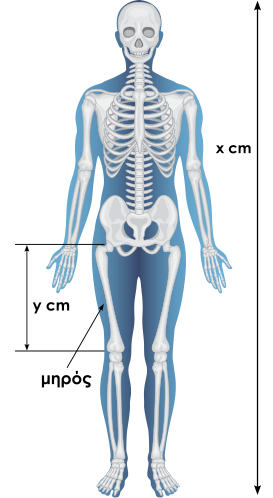
\includegraphics[height=7cm]{32753}
\captionof{figure}{Άσκηση 32753}}{
Οι ανθρωπολόγοι για να προσεγγίσουν το ύψος ενός ενήλικα, χρησιμοποιούν τις παρακάτω εξισώσεις που παριστάνουν τη σχέση μεταξύ του μήκους $y$ (σε cm) οστού του μηρού και του ύψους $x$ (σε cm) του ενήλικα ανάλογα με το φύλο του:

Γυναίκα: $x = 2{,}47y + 54{,}10$

Άνδρας: $x = 2{,}32y + 65{,}53$

\begin{alist}
\item Ένας ανθρωπολόγος ανακαλύπτει ένα μηριαίο οστό μήκους $45{,}5$ cm που ανήκει σε γυναίκα. Να υπολογίσετε το ύψος της γυναίκας.
\monades{8}
\item Ο ανθρωπολόγος βρίσκει μεμονωμένα οστά χεριού, τα οποία εκτιμά ότι ανήκουν σε άντρα ύψους περίπου $171$ cm. Λίγα μέτρα πιο κάτω, ανακαλύπτει ένα μηριαίο οστό μήκους $45{,}5$ cm που ανήκει σε άντρα. Είναι πιθανόν το μηριαίο οστό και τα οστά χεριού να προέρχονται από το ίδιο άτομο; Να αιτιολογήσετε την απάντησή σας.
\monades{8}
\item Να εξετάσετε αν μπορεί ένας άνδρας και μια γυναίκα ίδιου ύψους να έχουν μηριαίο οστό ίδιου μήκους.
\monades{9}
\end{alist}}


\Askhsh{33579}{4}
\begin{ylh}{2}
    \item 3.3. Εξισώσεις 2ου Βαθμού
    \item 5.2. Αριθμητική πρόοδος
\end{ylh}
Οι αριθμοί: $x^2+5, x^2+x, 2x+4$, με τη σειρά που δίνονται, είναι διαδοχικοί όροι αριθμητικής προόδου.

\begin{alist}
\item Να βρείτε τις δυνατές τιμές του αριθμού $x$.
\monades{6}
\item Αν $x=1$ και ο αριθμός $a_4$ είναι ο 4\textsuperscript{ος} όρος της προόδου, να βρείτε:

\begin{rlist}
\item Τη διαφορά $\omega$ της αριθμητικής προόδου.
\monades{5}
\item Τον πρώτο όρο της προόδου.
\monades{6}
\item Το άθροισμα $S_{10}$.
\monades{8}
\end{rlist}
\end{alist}


% --- Άσκηση 33581 (33581.tex) ---
\Askhsh{33581}{4}
\begin{ylh}{2}
    \item 5.2. Αριθμητική πρόοδος
\end{ylh}
Σε μια αριθμητική πρόοδος $(a_\nu)$, ο 3\textsuperscript{ος} όρος είναι $a_3 = 20$ και ο 8\textsuperscript{ος} όρος είναι $a_8 = 50$.

\begin{alist}
\item Να βρείτε τον 1\textsuperscript{ο} όρο $a_1$ και τη διαφορά $\omega$ της προόδου.
\monades{9}
Αν $a_1 = 8$ και $\omega = 6$,

\item Να υπολογίσετε τον 31\textsuperscript{ο} όρο της προόδου.
\monades{6}
\item Να υπολογίσετε το άθροισμα: $S = a_{31} + a_{32} + \dots + a_{40}$
\monades{10}
\end{alist}

% --- Άσκηση 33582 (33582.tex) ---
\Askhsh{33582}{4}
\begin{ylh}{2}
    \item 3.3. Εξισώσεις 2ου Βαθμού
    \item 4.1. Ανισώσεις 1ου Βαθμού
    \item 4.2. Ανισώσεις 2ου Βαθμού
\end{ylh}
Ένα ορθογώνιο έχει περίμετρο $P = 80$. Αν $x$ είναι το μήκος του ορθογωνίου, τότε να δείξετε ότι:

\begin{alist}
\item $0 < x < 40$.
\monades{4}
\item Το εμβαδόν $E(x)$ του ορθογωνίου δίνεται από τη σχέση $E(x) = 40x - x^2$.
\monades{8}
\item Για το εμβαδόν $E(x)$ του ορθογωνίου ισχύει: $E(x) \le 400$, για κάθε $x \in (0, 40)$.
\monades{6}
\item Από όλα τα ορθογώνια με σταθερή περίμετρο $P = 80$, εκείνο που έχει το μεγαλύτερο εμβαδόν είναι το τετράγωνο πλευράς $x = 20$.
\monades{7}
\end{alist}

\Askhsh{33583}{4}
\begin{ylh}{2}
    \item 5.2. Αριθμητική πρόοδος
\end{ylh}
Δίνεται αριθμητική πρόοδος $(a_\nu)$ με $a_1 = 2$ και $a_{10} = 29$.

\begin{alist}
\item Να αποδείξετε ότι ο πρώτος όρος της προόδου είναι $a_1 = 2$ και η διαφορά είναι $\omega = 3$.
\monades{8}
\item Να εξετάσετε αν ο αριθμός $101$ είναι όρος της προόδου.
\monades{8}
\item Να εξετάσετε αν υπάρχουν διαδοχικοί όροι $a_\kappa$ και $a_\lambda$ της παραπάνω προόδου $(a_\nu)$, τέτοιοι ώστε να ισχύει: $\dfrac{a_\kappa}{2} = \dfrac{a_\lambda}{3}$.
\monades{9}
\end{alist}


\Askhsh{33584}{4}
\begin{ylh}{2}
    \item 2.3. Απόλυτη Τιμή Πραγματικού Αριθμού
    \item 3.1. Εξισώσεις 1ου Βαθμού
    \item 3.3. Εξισώσεις 2ου Βαθμού
\end{ylh}
Δίνεται η εξίσωση: $x^2 - (\lambda-1)x + \lambda + 5 = 0$, με παράμετρο $\lambda \in \mathbb{R}$.

\begin{alist}
\item Να αποδείξετε ότι η εξίσωση έχει δύο ρίζες $x_1, x_2$ διαφορετικές μεταξύ τους.
\monades{6}
\item Να δείξετε ότι: $d = |x_1-x_2|$. \monades{4}
\item Αν για τις ρίζες $x_1, x_2$ ισχύει επιπλέον $d = 2$, τότε:
\begin{rlist}
\item
  Να δείξετε ότι: $(\lambda+3)(\lambda+7) = 0$. \monades{7}
\item
  Να βρείτε τις ρίζες $x_1, x_2$ και την τιμή του $\lambda$. \monades{8}
\end{rlist}
\end{alist}


% --- Άσκηση 33585 (33585.tex) ---
\Askhsh{33585}{4}
\begin{ylh}{2}
    \item 2.3. Απόλυτη Τιμή Πραγματικού Αριθμού
    \item 3.3. Εξισώσεις 2ου Βαθμού
\end{ylh}
Δίνεται η εξίσωση $a x^2 - (a^2 - 1)x - a = 0$, με παράμετρο $a \neq 0$.

\begin{alist}
\item Να αποδείξετε ότι η διακρίνουσα της εξίσωσης είναι: $\Delta = (a^2 + 1)^2$. \monades{5}
\item Να βρείτε τις ρίζες $\rho_1$ και $\rho_2$ της εξίσωσης, ως συνάρτηση του $a$. \monades{10}
Αν οι ρίζες της εξίσωσης είναι $\rho_1 = a$ και $\rho_2 = -1/a$,

\item Να βρείτε τις τιμές του $a$ ώστε $|\rho_1 - \rho_2| = 2$. \monades{10}\monades{10}
\end{alist}

% --- Άσκηση 33586 (33586.tex) ---
\Askhsh{33586}{4}
\begin{ylh}{2}
    \item 4.1. Ανισώσεις 1ου Βαθμού
\end{ylh}
Δύο φίλοι αποφασίζουν να συνεταιριστούν και ανοίγουν μια επιχείρηση που γεμίζει τόνερ (toner) για φωτοτυπικά μηχανήματα.

Τα πάγια μηνιαία έξοδα της εταιρείας ανέρχονται στο ποσό των $1200$ ευρώ (για ενοίκιο, παροχές, μισθούς, φόρους, κ.α.).

Το κόστος γεμίσματος ενός τόνερ είναι $10$ ευρώ, η δε τιμή πώλησης του ενός τόνερ καθορίζεται σε $25$ ευρώ.

\begin{alist}
\item Να γράψετε μια σχέση που να περιγράφει το μηναίο κόστος $K(\nu)$ της επιχείρησης, εάν γεμίζει $\nu$ τόνερ το μήνα.
\monades{5}
\item Να γράψετε μια σχέση που να περιγράφει τα μηναία έσοδα $E(\nu)$ της επιχείρησης από την πώληση $\nu$ τόνερ το μήνα.
\monades{5}
\item Να βρείτε πόσα τόνερ πρέπει να πωλούνται κάθε μήνα ώστε η επιχείρηση

\begin{rlist}
\item να μην έχει ζημιά.
\monades{7}
\item να έχει μηνιαίο κέρδος τουλάχιστον $500$ ευρώ.
\monades{8}
\end{rlist}
\end{alist}

% --- Άσκηση 33587 (33587.tex) ---
\Askhsh{33587}{4}
\begin{ylh}{2}
    \item 2.3. Απόλυτη Τιμή Πραγματικού Αριθμού
    \item 3.3. Εξισώσεις 2ου Βαθμού
    \item 4.2. Ανισώσεις 2ου Βαθμού
\end{ylh}
Δίνεται το τριώνυμο $f(x) = -x^2 + 2x + 3, x \in \mathbb{R}$.

\begin{alist}
\item Να βρείτε το πρόσημο του παραπάνω τριωνύμου για τις διάφορες τιμές του $x \in \mathbb{R}$. \monades{9}
\item Να βρείτε, αιτιολογώντας την απάντησή σας, το πρόσημο του γινομένου: $f(2,999) \cdot f(-1,002)$. \monades{7}
\item Αν $-3 < a < 3$, να βρείτε το πρόσημο του αριθμού $-a^2 + 2a + 3$. \monades{9}\monades{9}
\end{alist}

% --- Άσκηση 33597 (33597.tex) ---
\Askhsh{33597}{4}
\begin{ylh}{2}
    \item 2.3. Απόλυτη Τιμή Πραγματικού Αριθμού
    \item 3.1. Εξισώσεις 1ου Βαθμού
    \item 4.1. Ανισώσεις 1ου Βαθμού
    \item 6.2. Γραφική Παράσταση Συνάρτησης
\end{ylh}

Στο παρακάτω σχήμα δίνονται οι γραφικές παραστάσεις $C_f$ και $C_g$ των συναρτήσεων $f(x) = |x-2|$ και $g(x) = -x + 4$ αντίστοιχα, με $x \in \mathbb{R}$.

\begin{center}
\begin{tikzpicture}
\begin{axis}[
    axis lines = middle,
    xlabel = {$x$},
    ylabel = {$y$},
    xmin = -4, xmax = 9,
    ymin = -1, ymax = 6,
    xtick = {-3,-2,-1,1,2,3,4,5,6,7,8},
    ytick = {1,2,3,4,5},
    grid = both,
    grid style = {gray!30},
    width = 12cm, height = 8cm,
    tick label style = {font=\small},
    every axis x label/.style = {at={(current axis.right of origin)}, anchor=north west},
    every axis y label/.style = {at={(current axis.above origin)}, anchor=south east},
]

% --- Άσκηση 33698 (33698.tex) ---
\Askhsh{33698}{4}
\begin{ylh}{2}
    \item 3.3. Εξισώσεις 2ου Βαθμού
    \item 4.2. Ανισώσεις 2ου Βαθμού
\end{ylh}
Δίνεται το τριώνυμο $f(x) = x^{2} - 6x + \lambda - 3$, με $\lambda\mathbb{\in R\ .}$

\begin{alist}
\item Να υπολογίσετε την διακρίνουσα $\Delta$ του τριωνύμου.
\monades{5}
\item Να βρείτε τις τιμές του $\lambda$ για τις οποίες το τριώνυμο έχει δύο άνισες πραγματικές ρίζες.
\monades{7}
\item Αν $3 < \lambda < 12$ τότε:


\begin{rlist}
\item
  Να δείξετε ότι το τριώνυμο έχει δύο άνισες θετικές ρίζες.
\monades{6}
\item
  Αν $x_{1},x_{2}$ με $x_{1} < x_{2}$ είναι οι δύο ρίζες του τριωνύμου και $\kappa$, $\mu$ είναι δύο αριθμοί με $\kappa < 0$ και $x_{1} < \mu < x_{2}$, να προσδιορίσετε το πρόσημο του γινομένου\\
  $\kappa \cdot f(\kappa)\text{⋅}\mu \cdot f(\mu)$. Να αιτιολογήσετε την απάντησή σας
\monades{7}
\end{rlist}
\end{alist}

\Askhsh{33701}{4}
\begin{ylh}{2}
    \item 2.3. Απόλυτη Τιμή Πραγματικού Αριθμού
    \item 3.3. Εξισώσεις 2ου Βαθμού
    \item 4.2. Ανισώσεις 2ου Βαθμού
    \item 6.1. Η Έννοια της Συνάρτησης
    \item 6.2. Γραφική Παράσταση Συνάρτησης
\end{ylh}
Δίνονται οι συναρτήσεις $f(x) = (x - 1)^{2} - 4$ και $g(x) = |x - 1| + 2$ με $x\mathbb{\in R\ .}$

\begin{alist}
\item Να βρείτε τις τιμές του $x$ για τις οποίες η γραφική παράσταση της συνάρτησης $f$ βρίσκεται πάνω από τον άξονα $x'x$.
\monades{9}
\item Να δείξετε ότι για κάθε τιμή του $x$ η γραφική παράσταση της συνάρτησης $g$ βρίσκεται πάνω από τον άξονα $x'x$.
\monades{4}
\item Να βρείτε τα κοινά σημεία των γραφικών παραστάσεων των συναρτήσεων $f$ και $g$.
\monades{12}
\end{alist}


\Askhsh{33711}{4}
\begin{ylh}{2}
    \item 2.3. Απόλυτη Τιμή Πραγματικού Αριθμού
    \item 4.2. Ανισώσεις 2ου Βαθμού
\end{ylh}
Δίνεται το τριώνυμο:
\begin{equation*}x^{2} - 2x - 8.\end{equation*}
\begin{alist}
\item Να βρείτε το πρόσημο του τριωνύμου για τις διάφορες τιμές του πραγματικού αριθμού $x$.
\monades{10}
\item Αν $\kappa = - \dfrac{8889}{4444}$, η τιμή της παράστασης $\kappa^{2} - 2\kappa - 8$ είναι μηδέν, θετικός ή αρνητικός αριθμός; Να αιτιολογήσετε την απάντησή σας.
\monades{8}
\item Αν ισχύει $- 4 < \mu < 4$, ποιο είναι το πρόσημο της τιμής της παράστασης:

\begin{equation*}\mu^{2} - 2|\mu| - 8;\end{equation*}

Να αιτιολογήσετε την απάντησή σας.
\monades{7}
\end{alist}


\Askhsh{33712}{4}
\begin{ylh}{2}
    \item 4.2. Ανισώσεις 2ου Βαθμού
\end{ylh}
Δίνεται το τριώνυμο: $x^{2} + \beta x + \beta^{2}$, όπου $\beta\mathbb{\in \mathbb{R}}$.
\begin{alist}
\item Να υπολογίσετε τη διακρίνουσα $\Delta$ του τριωνύμου.
\monades{4}
\item
\begin{rlist}
\item
  Αν $\beta \neq 0$, τι μπορείτε να πείτε για το πρόσημο του τριωνύμου;
\monades{7}
\item
  Πως αλλάζει η απάντησή σας στο ερώτημα (i), όταν $\beta = 0$;
\monades{6}
\item Με τη βοήθεια της απάντησης στο ερώτημα β), να αποδείξετε ότι ισχύει η ανισότητα
\begin{equation*}
a^{2} + a\beta + \beta^{2} > 0
\end{equation*}
για οποιουσδήποτε πραγματικούς αριθμούς $a,\ \beta$ που δεν είναι και οι δύο ταυτόχρονα $0$.
\monades{8}
\end{rlist}
\end{alist}


\Askhsh{33754}{4}
\begin{ylh}{2}
    \item 3.1. Εξισώσεις 1ου Βαθμού
    \item 6.1. Η Έννοια της Συνάρτησης
    \item 6.2. Γραφική Παράσταση Συνάρτησης
\end{ylh}
Για την ενοικίαση ενός συγκεκριμένου τύπου αυτοκινήτου για μια ημέρα, η εταιρία Α χρεώνει τους πελάτες της σύμφωνα με τον τύπο:
\begin{equation*}y = 60 + 0,20x\end{equation*}

Όπου $x$ είναι η απόσταση που διανύθηκε σε km και $y$ το ποσό της χρέωσης σε ευρώ.

\begin{alist}
\item Τι ποσό θα πληρώσει ένας πελάτης της εταιρείας Α ο οποίος, σε μια ημέρα, ταξίδεψε $400Km$;
\monades{5}
\item Πόσα χιλιόμετρα ταξίδεψε ένας πελάτης ο οποίος για μια ημέρα πλήρωσε $150$ ευρώ;
\monades{5}
\item Μια άλλη εταιρεία, η Β, χρεώνει τους πελάτες της ανά ημέρα σύμφωνα με τον τύπο:

\begin{equation*}y = 80 + 0,10x\end{equation*}

όπου, όπως και προηγουμένως, $x$ είναι η απόσταση που διανύθηκε σε km και $y$ είναι το ποσό της χρέωσης σε ευρώ. Να εξετάσετε ποια από τις δύο εταιρείες μας συμφέρει να επιλέξουμε, ανάλογα με την απόσταση που σκοπεύουμε να διανύσουμε.
\monades{10}
\item Αν $f(x) = 60 + 0,20x$ και $g(x) = 0,80 + 0,10x$ είναι οι συναρτήσεις που εκφράζουν τον τρόπο χρέωσης των εταιρειών Α κα Β αντίστοιχα, να βρείτε τις συντεταγμένες του σημείου τομής των γραφικών παραστάσεων των συναρτήσεων $f$ και $g$ και να εξηγήσετε τι εκφράζει η τιμή κάθε μιας από τις συντεταγμένες σε σχέση με το πρόβλημα το ερωτήματος γ).

\monades{5}
\end{alist}


% --- Άσκηση 33826 (33826.tex) ---
\Askhsh{33826}{4}
\begin{ylh}{2}
    \item 2.3. Απόλυτη Τιμή Πραγματικού Αριθμού
    \item 3.3. Εξισώσεις 2ου Βαθμού
\end{ylh}

\begin{alist}
\item Δίνεται η εξίσωση:

\begin{equation*}x^{4} - 8x^{2} - 9 = 0.\end{equation*}

Να δείξετε ότι η εξίσωση αυτή έχει δύο μόνο πραγματικές ρίζες, τις οποίες και να προσδιορίσετε.
\monades{10}
\item Γενικεύοντας το παράδειγμα του προηγούμενου ερωτήματος, θεωρούμε την εξίσωση:
$x^{4} + \beta x^{2} + \gamma = 0$ (1) με παραμέτρους $\beta,\gamma \in \mathbb{R}$. Να δείξετε ότι αν $\gamma < 0$, τότε:
\begin{rlist}
\item
  $\beta^{2} - 4\gamma > 0$.
\monades{3}
\item
  Η εξίσωση (1) έχει δύο μόνο διαφορετικές πραγματικές ρίζες.
\monades{12}
\end{rlist}
\end{alist}

% --- Άσκηση 33855 (33855.tex) ---
\Askhsh{33855}{4}
\begin{ylh}{2}
    \item 3.3. Εξισώσεις 2ου Βαθμού
    \item 4.2. Ανισώσεις 2ου Βαθμού
\end{ylh}

\begin{alist}
\item Θεωρούμε την εξίσωση $x^{2} + 2x + 3 = a$, με παράμετρο $a\mathbb{\in R}$.
\begin{rlist}
\item Να βρείτε για ποιες τιμές του $a$ η εξίσωση $x^{2} + 2x + 3 = a$ έχει δύο πραγματικές και άνισες ρίζες.
\monades{6}
\item Να βρείτε την τιμή του $a$ ώστε η εξίσωση να έχει μια διπλή ρίζα, την οποία και να προσδιορίσετε.
\monades{6}
\end{rlist}
\item Δίνεται η συνάρτηση $f(x) = x^{2} + 2x + 3$, $x\mathbb{\in R}$.
\begin{alist}
\item Να αποδείξετε ότι $f(x) \geq 2$ για κάθε $x\mathbb{\in R}$.
\monades{7}
\item Να λύσετε την ανίσωση $\sqrt{f(x) - 2} \leq 2$.
\monades{6}
\end{alist}
\end{alist}

% --- Άσκηση 33858 (33858.tex) ---
\Askhsh{33858}{4}
\begin{ylh}{2}
    \item 3.3. Εξισώσεις 2ου Βαθμού
    \item 5.2. Αριθμητική πρόοδος
\end{ylh}
Σε αριθμητική πρόοδο $\left( a_{\nu} \right)$ είναι $a_{2} = \kappa^{2}$ και $a_{3} = (\kappa + 1)^{2}$, όπου $\kappa$ ακέραιος με $\kappa > 1$.

\begin{alist}
\item Να αποδείξετε ότι η διαφορά $\omega$ της προόδου είναι περιττός αριθμός.
\monades{8}
\item Αν επιπλέον ο πρώτος όρος της είναι $a_{1} = 2$, τότε:
\begin{rlist}
\item
  Να βρείτε την τιμή του $\kappa$ και να αποδείξετε ότι$\ \omega = 7$.
\monades{8}
\item
  Να εξετάσετε αν ο αριθμός $72$ είναι όρος της προόδου.
\monades{9}
\end{rlist}
\end{alist}

% --- Άσκηση 33888 (33888.tex) ---
\Askhsh{33888}{4}
\begin{ylh}{2}
    \item 2.2. Διάταξη Πραγματικών Αριθμών
    \item 2.3. Απόλυτη Τιμή Πραγματικού Αριθμού
\end{ylh}
Δίνονται οι πραγματικοί αριθμοί $a$ και $\beta$ για τους οποίους ισχύει:
$(a - 1)(1 - \beta) > 0$
\begin{alist}
\item Να δείξετε ότι το 1 είναι μεταξύ των $a$ και $\beta$.
\monades{13}
\item Αν επιπλέον $\beta - a = 4$, να υπολογίσετε την τιμή της παράστασης

$K = |a - 1| + |1 - \beta|$.
\monades{12}
\end{alist}

\Askhsh{33889}{4}
\begin{ylh}{2}
    \item 3.3. Εξισώσεις 2ου Βαθμού
\end{ylh}

\begin{alist}
\item Να λύσετε τις εξισώσεις $3x^2 - 14x + 8 = 0$ (1) και $8x^2 - 14x + 3 = 0$ (2). \monades{10}
\item Ένας μαθητής παρατήρησε ότι οι ρίζες της εξίσωσης (2) είναι οι αντίστροφοι των ριζών της εξίσωσης (1) και ισχυρίστηκε ότι το ίδιο θα ισχύει για οποιοδήποτε ζευγάρι εξισώσεων της μορφής: $a x^2 + \beta x + \gamma = 0$ (3) και $\gamma x^2 + \beta x + a = 0$ (4), με $a \cdot \gamma \neq 0$.

 Να αποδείξετε τον ισχυρισμό του μαθητή, δείχνοντας ότι: Αν ο αριθμός $\rho$ είναι ρίζα της εξίσωσης (3) και $a \cdot \gamma \neq 0$, τότε:

\begin{rlist}
\item $\rho \neq 0$. \monades{5}
\item $\dfrac{1}{\rho}$ είναι ρίζα της εξίσωσης (4). \monades{10}
\end{rlist}
\end{alist}


% --- Άσκηση 33890 (33890.tex) ---
\Askhsh{33890}{4}
\begin{ylh}{2}
    \item 2.2. Διάταξη Πραγματικών Αριθμών
    \item 4.2. Ανισώσεις 2ου Βαθμού
\end{ylh}

\begin{alist}
\item Να λύσετε την ανίσωση $x^2 + 1 \ge \dfrac{5}{2}x$ (1). \monades{10}
\item Δίνονται δύο αριθμοί $\kappa, \lambda$ οι οποίοι είναι λύσεις της ανίσωσης (1) και ικανοποιούν επιπλέον τη σχέση $(\lambda - 1)(\kappa - 1) < 0$.

\begin{rlist}
\item Να δείξετε ότι το 1 είναι μεταξύ των αριθμών $\kappa, \lambda$. \monades{8}
\item Να δείξετε ότι $|\kappa - \lambda| \ge \dfrac{3}{2}$. \monades{7}
\end{rlist}
\end{alist}

% --- Άσκηση 33891 (33891.tex) ---
\Askhsh{33891}{4}
\begin{ylh}{2}
    \item 5.3. Γεωμετρική πρόοδος
\end{ylh}
Δίνεται η γεωμετρική πρόοδος $(a_\nu)$ με λόγο $\lambda$ για την οποία ισχύουν: $a_3 = 4, a_5 = 16$ και $\lambda > 0$.

\begin{alist}
\item Να βρείτε τον πρώτο όρο $a_1$ και τον λόγο $\lambda$ της προόδου. \monades{8}
\item Να αποδείξετε ότι η ακολουθία $(\beta_\nu)$, με $\beta_\nu = 1/a_\nu, \nu = 1, 2, 3, \dots$ είναι επίσης γεωμετρική πρόοδος με λόγο τον αντίστροφο του λόγου της $(a_\nu)$. \monades{9}
\item Αν $S_{10}$ είναι το άθροισμα των 10 πρώτων όρων της $(a_\nu)$ και $S'_{10}$ το άθροισμα των 10 πρώτων όρων της $(\beta_\nu)$ αντίστοιχα, να δείξετε ότι ισχύει η σχέση: $S'_{10} = \dfrac{1}{2^9} S_{10}$. \monades{8}
\end{alist}

\Askhsh{33892}{4}
\begin{ylh}{2}
    \item 2.2. Διάταξη Πραγματικών Αριθμών
    \item 2.3. Απόλυτη Τιμή Πραγματικού Αριθμού
    \item 4.1. Ανισώσεις 1ου Βαθμού
    \item 4.2. Ανισώσεις 2ου Βαθμού
\end{ylh}

\begin{alist}
\item Να λύσετε την ανίσωση $x^2 + x - 2 \leq 0$.
\monades{8}
\item Να λύσετε την ανίσωση $|x^2 + x - 2| \leq 2 - x - x^2$.\monades{5}
\item Δίνεται το παρακάτω ορθογώνιο με πλευρές $a$ και $a + 1$. Ο αριθμός $a$ ικανοποιεί τη σχέση $a^2 + a - 2 \leq 0$. Αν για το εμβαδόν $E$ του ορθογωνίου ισχύει $E = a(a + 1)$, τότε:
\begin{center}
\begin{tikzpicture}[scale=0.5]
    % Ορθογώνιο α × (α+1)
    \draw[l4, maincolor!70!black,fill=maincolor!20] (0,0) rectangle (8,5);
    \fill[maincolor!5] (0,0) rectangle (8,5);
    % Ετικέτες
    \node[left] at (0,2.5) {$a$};
    \node[below] at (4,0) {$a + 1$};
\end{tikzpicture}\captionof{figure}{Άσκηση 33892}
\end{center}
\begin{rlist}
\item Να δείξετε ότι $0 < E \leq 2$.
\monades{7}
\item Να βρείτε μεταξύ ποιων αριθμών κυμαίνεται η περίμετρος του ορθογωνίου.
\monades{5}
\end{rlist}
\end{alist}


\Askhsh{33893}{4}
\begin{ylh}{2}
    \item 2.2. Διάταξη Πραγματικών Αριθμών
    \item 2.3. Απόλυτη Τιμή Πραγματικού Αριθμού
    \item 4.1. Ανισώσεις 1ου Βαθμού
\end{ylh}

\begin{alist}
\item Να βρείτε τους πραγματικούς αριθμούς $x$ για τους οποίους ισχύει $|x - 4| < 2$. \monades{7}
\item Θεωρούμε πραγματικό αριθμό $x$ του οποίου η απόσταση από το 4 πάνω στο άξονα των πραγματικών είναι μικρότερη από 2.

\end{alist}


% --- Άσκηση 33894 (33894.tex) ---
\Askhsh{33894}{4}
\begin{ylh}{2}
    \item 2.3. Απόλυτη Τιμή Πραγματικού Αριθμού
    \item 6.1. Η Έννοια της Συνάρτησης
    \item 6.2. Γραφική Παράσταση Συνάρτησης
    \item 6.3. Η Συνάρτηση $f(x)=ax+\beta$
\end{ylh}
Δίνεται η συνάρτηση $f(x) = \dfrac{x^2 - 5x + 6}{2 - x}$.
\begin{alist}
\item Να βρείτε το πεδίο ορισμού της $f$. \monades{5}
\item Να αποδείξετε ότι $f(x) = \begin{cases} x - 3, & x > 2 \\ -x + 3, & x < 2 \end{cases}$. \monades{7}
\begin{rlist}
\item Να χαράξετε τη γραφική παράσταση της $f$. \monades{4}
\item Να βρείτε τα σημεία τομής της γραφικής παράστασης της $f$ με τους άξονες $x'x$ και $y'y$. \monades{4}
\end{rlist}
\item Να λύσετε την ανίσωση $f(x) \le 0$. \monades{5}
\end{alist}

% --- Άσκηση 33895 (33895.tex) ---
\Askhsh{33895}{4}
\begin{ylh}{2}
    \item 6.1. Η Έννοια της Συνάρτησης
    \item 6.2. Γραφική Παράσταση Συνάρτησης
    \item 6.3. Η Συνάρτηση $f(x)=ax+\beta$
\end{ylh}
Δίνεται η συνάρτηση $f(x) = \dfrac{4x^2 - 2(a + 3)x + 3a}{2x - 3}$, με παράμετρο $a \in \mathbb{R}$.

\begin{alist}
\item Να βρείτε το πεδίο ορισμού της $f$. \monades{5}
\item Να αποδείξετε ότι $f(x) = 2x - a$, για κάθε $x$ που ανήκει στο πεδίο ορισμού της $f$. \monades{8}
\item Να βρείτε την τιμή του $a \in \mathbb{R}$, αν η γραφική παράσταση της $f$ διέρχεται από το σημείο $(1, -1)$. \monades{7}
\item Να βρείτε, αν υπάρχουν, τα σημεία τομής της γραφικής παράστασης της $f$ με τους άξονες $x'x$ και $y'y$. \monades{5}
\end{alist}

\Askhsh{33896}{4}
\begin{ylh}{2}
    \item 2.2. Διάταξη Πραγματικών Αριθμών
    \item 2.3. Απόλυτη Τιμή Πραγματικού Αριθμού
    \item 4.1. Ανισώσεις 1ου Βαθμού
\end{ylh}
Για τους πραγματικούς αριθμούς $a, \beta \in \mathbb{R}$ ισχύει ότι: $|a - 2| < 1$ και $|\beta - 3| \le 2$.

\begin{alist}
\item Να αποδείξετε ότι $1 < a < 3$. \monades{4}
\item Να βρείτε τα όρια μεταξύ των οποίων βρίσκεται ο $\beta$. \monades{5}
\item Να βρείτε μεταξύ ποιων τιμών κυμαίνεται η τιμή της παράστασης $2a - 3\beta$. \monades{7}
\item Να βρείτε μεταξύ ποιων τιμών κυμαίνεται η τιμή της παράστασης $a/\beta$. \monades{9}
\end{alist}


\Askhsh{34145}{2}
\begin{ylh}{2}
    \item 5.2. Αριθμητική πρόοδος
\end{ylh}
Δίνεται αριθμητική πρόοδος $(a_\nu)$ με διαφορά $\omega$.
\begin{alist}
\item Να δείξετε ότι: $\dfrac{a_{15} - a_9}{a_{10} - a_7} = 2$. \monades{13}
\item Αν $a_{15} - a_9 = 18$, να βρείτε τη διαφορά $\omega$ της προόδου. \monades{12}
\end{alist}


\Askhsh{34146}{2}
\begin{ylh}{2}
    \item 3.1. Εξισώσεις 1ου Βαθμού
\end{ylh}
Δίνεται η εξίσωση: $(a + 3)x = a^2 - 9$, με παράμετρο $a \in \mathbb{R}$.
\begin{alist}
\item Να λύσετε την εξίσωση στις παρακάτω περιπτώσεις:
\begin{rlist}
\item Όταν $a = 1$. \monades{5}
\item Όταν $a = -3$. \monades{8}
\end{rlist}
\item Να βρείτε τις τιμές του $a$, για τις οποίες η εξίσωση έχει μοναδική λύση και να προσδιορίσετε τη λύση αυτή. \monades{12}
\end{alist}


\Askhsh{34147}{2}
\begin{ylh}{2}
    \item 5.2. Αριθμητική πρόοδος
\end{ylh}
Σε αριθμητική πρόοδο $(a_\nu)$ με διαφορά $\omega = 4$, ισχύει: $a_6 + a_{11} = 40$.

\begin{alist}
\item Να βρείτε τον πρώτο όρο $a_1$ της προόδου. \monades{12}
\item Πόσους πρώτους όρους της προόδου πρέπει να προσθέσουμε ώστε το άθροισμά τους να είναι ίσο με το μηδέν; Να αιτιολογήσετε την απάντησή σας. \monades{13}
\end{alist}


% --- Άσκηση 34148 (34148.tex) ---
\Askhsh{34148}{2}
\begin{ylh}{2}
    \item 2.3. Απόλυτη Τιμή Πραγματικού Αριθμού
    \item 4.1. Ανισώσεις 1ου Βαθμού
\end{ylh}

\begin{rlist}
\item Να λύσετε τις ανισώσεις και να παραστήσετε τις λύσεις τους στον άξονα των πραγματικών αριθμών:
\begin{multicols}{2}
\begin{alist}
\item $|2x - 3| \le 5$ \monades{9}
\item $|2x - 3| \ge 1$ \monades{9}
\end{alist}
\end{multicols}
\item Να βρείτε τις τιμές του $x$ για τις οποίες συναληθεύουν οι παραπάνω ανισώσεις. \monades{7}
\end{rlist}

\Askhsh{34149}{2}
\begin{ylh}{2}
    \item 2.3. Απόλυτη Τιμή Πραγματικού Αριθμού
    \item 3.3. Εξισώσεις 2ου Βαθμού
\end{ylh}

\begin{alist}
\item Να λύσετε την εξίσωση: $2x^2 - x - 6 = 0$ (1). \monades{9}
\item Να λύσετε την ανίσωση: $|x - 1| < 2$ (2). \monades{9}
\item Να εξετάσετε αν υπάρχουν τιμές του $x$ που ικανοποιούν ταυτόχρονα τις (1) και (2). \monades{7}
\end{alist}


% --- Άσκηση 34150 (34150.tex) ---
\Askhsh{34150}{2}
\begin{ylh}{2}
    \item 3.3. Εξισώσεις 2ου Βαθμού
\end{ylh}
Δίνονται δύο πραγματικοί αριθμοί $a, \beta$ τέτοιοι, ώστε: $a + \beta = 12$ και $a^2 + \beta^2 = 272$.
\begin{alist}
\item Με τη βοήθεια της ταυτότητας $(a + \beta)^2 = a^2 + 2a\beta + \beta^2$, να δείξετε ότι: $a \cdot \beta = -64$. \monades{8}
\item Να κατασκευάσετε μια εξίσωση 2\textsuperscript{ου} βαθμού που έχει ρίζες τους αριθμούς $a, \beta$. \monades{10}
\item Να προσδιορίσετε τους αριθμούς $a$ και $\beta$. \monades{7}
\end{alist}

% --- Άσκηση 34152 (34152.tex) ---
\Askhsh{34152}{2}
\begin{ylh}{2}
    \item 2.3. Απόλυτη Τιμή Πραγματικού Αριθμού
    \item 2.4. Ρίζες Πραγματικών Αριθμών
\end{ylh}
Δίνονται οι παραστάσεις: $A = \sqrt{(x - 2)^2}$ και $B = \sqrt[3]{(2 - x)^3}$, όπου $x$ πραγματικός αριθμός.

\begin{alist}
\item Για ποιες τιμές του $x$ ορίζεται η παράσταση $A$; \monades{7}
\item Για ποιες τιμές του $x$ ορίζεται η παράσταση $B$; \monades{8}
\item Να δείξετε ότι, για κάθε $x \le 2$, ισχύει $A = B$. \monades{10}
\end{alist}

\Askhsh{34153}{2}
\begin{ylh}{2}
    \item 5.2. Αριθμητική πρόοδος
\end{ylh}
Οι αριθμοί $x+6, 5x+2, 11x-6$ είναι, με τη σειρά που δίνονται, διαδοχικοί όροι αριθμητικής προόδου με πρώτο όρο $a_1$ και διαφορά $\omega$.

\begin{alist}
\item Να βρείτε την τιμή του $x$ και να αποδείξετε ότι $\omega=4$. \monades{12}
\item Αν ο πρώτος όρος της προόδου είναι $a_1 = 0$, να υπολογίσετε το άθροισμα $S_8$ των 8 πρώτων όρων. \monades{13}
\end{alist}


\Askhsh{34154}{2}
\begin{ylh}{2}
    \item 3.3. Εξισώσεις 2ου Βαθμού
\end{ylh}
Δίνονται οι αριθμοί: $A = \dfrac{1}{3 - \sqrt{7}}$ και $B = \dfrac{1}{3 + \sqrt{7}}$.

\begin{alist}
\item Να δείξετε ότι: $A + B = 3$ και $A \cdot B = 1/2$. \monades{12}
\item Να κατασκευάσετε μια εξίσωση 2{ου} βαθμού που έχει ρίζες τους αριθμούς $A, B$. \monades{13}
\end{alist}


% --- Άσκηση 34155 (34155.tex) ---
\Askhsh{34155}{2}
\begin{ylh}{2}
    \item 2.4. Ρίζες Πραγματικών Αριθμών
\end{ylh}
Αν είναι $A = \sqrt[3]{5}, B = \sqrt{3}, \Gamma = \sqrt[6]{5}$, τότε:
\begin{alist}
\item Να αποδείξετε ότι $A \cdot B \cdot \Gamma = \sqrt{15}$. \monades{15}
\item Να συγκρίνετε τους αριθμούς $A, B$. \monades{10}
\end{alist}

% --- Άσκηση 34156 (34156.tex) ---
\Askhsh{34156}{2}
\begin{ylh}{2}
    \item 5.3. Γεωμετρική πρόοδος
\end{ylh}
Δίνεται η γεωμετρική πρόοδος $(a_\nu)$, για την οποία ισχύει $a_5/a_2 = 27$.

\begin{alist}
\item Να δείξετε ότι ο λόγος της προόδου είναι $\lambda = 3$. \monades{10}
\item Αν το άθροισμα των τεσσάρων πρώτων όρων της προόδου είναι 200, να βρείτε τον πρώτο όρο $a_1$. \monades{15}
\end{alist}

% --- Άσκηση 34157 (34157.tex) ---
\Askhsh{34157}{2}
\begin{ylh}{2}
    \item 2.1. Οι Πράξεις και οι Ιδιότητές τους
    \item 2.4. Ρίζες Πραγματικών Αριθμών
\end{ylh}
Αν είναι $A = 2 - \sqrt{3}, B = 2 + \sqrt{3}$, τότε:
\begin{alist}
\item Να αποδείξετε ότι $A \cdot B = 1$. \monades{12}
\item Να υπολογίσετε την τιμή της παράστασης $\Pi = A^2 + B^2$. \monades{13}
\end{alist}

\Askhsh{34158}{2}
\begin{ylh}{2}
    \item 3.3. Εξισώσεις 2ου Βαθμού
    \item 5.2. Αριθμητική πρόοδος
\end{ylh}
Σε αριθμητική πρόοδο $(a_\nu)$ είναι $a_1 = 2$ και $a_5 = 14$.
\begin{alist}
\item Να αποδείξετε ότι η διαφορά $\omega$ της προόδου είναι ίση με 3.
\monades{12}
\item Να βρείτε πόσους από τους πρώτους όρους της αριθμητικής προόδου $(a_\nu)$ πρέπει να προσθέσουμε, ώστε το άθροισμά τους να είναι ίσο με 77.

(Δίνεται: $\sqrt{1849} = 43$).
\monades{13}
\end{alist}


\Askhsh{34159}{2}
\begin{ylh}{2}
    \item 6.1. Η Έννοια της Συνάρτησης
    \item 6.2. Γραφική Παράσταση Συνάρτησης
\end{ylh}
Δίνεται η συνάρτηση $f$, με $f(x) = \dfrac{x^2 - 5x + 6}{x - 3}$.
\begin{alist}
\item Να βρείτε το πεδίο ορισμού της συνάρτησης $f$. \monades{7}
\item Να απλοποιήσετε τον τύπο της συνάρτησης $f$. \monades{9}
\item Να βρείτε τα σημεία τομής της γραφικής παράστασης της $f$ με τους άξονες $x'x$ και $y'y$. \monades{9}
\end{alist}


\Askhsh{34161}{2}
\begin{ylh}{2}
    \item 2.3. Απόλυτη Τιμή Πραγματικού Αριθμού
    \item 3.1. Εξισώσεις 1ου Βαθμού
    \item 3.3. Εξισώσεις 2ου Βαθμού
\end{ylh}

\begin{alist}
\item Να λύσετε την εξίσωση $|2x - 1| = 3$. \monades{12}
\item Αν $a, \beta$ με $a < \beta$ είναι οι ρίζες της εξίσωσης του ερωτήματος (α), τότε να λύσετε την εξίσωση $a x^2 + \beta x + 3 = 0$. \monades{13}
\end{alist}


\Askhsh{34162}{2}
\begin{ylh}{2}
    \item 4.1. Ανισώσεις 1ου Βαθμού
    \item 4.2. Ανισώσεις 2ου Βαθμού
\end{ylh}

\begin{alist}
\item Να λύσετε την ανίσωση $|2x - 5| \leq 3$. (1)
\monades{7}
\item Να λύσετε την ανίσωση $2x^{2} - x - 1 \geq 0.$ (2)
\monades{9}
\item Να βρείτε τις κοινές λύσεις των ανισώσεων (1) και (2).
\monades{9}
\end{alist}


% --- Άσκηση 34180 (34180.tex) ---
\Askhsh{34180}{4}
\begin{ylh}{2}
    \item 3.3. Εξισώσεις 2ου Βαθμού
    \item 5.2. Αριθμητική πρόοδος
    \item 5.3. Γεωμετρική πρόοδος
\end{ylh}
Δίνονται οι αριθμοί 2, $x$, 8, $x \in \mathbb{R}$.

\begin{alist}
\item Να βρείτε την τιμή του $x$, ώστε οι αριθμοί 2, $x$, 8, με τη σειρά που δίνονται, να αποτελούν διαδοχικούς όρους αριθμητικής προόδου. Ποια είναι η διαφορά $\omega$ αυτής της προόδου; \monades{5}
\item Να βρείτε τον αριθμό $x$, ώστε οι 2, $x$, 8, με τη σειρά που δίνονται, να αποτελούν διαδοχικούς όρους γεωμετρικής προόδου. Ποιος είναι ο λόγος $\lambda$ αυτής της προόδου; \monades{7}
\item Αν $(a_\nu)$ είναι η αριθμητική πρόοδος $2, 5, 8, 11, \dots$ και $(\beta_\nu)$ η γεωμετρική πρόοδος $2, 4, 8, 16, \dots$, τότε να βρείτε:

\begin{rlist}
\item Το άθροισμα $S_\nu$ των $\nu$ πρώτων όρων της $(a_\nu)$. \monades{5}
\item Την τιμή του $\nu$, ώστε για το άθροισμα $S_\nu$ του γi) ερωτήματος να ισχύει: $2 \cdot (S_\nu + 24) = \beta_7$. \monades{8}
\end{rlist}
\end{alist}

\Askhsh{34181}{4}
\begin{ylh}{2}
    \item 3.3. Εξισώσεις 2ου Βαθμού
    \item 5.3. Γεωμετρική πρόοδος
\end{ylh}
Δίνεται ορθογώνιο μήκους $a$, πλάτους $\beta$ και εμβαδού $E$. Οι αριθμοί $a, E, \beta$, με τη σειρά που δίνονται, αποτελούν διαδοχικούς όρους γεωμετρικής προόδου.

\begin{alist}
\item Να υπολογίσετε την τιμή του εμβαδού $E$. \monades{10}
\item Αν $E = 1$ και $a + \beta = 10$,

\begin{rlist}
\item να κατασκευάσετε μια εξίσωση 2{ου} βαθμού με ρίζες $a$ και $\beta$. \monades{5}
\item να βρείτε τις διαστάσεις $a$ και $\beta$ του ορθογωνίου. \monades{10}
\end{rlist}
\end{alist}


% --- Άσκηση 34182 (34182.tex) ---
\Askhsh{34182}{4}
\begin{ylh}{2}
    \item 3.3. Εξισώσεις 2ου Βαθμού
    \item 4.2. Ανισώσεις 2ου Βαθμού
\end{ylh}
\wrapr{-5mm}{12}{4.5cm}{-5mm}{
\begin{tikzpicture}[scale=1.2]

% --- Άσκηση 34183 (34183.tex) ---
\Askhsh{34183}{4}
\begin{ylh}{2}
    \item 6.2. Γραφική Παράσταση Συνάρτησης
    \item 6.3. Η Συνάρτηση $f(x)=ax+\beta$
\end{ylh}
Σε μια πόλη της Ευρώπης μια εταιρεία ταξί με το όνομα «RED» χρεώνει τον πελάτη $1$ ευρώ με την είσοδο στο ταξί και $0,6$ ευρώ για κάθε χιλιόμετρο που διανύει. Μια άλλη εταιρεία ταξί με το όνομα «YELLOW» χρεώνει τον πελάτη $2$ ευρώ με την είσοδο στο ταξί και $0,4$ ευρώ για κάθε χιλιόμετρο που διανύει. Οι παραπάνω τιμές ισχύουν για αποστάσεις μικρότερες από $15$ χιλιόμετρα.

\begin{alist}
\item

\begin{rlist}
\item Αν $f(x)$ είναι το ποσό (σε ευρώ) που χρεώνει η εταιρεία «RED» για μια διαδρομή $x$ χιλιομέτρων, να μεταφέρετε στην κόλα σας και να συμπληρώσετε τον παρακάτω πίνακα.
\begin{center}
 \begin{tblr}{hlines = {1pt,white},
vlines = {0.5pt,white},
column{odd} = {maincolor!40,c},
column{even} = {maincolor!10,c},
column{1} = {maincolor,c,fg={white}}}
 $x$ (km) & 0 & 2 & 8 \\ 
 $f(x)$ (ευρώ) & & & \\ 
 \end{tblr}
\end{center}\monades{3}
\item Αν $g(x)$ είναι το ποσό (σε ευρώ) που χρεώνει η εταιρεία «YELLOW» για μια διαδρομή $x$ χιλιομέτρων, να μεταφέρετε στην κόλα σας και να συμπληρώσετε τον παρακάτω πίνακα.
\begin{center}
 \begin{tblr}{hlines = {1pt,white},
vlines = {0.5pt,white},
column{odd} = {maincolor!40,c},
column{even} = {maincolor!10,c},
column{1} = {maincolor,c,fg={white}}}

 $x$ (km) & & & \\
 $g(x)$ (ευρώ) & 2 & 3,2 & 4,8 \\
 \end{tblr}
\end{center}\monades{3}
\end{rlist}
\item Να βρείτε το πεδίο ορισμού και τον τύπο των συναρτήσεων $f$ και $g$. \monades{8}
\item Να σχεδιάσετε τις γραφικές παραστάσεις των $f, g$ και να βρείτε για ποιες αποστάσεις η επιλογή της εταιρείας «RED» είναι πιο οικονομική, αιτιολογώντας την απάντησή σας. \monades{8}
\item Αν δυο πελάτες $A$ και $B$ μετακινηθούν με την εταιρεία «RED» και ο πελάτης $A$ διανύσει $3$ χιλιόμετρα περισσότερα από τον $B$, να βρείτε πόσα περισσότερα χρήματα θα πληρώσει ο $A$ σε σχέση με τον $B$. \monades{3}
\end{alist}

\Askhsh{34184}{4}
\begin{ylh}{2}
    \item 3.3. Εξισώσεις 2ου Βαθμού
    \item 4.2. Ανισώσεις 2ου Βαθμού
    \item 6.1. Η Έννοια της Συνάρτησης
\end{ylh}
Θεωρούμε ορθογώνιο τρίγωνο $AB\Gamma$ ($\hat{A} = 90^\circ$) με κάθετες πλευρές $AB = x$ και $A\Gamma = y$, έτσι ώστε $x + y = 10$.

\begin{alist}
\item Να εκφράσετε το εμβαδόν $E$ του τριγώνου $AB\Gamma$ ως συνάρτηση του $x$ και να βρείτε το πεδίο ορισμού της συνάρτησης $E(x)$.
\monades{9}
\item Αν το εμβαδόν του τριγώνου είναι $E(x) = \dfrac{1}{2}(-x^2 + 10x)$, να δείξετε ότι $E(x) \le 25/2$, για κάθε $x \in (0, 10)$.

(Μονάδες9)

\item Να βρείτε την τιμή του $x \in (0, 10)$ ώστε το εμβαδόν $E(x)$ να γίνεται μέγιστο, δηλαδή ίσο με $25/2$. Τι παρατηρείτε τότε για το τρίγωνο $AB\Gamma$;
\monades{7}
\end{alist}


\Askhsh{34185}{4}
\begin{ylh}{2}
    \item 2.3. Απόλυτη Τιμή Πραγματικού Αριθμού
    \item 4.2. Ανισώσεις 2ου Βαθμού
\end{ylh}

\begin{alist}
\item Να λύσετε την ανίσωση $x^2 - 5x - 6 < 0$. \monades{9}
\item Να βρείτε το πρόσημο του αριθμού $K = (-46/47)^2 - 5(-46/47) - 6$ αιτιολογώντας την απάντησή σας. \monades{7}
\item Αν $a \in (-1, 6)$, να βρείτε το πρόσημο της παράστασης $\Lambda = a^2 - 5a - 6$ αιτιολογώντας την απάντησή σας. \monades{9}
\end{alist}


% --- Άσκηση 34186 (34186.tex) ---
\Askhsh{34186}{4}
\begin{ylh}{2}
    \item 3.3. Εξισώσεις 2ου Βαθμού
    \item 4.2. Ανισώσεις 2ου Βαθμού
\end{ylh}
Οι πλευρές $x_1$ και $x_2$ ενός ορθογωνίου είναι ρίζες της εξίσωσης $x^2 - 2x + \lambda(2 - \lambda) = 0$, με $\lambda \in (0, 2)$.

\begin{alist}
\item Να βρείτε

\begin{rlist}
\item την περίμετρο $\Pi$ του ορθογωνίου. \monades{6}
\item το εμβαδόν $E$ του ορθογωνίου ως συνάρτηση του $\lambda$. \monades{6}
\end{rlist}
\item Να δείξετε ότι $E \le 1$, για κάθε $\lambda \in (0, 2)$. \monades{7}
\item Να βρείτε την τιμή του $\lambda \in (0, 2)$ για την οποία το εμβαδόν $E$ του ορθογωνίου γίνεται μέγιστο, δηλαδή ίσο με 1. Τι μπορείτε να πείτε τότε για το ορθογώνιο; \monades{6}
\end{alist}

% --- Άσκηση 34309 (34309.tex) ---
\Askhsh{34309}{4}
\begin{ylh}{2}
    \item 3.3. Εξισώσεις 2ου Βαθμού
    \item 4.1. Ανισώσεις 1ου Βαθμού
    \item 6.1. Η Έννοια της Συνάρτησης
    \item 6.2. Γραφική Παράσταση Συνάρτησης
\end{ylh}
Θεωρούμε τις συναρτήσεις:
$f(x) = x^{2} + 1$ και $g(x) = x + a$ με $x\mathbb{\in R}$ και $a\mathbb{\in R}$.
\begin{alist}
\item Για $a = 1$, να προσδιορίσετε τα κοινά σημεία των γραφικών παραστάσεων των συναρτήσεων $f$ και $g$.
\monades{5}
\item Να βρείτε για ποιες τιμές του $a$, οι γραφικές παραστάσεις των συναρτήσεων $f$ και $g$ τέμνονται σε δύο σημεία.
\monades{10}
\item Για $a > 1$, να εξετάσετε αν οι τετμημένες των σημείων τομής των γραφικών παραστάσεων των συναρτήσεων $f$ και $g$ είναι ομόσημες ή ετερόσημες.
\monades{10}
\end{alist}

% --- Άσκηση 34310 (34310.tex) ---
\Askhsh{34310}{4}
\begin{ylh}{2}
    \item 2.3. Απόλυτη Τιμή Πραγματικού Αριθμού
    \item 3.1. Εξισώσεις 1ου Βαθμού
    \item 3.3. Εξισώσεις 2ου Βαθμού
\end{ylh}
Δίνεται η εξίσωση $\lambda x^{2} + (2\lambda - 1)x + \lambda - 1 = 0$, με παράμετρο $\lambda\mathbb{\in R -}\left\{ 0 \right\}$.
\begin{alist}
\item Να δείξετε ότι η διακρίνουσα $\Delta$ της εξίσωσης είναι ανεξάρτητη του $\lambda$, δηλαδή σταθερή.
\monades{8}
\item Να προσδιορίσετε τις ρίζες της εξίσωσης ως συνάρτηση του $\lambda$.
\monades{7}
\item Να βρείτε για ποιες τιμές του $\lambda$ η απόσταση των ριζών της εξίσωσης στον άξονα των πραγματικών αριθμών είναι ίση με $2$ μονάδες.
\monades{10}
\end{alist}

% --- Άσκηση 34312 (34312.tex) ---
\Askhsh{34312}{4}
\begin{ylh}{2}
    \item 2.3. Απόλυτη Τιμή Πραγματικού Αριθμού
    \item 3.1. Εξισώσεις 1ου Βαθμού
    \item 4.1. Ανισώσεις 1ου Βαθμού
    \item 6.1. Η Έννοια της Συνάρτησης
    \item 6.2. Γραφική Παράσταση Συνάρτησης
\end{ylh}
\wrapr{-5mm}{12}{6.7cm}{-5mm}{
\begin{tikzpicture}
\begin{axis}[
    axis lines = middle,
    xlabel = {$x$},
    ylabel = {$y$},
    xmin = -2, xmax = 6,
    ymin = -0.5, ymax = 5,
    xtick = {-1,0,1,2,3,4,5},
    ytick = {1,2,3,4},
    grid = both,
    grid style = {gray!30},
    width = 8cm, height = 7cm,
    tick label style = {font=\small},
    every axis x label/.style = {at={(current axis.right of origin)}, anchor=north west},
    every axis y label/.style = {at={(current axis.above origin)}, anchor=south east},
]

% --- Άσκηση 34317 (34317.tex) ---
\Askhsh{34317}{4}
\begin{ylh}{2}
    \item 4.1. Ανισώσεις 1ου Βαθμού
    \item 6.1. Η Έννοια της Συνάρτησης
\end{ylh}
Το ποσό που θα πληρώσει (σε ευρώ) ένας κάτοικος μιας πόλης $A$ ο οποίος καταναλώνει $x$ κυβικά μέτρα νερού σε ένα χρόνο, δίνεται από τη συνάρτηση:
\[ f(x) = \begin{cases} 0,5x + 12, & \text{αν } 0 \le x \le 30 \\ 0,7x + 6, & \text{αν } x > 30 \end{cases} \]
\begin{alist}
\item Να βρείτε πόσα ευρώ θα πληρώσει κάποιος αν:
\begin{rlist}
\item
  έλλειπε από το σπίτι του και δεν έχει καταναλώσει καθόλου νερό,
\monades{2}
\item
  έχει καταναλώσει $10$ κυβικά μέτρα νερού,
\monades{3}
\item
  έχει καταναλώσει $50$ κυβικά μέτρα νερού.
\monades{5}
\end{rlist}
\item Σε μια άλλη πόλη $B$, το ποσό (σε ευρώ) που αντιστοιχεί σε κατανάλωση $x$ κυβικών μέτρων δίνεται από τον τύπο: $g(x) = 12 + 0,6x,$ για $x \geq 0$.
Ένας κάτοικος της πόλης $A$ και ένας κάτοικος της πόλης $B$ κατανάλωσαν τα ίδια κυβικά μέτρα νερού. Αν ο κάτοικος της πόλης $A$ πλήρωσε μεγαλύτερο ποσό στο λογαριασμό του από τον κάτοικο της πόλης $B$, να αποδείξετε ότι ο κάθε ένας από τους δύο κατανάλωσε περισσότερα από $60$ κυβικά μέτρα νερού.
\monades{15}
\end{alist}

\Askhsh{34319}{4}
\begin{ylh}{2}
    \item 3.3. Εξισώσεις 2ου Βαθμού
    \item 4.2. Ανισώσεις 2ου Βαθμού
\end{ylh}
Θεωρούμε το τριώνυμο $f(x) = 3x^{2} + \kappa x - 4$, με παράμετρο $\kappa\mathbb{\in R}$.
\begin{alist}
\item Να αποδείξετε ότι για οποιαδήποτε τιμή του $\kappa$, το τριώνυμο έχει δύο ρίζες πραγματικές και άνισες.
\monades{10}
\item Οι ρίζες του τριωνύμου είναι ομόσημες ή ετερόσημες; Να αιτιολογήσετε την απάντησή σας.
\monades{5}
\item Αν $x_{1}$ και $x_{2}$ είναι οι ρίζες του τριωνύμου και $a,\ \beta$ είναι δύο πραγματικοί αριθμοί τέτοιοι ώστε να ισχύει:

\begin{equation*}a < x_{1} < x_{2} < \beta,\end{equation*}

να προσδιορίσετε το πρόσημο του γινομένου $a \cdot f(a) \cdot \beta \cdot f(\beta)$. Να αιτιολογήσετε την απάντησή σας.
\monades{10}
\end{alist}


% --- Άσκηση 34322 (34322.tex) ---
\Askhsh{34322}{4}
\begin{ylh}{2}
    \item 3.3. Εξισώσεις 2ου Βαθμού
    \item 4.1. Ανισώσεις 1ου Βαθμού
\end{ylh}
Μια υπολογιστική μηχανή έχει προγραμματιστεί έτσι ώστε, όταν εισάγεται σε αυτήν ένας πραγματικός αριθμός $x$, να δίνει ως εξαγόμενο τον αριθμό $\lambda$ που προκύπτει από τη σχέση: $\lambda = (2x + 5)^{2} - 8x$ (1)
\begin{alist}
\item Αν ο εισαγόμενος αριθμός $x$ είναι ο $- 5$, ποιος είναι ο εξαγόμενος αριθμός $\lambda$;
\monades{4}
\item Αν ο εξαγόμενος αριθμός $\lambda$ είναι ο $20$, ποιος είναι ο εισαγόμενος αριθμός $x$;
\monades{6}
\item
\begin{rlist}
\item
  Να δείξετε ότι η σχέση (1) μπορεί ισοδύναμα να γραφεί στη μορφή:
\begin{equation*}4x^{2} + 12x + (25 - \lambda) = 0.\end{equation*}
\monades{2}
\item
  Να αποδείξετε ότι οποιαδήποτε τιμή και να έχει ο εισαγόμενος αριθμός $x$, ο εξαγόμενος αριθμός $\lambda$ δεν μπορεί να είναι ίσος με $5$.
\monades{6}
\item
  Να προσδιορίσετε τις δυνατές τιμές που μπορεί να έχει ο εξαγόμενος αριθμός $\lambda$.
\monades{7}
\end{rlist}
\end{alist}

\Askhsh{34323}{4}
\begin{ylh}{2}
    \item 2.2. Διάταξη Πραγματικών Αριθμών
    \item 3.3. Εξισώσεις 2ου Βαθμού
    \item 4.2. Ανισώσεις 2ου Βαθμού
\end{ylh}
Δίνεται το τριώνυμο
\begin{equation*}f(x) = x^{2} - x + \left( \lambda - \lambda^{2} \right),\ \ \lambda \in \mathbb{R.}\end{equation*}
\begin{alist}
\item Να βρείτε τη διακρίνουσα $\Delta$ του τριωνύμου και να αποδείξετε ότι το τριώνυμο έχει πραγματικές ρίζες για κάθε $\lambda\mathbb{\in R}$.
\monades{10}
\item Για ποια τιμή του $\lambda$ το τριώνυμο έχει δύο ίσες ρίζες;
\monades{6}
\item Αν $\lambda \neq \dfrac{1}{2}$ και $x_{1},\ x_{2}$ οι ρίζες του παραπάνω τριωνύμου με $x_{1} < x_{2}$, τότε:

\begin{rlist}
\item
  να αποδείξετε ότι $x_{1} < \dfrac{x_{1} + x_{2}}{2} < x_{2}$,
\monades{4}
\item
  να βρείτε το πρόσημο του τριωνύμου και να διατάξετε από τον μικρότερο προς τον μεγαλύτερο τους αριθμούς:
\begin{equation*}f\left( x_{2} \right),\ f\left( \dfrac{x_{1} + x_{2}}{2} \right),f\left( x_{2} + 1 \right).\end{equation*}
\monades{5}
\end{rlist}
\end{alist}


% --- Άσκηση 34325 (34325.tex) ---
\Askhsh{34325}{4}
\begin{ylh}{2}
    \item 2.3. Απόλυτη Τιμή Πραγματικού Αριθμού
    \item 3.3. Εξισώσεις 2ου Βαθμού
    \item 4.1. Ανισώσεις 1ου Βαθμού
\end{ylh}
Δίνεται η εξίσωση:
$x^{2} - x + \lambda - \lambda^{2} = 0$, με παράμετρο $\lambda \in \mathbb{R}$. (1)
\begin{alist}
\item Να βρείτε τη διακρίνουσα $\Delta$ της εξίσωσης και να αποδείξετε ότι η εξίσωση έχει πραγματικές ρίζες για κάθε $\lambda \in \mathbb{R}$.
\monades{10}
\item Για ποια τιμή του $\lambda$ η εξίσωση (1) έχει δύο άνισες ρίζες;
\monades{6}
\item Αν $x_{1},\ x_{2}$ οι ρίζες της παραπάνω εξίσωσης (1), να βρείτε για ποιες τιμές του $\lambda$ ισχύει \(
0 < d\left( x_{1},x_{2} \right) < 2\).
\monades{9}
\end{alist}

% --- Άσκηση 34327 (34327.tex) ---
\Askhsh{34327}{4}
\begin{ylh}{2}
    \item 3.3. Εξισώσεις 2ου Βαθμού
\end{ylh}

\begin{alist}
\item Να λύσετε την εξίσωση $x^2 - 3x - 4 = 0$ (1)
\monades{10}
\item Δίνονται οι ομόσημοι αριθμοί $a, \beta$ για τους οποίους ισχύει: $a^2 - 3a\beta - 4\beta^2 = 0$.
\begin{rlist}
\item
  Να αποδείξετε ότι ο αριθμός $\dfrac{a}{\beta}$ είναι λύση της εξίσωσης (1).
\monades{7}

\item
  Να αιτιολογήσετε γιατί ο $a$ είναι τετραπλάσιος του $\beta$.
\monades{8}
\end{rlist}
\end{alist}

% --- Άσκηση 34390 (34390.tex) ---
\Askhsh{34390}{4}
\begin{ylh}{2}
    \item 2.1. Οι Πράξεις και οι Ιδιότητές τους
    \item 3.3. Εξισώσεις 2ου Βαθμού
\end{ylh}

Δίνεται ορθογώνιο με διαστάσεις $\kappa$ και $\lambda$ του οποίου η περίμετρος είναι $\Pi = 14\ cm$ και μια διαγώνιος $\delta = 5\ cm$.
\begin{center}
\begin{tikzpicture}[scale=0.7]

% --- Άσκηση 34436 (34436.tex) ---
\Askhsh{34436}{2}
\begin{ylh}{2}
    \item 2.1. Οι Πράξεις και οι Ιδιότητές τους
    \item 2.4. Ρίζες Πραγματικών Αριθμών
    \item 3.3. Εξισώσεις 2ου Βαθμού
\end{ylh}
Δίνονται οι αριθμοί: $A = \dfrac{1}{5 + \sqrt{5}},B = \dfrac{1}{5 - \sqrt{5}}.$

\begin{alist}
\item Να αποδείξετε ότι:

i) $A + B = \dfrac{1}{2}$
\monades{8}
i) $A \cdot B = \dfrac{1}{20}$
\monades{8}
\item Να κατασκευάσετε μία εξίσωση 2ου βαθμού με ρίζες τους αριθμούς Α και Β.
\monades{9}
\end{alist}

% --- Άσκηση 34446 (34446.tex) ---
\Askhsh{34446}{2}
\begin{ylh}{2}
    \item 3.1. Εξισώσεις 1ου Βαθμού
    \item 6.1. Η Έννοια της Συνάρτησης
\end{ylh}
Η απόσταση $y$ (σε χιλιόμετρα) ενός αυτοκινήτου από μία πόλη Α, μετά από $x$ λεπτά, δίνεται από τη σχέση: $y = 35 + 0,8x$
\begin{alist}
\item Ποια θα είναι η απόσταση του αυτοκινήτου από την πόλη Α μετά από 25 λεπτά;
\monades{12}
\item Πόσα λεπτά θα έχει κινηθεί το αυτοκίνητο, όταν θα απέχει 75 χιλιόμετρα από την πόλη Α;
\monades{13}
\end{alist}

\Askhsh{34544}{4}
\begin{ylh}{2}
    \item 3.1. Εξισώσεις 1ου Βαθμού
    \item 3.3. Εξισώσεις 2ου Βαθμού
\end{ylh}
Δίνεται η εξίσωση $x^2 - 2\lambda x + 4(\lambda - 1) = 0$ : (1) με άγνωστο το $x$ και παράμετρο $\lambda \in \mathbb{R}$.

\begin{alist}
\item Να αποδείξετε ότι η διακρίνουσα της εξίσωσης (1) είναι η $\Delta = (2\lambda - 4)^2$.
\monades{7}
\item Να βρείτε το πλήθος των ριζών της εξίσωσης (1) για τις διάφορες τιμές της παραμέτρου $\lambda$.
\monades{9}
\item Να αποδείξετε ότι για οποιαδήποτε τιμή της παραμέτρου $\lambda$ ο αριθμός $x = 2$ είναι λύση της εξίσωσης (1).
\monades{9}
\end{alist}


% --- Άσκηση 34746 (34746.tex) ---
\Askhsh{34746}{2}
\begin{ylh}{2}
    \item 3.3. Εξισώσεις 2ου Βαθμού
    \item 5.2. Αριθμητική πρόοδος
\end{ylh}
Δίνεται η εξίσωση $x^{2} - 2\beta x + \left( \beta^{2} - 4 \right) = 0,\text{   }(1)$ με παράμετρο $\beta\mathbb{\in R.}$

\begin{alist}
\item Να δείξετε ότι η εξίσωση (1) έχει ρίζες τις: $x_{1} = \beta - 2\text{ και }x_{2} = \beta + 2.$
\monades{12}
\item Αν $x_{1},x_{2}$ είναι οι ρίζες της (1), να εξετάσετε αν οι αριθμοί $x_{1},\ \ \beta,{\ x}_{2},$ με τη σειρά που δίνονται, είναι διαδοχικοί όροι αριθμητικής προόδου και να αιτιολογήσετε το συλλογισμό σας.
\monades{13}
\end{alist}

\Askhsh{34871}{2}
\begin{ylh}{2}
    \item 3.1. Εξισώσεις 1ου Βαθμού
    \item 5.2. Αριθμητική πρόοδος
\end{ylh}

\begin{alist}
\item Να βρείτε τον πραγματικό αριθμό $x$, ώστε οι αριθμοί $x + 2, x + 1, 3x + 2$, με τη σειρά που δίνονται, να είναι διαδοχικοί όροι αριθμητικής προόδου.
\monades{13}
\item Για $x = -1$, να βρείτε τη διαφορά $\omega$ της παραπάνω αριθμητικής προόδου.
\monades{12}
\end{alist}


\Askhsh{34872}{2}
\begin{ylh}{2}
    \item 3.1. Εξισώσεις 1ου Βαθμού
\end{ylh}
Δίνεται η εξίσωση $\kappa x + 3 = 2x$, με παράμερο $\kappa \in \mathbb{R}$.

\begin{alist}
\item Να λύσετε την εξίσωση για $\kappa = 1$ και για $\kappa = 3$.
\monades{13}
\item Να αιτιολογήσετε γιατί η εξίσωση είναι αδύνατη για $\kappa = 2$.
\monades{12}
\end{alist}


% --- Άσκηση 34874 (34874.tex) ---
\Askhsh{34874}{2}
\begin{ylh}{2}
    \item 3.3. Εξισώσεις 2ου Βαθμού
    \item 5.3. Γεωμετρική πρόοδος
\end{ylh}

\begin{alist}
\item Να λύσετε την εξίσωση $2x^2 - 5x + 2 = 0$ (1).
\monades{13}
\item Αν $x_1, x_2$ με $x_1 < x_2$ είναι οι ρίζες της εξίσωσης (1), να εξετάσετε αν οι αριθμοί $x_1, 1, x_2$ με τη σειρά που δίνονται είναι διαδοχικοί όροι γεωμετρικής προόδου.
\monades{12}
\end{alist}

% --- Άσκηση 34877 (34877.tex) ---
\Askhsh{34877}{2}
\begin{ylh}{2}
    \item 3.3. Εξισώσεις 2ου Βαθμού
    \item 5.2. Αριθμητική πρόοδος
\end{ylh}

\begin{alist}
\item Να λύσετε την εξίσωση $x^2 - 2x - 3 = 0$ (1).
\monades{13}
\item Αν $x_1, x_2$ με $x_1 < x_2$ είναι οι ρίζες της εξίσωσης (1), να εξετάσετε αν οι αριθμοί $x_1, 1, x_2$ με τη σειρά που δίνονται είναι διαδοχικοί όροι αριθμητικής προόδου.
\monades{12}
\end{alist}

% --- Άσκηση 34910 (34910.tex) ---
\Askhsh{34910}{3}
\begin{ylh}{2}
    \item 2.2. Διάταξη Πραγματικών Αριθμών
    \item 4.2. Ανισώσεις 2ου Βαθμού
\end{ylh}

\begin{alist}
\item Να λύσετε την ανίσωση $x^{2} - 4x + 3 < 0$ (1).
\monades{13}
\item Αν η (1) έχει λύσεις τους αριθμούς $x$ για τους οποίους ισχύει $1 < x < 3$ και οι αριθμοί $a,\ \beta$ είναι λύσεις της ανίσωσης (1), να δείξετε ότι και ο αριθμός $\dfrac{a + \beta}{2}\ $είναι επίσης λύση της ανίσωσης (1).
\monades{12}
\end{alist}

\Askhsh{34919}{2}
\begin{ylh}{2}
    \item 2.3. Απόλυτη Τιμή Πραγματικού Αριθμού
    \item 4.2. Ανισώσεις 2ου Βαθμού
\end{ylh}

\begin{alist}
\item Να λύσετε την ανίσωση $x^{2} - 10x + 21 < 0$.
\monades{13}
\item Αν $3 < x < 7$, να δείξετε ότι η παράσταση

\begin{equation*}
A = \left| x^{2} - 10x + 21 \right| + x^{2} - 10x + 22
\end{equation*}

είναι σταθερή, δηλαδή ανεξάρτητη του $x$.
\monades{12}
\end{alist}


% --- Άσκηση 34920 (34920.tex) ---
\Askhsh{34920}{2}
\begin{ylh}{2}
    \item 3.3. Εξισώσεις 2ου Βαθμού
\end{ylh}
Δίνεται το τριώνυμο $3x^{2} + 6x - 12$ (1). Αν $x_{1}$, $x_{2}$ είναι ρίζες του τριωνύμου (1),

\begin{alist}
\item Να βρείτε την τιμή των παραστάσεων $x_{1} + x_{2}$ και $x_{1}x_{2}$.
\monades{13}
\item Να βρείτε μια εξίσωση 2\textsuperscript{ου} βαθμού που να έχει ρίζες τους αριθμούς ${4x}_{1}$, 4$x_{2}$.
\monades{12}
\end{alist}

\Askhsh{35030}{2}
\begin{ylh}{2}
    \item 2.3. Απόλυτη Τιμή Πραγματικού Αριθμού
    \item 4.2. Ανισώσεις 2ου Βαθμού
\end{ylh}

\begin{alist}
\item Να αποδείξετε ότι $x^{2} + 4x + 5 > 0$, για κάθε πραγματικό αριθμό $x$.
\monades{10}
\item Να γράψετε χωρίς απόλυτες τιμές την παράσταση:

\begin{equation*}B = \left| x^{2} + 4x + 5 \right| - \left| x^{2} + 4x + 4 \right|\end{equation*}
\monades{15}
\end{alist}


% --- Άσκηση 35033 (35033.tex) ---
\Askhsh{35033}{2}
\begin{ylh}{2}
    \item 2.2. Διάταξη Πραγματικών Αριθμών
    \item 2.3. Απόλυτη Τιμή Πραγματικού Αριθμού
    \item 3.1. Εξισώσεις 1ου Βαθμού
\end{ylh}
Δίνονται οι παραστάσεις $A = |2x - 4|\ \text{και}\ B = |x - 3|$.

\begin{alist}
\item Αν $2 < x < 3,$ να δείξετε ότι $A = 2x - 4$.
\monades{7}
\item Αν $2 < x < 3$, να δείξετε ότι $A + B = x - 1$.
\monades{9}
\item Υπάρχει $x \in (2,\left. \ 3 \right)$ ώστε να ισχύει $A + B = 2;$ Να αιτιολογήσετε την απάντησή σας.
\monades{9}
\end{alist}

\Askhsh{35034}{2}
\begin{ylh}{2}
    \item 6.1. Η Έννοια της Συνάρτησης
    \item 6.2. Γραφική Παράσταση Συνάρτησης
\end{ylh}

Στο παρακάτω σύστημα συντεταγμένων δίνεται η γραφική παράσταση μιας συνάρτησης $f$.

\begin{center}
\begin{tikzpicture}
\begin{axis}[
    axis lines = middle,
    xlabel = {$x$},
    ylabel = {$y$},
    xmin = -4, xmax = 9,
    ymin = -5, ymax = 7,
    xtick = {-3,-2,-1,1,2,3,4,5,6,7,8},
    ytick = {-4,-3,-2,-1,1,2,3,4,5,6},
    grid = both,
    grid style = {gray!30},
    width = 12cm, height = 9cm,
    tick label style = {font=\small},
    every axis x label/.style = {at={(current axis.right of origin)}, anchor=north west},
    every axis y label/.style = {at={(current axis.above origin)}, anchor=south east},
]
    % Τμηματική γραμμική f:
    % (-3,0) → (-1,3) → (3,6) → (6,0) → (8.5,-4)
    \addplot[very thick, maincolor] coordinates {(-3,0) (-1,3) (3,6) (6,0) (8.5,-4)};

    % Σημεία με ακέραιες συντεταγμένες
    \addplot[only marks, mark=*, mark size=1.5pt, black] coordinates {(-3,0) (-1,3) (3,6) (6,0)};
\end{axis}
\end{tikzpicture}\captionof{figure}{Άσκηση 35034}

\end{center}

\begin{alist}
\item Να προσδιορίσετε το πεδίο ορισμού της συνάρτησης.
\monades{6}
\item Να συμπληρώσετε τον παρακάτω πίνακα τιμών:

\begin{center}
\begin{tblr}{hlines = {1pt,white},
vlines = {0.5pt,white},
column{odd} = {maincolor!40,c},
column{even} = {maincolor!10,c},
column{1} = {maincolor,c,fg={white}}}
$x$ & $-3$ & $-1$ & $0$ & $3$ & & \\
$y$ & & & & & $-2$ & $-4$ \\
\end{tblr}
\end{center}
\monades{6}
\item Να βρείτε τα σημεία τομής της γραφικής παράστασης της συνάρτησης με τους άξονες συντεταγμένων.
\monades{6}
\item Να προσδιορίσετε το διάστημα του πεδίου ορισμού στο οποίο η συνάρτηση παίρνει θετικές τιμές.
\monades{7}
\end{alist}


\Askhsh{35035}{2}
\begin{ylh}{2}
    \item 2.2. Διάταξη Πραγματικών Αριθμών
    \item 2.4. Ρίζες Πραγματικών Αριθμών
    \item 4.2. Ανισώσεις 2ου Βαθμού
\end{ylh}
Δίνεται το τριώνυμο $f(x) = 3x^{2} + 9x - 12,\ \ x \in \mathbb{R.}$
\begin{alist}
\item Να λύσετε την ανίσωση $f(x) \leq 0$ και να παραστήσετε το σύνολο των λύσεων της στον άξονα των πραγματικών αριθμών.
\monades{13}
\item Να ελέγξετε αν ο αριθμός $\sqrt[3]{2}$ είναι λύση της ανίσωσης του α) ερωτήματος. Να αιτιολογήσετε την απάντησή σας.
\monades{12}
\end{alist}


% --- Άσκηση 35037 (35037.tex) ---
\Askhsh{35037}{2}
\begin{ylh}{2}
    \item 3.3. Εξισώσεις 2ου Βαθμού
    \item 5.3. Γεωμετρική πρόοδος
\end{ylh}
Οι αριθμοί $\kappa - 2,\ \ 2\kappa\ \ \text{και}\text{ }\ 7\kappa + 4,\ \ \kappa \in \mathbf{N}$ είναι με τη σειρά που δίνονται, διαδοχικοί όροι μιας γεωμετρικής προόδου $\left( a_{\nu} \right)$.
\begin{alist}
\item Να αποδείξετε ότι $\kappa = 4$ και να βρείτε το λόγο $\lambda$ της προόδου.
\monades{12}
\item

\begin{rlist}
\item
  Να εκφράσετε τον 2\textsuperscript{ο} όρο, τον 5\textsuperscript{ο} και τον 4\textsuperscript{ο} όρο της παραπάνω γεωμετρικής προόδου ως συνάρτηση του $a_{1}$.
\monades{6}
\item
  Να αποδείξετε ότι $a_{2} + a_{5} = 4\left( a_{1} + a_{4} \right)$.
\monades{7}
\end{rlist}

\end{alist}

% --- Άσκηση 35038 (35038.tex) ---
\Askhsh{35038}{2}
\begin{ylh}{2}
    \item 2.1. Οι Πράξεις και οι Ιδιότητές τους
    \item 3.3. Εξισώσεις 2ου Βαθμού
\end{ylh}
Έστω $a,\beta$ πραγματικοί αριθμοί για τους οποίους ισχύουν:
\begin{equation*}
a \cdot \beta = 4\ \text{ και }\ a^{2}\beta + a\beta^{2} = 20
\end{equation*}
\begin{alist}
\item Να αποδείξετε ότι: $a + \beta = 5$.
\monades{10}
\item Να κατασκευάσετε εξίσωση 2\textsuperscript{ου} βαθμού με ρίζες τους αριθμούς $a,\beta$ και να τους βρείτε.
\monades{15}
\end{alist}

% --- Άσκηση 35040 (35040.tex) ---
\Askhsh{35040}{2}
\begin{ylh}{2}
    \item 2.1. Οι Πράξεις και οι Ιδιότητές τους
    \item 2.2. Διάταξη Πραγματικών Αριθμών
\end{ylh}
Δίνονται οι παραστάσεις: $K = 2a^{2} + \beta^{2} + 9\ \text{ και }\ \Lambda = 2a(3 - \beta),\ \ \text{όπου}\ \ a,\beta \in \mathbb{R.}$
\begin{alist}
\item Να δείξετε ότι: $K - \Lambda = \left( a^{2} + 2a\beta + \beta^{2} \right) + \left( a^{2} - 6a + 9 \right)$.
\monades{3}
\item Να δείξετε ότι: $K \geq \Lambda$, για κάθε τιμή των $a,\beta$.
\monades{10}
\item Για ποιες τιμές των $a,\beta$ ισχύει η ισότητα $K = \Lambda;$ Να αιτιολογήσετε την απάντησή σας.
\monades{12}
\end{alist}

\Askhsh{35041}{2}
\begin{ylh}{2}
    \item 2.2. Διάταξη Πραγματικών Αριθμών
    \item 2.3. Απόλυτη Τιμή Πραγματικού Αριθμού
\end{ylh}
Για τον πραγματικό αριθμό $x$ ισχύει: $d(2x,3) = 3 - 2x$
\begin{alist}
\item Να αποδείξετε ότι $x \leq \dfrac{3}{2}$ .
\monades{12}
\item Αν $x \leq \dfrac{3}{2}$ , να αποδείξετε ότι η παράσταση: $K = |2x - 3| - 2|3 - x|$ είναι ανεξάρτητη του $x$.
\monades{13}
\end{alist}


% --- Άσκηση 35042 (35042.tex) ---
\Askhsh{35042}{2}
\begin{ylh}{2}
    \item 3.3. Εξισώσεις 2ου Βαθμού
    \item 5.1. Ακολουθίες
    \item 5.3. Γεωμετρική πρόοδος
\end{ylh}

\begin{alist}
\item Να βρείτε, για ποιες τιμές του $x$, οι αριθμοί $x + 4,\text{ }\ 2 - x,\text{ }\ 6 - x$ με τη σειρά που δίνονται είναι διαδοχικοί όροι γεωμετρικής προόδου.
\monades{13}
\item Αν $x = 5$ και ο $6 - x$ είναι ο τέταρτος όρος της παραπάνω γεωμετρικής προόδου, να βρείτε:
\begin{rlist}
\item
  το λόγο $\lambda$ της γεωμετρικής προόδου.
\monades{6}
\item
  τον πρώτο όρο $a_{1}$ της προόδου.
\monades{6}
\end{rlist}
\end{alist}

% --- Άσκηση 35043 (35043.tex) ---
\Askhsh{35043}{2}
\begin{ylh}{2}
    \item 2.2. Διάταξη Πραγματικών Αριθμών
    \item 2.3. Απόλυτη Τιμή Πραγματικού Αριθμού
    \item 4.1. Ανισώσεις 1ου Βαθμού
\end{ylh}
Δίνεται πραγματικός αριθμός $x$ για τον οποίο ισχύει: $|x - 2| < 3$
\begin{alist}
\item Να αποδείξετε ότι: $- 1 < x < 5$
\monades{12}
\item Να απλοποιήσετε την παράσταση: $K = \dfrac{|x + 1| + |x - 5|}{3}$
\monades{13}
\end{alist}

% --- Άσκηση 35044 (35044.tex) ---
\Askhsh{35044}{2}
\begin{ylh}{2}
    \item 2.2. Διάταξη Πραγματικών Αριθμών
    \item 2.3. Απόλυτη Τιμή Πραγματικού Αριθμού
    \item 4.1. Ανισώσεις 1ου Βαθμού
\end{ylh}
Δίνονται οι πραγματικοί αριθμοί $y$, για τους οποίους ισχύει: $|y - 2| < 1$.
\begin{alist}
\item Να αποδείξετε ότι: $y \in (1,3)$
\monades{12}
\item Να απλοποιήσετε την παράσταση: $K = \dfrac{\ |y - 1| + \ |y - 3|}{2}$
\monades{13}
\end{alist}

\Askhsh{35046}{2}
\begin{ylh}{2}
    \item 3.1. Εξισώσεις 1ου Βαθμού
    \item 5.1. Ακολουθίες
    \item 5.2. Αριθμητική πρόοδος
\end{ylh}
Σε μία αριθμητική πρόοδο $\left( a_{\nu} \right)$ ισχύουν: $a_{1} = 2\ \text{ και }\ a_{25} = a_{12} + 39$.

\begin{alist}
\item Να δείξετε ότι η διαφορά της προόδου είναι $\omega = 3$.
\monades{12}
\item Να βρείτε ποιός όρος της προόδου είναι ίσος με $152$.
\monades{13}
\end{alist}


% --- Άσκηση 35100 (35100.tex) ---
\Askhsh{35100}{2}
\begin{ylh}{2}
    \item 3.3. Εξισώσεις 2ου Βαθμού
\end{ylh}

\begin{alist}
\item Να βρείτε τις ρίζες της εξίσωσης $-2x^2 + 10x = 12$.
\monades{15}
\item Να λύσετε την εξίσωση $\dfrac{-2x^2 + 10x - 12}{x - 2} = 0$.
\monades{10}
\end{alist}

% --- Άσκηση 35112 (35112.tex) ---
\Askhsh{35112}{2}
\begin{ylh}{2}
    \item 2.2. Διάταξη Πραγματικών Αριθμών
    \item 2.3. Απόλυτη Τιμή Πραγματικού Αριθμού
\end{ylh}
Δίνεται η παράσταση: $\mathrm{A} = |3x - 6| + 2$, όπου ο $x$ είναι πραγματικός αριθμός.
\begin{alist}
\item Να αποδείξετε ότι:

\begin{rlist}
\item για κάθε $x \ge 2$, $\mathrm{A} = 3x - 4$.

\item για κάθε $x < 2$, $\mathrm{A} = 8 - 3x$
\monades{12}
\end{rlist}
\item Αν για τον $x$ ισχύει ότι $x \ge 2$ να αποδείξετε ότι:
\[ \dfrac{9x^2 - 16}{|3x - 6| + 2} = 3x + 4 \]
\monades{13}
\end{alist}

\Askhsh{35143}{2}
\begin{ylh}{2}
    \item 3.1. Εξισώσεις 1ου Βαθμού
    \item 5.2. Αριθμητική πρόοδος
\end{ylh}
Δίνεται η αριθμητική πρόοδος $(a_\nu)$ με όρους $a_2 = 0$, $a_4 = 4$.
\begin{alist}
\item Να αποδείξετε ότι $\omega = 2$ και $a_1 = -2$, όπου $\omega$ είναι η διαφορά της προόδου και $a_1$ ο πρώτος όρος της.
\monades{10}
\item Να αποδείξετε ότι ο ν-οστος όρος της προόδου είναι ίσος με $a_\nu = 2\nu - 4$, $\nu \in \mathbb{N}^*$ και να βρείτε ποιος όρος της προόδου είναι ίσος με $98$.
\monades{15}
\end{alist}


\Askhsh{35201}{2}
\begin{ylh}{2}
    \item 3.1. Εξισώσεις 1ου Βαθμού
    \item 6.1. Η Έννοια της Συνάρτησης
    \item 6.3. Η Συνάρτηση $f(x)=ax+\beta$
\end{ylh}
Δίνεται η συνάρτηση $f(x) = a x + \beta$, όπου $a, \beta$ πραγματικοί αριθμοί.
\begin{alist}
\item Αν η γραφική παράσταση της συνάρτησης $f$ διέρχεται από τα σημεία ${A}(1, 6)$, ${B}(-1, 4)$, να βρείτε τις τιμές των $a, \beta$.
\monades{13}
\item Αν $a = 1$ και $\beta = 5$, να προσδιορίσετε τα σημεία τομής της γραφικής παράστασης της συνάρτησης $f$ με τους άξονες $x'x$ και $y'y$.

\monades{12}
\end{alist}


% --- Άσκηση 35205 (35205.tex) ---
\Askhsh{35205}{2}
\begin{ylh}{2}
    \item 3.3. Εξισώσεις 2ου Βαθμού
    \item 5.3. Γεωμετρική πρόοδος
\end{ylh}

\begin{alist}
\item Να βρείτε τον πραγματικό αριθμό $x$ ώστε οι αριθμοί: $x$, $2x + 1$, $5x + 4$, με την σειρά που δίνονται, να είναι διαδοχικοί όροι γεωμετρικής προόδου.
\monades{13}
\item Να βρείτε το λόγο της παραπάνω γεωμετρικής προόδου, όταν:

\begin{rlist}
\item $x = 1$

\item $x = -1$
\monades{12}
\end{rlist}
\end{alist}

\Askhsh{35296}{3}
\begin{ylh}{2}
    \item 2.3. Απόλυτη Τιμή Πραγματικού Αριθμού
    \item 4.1. Ανισώσεις 1ου Βαθμού
\end{ylh}

\begin{alist}
\item Να λύσετε την ανίσωση $|x - 1| \ge 5$.
\monades{8}
\item Να βρείτε τους αριθμούς $x$ που απέχουν από το $5$ απόσταση μικρότερη του $3$.
\monades{9}
\item Να βρείτε τις κοινές λύσεις των α) και β).
\monades{8}
\end{alist}


\Askhsh{35298}{2}
\begin{ylh}{2}
    \item 3.1. Εξισώσεις 1ου Βαθμού
    \item 6.1. Η Έννοια της Συνάρτησης
\end{ylh}
Δίνεται η συνάρτηση: \[ f(x) = \begin{cases} 2x + 4, & x < 0 \\ x - 1, & x \ge 0 \end{cases} \]

\begin{alist}
\item Να δείξετε ότι $f(-1) = f(3)$.
\monades{13}
\item Να προσδιορίσετε τις τιμές του $x \in \mathbb{R}$, ώστε: $f(x) = 0$.
\monades{12}
\end{alist}


% --- Άσκηση 35299 (35299.tex) ---
\Askhsh{35299}{2}
\begin{ylh}{2}
    \item 5.2. Αριθμητική πρόοδος
\end{ylh}
Σε ένα γυμναστήριο με 10 σειρές καθισμάτων, η πρώτη σειρά έχει 120 καθίσματα και κάθε σειρά έχει 20 καθίσματα περισσότερα από την προηγούμενη της.
\begin{alist}
\item Να εκφράσετε με μια αριθμητική πρόοδο το πλήθος των καθισμάτων της ν-οστής σειράς.
\monades{9}
\item Πόσα καθίσματα έχει η τελευταία σειρά;
\monades{8}
\item Πόσα καθίσματα έχει το γυμναστήριο;
\monades{8}
\end{alist}

\Askhsh{35375}{2}
\begin{ylh}{2}
    \item 3.1. Εξισώσεις 1ου Βαθμού
    \item 5.2. Αριθμητική πρόοδος
\end{ylh}
Δίνεται αριθμητική πρόοδος $(a_\nu)$ για την οποία ισχύει ότι: $a_1 = 19$ και $a_{10} - a_6 = 24$.

\begin{alist}
\item Να αποδείξετε ότι η διαφορά της προόδου είναι $\omega = 6$.
\monades{9}
\item Να βρείτε τον $a_{20}$.
\monades{8}
\item Να βρείτε το άθροισμα των 20 πρώτων όρων της προόδου.
\monades{8}
\end{alist}


\Askhsh{35382}{2}
\begin{ylh}{2}
    \item 3.3. Εξισώσεις 2ου Βαθμού
\end{ylh}
Δίνεται η παράσταση: ${K} = \dfrac{x^2 - 4x + 4}{2x^2 - 3x - 2}$.
\begin{alist}
\item Να παραγοντοποιήσετε το τριώνυμο $2x^2 - 3x - 2$.
\monades{10}
\item Για ποιες τιμές του $x \in \mathbb{R}$ ορίζεται η παράσταση ${K}$; Να αιτιολογήσετε την απάντησή σας.
\monades{7}
\item Να απλοποιήσετε την παράσταση ${K}$.
\monades{8}
\end{alist}


% --- Άσκηση 35385 (35385.tex) ---
\Askhsh{35385}{4}
\begin{ylh}{2}
    \item 2.1. Οι Πράξεις και οι Ιδιότητές τους
    \item 2.4. Ρίζες Πραγματικών Αριθμών
    \item 3.3. Εξισώσεις 2ου Βαθμού
    \item 4.2. Ανισώσεις 2ου Βαθμού
    \item 6.1. Η Έννοια της Συνάρτησης
    \item 6.2. Γραφική Παράσταση Συνάρτησης
\end{ylh}
Δίνονται οι συναρτήσεις $f(x) = x^{2} + \beta$,$\ \ g(x) = x + \beta$, όπου $x \in R$ και $\beta$ σταθερός πραγματικός αριθμός. Είναι γνωστό ότι η γραφική παράσταση της $g(x)$ διέρχεται από το σημείο $M\left( \dfrac{3\beta}{2},\  - 3 - \dfrac{\beta}{2} \right).$
\begin{alist}
\item Να αποδείξτε ότι $\beta = \mathbf{-}\ 1$.
\monades{6}
\item Για $\beta = \mathbf{-}\ 1$
\begin{rlist}
\item
  Να βρείτε τα σημεία τομής της γραφικής παράστασης της συνάρτησης $f(x)$ με τους άξονες $x΄x$, $y΄y.$
\monades{5}
\item
  Να βρείτε τα διαστήματα στα οποία η γραφική παράσταση της $f(x)$ βρίσκεται κάτω από τη γραφική παράσταση της συνάρτησης $g(x).$
\monades{7}
\item
  Να λύσετε την εξίσωση $\dfrac{f(x)}{g(x)} + \dfrac{g(x)}{f(x)} = 3$.
\monades{7}
\end{rlist}
\end{alist}

% --- Άσκηση 35388 (35388.tex) ---
\Askhsh{35388}{2}
\begin{ylh}{2}
    \item 2.1. Οι Πράξεις και οι Ιδιότητές τους
\end{ylh}
Δίνονται οι πραγματικοί αριθμοί $a, \beta, \gamma, \delta$ με $\beta \ne 0$ και $\delta \ne \gamma$ ώστε να ισχύουν:

$\dfrac{a + \beta}{\beta} = 4$ και $\dfrac{\gamma}{\delta - \gamma} = \dfrac{1}{4}$

\begin{alist}
\item Να αποδείξετε ότι $a = 3\beta$ και $\delta = 5\gamma$.
\monades{10}
\item Να βρείτε την τιμή της παράστασης:
\[ \Pi = \dfrac{a\gamma + \beta\gamma}{\beta\delta - \beta\gamma} \]
\monades{15}
\end{alist}

% --- Άσκηση 35404 (35404.tex) ---
\Askhsh{35404}{2}
\begin{ylh}{2}
    \item 2.1. Οι Πράξεις και οι Ιδιότητές τους
    \item 4.1. Ανισώσεις 1ου Βαθμού
\end{ylh}

\begin{alist}
\item Να βρείτε για ποιες πραγματικές τιμές του $y$ ισχύει: $|y - 3| < 1$.
\monades{15}
\item Αν για τους $x, y$ ισχύουν $1 < x < 3$ και $2 < y < 4$, τότε να αποδείξετε ότι $3 < x + y < 7$.
\monades{10}
\end{alist}

\Askhsh{35405}{2}
\begin{ylh}{2}
    \item 3.3. Εξισώσεις 2ου Βαθμού
    \item 6.1. Η Έννοια της Συνάρτησης
\end{ylh}
Δίνεται η συνάρτηση: \[ f(x) = \dfrac{x + 2}{x^2 - x - 6} \]

\begin{alist}
\item Να βρείτε το πεδίο ορισμού της συνάρτησης $f$.
\monades{15}
\item Να δείξετε ότι: $f(2) + f(4) = 0$.
\monades{10}
\end{alist}


% --- Άσκηση 35408 (35408.tex) ---
\Askhsh{35408}{2}
\begin{ylh}{2}
    \item 3.1. Εξισώσεις 1ου Βαθμού
    \item 5.2. Αριθμητική πρόοδος
\end{ylh}
Οι αριθμοί $\mathrm{A} = 1$, $\mathrm{B} = x + 4$, $\Gamma = x + 8$, είναι, με τη σειρά που δίνονται, διαδοχικοί όροι αριθμητικής προόδου $(a_\nu)$.

\begin{alist}
\item Να βρείτε την τιμή του $x$.
\monades{10}
\item Αν $x = 1$ και ο αριθμός $\mathrm{A}$ είναι ο πρώτος όρος της αριθμητικής προόδου $(a_\nu)$.

\begin{rlist}
\item να υπολογίσετε τη διαφορά $\omega$.
\monades{7}
\item να υπολογίσετε τον εικοστό όρο της αριθμητικής προόδου.
\monades{8}
\end{rlist}
\end{alist}

\Askhsh{35409}{4}
\begin{ylh}{2}
    \item 4.2. Ανισώσεις 2ου Βαθμού
    \item 6.2. Γραφική Παράσταση Συνάρτησης
\end{ylh}

Δίνεται το τριώνυμο $T(x) = x^2 - 2a x + a$, με παράμετρο $a \in \mathbb{R}$.

\begin{alist}
\item Να αποδείξετε ότι η διακρίνουσα του τριωνύμου είναι $\Delta = 4a(a - 1)$.
\monades{5}
\item Θεωρούμε τις συναρτήσεις $f, g$ που είναι ορισμένες στο $\mathbb{R}$ με $f(x) = x$ και $g(x) = x^2 - 2a x + a$, $a \in \mathbb{R}$.

\begin{rlist}
\item Να αποδείξετε ότι η εξίσωση από την οποία μπορούμε να βρούμε τις τετμημένες των κοινών σημείων των γραφικών παραστάσεων των $f$ και $g$ είναι ισοδύναμη με την εξίσωση $T(x) = 0$.
\monades{5}
\item Στο καθένα από τα επόμενα σχήματα δίνονται οι γραφικές παραστάσεις των δυο συναρτήσεων για διαφορετικές τιμές της παραμέτρου $a$.

Με δεδομένο ότι $a \neq 0$, να βρείτε την τιμή της παραμέτρου $a$ σε καθένα από τα σχήματα, δικαιολογώντας την απάντηση σας.
\monades{15}
\end{rlist}
\end{alist}

\begin{center}
\begin{tikzpicture}[scale=0.8,yscale=0.8]
\begin{axis}[
    axis lines = middle, xlabel={$x$}, ylabel={$y$},
    xmin=-3, xmax=4, ymin=-1, ymax=6,
    width=7cm, height=6cm,
    ticks=none,
    title={\small Σχήμα 1},
]
    % g: parabola εφαπτόμενη στη f=x (Δ=0 → α=1)
    \addplot[very thick, secondarycolor, domain=-2:3.5, samples=80] {x^2 + 2};
    \addplot[very thick, maincolor, domain=-2:3.5] {x+1};
    \node at (axis cs:2,5) {$y=g(x)$};
    \node[maincolor] at (axis cs:2.8,2) {$y=f(x)$};
\end{axis}
\end{tikzpicture}
\hspace{0.3cm}
\begin{tikzpicture}[scale=0.8,yscale=0.8]
\begin{axis}[
    axis lines = middle, xlabel={$x$}, ylabel={$y$},
    xmin=-3, xmax=4, ymin=-1, ymax=6,
    width=7cm, height=6cm,
    ticks=none,
    title={\small Σχήμα 2},
]
    % g: parabola τέμνει τη f=x σε 2 σημεία (α>1, π.χ. α=2)
    \addplot[very thick, secondarycolor, domain=-3:4, samples=80] {x^2+1};
    \addplot[very thick, maincolor, domain=-2:4] {2*x};
    \node at (axis cs:.5,5) {$y=g(x)$};
    \node[maincolor] at (axis cs:3,2) {$y=f(x)$};
	\addplot[only marks, mark=*, mark size=1.5pt , black] coordinates {(1,2)};
\end{axis} 
\end{tikzpicture}
\hspace{3mm}
\begin{tikzpicture}[scale=0.8,yscale=0.8]
\begin{axis}[
    axis lines = middle, xlabel={$x$}, ylabel={$y$},
    xmin=-3, xmax=4, ymin=-1, ymax=6,
    width=7cm, height=6cm,
    ticks=none,
    title={\small Σχήμα 3},
]
    % g: parabola δεν τέμνει τη f=x (0<α<1, π.χ. α=0.5)
    \addplot[very thick, secondarycolor, domain=-3:3, samples=80] {x^2+1};
    \addplot[very thick, maincolor, domain=-2:3.5] {x};
    \node at (axis cs:1.5,5) {$y=g(x)$};
    \node[maincolor] at (axis cs:3,1.5) {$y=f(x)$};
\end{axis}
\end{tikzpicture}\captionof{figure}{Άσκηση 35409}
\end{center}


% --- Άσκηση 35410 (35410.tex) ---
\Askhsh{35410}{4}
\begin{ylh}{2}
    \item 4.2. Ανισώσεις 2ου Βαθμού
    \item 6.2. Γραφική Παράσταση Συνάρτησης
\end{ylh}

Δίνεται το τριώνυμο: $T(x) = x^2 - 2a x + a$, με παράμετρο $a \in \mathbb{R}$.

\begin{alist}
\item Να αποδείξετε ότι η διακρίνουσα του τριωνύμου είναι $\Delta = 4a(a - 1)$.
\monades{05}
\item Θεωρούμε την συνάρτηση $f$, που είναι ορισμένη στο $\mathbb{R}$ με τύπο $f(x) = x^2 - 2a x + a$.

Στο καθένα από τα επόμενα σχήματα δίνεται η γραφική παράσταση της συνάρτησης $f$ για διαφορετικές τιμές της παραμέτρου $a$.

\begin{rlist}
\item Για τα δύο πρώτα σχήματα δίνεται ότι η παράμετρος $a \in \{0, 1\}$. Να βρείτε σε ποια τιμή του $a$ αντιστοιχεί το καθένα από τα σχήματα αυτά, δικαιολογώντας την απάντηση σας.
\monades{10}
\item Για το σχήμα 3 να βρείτε τις δυνατές τιμές που μπορεί να πάρει η παράμετρος $a \in \mathbb{R}$, δικαιολογώντας την απάντηση σας.
\monades{10}
\end{rlist}
\end{alist}

\begin{center}
\begin{tikzpicture}[scale=0.8]
\begin{axis}[
    axis lines = middle, xlabel={$x$}, ylabel={$y$},
    xmin=-3, xmax=4, ymin=-1, ymax=5,
    width=7cm, height=6cm,
    ticks=none,
    title={\small Σχήμα 1},
]

\Askhsh{35411}{3}
\begin{ylh}{2}
    \item 3.3. Εξισώσεις 2ου Βαθμού
    \item 5.2. Αριθμητική πρόοδος
    \item 5.3. Γεωμετρική πρόοδος
\end{ylh}

\begin{alist}
\item Αν οι αριθμοί $4 - x, x, 2$ είναι διαδοχικοί όροι αριθμητικής προόδου, να προσδιορίσετε τον αριθμό $x$.
\monades{9}
\item Αν οι αριθμοί $4 - x, x, 2$ είναι διαδοχικοί όροι γεωμετρικής προόδου, να προσδιορίσετε τον αριθμό $x$.
\monades{9}
\item Να βρεθεί ο αριθμός $x$ ώστε οι αριθμοί $4 - x, x, 2$ να είναι διαδοχικοί αριθμοί αριθμητικής και γεωμετρικής προόδου.
\monades{7}
\end{alist}


\Askhsh{35412}{2}
\begin{ylh}{2}
    \item 2.2. Διάταξη Πραγματικών Αριθμών
    \item 2.3. Απόλυτη Τιμή Πραγματικού Αριθμού
\end{ylh}
Για κάθε πραγματικό αριθμό $x$ με την ιδιότητα $5 < x < 10$,

\begin{alist}
\item να γράψετε τις παραστάσεις $|x - 5|$ και $|x - 10|$ χωρίς τις απόλυτες τιμές.
\monades{10}
\item να υπολογίσετε την τιμή της παράστασης:

\[ {A} = \dfrac{|x - 5|}{x - 5} + \dfrac{|x - 10|}{x - 10} \]
\monades{15}
\end{alist}


\Askhsh{35413}{2}
\begin{ylh}{2}
    \item 3.3. Εξισώσεις 2ου Βαθμού
    \item 6.2. Γραφική Παράσταση Συνάρτησης
\end{ylh}
Δίνεται η συνάρτηση $f$, με τύπο $f(x) = \dfrac{1}{x^2 - 1}$.

\begin{alist}
\item Να βρείτε το πεδίο ορισμού της συνάρτησης.
\monades{13}
\item Να βρείτε τις δυνατές τιμές του πραγματικού αριθμού $a$, ώστε το σημείο ${M}\left(a, \dfrac{1}{8}\right)$ να ανήκει στη γραφική παράσταση της συνάρτησης $f$.
\monades{12}
\end{alist}


\Askhsh{35415}{2}
\begin{ylh}{2}
    \item 2.3. Απόλυτη Τιμή Πραγματικού Αριθμού
    \item 4.1. Ανισώσεις 1ου Βαθμού
\end{ylh}
Δίνεται η παράσταση: ${A} = |x - 1| - |x - 2|$.

\begin{alist}
\item Για $1 < x < 2$, να δείξετε ότι: ${A} = 2x - 3$.
\monades{13}
\item Για $x < 1$, να δείξετε ότι η παράσταση ${A}$ έχει σταθερή τιμή (ανεξάρτητη του $x$), την οποία και να προσδιορίσετε.
\monades{12}
\end{alist}


% --- Άσκηση 35549 (35549.tex) ---
\Askhsh{35549}{2}
\begin{ylh}{2}
    \item 4.1. Ανισώσεις 1ου Βαθμού
\end{ylh}

Από το ορθογώνιο $ABZH$ αφαιρέθηκε το τετράγωνο $\Gamma\Delta EH$ πλευράς $y$.
\begin{center}
\begin{tikzpicture}

% --- Άσκηση 35724 (35724.tex) ---
\Askhsh{35724}{4}
\begin{ylh}{2}
    \item 3.3. Εξισώσεις 2ου Βαθμού
    \item 4.2. Ανισώσεις 2ου Βαθμού
\end{ylh}
\wrapr{-5mm}{12}{5cm}{-5mm}{
\begin{tikzpicture}[scale=0.6]

% --- Άσκηση 36649 (36649.tex) ---
\Askhsh{36649}{4}
\begin{ylh}{2}
    \item 5.3. Γεωμετρική πρόοδος
\end{ylh}
Σε έναν οργανισμό, αρχικά υπάρχουν $204800$ βακτήρια. Μετά από $1$ ώρα υπάρχουν $102400$ βακτήρια, μετά από $2$ ώρες υπάρχουν $51200$ βακτήρια , και γενικά ο αριθμός των βακτηρίων υποδιπλασιάζεται κάθε μια ώρα.

\begin{alist}
\item Πόσα βακτήρια θα υπάρχουν μετά από $6$ ώρες;
\monades{6}
\item Τη χρονική στιγμή όμως που τα βακτήρια ήταν $3200$, ο οργανισμός παρουσίασε ξαφνική επιδείνωση. Ο αριθμός των βακτηρίων άρχισε πάλι να αυξάνεται ώστε κάθε μια ώρα να τριπλασιάζεται. Το φαινόμενο αυτό διήρκεσε για $5$ ώρες. Συμβολίζουμε με $\beta_\nu$ το πλήθος των βακτηρίων ν ώρες μετά από την στιγμή της επιδείνωσης ($\nu \le 5$).
\begin{rlist}
\item
  Να δείξετε ότι η ακολουθία $(\beta_\nu)$ είναι γεωμετρική πρόοδος και να βρείτε τον πρώτο όρο και το λόγο της.
\monades{6}
\item
  Να εκφράσετε το πλήθος $\beta_\nu$ των βακτηρίων συναρτήσει του ν.
\monades{6}
\item
  Πόσα βακτήρια θα υπάρχουν στον οργανισμό $3$ ώρες μετά από την στιγμή της επιδείνωσης;
\monades{7}
\end{rlist}
\end{alist}

% --- Άσκηση 36650 (36650.tex) ---
\Askhsh{36650}{4}
\begin{ylh}{2}
    \item 4.2. Ανισώσεις 2ου Βαθμού
    \item 5.2. Αριθμητική πρόοδος
\end{ylh}
Ο ιδιοκτήτης ενός ταξιδιωτικού γραφείου εκτιμά ότι, όταν για μια συγκεκριμένη διαδρομή διαθέτει τα εισιτήρια στην κανονική τιμή των 21\text{\euro} ανά εισιτήριο, τότε πουλά κατά μέσο όρο 30 μόνο εισιτήρια, ενώ το λεωφορείο έχει 51 θέσεις.

Θέλοντας να αυξήσει την πελατεία του, κάνει την ακόλουθη προσφορά: Ο πρώτος επιβάτης που θα αγοράσει εισιτήριο θα πληρώσει 3\text{\euro} και κάθε επόμενος επιβάτης να πληρώνει 0,5\text{\euro} περισσότερα από τον προηγούμενο.

\begin{alist}
\item Να βρείτε πόσο θα πληρώσει ο δεύτερος, ο τρίτος και ο τέταρτος επιβάτης.

\monades{4}
\item Αν, για κάθε $\nu \le 51$ ο αριθμός $a_\nu$ εκφράζει το ποσό που θα πληρώσει ο ν-οστός επιβάτης, να δείξετε ότι οι αριθμοί $a_1, a_2, \dots, a_{51}$ είναι διαδοχικοί όροι αριθμητικής προόδου και να βρείτε τη διαφορά ω της προόδου.
\monades{6}
\item Αν το λεωφορείο γεμίσει, να βρείτε το ποσό που θα πληρώσει ο 51\textsuperscript{ος} επιβάτης.

\monades{7}
\item Να βρείτε πόσα τουλάχιστον εισιτήρια θα πρέπει να πουληθούν ώστε η είσπραξη του γραφείου με αυτή την προσφορά να ξεπερνά την είσπραξη που θα έκανε αν πουλούσε 30 εισιτήρια στην τιμή των 21\text{\euro} ανά εισιτήριο.

(Δίνεται: $10201 = 101^2$) \monades{8}
\end{alist}

% --- Άσκηση 36651 (36651.tex) ---
\Askhsh{36651}{4}
\begin{ylh}{2}
    \item 2.3. Απόλυτη Τιμή Πραγματικού Αριθμού
    \item 3.3. Εξισώσεις 2ου Βαθμού
\end{ylh}
Δίνεται η εξίσωση $x^2 - 2\lambda x + 4\lambda + 5 = 0$ με παράμετρο $\lambda \in \mathbb{R}$.

\begin{alist}
\item Να βρείτε το πλήθος των πραγματικών ριζών της εξίσωσης όταν $\lambda = -2$ και όταν $\lambda = 3$.
\monades{8}
\begin{rlist}
\item Να αποδείξετε ότι αν $\lambda = 5$, τότε η εξίσωση έχει μια διπλή ρίζα.
\monades{3}
\item Να εξετάσετε αν υπάρχει άλλη τιμή του λ, ώστε η εξίσωση να έχει διπλή ρίζα.
\monades{6}
\end{rlist}
\item Αν ισχύει $|\lambda^2 - 4\lambda - 5| = 4\lambda - \lambda^2 + 5, \lambda \in \mathbb{R} - \{-1, 5\}$ να αποδείξετε ότι η εξίσωση δεν έχει πραγματικές ρίζες.
\monades{8}
\end{alist}

\Askhsh{36652}{4}
\begin{ylh}{2}
    \item 3.3. Εξισώσεις 2ου Βαθμού
    \item 6.1. Η Έννοια της Συνάρτησης
    \item 6.2. Γραφική Παράσταση Συνάρτησης
    \item 6.3. Η Συνάρτηση $f(x)=ax+\beta$
\end{ylh}
Δίνονται οι συναρτήσεις $f(x) = 4x + 2$ και $g(x) = x^2 - 9$ με πεδίο ορισμού το $\mathbb{R}$.

\begin{alist}
\item βρείτε τα σημεία τομής της γραφικής παράστασης της συνάρτησης $g$ με τον άξονα $x'x$.
\monades{6}
\item Να εξετάσετε αν η γραφική παράσταση της $f$ τέμνει τους άξονες σε κάποιο από τα σημεία $(3, 0)$ και $(-3, 0)$.

\monades{4}
\item Να αποδείξετε ότι οι γραφικές παραστάσεις των συναρτήσεων f, g δεν έχουν κοινό σημείο πάνω σε κάποιον από τους άξονες.
\monades{8}
\item Να βρείτε συνάρτηση $h$ της οποίας η γραφική παράσταση είναι ευθεία, διέρχεται από το σημείο ${A}(0, 3)$ και τέμνει τη γραφική παράσταση της $g$ σε ένα σημείο του ημιάξονα $Ox$.

\monades{7}
\end{alist}


% --- Άσκηση 36653 (36653.tex) ---
\Askhsh{36653}{4}
\begin{ylh}{2}
    \item 5.2. Αριθμητική πρόοδος
\end{ylh}
Δίνεται μια αριθμητική πρόοδος $(a_\nu), \nu \in \mathbb{N}^*$ της οποίας οι τρεις πρώτοι όροι είναι:

$a_1 = x, a_2 = 2x^2 - 3x - 4, a_3 = x^2 - 2$, με $x$ ακέραιο.

\begin{alist}
\item Να αποδείξετε ότι $x = 3$
\monades{10}
\item Να βρείτε τον ν-οστό όρο της προόδου και να αποδείξετε ότι δεν υπάρχει όρος της προόδου που να είναι ίσος με $2014$.
\monades{8}
\item Να υπολογίσετε το άθροισμα $S = a_1 + a_3 + a_5 + \dots + a_{15}$.
\monades{7}
\end{alist}

% --- Άσκηση 36654 (36654.tex) ---
\Askhsh{36654}{4}
\begin{ylh}{2}
    \item 3.1. Εξισώσεις 1ου Βαθμού
    \item 6.1. Η Έννοια της Συνάρτησης
\end{ylh}
Δυο φίλοι αποφάσισαν να κάνουν το χόμπι τους δουλειά. Τους άρεσε να ζωγραφίζουν πάνω σε μπλουζάκια και ίδρυσαν μια μικρή επιχείρηση για να τα πουλήσουν μέσω διαδικτύου. Σε διάστημα ενός μηνός τα έξοδα κατασκευής (σε ευρώ) για $x$ μπλουζάκια δίνονται από τη συνάρτηση $\mathrm{K}(x) = 12,5x + 120$ και τα έσοδα από την πώληση τους (σε ευρώ), από τη συνάρτηση $\mathrm{E}(x) = 15,5x$.
\begin{alist}
\item Αν η επιχείρηση κάποιο μήνα δεν κατασκευάσει μπλουζάκια, έχει έξοδα; Να αιτιολογήσετε την απάντησή σας.
\monades{6}
\item Τι εκφράζει ο αριθμός $12{,}5$ και τι ο αριθμός $15{,}5$ στο πλαίσιο του προβλήματος;

\monades{4}
\item Να βρείτε πόσα μπλουζάκια πρέπει να πουλήσουν ώστε να έχουν έσοδα όσα και έξοδα (δηλαδή να μην «μπαίνει μέσα» η επιχείρηση).

\monades{6}
\item Αν πουλήσουν 60 μπλουζάκια θα έχουν κέρδος; Να αιτιολογήσετε την απάντησή σας.
\monades{9}
\end{alist}

\Askhsh{36655}{4}
\begin{ylh}{2}
    \item 3.1. Εξισώσεις 1ου Βαθμού
    \item 4.2. Ανισώσεις 2ου Βαθμού
    \item 6.1. Η Έννοια της Συνάρτησης
    \item 6.2. Γραφική Παράσταση Συνάρτησης
    \item 6.3. Η Συνάρτηση $f(x)=ax+\beta$
\end{ylh}
Δίνεται η συνάρτηση $f(x) = \dfrac{x + 2}{9 - x^2}$.

\begin{alist}
\item Να βρείτε το πεδίο ορισμού της συνάρτησης f.
\monades{10}
\item Να βρείτε τα σημεία τομής της γραφικής παράστασης της συνάρτησης $f$ με τους άξονες.
\monades{7}
\item Αν Α και Β είναι τα σημεία τομής της γραφικής παράστασης της $f$ με τους άξονες $x'x$ και $y'y$ αντίστοιχα, να βρείτε την εξίσωση της ευθείας που ορίζεται από τα Α και Β.
\monades{8}
\end{alist}


% --- Άσκηση 36657 (36657.tex) ---
\Askhsh{36657}{4}
\begin{ylh}{2}
    \item 2.3. Απόλυτη Τιμή Πραγματικού Αριθμού
    \item 3.3. Εξισώσεις 2ου Βαθμού
    \item 6.2. Γραφική Παράσταση Συνάρτησης
\end{ylh}
Δίνονται οι συναρτήσεις $f(x) = x^2$ και $g(x) = \lambda x + (1 - \lambda), x \in \mathbb{R}$ και $\lambda \ne 0$, παράμετρος.

\begin{alist}
\item Να αποδείξετε ότι οι γραφικές παραστάσεις τους $C_f, C_g$ έχουν για κάθε τιμή της παραμέτρου λ ένα τουλάχιστον κοινό σημείο.
\monades{8}
\item Να βρείτε για ποια τιμή της παραμέτρου λ οι $C_f, C_g$ έχουν ένα μόνο κοινό σημείο; Ποιο είναι το σημείο αυτό;
\monades{8}
\item Αν $\lambda \ne 2$ και $x_1, x_2$ είναι οι τετμημένες των κοινών σημείων των $C_f, C_g$, να βρείτε την τιμή της παραμέτρου λ ώστε να ισχύει $(x_1 + x_2)^2 = |x_1 + x_2| + 2$.
\monades{9}
\end{alist}

\Askhsh{36658}{4}
\begin{ylh}{2}
    \item 3.3. Εξισώσεις 2ου Βαθμού
    \item 4.2. Ανισώσεις 2ου Βαθμού
\end{ylh}
Μια μικρή μεταλλική σφαίρα εκτοξεύεται κατακόρυφα από το έδαφος. Το ύψος y (σε cm) στο οποίο θα βρεθεί η σφαίρα τη χρονική στιγμή t (σε sec) μετά την εκτόξευση, δίνεται από τη σχέση: $y = 60t - 5t^2$.

\begin{alist}
\item Μετά πόσο χρόνο η σφαίρα θα επανέλθει στο έδαφος;
\monades{8}
\item Ποιες χρονικές στιγμές η σφαίρα θα βρεθεί σε ύψος $y = 175\text{m}$;

\monades{8}
\item Να βρείτε το χρονικό διάστημα στη διάρκεια του οποίου η σφαίρα βρίσκεται σε ύψος μεγαλύτερο από 100m.

\monades{9}
\end{alist}


\Askhsh{36659}{4}
\begin{ylh}{2}
    \item 3.1. Εξισώσεις 1ου Βαθμού
    \item 4.1. Ανισώσεις 1ου Βαθμού
    \item 6.1. Η Έννοια της Συνάρτησης
    \item 6.2. Γραφική Παράσταση Συνάρτησης
    \item 6.3. Η Συνάρτηση $f(x)=ax+\beta$
\end{ylh}
Ένας αθλητής κολυμπάει ύπτιο και καίει 9 θερμίδες το λεπτό, ενώ όταν κολυμπάει πεταλούδα καίει 12 θερμίδες το λεπτό. Ο αθλητής θέλει, κολυμπώντας, να κάψει 360 θερμίδες.

\begin{alist}
\item Αν ο αθλητής θέλει να κολυμπήσει ύπτιο 32 λεπτά, πόσα λεπτά πρέπει να κολυμπήσει πεταλούδα για να κάψει συνολικά 360 θερμίδες;

\monades{5}
\item Ο αθλητής αποφασίζει πόσο χρόνο θα κολυμπήσει ύπτιο και στη συνέχεια υπολογίζει πόσο χρόνο πρέπει να κολυμπήσει πεταλούδα για να κάψει 360 θερμίδες.
\begin{rlist}
\item
  Αν $x$ είναι ο χρόνος (σε λεπτά) που ο αθλητής κολυμπάει ύπτιο, να αποδείξετε ότι ο τύπος της συνάρτησης που εκφράζει το χρόνο που πρέπει να κολυμπήσει πεταλούδα για να κάψει 360 θερμίδες είναι: $f(x) = 30 - \dfrac{3}{4}x$.
\monades{7}
\item
  Να βρείτε το πεδίο ορισμού της συνάρτησης του ερωτήματος β (i), στο πλαίσιο του συγκεκριμένου προβλήματος.
\monades{4}
\end{rlist}
\item Να χαράξετε τη γραφική παράσταση της συνάρτησης του ερωτήματος (β), να βρείτε τα σημεία τομής της με τους άξονες και να ερμηνεύσετε τη σημασία τους στο πλαίσιο του προβλήματος.
\monades{9}
\end{alist}


\Askhsh{36660}{4}
\begin{ylh}{2}
    \item 5.2. Αριθμητική πρόοδος
\end{ylh}
Ένας μελισσοκόμος έχει τοποθετήσει 20 κυψέλες σε μια ευθεία η οποία διέρχεται από την αποθήκη του Α. Η πρώτη κυψέλη απέχει 1 μέτρο από την αποθήκη Α, η δεύτερη 4 μέτρα από το Α, η τρίτη 7 μέτρα από το Α και γενικά κάθε επόμενη κυψέλη απέχει από την αποθήκη Α, 3 επιπλέον μέτρα, σε σχέση με την προηγούμενη κυψέλη.

\begin{alist}
\item Να αποδείξετε ότι οι αποστάσεις των κυψελών από την αποθήκη Α αποτελούν διαδοχικούς όρους αριθμητικής προόδου και να βρείτε τον ν-οστό όρο της προόδου. Τι εκφράζει ο πρώτος όρος της αριθμητικής προόδου και τι η διαφορά της;

\monades{6}
\item Σε πόση απόσταση από την αποθήκη Α είναι η 20\textsuperscript{η} κυψέλη;
\monades{6}
\item Ο μελισσοκόμος ξεκινώντας από την αποθήκη συλλέγει το μέλι, από μια κυψέλη κάθε φορά, και το μεταφέρει στην αποθήκη Α.
\begin{rlist}
\item
  Ποια είναι η απόσταση που θα διανύσει ο μελισσοκόμος για να συλλέξει το μέλι από την 3\textsuperscript{η} κυψέλη;
\monades{6}
\item
  Ποια είναι η συνολική απόσταση που θα διανύσει ο μελισσοκόμος για να συλλέξει το μέλι και από τις 20 κυψέλες;
\monades{7}
\end{rlist}
\end{alist}


\Askhsh{36661}{4}
\begin{ylh}{2}
    \item 2.1. Οι Πράξεις και οι Ιδιότητές τους
    \item 2.2. Διάταξη Πραγματικών Αριθμών
    \item 3.3. Εξισώσεις 2ου Βαθμού
\end{ylh}
Δίνεται η εξίσωση $(\lambda^2 - \lambda)x^2 - (\lambda^2 - 1)x + \lambda - 1 = 0$, (1) με παράμετρο $\lambda \in \mathbb{R}$.

\begin{alist}
\item Να βρείτε τις τιμές του $\lambda \in \mathbb{R}$, για τις οποίες η (1) είναι εξίσωση 2\textsuperscript{ου} βαθμού.
\monades{6}
\item Να αποδείξετε ότι για τις τιμές του $\lambda \in \mathbb{R}$ που βρήκατε στο ερώτημα (α) η (1) παίρνει τη μορφή: $\lambda x^2 - (\lambda + 1)x + 1 = 0$.
\monades{6}
\item Να αποδείξετε ότι για τις τιμές του λ που βρήκατε στο ερώτημα (α) η (1) έχει δυο ρίζες πραγματικές και άνισες.
\monades{7}
\item Να προσδιορίσετε τις ρίζες της (1), αν αυτή είναι 2\textsuperscript{ου} βαθμού.

\monades{6}
\end{alist}


\Askhsh{36662}{4}
\begin{ylh}{2}
    \item 5.2. Αριθμητική πρόοδος
\end{ylh}
Ένα κλειστό στάδιο έχει 25 σειρές καθισμάτων. Στην πρώτη σειρά έχει 12 καθίσματα και καθεμιά από τις επόμενες σειρές έχει δυο καθίσματα παραπάνω από την προηγούμενη.

\begin{alist}
\item Να βρείτε πόσα καθίσματα έχει η μεσαία και πόσα η τελευταία σειρά.
\monades{10}
\item Να υπολογίσετε τη χωρητικότητα του σταδίου.
\monades{5}
\item Οι μαθητές ενός Λυκείου προκειμένου να παρακολουθήσουν μια εκδήλωση, κατέλαβαν όλα τα καθίσματα από την 7\textsuperscript{η} μέχρι και την 14\textsuperscript{η} σειρά. Να βρείτε το πλήθος των μαθητών του Λυκείου.
\monades{10}
\end{alist}


% --- Άσκηση 36663 (36663.tex) ---
\Askhsh{36663}{4}
\begin{ylh}{2}
    \item 3.3. Εξισώσεις 2ου Βαθμού
\end{ylh}
Για την κάλυψη, με τετράγωνα πλακάκια, μέρους ενός τοίχου, μπορούμε να χρησιμοποιήσουμε πλακάκια τύπου Α με πλευρά $d\text{ cm}$ ή πλακάκια τύπου Β με πλευρά $(d+1)\text{ cm}$.

\begin{alist}
\item Να βρείτε ως συνάρτηση του d, το εμβαδόν που καλύπτει κάθε πλακάκι τύπου Α και κάθε πλακάκι τύπου Β.
\monades{6}
\item Αν η επιφάνεια μπορεί να καλυφθεί είτε με 200 πλακάκια τύπου Α είτε με 128 τύπου Β, να βρείτε:

\end{alist}
\begin{alist}
\item
  Τη διάσταση που έχει το πλακάκι κάθε τύπου.
\monades{12}
\end{alist}
\begin{alist}
\item
  Το εμβαδόν της επιφάνειας που καλύπτουν.
\monades{7}
\end{alist}

% --- Άσκηση 36668 (36668.tex) ---
\Askhsh{36668}{4}
\begin{ylh}{2}
    \item 2.2. Διάταξη Πραγματικών Αριθμών
    \item 6.1. Η Έννοια της Συνάρτησης
\end{ylh}
Για τη μέτρηση θερμοκρασιών χρησιμοποιούνται οι κλίμακες βαθμών Κελσίου (Celsius), Φαρενάιτ (Fahrenheit) και Κέλβιν (Kelvin). Οι μετατροπές της θερμοκρασίας από Κελσίου σε Φαρενάιτ και από Κελσίου σε Κέλβιν, περιγράφονται από τις προτάσεις Π1 και Π2:

Π1: Για να μετατρέψουμε τη θερμοκρασία από βαθμούς Κελσίου (\textsuperscript{ο}C) σε βαθμούς Φαρενάιτ (\textsuperscript{ο}F), πολλαπλασιάζουμε τους βαθμούς Κελσίου με 1,8 και προσθέτουμε 32.\\
Π2: Για να μετατρέψουμε τη θερμοκρασία από βαθμούς Κελσίου (\textsuperscript{ο}C) σε βαθμούς Κέλβιν (\textsuperscript{ο}K), προσθέτουμε στους βαθμούς Κελσίου (\textsuperscript{ο}C) το 273.

\begin{alist}
\item Να εκφράσετε συμβολικά τη σχέση που περιγράφει η κάθε πρόταση.
\monades{8}
\item Να δείξετε ότι η εξίσωση που παριστάνει τη σχέση μεταξύ της θερμοκρασίας σε βαθμούς Κέλβιν (\textsuperscript{ο}K) και της θερμοκρασίας σε βαθμούς Φαρενάιτ (\textsuperscript{ο}F) είναι η
\[ \mathrm{K} = \dfrac{\mathrm{F} - 32}{1,8} + 273 \]
\monades{7}
\item Στη διάρκεια μιας νύχτας η θερμοκρασία σε μια πόλη κυμάνθηκε από 278 \textsuperscript{ο}K μέχρι 283 \textsuperscript{ο}K. Να βρείτε το διάστημα μεταβολής της θερμοκρασίας σε \textsuperscript{ο}F.
\monades{10}
\end{alist}

\Askhsh{36669}{4}
\begin{ylh}{2}
    \item 2.2. Διάταξη Πραγματικών Αριθμών
    \item 2.3. Απόλυτη Τιμή Πραγματικού Αριθμού
    \item 4.2. Ανισώσεις 2ου Βαθμού
\end{ylh}
Δίνονται οι ανισώσεις: $2 \le x \le 3$ και $x^2 - 4x < 0$.

\begin{alist}
\item Να βρείτε τις λύσεις τους.
\monades{10}
\item Να δείξετε ότι οι ανισώσεις συναληθεύουν για $x \in [2, 3]$.
\monades{5}
\item Αν οι αριθμοί $\rho_1$ και $\rho_2$ ανήκουν στο σύνολο των κοινών λύσεων των δυο ανισώσεων, να δείξετε ότι και ο αριθμός $\dfrac{\rho_1 + \rho_2}{2}$ είναι κοινή τους λύση.
\monades{10}
\end{alist}


% --- Άσκηση 36670 (36670.tex) ---
\Askhsh{36670}{4}
\begin{ylh}{2}
    \item 2.2. Διάταξη Πραγματικών Αριθμών
    \item 2.3. Απόλυτη Τιμή Πραγματικού Αριθμού
    \item 4.1. Ανισώσεις 1ου Βαθμού
    \item 4.2. Ανισώσεις 2ου Βαθμού
\end{ylh}
Δίνονται οι ανισώσεις $x + 1 \le 2$ και $x^2 - x - 2 > 0$.

\begin{alist}
\item Να λύσετε τις ανισώσεις.
\monades{10}
\item Να δείξετε ότι οι ανισώσεις συναληθεύουν για $x \in [-3, -1)$.
\monades{5}
\item Αν οι αριθμοί $\rho_1$ και $\rho_2$ ανήκουν στο σύνολο των κοινών λύσεων των δυο ανισώσεων, να δείξετε ότι: $\rho_1 - \rho_2 \in (-2, 2)$.
\monades{10}
\end{alist}

% --- Άσκηση 36671 (36671.tex) ---
\Askhsh{36671}{4}
\begin{ylh}{2}
    \item 2.2. Διάταξη Πραγματικών Αριθμών
    \item 2.3. Απόλυτη Τιμή Πραγματικού Αριθμού
    \item 4.1. Ανισώσεις 1ου Βαθμού
\end{ylh}
Δίνεται ένας πραγματικός αριθμός $x$ που ικανοποιεί τη σχέση: $d(x, 5) \le 9$.\\
\begin{alist}
\item Να αποδώσετε την παραπάνω σχέση λεκτικά.
\monades{5}
\item Με χρήση του άξονα των πραγματικών αριθμών, να παραστήσετε σε μορφή\\
διαστήματος το σύνολο των δυνατών τιμών του $x$.
\monades{5}
\item Να γράψετε τη σχέση με το σύμβολο της απόλυτης τιμής και να επιβεβαιώσετε με αλγεβρικό τρόπο το συμπέρασμα του ερωτήματος (β).

\monades{10}
\item Να χρησιμοποιήσετε το συμπέρασμα του ερωτήματος (γ) για να δείξετε ότι:

$|x + 4| + |x - 14| = 18$
\monades{5}
\end{alist}

% --- Άσκηση 36672 (36672.tex) ---
\Askhsh{36672}{4}
\begin{ylh}{2}
    \item 2.2. Διάταξη Πραγματικών Αριθμών
    \item 2.3. Απόλυτη Τιμή Πραγματικού Αριθμού
\end{ylh}
Δίνονται τα σημεία $A,B$ και $ M $ που παριστάνουν στον άξονα των πραγματικών αριθμών τους αριθμούς $-2$, $7$ και $x$ αντίστοιχα, με $-2 < x < 7$.
\begin{alist}
\item Να διατυπώσετε τη γεωμετρική ερμηνεία των παραστάσεων.
\begin{rlist}
\item $|x + 2|$
\monades{4}
\item $|x - 7|$
\monades{4}
\end{rlist}
\item Με τη βοήθεια του άξονα να δώσετε τη γεωμετρική ερμηνεία του αθροίσματος:\\
$|x + 2| + |x - 7|$.
\monades{5}
\item Να βρείτε την τιμή της παράστασης $\mathrm{A} = |x + 2| + |x - 7|$ γεωμετρικά.
\monades{5}
\item Να επιβεβαιώσετε αλγεβρικά το προηγούμενο συμπέρασμα.

\monades{7}
\end{alist}

% --- Άσκηση 36673 (36673.tex) ---
\Askhsh{36673}{4}
\begin{ylh}{2}
    \item 2.3. Απόλυτη Τιμή Πραγματικού Αριθμού
    \item 3.1. Εξισώσεις 1ου Βαθμού
\end{ylh}
Σε έναν άξονα τα σημεία $A,B$ και $M$ αντιστοιχούν στους αριθμούς $5$, $9$ και $x$ αντίστοιχα.
\begin{alist}
\item Να διατυπώσετε τη γεωμετρική ερμηνεία των παραστάσεων $|x - 5|$ και $|x - 9|$.
\monades{10}
\item Αν ισχύει $|x - 5| = |x - 9|$, τότε:
\begin{rlist}
\item Ποια γεωμετρική ιδιότητα του σημείου Μ αναγνωρίζετε; Να αιτιολογήσετε την απάντησή σας.

\monades{7}
\item Με χρήση του άξονα, να προσδιορίσετε τον πραγματικό αριθμό $x$ που παριστάνει το σημείο $M$. Να επιβεβαιώσετε με αλγεβρικό τρόπο την απάντησή σας.

\monades{8}
\end{rlist}
\end{alist}

% --- Άσκηση 36674 (36674.tex) ---
\Askhsh{36674}{4}
\begin{ylh}{2}
    \item 3.1. Εξισώσεις 1ου Βαθμού
    \item 5.2. Αριθμητική πρόοδος
\end{ylh}
Ο Διονύσης γράφει στο τετράδιό του τους αριθμούς $3, 7, 11, 15,\ldots$ και συνεχίζει\\
προσθέτοντας κάθε φορά το $4$. Σταματάει όταν έχει γράψει τους 40 πρώτους από τους αριθμούς αυτούς.

\begin{alist}
\item Είναι οι παραπάνω αριθμοί διαδοχικοί όροι μιας αριθμητικής προόδου; Να αιτιολογήσετε την απάντησή σας.
\monades{4}
\item Να βρείτε το άθροισμα των $40$ αυτών αριθμών.
\monades{7}
\item Είναι ο αριθμός $120$ ένας από αυτούς τους $40$ αριθμούς; Να αιτιολογήσετε την απάντησή σας.

\monades{7}
\item Ο Γιώργος πήρε το τετράδιο του Διονύση και συνέχισε να γράφει διαδοχικούς όρους της ίδιας αριθμητικής προόδου, από εκεί που είχε σταματήσει ο Διονύσης μέχρι να εμφανιστεί ο αριθμός $235$. Να βρείτε το άθροισμα των αριθμών που έγραψε ο Γιώργος.
\monades{7}
\end{alist}

\Askhsh{36675}{4}
\begin{ylh}{2}
    \item 3.3. Εξισώσεις 2ου Βαθμού
\end{ylh}
Δίνεται η εξίσωση $x^2 - 4x + 2 - \lambda^2 = 0$, (1) με παράμετρο $\lambda \in \mathbb{R}$.

\begin{alist}
\item Να αποδείξετε ότι, για οποιαδήποτε τιμή του $\lambda \in \mathbb{R}$, η (1) έχει δύο ρίζες άνισες.
\monades{10}
\item Αν $x_1$ και $x_2$ είναι οι ρίζες της εξίσωσης (1), τότε:
\begin{rlist}
\item Να βρείτε το $S = x_1 + x_2$.
\item Να βρείτε το $P = x_1 \cdot x_2$ ως συνάρτηση του πραγματικού αριθμού $\lambda$.
\monades{5}
\end{rlist}
\item Αν η μία ρίζα της εξίσωσης (1) είναι ο αριθμός $2 + \sqrt{3}$ τότε:
\begin{rlist}
\item να αποδείξετε ότι η άλλη ρίζα της εξίσωσης (1) είναι ο αριθμός $2 - \sqrt{3}$,
\item να βρείτε τον αριθμό $\lambda$.
\monades{10}
\end{rlist}
\end{alist}


\Askhsh{36676}{4}
\begin{ylh}{2}
    \item 3.3. Εξισώσεις 2ου Βαθμού
    \item 6.1. Η Έννοια της Συνάρτησης
    \item 6.2. Γραφική Παράσταση Συνάρτησης
\end{ylh}
Δίνονται οι συναρτήσεις $f(x) = a x - a + 2$ και $g(x) = x^2 - a + 3$ με $a \in \mathbb{R}$.

\begin{alist}
\item Να αποδείξετε ότι η γραφική παράσταση της $f$ διέρχεται από το σημείο $(1, 2)$ για κάθε τιμή του πραγματικού αριθμού $a$ .
\monades{7}
\item Αν οι γραφικές παραστάσεις των $f$ και $g$ τέμνονται σε σημείο με τετμημένη 1, τότε:
\begin{rlist}
\item Να αποδείξετε ότι $a = 2$.
\monades{4}
\item Για $a = 2$ υπάρχει άλλο σημείο τομής των γραφικών παραστάσεων των $f$ και $g$; Αιτιολογήστε την απάντησή σας.

\monades{4}
\end{rlist}
\item Να αποδείξετε ότι το πλήθος των κοινών σημείων των γραφικών παραστάσεων των $f$ και $g$ είναι ίδιο με το πλήθος των ριζών της εξίσωσης $x^2 - a x + 1 = 0$ και στη συνέχεια ότι για $a = 3$, $a = -2$, $a = 1$ έχουν αντίστοιχα δύο, ένα, κανένα σημεία τομής.
\monades{10}
\end{alist}


% --- Άσκηση 36677 (36677.tex) ---
\Askhsh{36677}{4}
\begin{ylh}{2}
    \item 5.2. Αριθμητική πρόοδος
    \item 5.3. Γεωμετρική πρόοδος
\end{ylh}
Μια οικογένεια, προκειμένου να χρηματοδοτήσει τις σπουδές του παιδιού της, έχει να επιλέξει μεταξύ δυο προγραμμάτων που της προτείνονται:

Για το πρόγραμμα Α πρέπει να καταθέσει τον 1ο μήνα 1 ευρώ, το 2ο μήνα 2 ευρώ, τον 3ο μήνα 4 ευρώ και γενικά, κάθε μήνα που περνάει, πρέπει να καταθέτει ποσό διπλάσιο από αυτό που κατέθεσε τον προηγούμενο μήνα.

Για το πρόγραμμα Β πρέπει να καταθέσει τον 1ο μήνα 100 ευρώ, το 2ο μήνα 110 ευρώ, τον 3ο μήνα 120 ευρώ και γενικά, κάθε μήνα που περνάει πρέπει να καταθέτει ποσό κατά 10 ευρώ μεγαλύτερο από εκείνο που κατέθεσε τον προηγούμενο μήνα.

\begin{alist}
\item Να βρείτε
\begin{rlist}
\item το ποσό $a_\nu$ που πρέπει να κατατεθεί στο λογαριασμό τον ν\textsuperscript{ο} (νιοστό) μήνα σύμφωνα με το πρόγραμμα Α.

\monades{4}
\item το ποσό $\beta_\nu$ που πρέπει να κατατεθεί στο λογαριασμό τον ν\textsuperscript{ο} μήνα σύμφωνα με το πρόγραμμα Β.

\monades{4}
\item το ποσό $\mathrm{A}_\nu$ που θα υπάρχει στο λογαριασμό μετά από ν μήνες σύμφωνα με το πρόγραμμα Α.

\monades{5}
\item το ποσό $\mathrm{B}_\nu$ που θα υπάρχει στο λογαριασμό μετά από ν μήνες σύμφωνα με το πρόγραμμα Β.

\monades{5}
\end{rlist}
\item
\begin{rlist}
\item Τι ποσό θα υπάρχει στο λογαριασμό μετά τους πρώτους 6 μήνες, σύμφωνα με κάθε πρόγραμμα;
\monades{3}
\item Αν κάθε πρόγραμμα ολοκληρώνεται σε 12 μήνες, με ποιο από τα δύο προγράμματα το συνολικό ποσό που θα συγκεντρωθεί θα είναι μεγαλύτερο;
\monades{4}
\end{rlist}
\end{alist}

\Askhsh{36678}{4}
\begin{ylh}{2}
    \item 2.2. Διάταξη Πραγματικών Αριθμών
    \item 2.4. Ρίζες Πραγματικών Αριθμών
    \item 4.2. Ανισώσεις 2ου Βαθμού
\end{ylh}

\begin{alist}
\item Να λύσετε την ανίσωση $x^2 < x$ στο σύνολο των πραγματικών αριθμών.
\monades{8}
\item Δίνεται ένας πραγματικός αριθμός $a$ με $0 < a < 1$.
\begin{rlist}
\item Να βάλετε στη σειρά, από τον μικρότερο στον μεγαλύτερο, τους αριθμούς:
$0, 1, a, a^2, \sqrt{a}$.
Να αιτιολογήσετε την απάντησή σας με τη βοήθεια και του ερωτήματος α).\monades{10}
\item Να αποδείξετε ότι ισχύει η ανισότητα $1 + a < 1 + \sqrt{a}$.

\monades{7}
\end{rlist}
\end{alist}


% --- Άσκηση 36679 (36679.tex) ---
\Askhsh{36679}{4}
\begin{ylh}{2}
    \item 3.1. Εξισώσεις 1ου Βαθμού
    \item 3.3. Εξισώσεις 2ου Βαθμού
    \item 6.1. Η Έννοια της Συνάρτησης
\end{ylh}
Δίνεται η συνάρτηση $f(x) = \dfrac{x^2 - 5x + 6}{x - 3}$.
\begin{alist}
\item Να βρείτε το πεδίο ορισμού $\mathrm{A}$ της $f$.
\monades{6}
\item Να αποδείξετε ότι για κάθε $x \in \mathrm{A}$ ισχύει $f(x) = x - 2$.
\monades{9}
\item Για $x \in \mathrm{A}$, να λύσετε την εξίσωση $(f(x) + 2)^2 - 4f(x) - 5 = 0$.
\monades{10}
\end{alist}

% --- Άσκηση 36680 (36680.tex) ---
\Askhsh{36680}{4}
\begin{ylh}{2}
    \item 2.3. Απόλυτη Τιμή Πραγματικού Αριθμού
    \item 3.1. Εξισώσεις 1ου Βαθμού
    \item 3.3. Εξισώσεις 2ου Βαθμού
    \item 4.2. Ανισώσεις 2ου Βαθμού
    \item 6.1. Η Έννοια της Συνάρτησης
\end{ylh}
Δίνονται οι συναρτήσεις: $f(x) = x^2 - 4x + a$ και $g(x) = a x - 5$, με $a \in \mathbb{R}$.
\begin{alist}
\item Αν ισχύει $f(2) = g(2)$, να βρείτε την τιμή του $a$.
\monades{7}
\item Για $a = 1$,
\begin{rlist}
\item να λύσετε την εξίσωση: $f(x) = g(x)$.
\monades{8}
\item να λύσετε την ανίσωση: $f(x) \ge g(x)$ και, με τη βοήθεια αυτής, να λύσετε την εξίσωση: $|f(x) - g(x)| = f(x) - g(x)$.

\monades{5 + 5=10}
\end{rlist}
\end{alist}

\Askhsh{36681}{4}
\begin{ylh}{2}
    \item 3.1. Εξισώσεις 1ου Βαθμού
    \item 3.3. Εξισώσεις 2ου Βαθμού
    \item 4.2. Ανισώσεις 2ου Βαθμού
    \item 6.1. Η Έννοια της Συνάρτησης
    \item 6.2. Γραφική Παράσταση Συνάρτησης
\end{ylh}
Για δεδομένο $\lambda \in \mathbb{R}$, θεωρούμε τη συνάρτηση $f$, με
$f(x) = (\lambda + 1)x^2 - (\lambda + 1)x + 2$, $x \in \mathbb{R}$.
\begin{alist}
\item Να δείξετε ότι, για οποιαδήποτε τιμή του $\lambda$, η γραφική παράσταση της συνάρτησης $f$ διέρχεται από το σημείο ${A}(0, 2)$.
\monades{3}
\item Για $\lambda = -1$, να σχεδιάσετε τη γραφική παράσταση της $f$.
\monades{4}
\item Αν η γραφική παράσταση της $f$ τέμνει τον άξονα $x'x$ στο σημείο ${B}(2, 0)$, να βρείτε την τιμή του $\lambda$ και να εξετάσετε αν η γραφική παράσταση τέμνει τον άξονα $x'x$ και σε άλλο σημείο.
\monades{8}
\item Για $\lambda = 1$, να δείξετε ότι η γραφική παράσταση της $f$ βρίσκεται ολόκληρη πάνω από τον άξονα $x'x$.

\monades{10}
\end{alist}


\Askhsh{36682}{4}
\begin{ylh}{2}
    \item 4.1. Ανισώσεις 1ου Βαθμού
    \item 4.2. Ανισώσεις 2ου Βαθμού
    \item 6.1. Η Έννοια της Συνάρτησης
    \item 6.2. Γραφική Παράσταση Συνάρτησης
    \item 6.3. Η Συνάρτηση $f(x)=ax+\beta$
\end{ylh}
Δίνονται η συνάρτηση $f(x) = x^2 + x + 1$, $x \in \mathbb{R}$.
\begin{alist}
\item Να αποδείξετε ότι η γραφική παράσταση $C_f$ της συνάρτησης $f$ δεν τέμνει τον άξονα $x'x$.
\monades{5}
\item Να βρείτε τις τετμημένες των σημείων της $C_f$ που βρίσκονται κάτω από την ευθεία $y = 2x + 3$.
\monades{10}
\item Έστω ${M}(x, y)$ σημείο της $C_f$. Αν για την τετμημένη $x$ του σημείου ${M}$ ισχύει:\\
$|2x - 1| < 3$, τότε να δείξετε ότι το σημείο αυτό βρίσκεται κάτω από την\\
ευθεία $y = 2x + 3$.
\monades{10}
\end{alist}


% --- Άσκηση 36683 (36683.tex) ---
\Askhsh{36683}{4}
\begin{ylh}{2}
    \item 3.1. Εξισώσεις 1ου Βαθμού
    \item 6.1. Η Έννοια της Συνάρτησης
    \item 6.2. Γραφική Παράσταση Συνάρτησης
    \item 6.3. Η Συνάρτηση $f(x)=ax+\beta$
\end{ylh}
Δίνεται η συνάρτηση $f$, με
\[ f(x) = \begin{cases} -x + 2, & \text{αν } x < 0 \\ x + 2, & \text{αν } x \ge 0 \end{cases} \]
\begin{alist}
\item Να βρείτε το σημείο τομής της γραφικής παράστασης $C_f$ της $f$ με τον άξονα $y'y$.
\monades{3}
\begin{rlist}
\item
\item Να χαράξετε τη $C_f$ και την ευθεία $y = 3$, και στη συνέχεια να εκτιμήσετε τις συντεταγμένες των σημείων τομής τους.
\monades{5}
\item Nα εξετάσετε αν τα σημεία αυτά είναι συμμετρικά ως προς τον άξονα $y'y$. Να αιτιολογήσετε την απάντησή σας.
\monades{4}
\end{rlist}
\item
\begin{rlist}
\item Για ποιες τιμές του πραγματικού αριθμού $a$, η ευθεία $y = a$ τέμνει τη $C_f$ σε δυο σημεία; Να αιτιολογήσετε την απάντησή σας.
\monades{5}
\item Για τις τιμές του $a$ που βρήκατε στο ερώτημα (γi), να προσδιορίσετε αλγεβρικά τα σημεία τομής της $C_f$ με την ευθεία $y = a$ και να εξετάσετε αν ισχύουν τα συμπεράσματα του ερωτήματος (βii), αιτιολογώντας τον ισχυρισμό σας.
\monades{8}
\end{rlist}
\end{alist}

% --- Άσκηση 36684 (36684.tex) ---
\Askhsh{36684}{4}
\begin{ylh}{2}
    \item 3.3. Εξισώσεις 2ου Βαθμού
    \item 4.2. Ανισώσεις 2ου Βαθμού
    \item 6.1. Η Έννοια της Συνάρτησης
    \item 6.2. Γραφική Παράσταση Συνάρτησης
\end{ylh}
Δίνονται οι συναρτήσεις $f$ και $g$, με $f(x) = x^2 - 2x$ και $g(x) = 3x - 4$, $x \in \mathbb{R}$.\\
\begin{alist}
\item Να βρείτε τα κοινά σημεία των γραφικών παραστάσεων των συναρτήσεων $f$ και $g$.
\monades{5}
\item Να βρείτε τα διαστήματα στα οποία η γραφική παράσταση της $f$ είναι κάτω από εκείνη της $g$.
\monades{10}
\item Να αποδείξετε ότι κάθε ευθεία της μορφής $y = a$, $a < -1$, βρίσκεται κάτω από τη γραφική παράσταση της $f$.
\monades{10}
\end{alist}

\Askhsh{36777}{2}
\begin{ylh}{2}
    \item 2.2. Διάταξη Πραγματικών Αριθμών
    \item 2.3. Απόλυτη Τιμή Πραγματικού Αριθμού
    \item 4.1. Ανισώσεις 1ου Βαθμού
\end{ylh}
Δίνονται δύο ευθύγραμμα τμήματα με μήκη $x$ και $y$, για τα οποία ισχύουν:
$|x - 3| \leq 2$ και $|y - 6| \leq 4.$
\begin{alist}
\item Να αποδείξετε ότι: $1 \leq x \leq 5\text{ και }2 \leq y \leq 10.$
\monades{12}
\item Να βρείτε την μικρότερη και τη μεγαλύτερη τιμή που μπορεί να πάρει η περίμετρος ενός ορθογωνίου με διαστάσεις $2x$ και $y.$
\monades{13}
\end{alist}


\Askhsh{36778}{2}
\begin{ylh}{2}
    \item 2.3. Απόλυτη Τιμή Πραγματικού Αριθμού
    \item 2.4. Ρίζες Πραγματικών Αριθμών
\end{ylh}
Δίνεται η παράσταση $K = \dfrac{\sqrt{x^{2} + 4x + 4}}{x + 2} - \dfrac{\sqrt{x^{2} - 6x + 9}}{x - 3}.$
\begin{alist}
\item Να βρείτε τις τιμές που μπορεί να πάρει o αριθμός $x,$ ώστε η παράσταση $K$ να έχει νόημα πραγματικού αριθμού.
\monades{12}
\item Αν $- 2 < x < 3,$ να αποδείξετε ότι η παράσταση $K$ είναι σταθερή, δηλαδή ανεξάρτητη του $x.$
\monades{13}
\end{alist}


% --- Άσκηση 36884 (36884.tex) ---
\Askhsh{36884}{2}
\begin{ylh}{2}
    \item 2.1. Οι Πράξεις και οι Ιδιότητές τους
\end{ylh}

\begin{alist}
\item Να δείξετε ότι για οποιουσδήποτε πραγματικούς αριθμούς $x, y$ ισχύει:
$(x - 1)^2 + (y + 3)^2 = x^2 + y^2 - 2x + 6y + 10$.
\monades{12}
\item Να βρείτε τους αριθμούς $x, y$, ώστε: $x^2 + y^2 - 2x + 6y + 10 = 0$.
\monades{13}
\end{alist}

% --- Άσκηση 36885 (36885.tex) ---
\Askhsh{36885}{2}
\begin{ylh}{2}
    \item 3.2. Η εξίσωση $x^{\nu}=a$
    \item 6.1. Η Έννοια της Συνάρτησης
    \item 6.2. Γραφική Παράσταση Συνάρτησης
\end{ylh}
Δίνεται η συνάρτηση $f(x) = \dfrac{x^2 - 1}{x - 2}$.

\begin{alist}
\item Να βρείτε το πεδίο ορισμού της $f$.
\monades{5}
\item

\begin{rlist}
\item Να βρείτε τις τιμές του $x$ για τις οποίες ισχύει $f(x) = 0$.
\monades{6}
\item Να βρείτε τις τιμές $f(0)$ και $f(3)$.
\monades{6}
\end{rlist}
\item Να βρείτε τα κοινά σημεία της γραφικής παράστασης της $f$ με τους άξονες.
\monades{8}
\end{alist}

% --- Άσκηση 36886 (36886.tex) ---
\Askhsh{36886}{2}
\begin{ylh}{2}
    \item 2.3. Απόλυτη Τιμή Πραγματικού Αριθμού
    \item 4.1. Ανισώσεις 1ου Βαθμού
\end{ylh}

\begin{alist}
\item Να λύσετε την ανίσωση $|x - 5| < 2$.
\monades{8}
\item Να λύσετε την ανίσωση $|2 - 3x| > 5$.
\monades{8}
\item Να παραστήσετε τις λύσεις των δυο προηγούμενων ανισώσεων στον ίδιο άξονα των πραγματικών αριθμών. Με τη βοήθεια του άξονα, να προσδιορίσετε το σύνολο των κοινών τους λύσεων και να το αναπαραστήσετε με διάστημα ή ένωση διαστημάτων.
\monades{9}
\end{alist}

\Askhsh{36887}{2}
\begin{ylh}{2}
    \item 2.2. Διάταξη Πραγματικών Αριθμών
    \item 4.2. Ανισώσεις 2ου Βαθμού
\end{ylh}
Δίνεται το τριώνυμο $2x^2 - 3x + 1$.

\begin{alist}
\item Να βρείτε τις ρίζες του.
\monades{7}
\item Να βρείτε τις τιμές του $x$ για τις οποίες $2x^2 - 3x + 1 < 0$.
\monades{9}
\item Να εξετάσετε αν οι αριθμοί $\dfrac{\sqrt{3}}{2}$ και $\dfrac{3}{2}$ είναι λύσεις της ανίσωσης του ερωτήματος β).
\monades{9}
\end{alist}


\Askhsh{36888}{2}
\begin{ylh}{2}
    \item 4.1. Ανισώσεις 1ου Βαθμού
\end{ylh}

\begin{alist}
\item Να λύσετε την ανίσωση $3x - 1 < x + 9$.
\monades{7}
\item Να λύσετε την ανίσωση $2 - \dfrac{x}{2} \le x + \dfrac{1}{2}$.
\monades{8}
\item Με χρήση του άξονα των πραγματικών αριθμών να βρείτε τις κοινές λύσεις των ανισώσεων των ερωτημάτων α) και β) και να τις γράψετε σε μορφή διαστήματος.
\monades{10}
\end{alist}


% --- Άσκηση 36889 (36889.tex) ---
\Askhsh{36889}{2}
\begin{ylh}{2}
    \item 3.1. Εξισώσεις 1ου Βαθμού
    \item 6.1. Η Έννοια της Συνάρτησης
    \item 6.2. Γραφική Παράσταση Συνάρτησης
\end{ylh}
Δίνεται η συνάρτηση $f(x) = x^2 + 2x - 15$, $x \in \mathbb{R}$.

\begin{alist}
\item Να υπολογίσετε το άθροισμα $f(-5) + f(0) + f(3)$.
\monades{10}
\item Να βρείτε τα κοινά σημεία της γραφικής της παράστασης της $f$ με τους άξονες.
\monades{15}
\end{alist}

\Askhsh{36890}{2}
\begin{ylh}{2}
    \item 3.1. Εξισώσεις 1ου Βαθμού
    \item 3.3. Εξισώσεις 2ου Βαθμού
\end{ylh}

\begin{alist}
\item Να λύσετε την εξίσωση $|x - 2| = 3$.
\monades{10}
\item Να σχηματίσετε εξίσωση δευτέρου βαθμού με ρίζες, τις ρίζες της εξίσωσης του α) ερωτήματος.
\monades{15}
\end{alist}


\Askhsh{36891}{2}
\begin{ylh}{2}
    \item 5.3. Γεωμετρική πρόοδος
\end{ylh}
Δίνεται γεωμετρική πρόοδος $(a_\nu)$ με θετικό λόγο $\lambda$, για την οποία ισχύει: $a_3 = 1$ και $a_5 = 4$.

\begin{alist}
\item Να βρείτε τον λόγο $\lambda$ της προόδου και τον πρώτο όρο της.
\monades{13}
\item Να δείξετε ότι ο $\nu$-οστός όρος της προόδου είναι: $a_\nu = 2^{\nu - 3}$.
\monades{12}
\end{alist}


\Askhsh{36892}{2}
\begin{ylh}{2}
    \item 3.1. Εξισώσεις 1ου Βαθμού
    \item 4.2. Ανισώσεις 2ου Βαθμού
\end{ylh}

\begin{alist}
\item Να λύσετε την εξίσωση: $\dfrac{x}{3} - \dfrac{x + 4}{5} = \dfrac{2}{3}$.
\monades{9}
\item Nα λύσετε την ανίσωση: $-x^2 + 2x + 3 \le 0$.
\monades{9}
\item Είναι οι λύσεις της εξίσωσης του α) ερωτήματος και λύσεις της ανίσωσης του β) ερωτήματος; Να αιτιολογήσετε την απάντησή σας.
\monades{7}
\end{alist}


\Askhsh{36893}{2}
\begin{ylh}{2}
    \item 2.3. Απόλυτη Τιμή Πραγματικού Αριθμού
    \item 4.1. Ανισώσεις 1ου Βαθμού
\end{ylh}

\begin{alist}
\item Να λύσετε την ανίσωση: $|2x - 1| \le 7$.
\monades{9}
\item Nα λύσετε την ανίσωση: $|x - 1| > 2$.
\monades{9}
\item Με χρήση του άξονα των πραγματικών αριθμών να βρείτε τις κοινές λύσεις των ανισώσεων των ερωτημάτων α) και β) και να τις γράψετε σε μορφή διαστήματος.
\monades{7}
\end{alist}


\Askhsh{36894}{2}
\begin{ylh}{2}
    \item 2.2. Διάταξη Πραγματικών Αριθμών
    \item 2.3. Απόλυτη Τιμή Πραγματικού Αριθμού
\end{ylh}

\begin{alist}
\item Αν $a < 0$, να δείξετε ότι: $a + \dfrac{1}{a} \leq - 2$.
\monades{15}
\item Αν $a < 0$, να δείξετε ότι: $|a| + \left| \dfrac{1}{a} \right| \geq 2$.
\monades{10}
\end{alist}


\Askhsh{36895}{2}
\begin{ylh}{2}
    \item 2.3. Απόλυτη Τιμή Πραγματικού Αριθμού
    \item 3.1. Εξισώσεις 1ου Βαθμού
    \item 4.1. Ανισώσεις 1ου Βαθμού
\end{ylh}

\begin{alist}
\item Να λύσετε την εξίσωση: $|2x + 4| = 10$.
\monades{9}
\item Nα λύσετε την ανίσωση: $|x - 5| > 1$.
\monades{9}
\item Είναι οι λύσεις της εξίσωσης του α) ερωτήματος και λύσεις της ανίσωσης του β) ερωτήματος; Να αιτιολογήσετε την απάντησή σας.
\monades{7}
\end{alist}


% --- Άσκηση 36896 (36896.tex) ---
\Askhsh{36896}{2}
\begin{ylh}{2}
    \item 3.1. Εξισώσεις 1ου Βαθμού
\end{ylh}
Δίνεται η εξίσωση $(\lambda - 1)x = \lambda^2 - 1$, με παράμετρο $\lambda \in \mathbb{R}$. (1)

\begin{alist}
\item Επιλέγοντας τρεις διαφορετικές τιμές για το $\lambda$, να γράψετε τρεις εξισώσεις.
\monades{9}
\item

\begin{rlist}
\item Να βρείτε την τιμή του $\lambda \in \mathbb{R}$, ώστε η (1) να έχει μια και μοναδική λύση.
\monades{8}
\item Να βρείτε την τιμή του $\lambda \in \mathbb{R}$, ώστε η μοναδική λύση της εξίσωσης (1) να ισούται με $4$.
\monades{8}
\end{rlist}
\end{alist}

% --- Άσκηση 36897 (36897.tex) ---
\Askhsh{36897}{2}
\begin{ylh}{2}
    \item 5.2. Αριθμητική πρόοδος
\end{ylh}

\begin{alist}
\item Να βρείτε το άθροισμα των $\nu$ πρώτων διαδοχικών θετικών ακεραίων $1, 2, 3, \ldots, \nu$.
\monades{12}
\item Να βρείτε πόσοι από τους πρώτους διαδοχικούς θετικούς ακέραιους έχουν άθροισμα $45$.
\monades{13}
\end{alist}

\Askhsh{36898}{2}
\begin{ylh}{2}
    \item 2.2. Διάταξη Πραγματικών Αριθμών
    \item 2.3. Απόλυτη Τιμή Πραγματικού Αριθμού
\end{ylh}

\begin{alist}
\item Αν $a, \beta \in \mathbb{R} - \{0\}$, να δείξετε ότι $\dfrac{a}{\beta} + \dfrac{\beta}{a} \ge 2$ (1).
\monades{15}
\item Πότε ισχύει η ισότητα στην (1); Να αιτιολογήσετε την απάντησή σας.
\monades{10}
\end{alist}


% --- Άσκηση 36899 (36899.tex) ---
\Askhsh{36899}{2}
\begin{ylh}{2}
    \item 2.2. Διάταξη Πραγματικών Αριθμών
\end{ylh}
Δίνονται πραγματικοί αριθμοί $a, \beta$ με $a > 0$ και $\beta > 0$. Να δείξετε ότι:
\begin{multicols}{2}
\begin{alist}
\item $a + \dfrac{4}{a} \ge 4$.
\monades{12}
\item $\left( a + \dfrac{4}{a} \right) \left( \beta + \dfrac{4}{\beta} \right) \ge 16$.
\monades{13}
\end{alist}
\end{multicols}

\Askhsh{37168}{2}
\begin{ylh}{2}
    \item 4.2. Ανισώσεις 2ου Βαθμού
\end{ylh}
Δίνονται οι ανισώσεις : $- x^{2} + 5x - 6 < 0\text{    (1),     }x^{2} - 16 \leq 0\text{    (2)}.$

\begin{alist}
\item Να βρεθούν οι λύσεις των (1), (2).
\monades{12}
\item Να παρασταθούν οι λύσεις των ανισώσεων (1) και (2) πάνω στον άξονα των πραγματικών αριθμών και να βρεθούν οι κοινές λύσεις των παραπάνω ανισώσεων.
\monades{13}
\end{alist}


\Askhsh{37169}{2}
\begin{ylh}{2}
    \item 4.2. Ανισώσεις 2ου Βαθμού
\end{ylh}
Δίνεται το τριώνυμο $- x^{2} + \left( \sqrt{3} - 1 \right)x + \sqrt{3}.$

\begin{alist}
\item Να αποδείξετε ότι η διακρίνουσα του τριωνύμου είναι : $\Delta = \left( \sqrt{3} + 1 \right)^{2}.$
\monades{12}
\item Να παραγοντοποιήσετε το αρχικό τριώνυμο.
\monades{13}
\end{alist}


% --- Άσκηση 37170 (37170.tex) ---
\Askhsh{37170}{2}
\begin{ylh}{2}
    \item 3.1. Εξισώσεις 1ου Βαθμού
    \item 4.1. Ανισώσεις 1ου Βαθμού
\end{ylh}
Η θερμοκρασία Τ σε βαθμούς Κελσίου (\textsuperscript{ο}C), σε βάθος $x$ χιλιομέτρων κάτω από την επιφάνεια της Γης, δίνεται κατά προσέγγιση από τη σχέση:

\begin{equation*}T = 15 + 25 \cdot x,\text{  όταν  }0 \leq x \leq 200\end{equation*}

\begin{alist}
\item Να βρείτε τη θερμοκρασία ενός σημείου, το οποίο βρίσκεται 30 χιλιόμετρα κάτω από την επιφάνεια της Γης.
\monades{7}
\item Να βρείτε το βάθος στο οποίο η θερμοκρασία είναι ίση με $290^{ο}C.$
\monades{10}
\item Σε ποιο βάθος μπορεί να βρίσκεται ένα σημείο, στο οποίο η θερμοκρασία είναι μεγαλύτερη από $440^{ο}C;$
\monades{8}
\end{alist}

\Askhsh{37171}{2}
\begin{ylh}{2}
    \item 2.1. Οι Πράξεις και οι Ιδιότητές τους
    \item 3.3. Εξισώσεις 2ου Βαθμού
\end{ylh}
Αν α,β πραγματικοί αριθμοί για τους οποίους ισχύουν:

\begin{equation*}a + \beta = 2\text{  και  }a^{2}\beta + {a\beta}^{2} = - 30\end{equation*}

\begin{alist}
\item Να αποδείξετε ότι: $a \cdot \beta = - 15.$
\monades{10}
\item Να κατασκευάσετε εξίσωση δευτέρου βαθμού με ρίζες τους αριθμούς $a,\beta$ και να τους βρείτε.
\monades{15}
\end{alist}


% --- Άσκηση 37172 (37172.tex) ---
\Askhsh{37172}{3}
\begin{ylh}{2}
    \item 2.4. Ρίζες Πραγματικών Αριθμών
\end{ylh}
Δίνονται οι αριθμητικές παραστάσεις:

\begin{equation*}Α = \left( \sqrt{2} \right)^{6},\text{  }B = \left( \sqrt[3]{3} \right)^{6},\text{    }\Gamma = \left( \sqrt[6]{6} \right)^{6}.\end{equation*}

\begin{alist}
\item Να αποδείξετε ότι: $A + B + \Gamma = 23.$
\monades{13}
\item Να συγκρίνετε τους αριθμούς: $\sqrt[3]{3}\text{   και  }\sqrt[6]{6}.$
\monades{12}
\end{alist}

% --- Άσκηση 37175 (37175.tex) ---
\Askhsh{37175}{2}
\begin{ylh}{2}
    \item 6.1. Η Έννοια της Συνάρτησης
\end{ylh}
Δίνεται η συνάρτηση $f,$ με \(f(x) = \left\{ \begin{matrix}
8 - x, & \text{αν }x < 0 \\
2x + 5, & \text{αν }x \geq 0
\end{matrix} \right.\ .\)

\begin{alist}
\item Να δείξετε ότι $f( - 5) = f(4).$
\monades{13}
\item Να βρείτε τις τιμές του $x\mathbb{\in R,}$ώστε $f(x) = 9.$
\monades{12}
\end{alist}

% --- Άσκηση 37178 (37178.tex) ---
\Askhsh{37178}{2}
\begin{ylh}{2}
    \item 3.3. Εξισώσεις 2ου Βαθμού
\end{ylh}
Το πάτωμα του εργαστηρίου της πληροφορικής ενός σχολείου είναι σχήματος ορθογωνίου με διαστάσεις $x + 1$ μέτρα και $x$ μέτρα.

\begin{alist}
\item Να γράψετε με τη βοήθεια του $x$ την περίμετρο και το εμβαδόν του πατώματος.
\monades{10}
\item Αν το εμβαδόν του πατώματος του εργαστηρίου είναι 90 τετραγωνικά μέτρα, να βρείτε τις διαστάσεις του.
\monades{15}
\end{alist}

% --- Άσκηση 37179 (37179.tex) ---
\Askhsh{37179}{2}
\begin{ylh}{2}
    \item 2.2. Διάταξη Πραγματικών Αριθμών
\end{ylh}
Δίνονται οι παραστάσεις: $K = 2a^{2} + \beta^{2}\text{ και }\Lambda = 2a\beta,$ όπου $a,\beta \in {\mathbb{R}}.$

\begin{alist}
\item Να αποδείξετε ότι: $K \geq \Lambda,$για κάθε τιμή των $a,\beta.$
\monades{12}
\item Για ποιες τιμές των $a,\beta$ ισχύει η ισότητα $K = \Lambda;$
\monades{13}
\end{alist}

% --- Άσκηση 37181 (37181.tex) ---
\Askhsh{37181}{2}
\begin{ylh}{2}
    \item 3.3. Εξισώσεις 2ου Βαθμού
\end{ylh}
Δίνεται η εξίσωση: $x^{2} - (\lambda - 1)x + 6 = 0,(1)$ με παράμετρο $\lambda\mathbb{\in R.}$

\begin{alist}
\item Αν η παραπάνω εξίσωση έχει λύση το 1, να βρείτε το $\lambda.$
\monades{13}
\item Για $\lambda = 2$ να λύσετε την εξίσωση (1).
\monades{12}
\end{alist}

% --- Άσκηση 37182 (37182.tex) ---
\Askhsh{37182}{2}
\begin{ylh}{2}
    \item 4.2. Ανισώσεις 2ου Βαθμού
\end{ylh}

\begin{alist}
\item Να λυθεί η εξίσωση: $x^{2} - x - 2 = 0.$
\monades{8}
\item Να λυθεί η ανίσωση: $x^{2} - x - 2 > 0$ και να παραστήσετε το σύνολο των λύσεών της στον άξονα των πραγματικών αριθμών.
\monades{12}
\item Να τοποθετήσετε τον αριθμό $- \dfrac{4}{3}$ στον άξονα των πραγματικών αριθμών. Είναι ο αριθμός $- \dfrac{4}{3}$ λύση της ανίσωσης του ερωτήματος (β);
\monades{5}
\end{alist}

\Askhsh{37183}{2}
\begin{ylh}{2}
    \item 6.3. Η Συνάρτηση $f(x)=ax+\beta$
\end{ylh}
Δίνεται η συνάρτηση $f(x) = a x + \beta,$με $a,\beta \in {\mathbb{R}},$για την οποία ισχύει:

\begin{equation*}f(0) = 5\text{ και }f(1) = 3.\end{equation*}

\begin{alist}
\item Να αποδείξετε ότι $a=-2$ και $\beta=5$.
\monades{10}
\item Να βρείτε τα σημεία, στα οποία η γραφική παράσταση της συνάρτησης $f$ τέμνει τους άξονες $x'x\text{ και }y'y.$.

\monades{7}
\item Να σχεδιάσετε τη γραφική παράσταση της συνάρτησης $f.$
\monades{8}
\end{alist}


% --- Άσκηση 37185 (37185.tex) ---
\Askhsh{37185}{2}
\begin{ylh}{2}
    \item 3.3. Εξισώσεις 2ου Βαθμού
    \item 6.1. Η Έννοια της Συνάρτησης
\end{ylh}
Δίνεται η συνάρτηση $f(x) = \dfrac{x^{3} - 16x}{x - 4}.$

\begin{alist}
\item Να βρείτε το πεδίο ορισμού της συνάρτησης $f$ και να αποδείξετε ότι, για τα $x$που ανήκουν στο πεδίο ορισμού της, ισχύει ότι $f(x) = x^{2} + 4x.$
\monades{15}
\item Να βρείτε τις τιμές του $x$ για τις οποίες ισχύει $f(x) = 32.$
\monades{10}
\end{alist}

\Askhsh{37189}{3}
\begin{ylh}{2}
    \item 3.3. Εξισώσεις 2ου Βαθμού
    \item 6.1. Η Έννοια της Συνάρτησης
\end{ylh}
Δίνεται η συνάρτηση $f(x) = x + \dfrac{1}{x},x \neq 0.$

\begin{alist}
\item Να υπολογίσετε την τιμή της παράστασης: $A = f\left( \dfrac{1}{2} \right) + f(1) - f(2).$
\monades{10}
\item Να λύσετε την εξίσωση $f(x) = \dfrac{5}{2}.$
\monades{15}
\end{alist}


% --- Άσκηση 37190 (37190.tex) ---
\Askhsh{37190}{3}
\begin{ylh}{2}
    \item 2.1. Οι Πράξεις και οι Ιδιότητές τους
    \item 6.2. Γραφική Παράσταση Συνάρτησης
\end{ylh}

\begin{alist}
\item Να παραγοντοποιήσετε την παράσταση: $A = x^{3} - x^{2} + 3x - 3.$
\monades{13}
\item Να δείξετε ότι οι γραφικές παραστάσεις των συναρτήσεων $f(x) = \dfrac{3}{x}$ και $g(x) = x^{2} - x + 3$ έχουν ένα μόνο κοινό σημείο, το $A(1,3).$
\monades{12}
\end{alist}

% --- Άσκηση 37191 (37191.tex) ---
\Askhsh{37191}{2}
\begin{ylh}{2}
    \item 2.3. Απόλυτη Τιμή Πραγματικού Αριθμού
    \item 4.1. Ανισώσεις 1ου Βαθμού
\end{ylh}

\begin{alist}
\item Να λύσετε τις παρακάτω ανισώσεις και να παραστήσετε τις λύσεις τους στον άξονα των πραγματικών αριθμών:
\begin{rlist}
\item
  $1 - 2x < 5$ \monades{9}
\item
  $1 - 2x \ge 1$ \monades{9}
\end{rlist}
\item Να βρείτε τις ακέραιες τιμές του $x$ για τις οποίες συναληθεύουν οι παραπάνω ανισώσεις.
\monades{7}
\end{alist}

\Askhsh{37192}{2}
\begin{ylh}{2}
    \item 2.4. Ρίζες Πραγματικών Αριθμών
\end{ylh}
Στον πίνακα της τάξης σας είναι γραμμένες οι παρακάτω πληροφορίες (προσεγγίσεις)
$\sqrt{2} \simeq 1,41,\sqrt{3} \simeq 1,73,\sqrt{5} \simeq 2,24,\sqrt{7} \simeq 2,64$
\begin{alist}
\item Να επιλέξετε έναν τρόπο ώστε να αξιοποιήσετε τα παραπάνω δεδομένα (όποια θεωρείτε κατάλληλα) και να υπολογίσετε με προσέγγιση εκατοστού τους αριθμούς $\sqrt{20}, \sqrt{45}$ και $\sqrt{80}$
\monades{12}
\item Αν δεν υπήρχαν στον πίνακα οι προσεγγιστικές τιμές των ριζών, πως θα μπορούσατε να υπολογίσετε την τιμή της παράστασης $\dfrac{3 \cdot \sqrt{20} + \sqrt{80}}{\sqrt{45} - \sqrt{5}}$
\monades{13}
\end{alist}


\Askhsh{37193}{2}
\begin{ylh}{2}
    \item 2.4. Ρίζες Πραγματικών Αριθμών
    \item 4.1. Ανισώσεις 1ου Βαθμού
\end{ylh}
Δίνεται η παράσταση $A = (\sqrt{x - 4} + \sqrt{x + 1}) \cdot (\sqrt{x - 4} - \sqrt{x + 1})$

\begin{alist}
\item Για ποιες τιμές του $x$ ορίζεται η παράσταση Α; Να αιτιολογήσετε την απάντησή σας.
\monades{12}
\item Να αποδείξετε ότι η παράσταση Α είναι σταθερή, δηλαδή ανεξάρτητη του x.\monades{13}
\end{alist}


\Askhsh{37195}{2}
\begin{ylh}{2}
    \item 2.4. Ρίζες Πραγματικών Αριθμών
    \item 4.1. Ανισώσεις 1ου Βαθμού
\end{ylh}
Δίνεται η παράσταση $A = \sqrt{x - 4} + \sqrt{6 - x}$.

\begin{alist}
\item Για ποιες τιμές του $x$ ορίζεται η παράσταση Α; Να αιτιολογήσετε την απάντηση σας και να γράψετε το σύνολο των δυνατών τιμών του $x$ σε μορφή διαστήματος.\monades{13}
\item Για $x = 5$, να αποδείξετε ότι: $A^2 + A - 6 = 0$.
\monades{12}
\end{alist}


% --- Άσκηση 37196 (37196.tex) ---
\Askhsh{37196}{2}
\begin{ylh}{2}
    \item 2.4. Ρίζες Πραγματικών Αριθμών
    \item 4.1. Ανισώσεις 1ου Βαθμού
\end{ylh}
Δίνεται η παράσταση $A = \sqrt{x^2 + 4} - \sqrt{x - 4}$.

\begin{alist}
\item Για ποιες τιμές του $x$ ορίζεται η παράσταση Α; Να αιτιολογήσετε την απάντηση σας και να γράψετε το σύνολο των δυνατών τιμών του $x$ σε μορφή διαστήματος.
\monades{12}
\item Αν $x = 4$, να αποδείξετε ότι $A^2 - A = 2 \cdot (10 - \sqrt{5})$.
\monades{13}
\end{alist}

\Askhsh{37197}{2}
\begin{ylh}{2}
    \item 2.4. Ρίζες Πραγματικών Αριθμών
\end{ylh}
Δίνεται η παράσταση $A = \sqrt{1 - x} - \sqrt[4]{x^4}$.

\begin{alist}
\item Για ποιες τιμές του $x$ ορίζεται η παράσταση Α; Να αιτιολογήσετε την απάντηση σας και να γράψετε το σύνολο των δυνατών τιμών του $x$ σε μορφή διαστήματος.
\monades{13}
\item Για $x = -3$ να αποδείξετε ότι $A^3 + A^2 + A + 1 = 0$.
\monades{12}
\end{alist}


\Askhsh{37198}{2}
\begin{ylh}{2}
    \item 2.4. Ρίζες Πραγματικών Αριθμών
\end{ylh}
Δίνεται η παράσταση $B = \sqrt[5]{(x - 2)^5}$.

\begin{alist}
\item Για ποιες τιμές του $x$ ορίζεται η παράσταση Β; Να αιτιολογήσετε την απάντησή σας και να γράψετε το σύνολο των δυνατών τιμών του $x$ σε μορφή διαστήματος.
\monades{13}
\item Για $x = 4$, να αποδείξετε ότι: $B^2 + 6B = B^4$.
\monades{12}
\end{alist}


% --- Άσκηση 37199 (37199.tex) ---
\Askhsh{37199}{2}
\begin{ylh}{2}
    \item 2.2. Διάταξη Πραγματικών Αριθμών
    \item 2.4. Ρίζες Πραγματικών Αριθμών
\end{ylh}
Δίνονται οι αριθμοί: $\mathrm{A} = (\sqrt{2})^6$ και $\mathrm{B} = (\sqrt[3]{2})^6$.

\begin{alist}
\item Να δείξετε ότι: $\mathrm{A} - \mathrm{B} = 4$.
\monades{13}
\item Να δείξετε ότι: $1 < \sqrt[3]{2} < \sqrt{2}$.
\monades{12}
\end{alist}

% --- Άσκηση 37200 (37200.tex) ---
\Askhsh{37200}{2}
\begin{ylh}{2}
    \item 2.3. Απόλυτη Τιμή Πραγματικού Αριθμού
    \item 4.1. Ανισώσεις 1ου Βαθμού
\end{ylh}
Αν ο πραγματικός αριθμός $x$ ικανοποιεί τη σχέση: $|x + 1| < 2$

\begin{alist}
\item Να δείξετε ότι $x \in (-3, 1)$
\monades{12}
\item Να δείξετε ότι η τιμή της παράστασης $K = \dfrac{|x + 3| + |x - 1|}{4}$, είναι αριθμός ανεξάρτητος του x.
\monades{13}
\end{alist}

\Askhsh{37201}{2}
\begin{ylh}{2}
    \item 2.2. Διάταξη Πραγματικών Αριθμών
    \item 2.3. Απόλυτη Τιμή Πραγματικού Αριθμού
\end{ylh}
Δίνεται η παράσταση $A = |x - 1| + |y - 3|$ με x, y πραγματικούς αριθμούς για τους οποίους ισχύει: $1 < x < 4$ και $2 < y < 3$. Να αποδείξετε ότι:
\begin{multicols}{2}
\begin{alist}
\item $A = x - y + 2$.
\monades{12}
\item $0 < A < 4$.
\monades{13}
\end{alist}
\end{multicols}


% --- Άσκηση 37202 (37202.tex) ---
\Askhsh{37202}{2}
\begin{ylh}{2}
    \item 3.3. Εξισώσεις 2ου Βαθμού
    \item 6.1. Η Έννοια της Συνάρτησης
\end{ylh}

\begin{alist}
\item Να παραγοντοποιήσετε το τριώνυμο $x^2 - 5x + 6$.
\monades{12}
\item Δίνεται η συνάρτηση $f(x) = \dfrac{x - 2}{x^2 - 5x + 6}$.


\begin{rlist}
\item
  Να βρείτε το πεδίο ορισμού $\mathrm{A}$ της συνάρτησης.\monades{5}
\item
  Να αποδείξετε ότι για κάθε $x \in \mathrm{A}$ ισχύει $f(x) = \dfrac{1}{x - 3}$.
\monades{8}
\end{rlist}
\end{alist}

\Askhsh{37203}{4}
\begin{ylh}{2}
    \item 6.3. Η Συνάρτηση $f(x)=ax+\beta$
\end{ylh}
\wrapr{-5mm}{12}{6.8cm}{-5mm}{
\begin{tikzpicture}
\begin{axis}[
    axis lines = middle,
    xlabel = {λίτρα},
    ylabel = {\euro},
    xmin = 0, xmax = 220,
    ymin = 0, ymax = 1100,
    xtick = {50,100,150,200},
    ytick = {200,400,600,800,1000},
    grid = both,
    grid style = {gray!30},
    width = 7cm, height = 6cm,
    tick label style = {font=\scriptsize},
    every axis x label/.style = {at={(current axis.right of origin)}, anchor=south},
    every axis y label/.style = {at={(current axis.above origin)}, anchor=south},
]
    % Έσοδα E(x) = 5x
    \addplot[very thick, maincolor, domain=0:210] {5*x};
    \node[maincolor, above left] at (axis cs:170,900) {Έσοδα: $E(x)$};

    % Έξοδα K(x) = 3x + 200
    \addplot[very thick, secondarycolor, domain=0:210] {3*x + 200};
    \node[secondarycolor, below right] at (axis cs:100,500) {Έξοδα: $K(x)$};
\end{axis}
\end{tikzpicture}\captionof{figure}{Άσκηση 37203}}{
Μια μικρή εταιρεία πουλάει βιολογικό ελαιόλαδο στο διαδίκτυο. Στο διπλανό σχήμα παρουσιάζεται η γραφική παράσταση της συνάρτησης που περιγράφει τα έξοδα $K(x)$ και τα έσοδα $E(x)$ από την πώληση $x$ λίτρων λαδιού σε ένα μήνα.
\begin{alist}
\item Να εκτιμήσετε τις συντεταγμένες του σημείου τομής των δύο ευθειών και να ερμηνεύσετε τη σημασία του.

\monades{6}
\item Ποια είναι τα αρχικά (πάγια) έξοδα της εταιρείας;
\monades{5}
\item Πόσα λίτρα ελαιόλαδο πρέπει να πουλήσει η εταιρεία για να μην έχει ζημιά;
\monades{6}
\item Να βρείτε τον τύπο των συναρτήσεων $E(x)$ και $K(x)$ και να επαληθεύσετε αλγεβρικά την απάντηση του ερωτήματος γ).

\monades{8}
\end{alist}}


% --- Άσκηση 37204 (37204.tex) ---
\Askhsh{37204}{4}
\begin{ylh}{2}
    \item 5.2. Αριθμητική πρόοδος
\end{ylh}
Σε μια αίθουσα θεάτρου με 20 σειρές καθισμάτων, το πλήθος των καθισμάτων κάθε σειράς αυξάνει καθώς ανεβαίνουμε από σειρά σε σειρά, κατά τον ίδιο πάντα αριθμό καθισμάτων. Η 1\textsuperscript{η} σειρά έχει 16 καθίσματα και η 7\textsuperscript{η} σειρά έχει 28 καθίσματα.

\begin{alist}
\item Να δείξετε ότι οι αριθμοί που εκφράζουν το πλήθος των καθισμάτων κάθε σειράς είναι διαδοχικοί όροι αριθμητικής προόδου. Να βρείτε τον πρώτο όρο της και τη διαφορά αυτής της προόδου.
\monades{5}
\item Να βρείτε τον γενικό όρο της προόδου.
\monades{4}
\item Πόσα καθίσματα έχει όλο το θέατρο;
\monades{5}
\item Αν στην 1\textsuperscript{η} σειρά της αίθουσας αυτής υπάρχουν 6 κενά καθίσματα, στη 2\textsuperscript{η} υπάρχουν 9 κενά καθίσματα, στην 3\textsuperscript{η} υπάρχουν 12 κενά καθίσματα και γενικά τα κενά καθίσματα κάθε σειράς, από τη 2\textsuperscript{η} και μετά, είναι κατά 3 περισσότερα από αυτά της προηγούμενης, τότε:
\begin{rlist}
\item
  Να βρείτε από ποια σειρά και πέρα θα υπάρχουν μόνο κενά καθίσματα.
\monades{5}
\item
  Να βρείτε πόσοι είναι οι θεατές.
\monades{6}
\end{rlist}
\end{alist}

\Askhsh{37205}{4}
\begin{ylh}{2}
    \item 5.2. Αριθμητική πρόοδος
    \item 5.3. Γεωμετρική πρόοδος
\end{ylh}
Εξαιτίας ενός ατυχήματος σε διυλιστήριο πετρελαίου, διαρρέει στη θάλασσα πετρέλαιο που στο τέλος της 1\textsuperscript{ης} ημέρας καλύπτει 3 τετραγωνικά μίλια (τ.μ.), στο τέλος της 2\textsuperscript{ης} ημέρας καλύπτει 6 τ.μ, στο τέλος της 3\textsuperscript{ης} ημέρας καλύπτει 12 τ.μ. και γενικά εξαπλώνεται έτσι ώστε στο τέλος κάθε ημέρας να καλύπτει επιφάνεια διπλάσια από αυτήν που κάλυπτε την προηγούμενη.

\begin{alist}
\item Να βρείτε την επιφάνεια της θάλασσας που θα καλύπτει το πετρέλαιο στο τέλος της 5\textsuperscript{ης} ημέρας μετά από το ατύχημα.
\monades{7}
\item Πόσες ημέρες μετά από τη στιγμή του ατυχήματος το πετρέλαιο θα καλύπτει 768 τ.μ.;

\monades{9}
\item Στο τέλος της 9\textsuperscript{ης} ημέρας επεμβαίνει ο κρατικός μηχανισμός και αυτομάτως σταματάει η εξάπλωση του πετρελαίου. Στο τέλος της επόμενης ημέρας η επιφάνεια που καλύπτει το πετρέλαιο έχει μειωθεί κατά 6 τ.μ. και συνεχίζει να μειώνεται κατά 6 τ.μ. την ημέρα. Να βρείτε πόσες ημέρες μετά από τη στιγμή του ατυχήματος η θαλάσσια επιφάνεια που καλύπτεται από το πετρέλαιο θα έχει περιοριστεί στα 12 τ.μ.

\monades{9}
\end{alist}


\Askhsh{37206}{4}
\begin{ylh}{2}
    \item 3.3. Εξισώσεις 2ου Βαθμού
    \item 6.2. Γραφική Παράσταση Συνάρτησης
\end{ylh}
Δίνονται οι συναρτήσεις $f(x) = x^2 + 3x + 2$ και $g(x) = x + 1, x \in \mathbb{R}$

\begin{alist}
\item Να δείξετε ότι οι γραφικές παραστάσεις των συναρτήσεων $f, g$ έχουν ένα μόνο κοινό σημείο, το οποίο στη συνέχεια να προσδιορίσετε.

\monades{10}
\item Δίνεται η συνάρτηση $h(x) = x + a$. Να δείξετε ότι:

\end{alist}
\begin{alist}
\item
  Αν $a > 1$, τότε οι γραφικές παραστάσεις των συναρτήσεων $f, h$ έχουν δύο κοινά σημεία.
\item
  Αν $a < 1$, τότε οι γραφικές παραστάσεις των συναρτήσεων $f, h$ δεν έχουν κοινά σημεία.

\monades{15}
\end{alist}


% --- Άσκηση 37817 (37817.tex) ---
\Askhsh{37817}{2}
\begin{ylh}{2}
    \item 2.1. Οι Πράξεις και οι Ιδιότητές τους
    \item 2.2. Διάταξη Πραγματικών Αριθμών
\end{ylh}
Δίνεται η παράσταση $\mathrm{A} = x^4 + \dfrac{x^4 - 4}{x^2 - 2}$, $x \neq \pm \sqrt{2}$.

\begin{alist}
\item Να δείξετε ότι $\mathrm{A} = x^4 + x^2 + 2$.
\monades{15}
\item

\begin{rlist}
\item Να αιτιολογήσετε γιατί $\mathrm{A} > 0$ για κάθε $x \neq \pm \sqrt{2}$
\monades{5}
\item Για ποια τιμή του $x$ η παράσταση $\mathrm{A}$ παίρνει τη μικρότερη τιμή της;
\monades{5}
\end{rlist}
\end{alist}

% --- Άσκηση 38203 (38203.tex) ---
\Askhsh{38203}{2}
\begin{ylh}{2}
    \item 3.3. Εξισώσεις 2ου Βαθμού
    \item 4.2. Ανισώσεις 2ου Βαθμού
\end{ylh}

\begin{alist}
\item Να λύσετε την εξίσωση : $x^{2} - 25 = 0$.
\monades{7}
\item Να λύσετε την ανίσωση : $x^{2} - 36 \leq 0$.
\monades{9}
\item Να εξετάσετε αν οι λύσεις της εξίσωσης του α) ερωτήματος είναι και λύσεις της ανίσωσης του β) ερωτήματος.

\monades{9}
\end{alist}

% --- Άσκηση 38790 (38790.tex) ---
\Askhsh{38790}{4}
\begin{ylh}{2}
    \item 2.3. Απόλυτη Τιμή Πραγματικού Αριθμού
    \item 3.1. Εξισώσεις 1ου Βαθμού
    \item 4.1. Ανισώσεις 1ου Βαθμού
    \item 6.2. Γραφική Παράσταση Συνάρτησης
    \item 6.3. Η Συνάρτηση $f(x)=ax+\beta$
\end{ylh}

Το σύστημα θέρμανσης και ψύξης στο σπίτι της Ελένης έχει σχεδιαστεί, ώστε να διατηρείται η θερμοκρασία στο εσωτερικό του όσο το δυνατόν πιο κοντά στους $23\degree$. Η Ελένη σε μια ανοιξιάτικη ημέρα σημείωσε τη θερμοκρασία $T$ μέσα στο σπίτι της σε δύο διαφορετικές χρονικές στιγμές. Παρατήρησε ότι η θερμοκρασία $T$ είχε απόσταση $2\degree$ από την επιθυμητή θερμοκρασία των $23\degree.$

\begin{alist}
\item Να γράψετε μία εξίσωση για τη θερμοκρασία $T$, που να αποτυπώνει αυτό που παρατήρησε η Ελένη.
\monades{4}
\item Το σύστημα θέρμανσης και ψύξης του σπιτιού επίσης έχει ρυθμιστεί, ώστε να διατηρεί την εσωτερική θερμοκρασία $T$ σε ένα εύρος «άνετων» θερμοκρασιών. Αυτό μπορεί να προκύψει από τη σχέση:
$|T - 23| \leq 5$.
Ποιο είναι αυτό το εύρος των θερμοκρασιών $T$ που επιτρέπει το σύστημα θέρμανσης και ψύξης του σπιτιού της Ελένης;
\monades{6}
\item Το σύστημα ψύξης έχει ρυθμιστεί, ώστε να δροσίζει το χώρο. Όταν η εξωτερική θερμοκρασία είναι $x$, η θερμοκρασία μέσα στο σπίτι δίνεται από τον τύπο $T_1(x) = \dfrac{1}{3}x + 17$, όπου $28\degree < x \leq 40\degree$. Για ποιο εύρος εξωτερικών θερμοκρασιών το σπίτι θα διατηρείται σε μια άνετη θερμοκρασία μεταξύ $18\degree$ και $28\degree$;

\begin{center}
\begin{tikzpicture}
\begin{axis}[
    axis lines = middle,
    xlabel = {εξωτερική θερμοκρασία},
    ylabel = {εσωτερική θερμοκρασία},
    xmin = -18, xmax = 22,
    ymin = -4, ymax = 24,
    xtick = {-16,-12,-8,-4,4,8,12,16,20},
    ytick = {-2,2,4,6,8,10,12,14,16,18,20,22},
    grid = both,
    grid style = {gray!30},
    width = 10cm, height = 8cm,
    tick label style = {font=\scriptsize},
    every axis x label/.style = {at={(current axis.right of origin)}, anchor=south east},
    every axis y label/.style = {at={(current axis.above origin)}, anchor=south},
]

% --- Άσκηση 38791 (38791.tex) ---
\Askhsh{38791}{4}
\begin{ylh}{2}
    \item 6.2. Γραφική Παράσταση Συνάρτησης
    \item 6.3. Η Συνάρτηση $f(x)=ax+\beta$
\end{ylh}

Ένας μαραγκός έχει μια μικρή επιχείρηση που φτιάχνει και πουλάει ξύλινα τραπέζια. Επιθυμώντας να αυξήσει τα κέρδη του, αποφάσισε αρχικά να μελετήσει την παραγωγή και τις πωλήσεις του.

Υπολόγισε ότι, όταν πωλούνται $x$ τραπέζια, η τιμή πώλησης σε ευρώ ενός τραπεζιού είναι $p(x) = 120 - x$, με $0 \leq x \leq 100$.

\begin{alist}
\item Ποιος είναι ο τύπος που εκφράζει τα έσοδα της επιχείρησης από την πώληση $x$ τραπεζιών;
\monades{3}
Στη συνέχεια βρήκε επίσης ότι το μηνιαίο κόστος παραγωγής $K(x)$ σε ευρώ, όταν παράγει $x$ τραπέζια, προκύπτει από τη σχέση: $K(x) = 20x + 475$.

\item Να δώσετε μια ερμηνεία για το τι εκφράζει ο αριθμός $20$ και τι ο αριθμός $475$ στον τύπο του $K(x)$.
\monades{4}
\item Παρακάτω δίνονται οι γραφικές παραστάσεις των εσόδων $E(x)$ και του μηνιαίου κόστους παραγωγής $K(x)$ ως συνάρτηση της πώλησης $x$ τραπεζιών.

\begin{center}
\begin{tikzpicture}
\begin{axis}[
    axis lines = middle,
    xlabel = {τραπέζια $(x)$},
    ylabel = {\euro},
    xmin = -10, xmax = 115,
    ymin = -200, ymax = 3800,
    xtick = {10,20,30,40,50,60,70,80,90,100,110},
    ytick = {500,1000,1500,2000,2500,3000,3500},
    grid = both,
    grid style = {gray!30},
    samples = 100,
    width = 10cm, height = 7cm,
    tick label style = {font=\scriptsize},
    every axis x label/.style = {at={(current axis.right of origin)}, anchor=north west},
    every axis y label/.style = {at={(current axis.above origin)}, anchor=south},
]

% --- Άσκηση 38792 (38792.tex) ---
\Askhsh{38792}{4}
\begin{ylh}{2}
    \item 5.3. Γεωμετρική πρόοδος
\end{ylh}
Ένα είδος γρήγορα αναπτυσσόμενων τοξικών φυκιών εμφανίζεται την 1η Απριλίου, σε μια λίμνη ως αποτέλεσμα της προβληματικής διαχείρισης της γύρω περιοχής (κοντινά αγροκτήματα με απόβλητα και ένα εγκαταλελειμμένο ορυχείο υδραργύρου). Τα φύκια εμφανίζονται αρχικά σε μία μικρή ποσότητα $a$, χωρίς να γίνουν αμέσως αντιληπτά. Αρχίζουν να αναπτύσσονται και να καλύπτουν την επιφάνεια της λίμνης με τέτοιο τρόπο ώστε κάθε μέρα να καλύπτουν τη διπλάσια επιφάνεια από εκείνη που κάλυπταν την προηγούμενη ημέρα. Εάν συνεχίσουν να αναπτύσσονται με αυτόν τον ρυθμό, η επιφάνεια $\Lambda$ της λίμνης θα καλυφθεί πλήρως στις 30 Απριλίου, θέτοντας σε κίνδυνο όποιον οργανισμό ζει κοντά ή μέσα στη λίμνη.

\begin{alist}
\item Να γράψετε μία σχέση που να περιγράφει την επιφάνεια $\Lambda_{9}$ της λίμνης που έχει καλυφθεί από τα φύκια στις 9 Απριλίου και μία σχέση που να περιγράφει την επιφάνεια της λίμνης που έχει καλυφθεί από τα φύκια οποιαδήποτε ημέρα $\nu$ του Απριλίου.
\monades{6}
\item Ποιο μέρος της λίμνης έχει καλυφθεί από τα φύκια στις 26 Απριλίου; Να εξηγήσετε πώς καταλήξατε στην απάντησή σας.
\monades{6}
\item Ποια ημέρα τα φύκια θα έχουν καλύψει τη μισή λίμνη; Να εξηγήσετε πώς καταλήξατε στην απάντησή σας.
\monades{4}
\item Στις 29 Απριλίου βιολόγοι φτάνουν στη λίμνη και προσπαθούν να την καθαρίσουν από τα φύκια, όμως δεν καταφέρνουν να τα αφαιρέσουν εντελώς όλα. Εκτιμούν ότι το 0$,5\

% --- Άσκηση 38804 (38804.tex) ---
\Askhsh{38804}{4}
\begin{ylh}{2}
    \item 4.2. Ανισώσεις 2ου Βαθμού
    \item 5.2. Αριθμητική πρόοδος
\end{ylh}

Ο Αντρέας θέλει να φτιάξει μια μάλλινη κουβέρτα ενώνοντας μεταξύ τους πλεχτά σχήματα, όπως αυτά που φαίνονται παρακάτω, και καλύπτοντας τα κενά με ύφασμα.

Χρειάζεται να υπολογίσει πόσα τετραγωνάκια θα πλέξει, για να ξέρει πόσα κουβάρια μαλλί πλεξίματος να αγοράσει. Το κάθε κουβάρι είναι $140$ m μαλλί.

Όπως βλέπουμε, σε κάθε ένα από τα σχήματα του παρακάτω σχεδίου υπάρχει μια τετράγωνη «τρύπα» στη μέση. Τα σχήματα στο παρακάτω σχέδιο δεν είναι ίδια, ακολουθούν όμως ένα μοτίβο, δηλαδή στο 1\textsuperscript{ο} σχήμα η «τρύπα» αντιστοιχεί σε ένα τετραγωνάκι, στο 2\textsuperscript{ο} σχήμα η «τρύπα» αντιστοιχεί σε 4 τετραγωνάκια, στο 3\textsuperscript{ο} σχήμα σε 9, κοκ. Για το κάθε πλεγμένο τετραγωνάκι χρειαζόμαστε $16$ cm μαλλί.

\begin{center}
\begin{tikzpicture}[scale=0.55]

\Askhsh{38805}{4}
\begin{ylh}{2}
    \item 2.2. Διάταξη Πραγματικών Αριθμών
    \item 2.3. Απόλυτη Τιμή Πραγματικού Αριθμού
    \item 6.3. Η Συνάρτηση $f(x)=ax+\beta$
\end{ylh}
Το πιο ευρέως χρησιμοποιούμενο υλικό για τη μεταφορά ηλεκτρικής ενέργειας στις μέρες μας είναι ο χαλκός, ο οποίος όχι μόνο είναι εξαιρετικός αγωγός του ηλεκτρισμού, αλλά και ένα φθηνό υλικό με υψηλή ολκιμότητα (μορφοποιείται εύκολα σε σύρμα). Η αντίσταση $(R)$ του χαλκού αλλάζει όταν μεταβάλλεται η θερμοκρασία $(T)$, και συγκεκριμένα αυξάνεται με την αύξηση της θερμοκρασίας. Μέσα σε ένα ευρύ φάσμα θερμοκρασιών (περίπου $- 200{^\circ}C$ έως $500{^\circ}C$), αυτή η σχέση είναι γραμμική, δηλαδή της μορφής $R = a T + \beta$. Για ένα συγκεκριμένο κομμάτι χάλκινου σύρματος, η αντίσταση είναι $R = 12,56\ \Omega\ (Ohm)$ σε θερμοκρασία $T = 0{^\circ}C$. Όταν η θερμοκρασία αυξάνεται στους $27{^\circ}C$, η αντίσταση αυξάνεται στα $13,8\ \Omega$.

\begin{alist}
\item Να βρείτε την εξίσωση που χρησιμοποιείται για τον υπολογισμό της αντίστασης $R$ στο σύρμα σε σχέση με τη θερμοκρασία του $T$.
\monades{7}
\item Να προσδιορίσετε την κλίση της ευθείας $R = a T + \beta$ που βρήκατε στο α) ερώτημα και να επιλέξετε ποια από τις παρακάτω προτάσεις περιγράφει τι αντιπροσωπεύει αυτή η κλίση. Να αιτιολογήσετε την απάντησή σας.

\begin{rlist}
\item Τη μεταβολή της αντίστασης, όταν η θερμοκρασία αυξάνεται κατά $1{^\circ}C$.

\item Τη αντίσταση, όταν η θερμοκρασία είναι $0{^\circ}C$.

\item Τη θερμοκρασία, στην οποία η αντίσταση θα ήταν $0\ \Omega$.

\item Τη μεταβολή της θερμοκρασίας, όταν η αντίσταση αυξάνεται κατά $1\ \Omega$.
\monades{6}
\end{rlist}
\item Γενικά, όσο μικρότερη είναι η αντίσταση στο σύρμα, τόσο μειώνονται οι απώλειες ισχύος, όταν περνάει ρεύμα. Γι' αυτό θέλουμε να έχουμε όσο το δυνατόν μικρότερη αντίσταση. Με δεδομένο ότι σε ένα ευρύ φάσμα θερμοκρασιών η σχέση μεταξύ της αντίστασης και της θερμοκρασίας περιγράφεται από την εξίσωση $R = 0,046T + 12,56$, να βρείτε:

\begin{rlist}
\item Σε ποια θερμοκρασία η αντίσταση θα μειωνόταν στα $10,26\ \Omega$.
\monades{4}
\item Μεταξύ ποιων τιμών θα κυμαίνεται η αντίσταση του σύρματος, αν $d(T, - 50\degree) \leq 50\degree$.
\monades{8}
Δίνεται ότι $1,24 \div 27 \cong 0,046$.

{\footnotesize Το παραπάνω θέμα αναπτύχθηκε στο πλαίσιο του έργου: «Ανάπτυξη Δοκιμασιών Αξιολόγησης Δεξιοτήτων Εγγραμματισμού στα μαθήματα της Νεοελληνικής Γλώσσας και Λογοτεχνίας, της Άλγεβρας, της Φυσικής και της Χημείας Α' Λυκείου Γενικού Λυκείου» Ανάδοχος: «Ειδικός Λογαριασμός Κονδυλίων Έρευνας (Ε.Λ.Κ.Ε) Πανεπιστημίου Ιωαννίνων» ΑΔΑΜ: 25SYMV016348911 2025-02-20.}
\end{rlist}
\end{alist}


\Askhsh{38806}{4}
\begin{ylh}{2}
    \item 5.2. Αριθμητική πρόοδος
    \item 5.3. Γεωμετρική πρόοδος
\end{ylh}
Η Βάσω θα ήθελε να επισκεφθεί την Πάρο την πρώτη εβδομάδα του Ιουλίου. Τα εισιτήρια και το ξενοδοχείο θα στοιχίσουν $285$ ευρώ. Αποφάσισε λοιπόν την πρώτη εβδομάδα του Ιανουαρίου να βάλει στην άκρη $5$ ευρώ για το ταξίδι, τη δεύτερη εβδομάδα $7$ ευρώ, την τρίτη $9$ ευρώ κ.ο.κ.

\begin{alist}
\item Να δείξετε ότι τα χρήματα που εκφράζουν το ποσό που αποταμιεύει η Βάσω κάθε εβδομάδα είναι διαδοχικοί όροι αριθμητικής προόδου. Να βρείτε τον πρώτο όρο της και τη διαφορά αυτής της προόδου.
\monades{7}
\item

\begin{rlist}
\item Πόσα χρήματα θα μαζέψει σε 1 μήνα;
\monades{4}
\item Να εξετάσετε αν θα έχει μαζέψει έγκαιρα τα χρήματα που χρειάζεται για να πάει στην Πάρο.
\monades{7}
\end{rlist}
\item Προς το τέλος Ιανουαρίου η Βάσω πρότεινε στη φίλη της την Κατερίνα να κάνουν μαζί αυτό το ταξίδι. Της Κατερίνας της άρεσε η ιδέα, είχε ήδη $30$ ευρώ στην άκρη, οπότε άρχισε αμέσως να εξοικονομεί χρήματα, για να συμπληρώσει το ποσό. Τον Φεβρουάριο κατάφερε και έβαλε στην άκρη $4$ ευρώ, τον Μάρτιο $10$ ευρώ, τον Απρίλιο $25$ ευρώ κ.ο.κ. Θα καταφέρει να έχει εγκαίρως το ποσό που χρειάζεται για το ταξίδι;
\monades{7}
Δίνεται $\sqrt{1156} = 34$ και $5^{5} = 3125$.
\end{alist}


% --- Άσκηση 38807 (38807.tex) ---
\Askhsh{38807}{4}
\begin{ylh}{2}
    \item 2.2. Διάταξη Πραγματικών Αριθμών
    \item 4.1. Ανισώσεις 1ου Βαθμού
\end{ylh}
Η καρδιά στον άνθρωπο χτυπά περισσότερο από $100.000$ φορές την ημέρα. Κάθε φορά που χτυπά, διώχνει μια ποσότητα αίματος στις αρτηρίες, η οποία αυξάνει την πίεση. Η συστολική πίεση είναι η πίεση που ασκεί το αίμα στο τοίχωμα των αρτηριών, καθώς φεύγει από την καρδιά, ενώ η διαστολική πίεση είναι η πίεση που ασκεί το αίμα στα τοιχώματα των αρτηριών, όταν η καρδιά ηρεμεί.

Οι φυσιολογικές τιμές της αρτηριακής πίεσης για τους ενήλικες είναι για τη διαστολική $(p)$ μεταξύ $60\ έ\omega\varsigma\ \text{και}\ 80\ mmHg\ $και για τη συστολική $(P)$ μεταξύ $90\ έ\omega\varsigma\ \text{και}\ 120\ mmHg$ (χιλιοστά της στήλης του υδραργύρου). Η μέτρηση της αρτηριακή πίεσης γίνεται με δυο τρόπους: με άμεση μέτρηση, μια διαδικασία επεμβατική που γίνεται μόνο στο νοσοκομείο, και με έμμεση μέτρηση, που γίνεται με χρήση ενός κοινού πιεσόμετρου στο σπίτι ή στο φαρμακείο.

Η άμεση μέτρηση δείχνει την πραγματική πίεση και έχει κάποια απόκλιση από τη μέτρηση με το πιεσόμετρο. Έχουμε ένα ηλεκτρονικό πιεσόμετρο, που ξέρουμε ότι δίνει τιμές μετρήσεων μικρότερες κατά$\ 4\ mmHg$ από τις πραγματικές.

\begin{alist}
\item Για κάθε ένα από τα δύο είδη πίεσης (συστολική και διαστολική), να βρείτε μια σχέση με την οποία μπορούμε να υπολογίσουμε την άμεση τιμή της πίεσης, όταν γνωρίζουμε την έμμεση πίεση.
\monades{6}
\item Οι μετρήσεις που μας δίνει το πιεσόμετρο είναι $P’/p’\ \si{mmHg}.\ $ Θεωρούμε πως ένας ασθενής έχει υπόταση, αν η αρτηριακή του πίεση είναι κάτω από $90/60 \si{mmHg}$, και υπέρταση, όταν η αρτηριακή του πίεση είναι πάνω από $140/90 \si{mmHg}$ σε επαναλαμβανόμενες μετρήσεις. Αν μετράμε την πίεση με πιεσόμετρο, ποιες τιμές ορίζουν αν έχουμε υπόταση ή υπέρταση;

\monades{8}
\item Το εύρος παλμών είναι η διαφορά μεταξύ της συστολικής $(P)$ και της διαστολικής $(p)$ αρτηριακής πίεσης. Ένα φυσιολογικό εύρος παλμών κυμαίνεται μεταξύ $40\ \text{και}\ 60\ mmHg.$

\end{alist}
\begin{alist}
\item
  Ένα άτομο μετράει με το πιεσόμετρο και έχει αρτηριακή πίεση: $P’/p’\ \si{mmHg}.$ Να γράψετε μια ανίσωση που δείχνει ότι το εύρος παλμών του είναι μεταξύ $40$ και $60\ \si{mmHg}.$\monades{5}
\end{alist}
\begin{alist}
\item
  Αν γνωρίζουμε ότι η διαστολική πίεση $p’$ ενός ατόμου είναι $80\ mmHg,$ ποιο εύρος τιμών μπορεί να έχει η συστολική του πίεση$\ P’$, ώστε το εύρος παλμών του να παραμένει φυσιολογικό;
\monades{6}

{\footnotesize Το παραπάνω θέμα αναπτύχθηκε στο πλαίσιο του έργου: «Ανάπτυξη Δοκιμασιών Αξιολόγησης Δεξιοτήτων Εγγραμματισμού στα μαθήματα της Νεοελληνικής Γλώσσας και Λογοτεχνίας, της Άλγεβρας, της Φυσικής και της Χημείας Α' Λυκείου Γενικού Λυκείου» Ανάδοχος: «Ειδικός Λογαριασμός Κονδυλίων Έρευνας (Ε.Λ.Κ.Ε) Πανεπιστημίου Ιωαννίνων» ΑΔΑΜ: 25SYMV016348911 2025-02-20.}
\end{alist}

\Askhsh{38808}{4}
\begin{ylh}{2}
    \item 3.1. Εξισώσεις 1ου Βαθμού
    \item 6.3. Η Συνάρτηση $f(x)=ax+\beta$
\end{ylh}

Οι σεισμοί μπορούν να προκαλέσουν τεράστιες ζημιές, συμπεριλαμβανομένης της απώλειας ανθρώπινων ζωών, και έτσι είναι ένας σημαντικός τομέας μελέτης. Ο προσδιορισμός της θέσης του επίκεντρου ενός σεισμού (δηλαδή του σημείου της επιφάνειας της γης που απέχει τη μικρότερη απόσταση από το πραγματικό κέντρο του σεισμού) είναι χρήσιμος για την πρόβλεψη ζημιών και της συμπεριφοράς μελλοντικών σεισμών. Μια τεχνική για να προσδιοριστεί το επίκεντρο περιλαμβάνει τον υπολογισμό της απόστασής του από έναν σεισμογράφο. Αυτό μπορεί να γίνει με τη μελέτη των διαφορετικών κυμάτων που παράγονται από τον σεισμό (σεισμικά κύματα).

Αυτοί οι τύποι κυμάτων περιλαμβάνουν τα κύματα $P$ (πρωτεύοντα κύματα) και τα κύματα $S$ (δευτερεύοντα κύματα). Από μια σεισμική δόνηση ξεκινούν ταυτόχρονα τόσο τα κύματα $P$ όσο και τα κύματα $S$. Τα κύματα $P$ ταξιδεύουν πιο γρήγορα κοντά στην επιφάνεια της γης από τα κύματα $S$.

\begin{alist}
\item Ποιο από τα παρακάτω γραφήματα περιγράφει τις πληροφορίες που αφορούν τα κύματα $P$ και $S$; Να αιτιολογήσετε την απάντησή σας.

\begin{center}
\begin{tabular}{ccc}
\begin{tikzpicture}
\begin{axis}[
    axis lines = left,
    xlabel = {χρόνος $t$ (sec)},
    ylabel = {απόσταση $y$ (km)},
    xmin = 0, xmax = 65,
    ymin = 0, ymax = 450,
    xtick = {10,20,30,40,50,60},
    ytick = {100,200,300,400},
    grid = both,
    grid style = {gray!30},
    width = 5.5cm, height = 5cm,
    tick label style = {font=\scriptsize},
    title = {\small Α.},
]
    \addplot[very thick, maincolor, domain=0:60] {7.6*x};
    \addplot[very thick, secondarycolor, domain=0:60] {4.5*x};
    \node[maincolor] at (axis cs:50,400) {\small $(P)$};
    \node[secondarycolor] at (axis cs:55,280) {\small $(S)$};
\end{axis}
\end{tikzpicture}
&
\begin{tikzpicture}
\begin{axis}[
    axis lines = left,
    xlabel = {χρόνος $t$ (sec)},
    ylabel = {απόσταση $y$ (km)},
    xmin = 0, xmax = 65,
    ymin = 0, ymax = 450,
    xtick = {10,20,30,40,50,60},
    ytick = {100,200,300,400},
    grid = both,
    grid style = {gray!30},
    width = 5.5cm, height = 5cm,
    tick label style = {font=\scriptsize},
    title = {\small Β.},
]
    \addplot[very thick, maincolor, domain=0:60] {4.5*x};
    \addplot[very thick, secondarycolor, domain=0:60] {7.6*x};
    \node[maincolor] at (axis cs:50,250) {\small $(P)$};
    \node[secondarycolor] at (axis cs:45,400) {\small $(S)$};
\end{axis}
\end{tikzpicture}
&
\begin{tikzpicture}
\begin{axis}[
    axis lines = left,
    xlabel = {χρόνος $t$ (sec)},
    ylabel = {απόσταση $y$ (km)},
    xmin = 0, xmax = 65,
    ymin = 0, ymax = 450,
    xtick = {10,20,30,40,50,60},
    ytick = {100,200,300,400},
    grid = both,
    grid style = {gray!30},
    width = 5.5cm, height = 5cm,
    tick label style = {font=\scriptsize},
    title = {\small Γ.},
]
    \addplot[very thick, maincolor, domain=0:60] {7.6*x + 80};
    \addplot[very thick, secondarycolor, domain=0:60] {4.5*x};
    \node[maincolor] at (axis cs:40,400) {\small $(P)$};
    \node[secondarycolor] at (axis cs:55,280) {\small $(S)$};
\end{axis}
\end{tikzpicture}
\end{tabular}\captionof{figure}{Άσκηση 38808}
\end{center}

\monades{8}
\item Κοντά σε έναν σεισμογράφο τα κύματα $P$ ταξιδεύουν με ταχύτητα $7{,}6\ km/s$ και τα κύματα $S$ με ταχύτητα $4{,}5\ km/s$. Το κύμα $P$ φτάνει στο σεισμογράφο $19\ sec$ (δευτερόλεπτα) πριν από το κύμα $S$. Ο σεισμογράφος απέχει από το επίκεντρο του σεισμού απόσταση $d$ και $t_{P}$ είναι ο χρόνος που χρειάζεται το κύμα $P$, για να φτάσει από το επίκεντρο του σεισμού στον σεισμογράφο. Να βρείτε:

\begin{rlist}
\item Τις εξισώσεις των ευθειών $(P)$ και $(S)$ που αναπαριστούν την κίνηση των κυμάτων $P$ και $S$ αντίστοιχα.
\monades{8}
\item Τον χρόνο που χρειάζεται το κάθε κύμα, για να φτάσει από το επίκεντρο του σεισμού στον σεισμογράφο, και την απόσταση $d$ του σεισμογράφου από το επίκεντρο του σεισμού.
\monades{9}
\end{rlist}
\end{alist}


\Askhsh{38809}{4}
\begin{ylh}{2}
    \item 2.3. Απόλυτη Τιμή Πραγματικού Αριθμού
    \item 3.1. Εξισώσεις 1ου Βαθμού
    \item 4.1. Ανισώσεις 1ου Βαθμού
\end{ylh}

Δύο μοτοσυκλέτες κινούνται σε αντίθετες κατευθύνσεις στην Εγνατία οδό. Η μία ξεκινά από την Καβάλα με σταθερή ταχύτητα $120\ km/h$ και η άλλη ξεκινά ταυτόχρονα από τα Ιωάννινα με σταθερή ταχύτητα $100\ km/h$. Η Καβάλα απέχει $407$ χιλιόμετρα από τα Ιωάννινα.

\begin{center}
\begin{tikzpicture}[scale=0.7]
    % Γραμμή δρόμου
    \draw[very thick, ->] (0,0) -- (14,0);

    % Καβάλα
    \fill (0.5,0) circle (3pt);
    \node[above] at (0.5,0.3) {Καβάλα};
    \draw[thick, ->] (1.5,0.3) -- (3,0.3);

    % Ιωάννινα
    \fill (13,0) circle (3pt);
    \node[above] at (13,0.3) {Ιωάννινα};
    \draw[thick, <-] (11,0.3) -- (12.5,0.3);

    % Απόσταση
    \draw[<->, thick, dashed] (0.5,-0.7) -- (13,-0.7);
    \node[below] at (6.75,-0.7) {$407$ km};
\end{tikzpicture}\captionof{figure}{Άσκηση 38809}

\end{center}

Οι αναβάτες θέλουν να μπορούν να συνεννοηθούν. Για τον λόγο αυτό είναι εξοπλισμένοι με ασύρματους ενδοεπικοινωνίας, αλλά πρέπει να είναι σε απόσταση το πολύ $10$ χιλιομέτρων η μια μοτοσυκλέτα από την άλλη, για να μπορούν να έρθουν σε επαφή. Αν $t$ είναι ο χρόνος σε ώρες μετά την αρχή του ταξιδιού:

\begin{alist}
\item Πώς εκφράζεται η απόσταση που έχει κάθε μοτοσυκλέτα από την Καβάλα ως συνάρτηση του χρόνου $t$;
\monades{6}
\item Πότε θα μπορέσουν να επικοινωνήσουν μεταξύ τους οι αναβάτες;
\monades{8}
\item Πότε θα διασταυρωθούν και πόσα χιλιόμετρα θα έχει διανύσει κάθε μοτοσυκλέτα;
\monades{7}
\item Μετά τη διασταύρωσή τους και καθώς θα απομακρύνεται η μια μοτοσυκλέτα από την άλλη, για πόσο χρόνο ακόμα θα μπορούν να επικοινωνούν οι αναβάτες χρησιμοποιώντας τους ασυρμάτους;
\monades{4}

Δίνεται ότι: $417 \div 220 \cong 1{,}9$ και $397 \div 220 \cong 1{,}8$
\end{alist}


% --- Άσκηση 38810 (38810.tex) ---
\Askhsh{38810}{4}
\begin{ylh}{2}
    \item 4.1. Ανισώσεις 1ου Βαθμού
    \item 6.3. Η Συνάρτηση $f(x)=ax+\beta$
\end{ylh}
Η Νεφέλη και ο Ιάσονας θέλουν να ανοίξουν ένα μικρό καφέ στη γειτονιά τους και, για να πραγματοποιήσουν το σχέδιό τους, σκέφτονται να επενδύσουν ένα αρχικό κεφάλαιο μαζί. Αφού συζήτησαν τα οικονομικά τους, η Νεφέλη αποφάσισε να επενδύσει $4.000$ ευρώ περισσότερα από τον Ιάσωνα.

\begin{alist}
\item Αν $x$ είναι το ποσό που θα επενδύσει ο Ιάσονας, να γράψετε μία σχέση που να εκφράζει το συνολικό ποσό που θα επενδύσουν μαζί ως συνάρτηση του $x$.\monades{4}
\item Ο λογιστής τους τους ενημέρωσε ότι για να έχουν μια πιο ασφαλή επένδυση, θα πρέπει το συνολικό ποσό που θα επενδύσουν να είναι από $16.000$ ευρώ έως $30.000$ ευρώ.

\begin{rlist}
\item Πόσο είναι το μικρότερο και πόσο το μεγαλύτερο ποσό που μπορεί να επενδύσει ο Ιάσονας;
\monades{5}
\item Οι οικονομίες της Νεφέλης είναι $20.000$ ευρώ. Με βάση τα παραπάνω θα μπορούσε να επενδύσει όλο αυτό το ποσό; Να εξηγήσετε τη σκέψη σας.
\monades{6}
\item Ποιο είναι το διάστημα των ποσών που μπορεί να επενδύσει η Νεφέλη;
\monades{5}
\end{rlist}
\item Η Νεφέλη σκέφτεται να επενδύσει $17.000$ ευρώ και να δανείσει $3.000$ ευρώ στον Ιάσονα, ώστε να συμπεριλάβει τα χρήματα αυτά στο δικό του αρχικό κεφάλαιο. Αν $x$ είναι το ποσό που έχει στην άκρη ο Ιάσονας, να γράψετε και να λύσετε μία ανίσωση, η οποία να προσδιορίζει τα χρήματα που έχει ήδη αποταμιεύσει, ώστε το συνολικό ποσό επένδυσης και των δύο φίλων να μην υπερβαίνει τις $30.000$ ευρώ.
\monades{5}

{\footnotesize Το παραπάνω θέμα αναπτύχθηκε στο πλαίσιο του έργου: «Ανάπτυξη Δοκιμασιών Αξιολόγησης Δεξιοτήτων Εγγραμματισμού στα μαθήματα της Νεοελληνικής Γλώσσας και Λογοτεχνίας, της Άλγεβρας, της Φυσικής και της Χημείας Α' Λυκείου Γενικού Λυκείου» Ανάδοχος: «Ειδικός Λογαριασμός Κονδυλίων Έρευνας (Ε.Λ.Κ.Ε) Πανεπιστημίου Ιωαννίνων» ΑΔΑΜ: 25SYMV016348911 2025-02-20.}
\end{alist}

\Askhsh{38811}{4}
\begin{ylh}{2}
    \item 2.3. Απόλυτη Τιμή Πραγματικού Αριθμού
    \item 6.2. Γραφική Παράσταση Συνάρτησης
    \item 6.3. Η Συνάρτηση $f(x)=ax+\beta$
\end{ylh}
Δύο ξαδέρφια, ο Γιώργος και ο Νίκος, ζούνε στο Αγρίνιο και στην Καβάλα αντίστοιχα. Αποφασίσανε μία ημέρα του Μαρτίου να καταγράψουνε ταυτόχρονα τις θερμοκρασίες στις πόλεις τους ανά τρίωρο κατά τη διάρκεια ενός ολόκληρου 24ώρου και φτιάξανε τον παρακάτω πίνακα.

\wrapr{-5mm}{13}{6.5cm}{-5mm}{
\begin{mytblr}{row{odd} = {ht=6mm},
    row{even} = {ht=6mm},}
{\small Ώρα} ($x$) & 
{{\small Αγρίνιο (C\degree)}} & 
{{\small Καβάλα (C\degree)}}\\
00:00 (0) & 10 & 7 \\
03:00 (3) & 12.5 & 9.5 \\
06:00 (6) & 15 & 12 \\
09:00 (9) & 17.5 & 14.5 \\
12:00 (12) & 20 & 17 \\
15:00 (15) & 22,5 & 19,5 \\
18:00 (18) & 19 & 16 \\
21:00 (21) & 15,5 & 12,5 \\
00:00 (24) & 12 & 9 \\
\end{mytblr}\captionof{table}{Άσκηση 38811}}
{
\begin{alist}
\item Ποια είναι η διαφορά της θερμοκρασίας για κάθε ένα από τα διαδοχικά τρίωρα σε κάθε μία από τις δύο πόλεις το συγκεκριμένο 24ωρο που καταγράφηκαν οι θερμοκρασίες από τα δύο ξαδέρφια; Τι παρατηρείτε;\monades{4}
\item Με βάση τις τιμές από τα διαδοχικά τρίωρα που καταγράψανε τη συγκεκριμένη ημέρα τα δύο ξαδέρφια στις πόλεις τους, σκέφτηκαν να χρησιμοποιήσουν από μία σχέση της μορφής $T(x) = ax + \beta$, για να εκφράσουν τη θερμοκρασία ως συνάρτηση της ώρας ($x$).

\begin{rlist}[leftmargin=3mm]
\item Να σχεδιάσετε τις γραφικές παραστάσεις που παριστάνουν τις θερμοκρασίες των δύο πόλεων αυτό το 24ωρο ακολουθώντας τη σκέψη των δύο παιδιών.
\monades{7}
\item Ποιος από τους παρακάτω τύπους συνάρτησης θα μπορούσε να αναπαριστά τη θερμοκρασία $T_{A}$ στην πόλη του Αγρινίου ως συνάρτηση της ώρας ($x$), σύμφωνα με τη σκέψη των δύο παιδιών;

\end{rlist}
\end{alist}}
\begin{alist}
\begin{multicols}{2}
\item
  $T_{A}(x)=\ccases{
   - \frac{5}{6}\cdot x + 40&, \text{για}\ 0 \leq x \leq 15\\
  \frac{7}{6}\cdot x + 10&,\text{για}\ 15 \leq x \leq 24}$
\item
  $T_{A}(x)=\ccases{
   \frac{5}{6}\cdot x + 10&, \text{για}\ 0 \leq x \leq 15\\
  -\frac{7}{6}\cdot x + 40&,\text{για}\ 15 \leq x \leq 24}$
\item
  $T_{A}(x)=\ccases{
   \frac{5}{6}\cdot x -10&, \text{για}\ 0 \leq x \leq 15\\
  \frac{7}{6}\cdot x -40&,\text{για}\ 15 \leq x \leq 24}$
\item
  $T_{A}(x)=\ccases{
   - \frac{5}{6}\cdot x + 40&, \text{για}\ 0 \leq x \leq 12\\
  -\frac{7}{6}\cdot x + 10&,\text{για}\ 15 \leq x \leq 24}$

\monades{5}
\end{multicols}
\vspace{-5mm}
\begin{rlist}[start=3]
\item Nα κατασκευάσετε αντίστοιχα και τον τύπο της θερμοκρασίας $T_{K}$ στην Καβάλα ως συνάρτηση της ώρας ($x$), ακολουθώντας και πάλι τη σκέψη των παιδιών. \monades{5}
\end{rlist}
\item Υπάρχει κάποια χρονική στιγμή του συγκεκριμένου 24ώρου στην οποία οι δύο πόλεις να έχουν την ίδια θερμοκρασία;
\monades{4}
\end{alist}


\Askhsh{38812}{4}
\begin{ylh}{2}
    \item 2.2. Διάταξη Πραγματικών Αριθμών
    \item 2.3. Απόλυτη Τιμή Πραγματικού Αριθμού
\end{ylh}
\wrapr{-5mm}{12}{4.5cm}{-5mm}{
\begin{tikzpicture}
    % Κυκλικό τζάμι τραπεζιού
    \draw[very thick, maincolor] (0,0) circle (2);
    \fill[gray!10] (0,0) circle (2);
    \draw[<->] (0,0) -- (2,0) node[midway, above] {$\rho$};
    \fill (0,0) circle (1.5pt);
\end{tikzpicture}\captionof{figure}{Άσκηση 38812}}
{
Ο σχεδιαστής μιας εταιρείας κατασκευής επίπλων έχει σχεδιάσει το τραπέζι της εικόνας, που η κυκλική γυάλινη επιφάνειά του έχει εμβαδόν $1{,}5$ τετραγωνικό μέτρο.
\begin{alist}
\item Να αποδείξετε ότι η ακτίνα του κυκλικού τζαμιού είναι ίση με $\rho = \sqrt{\dfrac{3}{2\pi}}$.
\monades{7}
\item Να αποδείξετε ότι η ακτίνα του κυκλικού τζαμιού είναι μικρότερη από $0{,}75$ μέτρα.
\monades{10}
\item Ένας τεχνίτης διαθέτει ένα τετράγωνο κομμάτι τζαμιού με εμβαδόν $2{,}5$ τετραγωνικά μέτρα. Επαρκεί ώστε να φτιάξει την επιφάνεια του τραπεζιού;
\monades{8}

Δίνεται ότι το εμβαδόν ενός κύκλου είναι $\pi\rho^{2}$, όπου $\rho$ είναι η ακτίνα του κύκλου και $\pi \simeq 3{,}14$.
\end{alist}}


\Askhsh{38814}{4}
\begin{ylh}{2}
    \item 2.2. Διάταξη Πραγματικών Αριθμών
    \item 2.3. Απόλυτη Τιμή Πραγματικού Αριθμού
\end{ylh}
Ένας ξυλουργός κατασκευάζει κυκλικά καπάκια βαρελιών χρησιμοποιώντας σανίδες σχήματος ορθογωνίου. Με αυτές κατασκευάζει τετράγωνα, όπως στη δεξιά εικόνα, και κόβει το καπάκι, όπως φαίνεται στις διακεκομμένες γραμμές. Ο ξυλουργός για την κατασκευή ενός τετραγώνου χρησιμοποίησε ακριβώς $4$ σανίδες με διαστάσεις $a$ και $\beta$.
\begin{center}
\begin{tikzpicture}[scale=0.6]
    % Τετράγωνο από 4 σανίδες
    \draw[very thick] (0,0) rectangle (6,6);
    % Σανίδες (4 ορθογώνια)
    \draw[thick] (1.5,0) -- (1.5,6);
    \draw[thick] (3,0) -- (3,6)
    \draw[thick] (4.5,0) -- (4.5,6);

    % Εγγεγραμμένος κύκλος (dashed)
    \draw[thick, dashed, maincolor] (3,3) circle (3);

    % Ετικέτες
    \node[left] at (0,3) {$\beta$};
    \node[below] at (0.75,0) {$a$};

\end{tikzpicture}\hspace{1cm}
	\begin{tikzpicture}[scale=0.6]
    \draw[very thick, maincolor] (0,0) circle (3);
    \fill[maincolor!10] (0,0) circle (3);
	\node at(0,-3.75){}
    % X μεταλλικό
	\tkzDefPoint(45:3){A}
	\tkzDefPoint(135:3){B}
	\tkzDefPoint(225:3){C}
	\tkzDefPoint(315:3){D}
	\tkzDrawSegments[l3](A,C B,D)
    \fill (0,0) circle (2pt);
	\end{tikzpicture}
\captionof{figure}{Άσκηση 38814}
\end{center}
\begin{alist}
\item Να αποδείξετε ότι το εμβαδόν του τετραγώνου δίνεται από την παράσταση $4a\beta$, σε κάθε περίπτωση.
\monades{5}
\item Αν κάθε σανίδα έχει εμβαδόν $0{,}3$ τετραγωνικά μέτρα, ο ξυλουργός μπορεί να κατασκευάσει καπάκι με διάμετρο $1{,}3$ μέτρα;
\monades{10}
\item Για καλύτερη στήριξη ο ξυλουργός τοποθετεί ένα μεταλλικό $X$ όπως αυτό του σχήματος, το οποίο βιδώνεται στο κέντρο και σε τέσσερα σημεία της περιφέρειας του καπακιού.

Αν το εμβαδόν του καπακιού είναι $1{,}5$ τετραγωνικό μέτρο, τότε επαρκεί μια μεταλλική ράβδος μήκους $3{,}1$ μέτρων για την κατασκευή του μεταλλικού $X$;
\monades{10}

Δίνεται ότι το εμβαδόν ενός κύκλου είναι $\pi\rho^{2}$, όπου $\rho$ είναι η ακτίνα του κύκλου και $\pi \simeq 3{,}14$.
\end{alist}


% --- Άσκηση 38816 (38816.tex) ---
\Askhsh{38816}{4}
\begin{ylh}{2}
    \item 2.2. Διάταξη Πραγματικών Αριθμών
    \item 3.1. Εξισώσεις 1ου Βαθμού
    \item 4.1. Ανισώσεις 1ου Βαθμού
\end{ylh}
Το φετινό πανελλήνιο πρωτάθλημα ενός επιτραπέζιου παιχνιδιού διεξάγεται σε $10$ φάσεις. Σε κάθε φάση όλοι οι συμμετέχοντες αντιμετωπίζουν άλλους συμμετέχοντες ύστερα από κλήρωση. Σε κάθε παρτίδα συμμετέχουν από $2$ έως $12$ παίκτες και υπάρχει $1$ νικητής. Η βαθμολογία του νικητή κάθε παρτίδας προκύπτει από τον υπολογισμό:
\[\text{(φάση πρωταθλήματος)}\cdot\text{(ηττημένοι παρτίδας)}+1.200\]
Για παράδειγμα, ο νικητής μιας παρτίδας $11$ παικτών στη 2\textsuperscript{η} φάση του πρωταθλήματος κερδίζει $1220$ βαθμούς.
\begin{alist}
\item Η Μαρία κέρδισε μια παρτίδα 9 παικτών στην 3\textsuperscript{η} φάση του πρωταθλήματος και μια παρτίδα 7 παικτών στην 5\textsuperscript{η} φάση του πρωταθλήματος. Πόσους βαθμούς κέρδισε συνολικά για αυτές τις νίκες της;
\monades{5}
\item Στο προηγούμενο πανελλήνιο πρωτάθλημα η βαθμολογία του νικητή κάθε παρτίδας υπολογιζόταν ως εξής:
\[\text{Βαθμοί}=\text{(ηττημένοι παρτίδας)}\cdot\text{(διάρκεια παρτίδας σε λεπτά-100)}+800\]

Και πέρσι ίσχυε ότι σε κάθε παρτίδα συμμετέχουν μέχρι $12$ παίκτες, αλλά ανακηρύσσεται ένας νικητής.

Ο Θρασύβουλος στο προηγούμενο πρωτάθλημα κέρδισε $400$ βαθμούς με μία μόνο νίκη.

Αν $t$ είναι η διάρκεια, σε λεπτά, της παρτίδας που κέρδισε ο Θρασύβουλος και $x$ το πλήθος των ηττημένων της παρτίδας,

\begin{rlist}
\item Να αποδείξετε ότι $t = 100 - \dfrac{400}{x}$.
\monades{5}
\item Είναι αληθής η ανισότητα $100 - \dfrac{400}{x} > 0$; Να αιτιολογήσετε την απάντησή σας.
\monades{5}
\item Πόσοι μπορεί να ήταν οι αντίπαλοι που κέρδισε ο Θρασύβουλος; Να εξηγήσετε το συμπέρασμά σας.
\monades{5}
\item Αν ο Θρασύβουλος ήταν ο νικητής της ίδιας ακριβώς παρτίδας αλλά στην τελευταία φάση του φετινού πρωταθλήματος, θα μπορούσε να κερδίσει $1.240$ βαθμούς;
\monades{5}

{\footnotesize Το παραπάνω θέμα αναπτύχθηκε στο πλαίσιο του έργου: «Ανάπτυξη Δοκιμασιών Αξιολόγησης Δεξιοτήτων Εγγραμματισμού στα μαθήματα της Νεοελληνικής Γλώσσας και Λογοτεχνίας, της Άλγεβρας, της Φυσικής και της Χημείας Α' Λυκείου Γενικού Λυκείου» Ανάδοχος: «Ειδικός Λογαριασμός Κονδυλίων Έρευνας (Ε.Λ.Κ.Ε) Πανεπιστημίου Ιωαννίνων» ΑΔΑΜ: 25SYMV016348911 2025-02-20.}
\end{rlist}
\end{alist}

% --- Άσκηση 38822 (38822.tex) ---
\Askhsh{38822}{4}
\begin{ylh}{2}
    \item 3.3. Εξισώσεις 2ου Βαθμού
    \item 4.2. Ανισώσεις 2ου Βαθμού
\end{ylh}

Ένας μαραγκός θέλει να αφαιρέσει ένα μέρος σχήματος «Γ» από ένα ορθογώνιο κομμάτι ξύλου διαστάσεων $8$ επί $12dm$, για να κατασκευάσει μια ντουλάπα. Το μέρος που θα κρατήσει, για να χρησιμοποιήσει, είναι επίσης ορθογώνιο, μικρότερο του αρχικού, όπως είναι το σκιασμένο μέρος του παρακάτω σχήματος.

% --- Άσκηση 38823 (38823.tex) ---
\Askhsh{38823}{4}
\begin{ylh}{2}
    \item 2.1. Οι Πράξεις και οι Ιδιότητές τους
\end{ylh}
Οι αριθμοί παίζουν καθοριστικό ρόλο στη διαχείριση δεδομένων, στις μετρήσεις, στις εμπορικές συναλλαγές και σε πολλές άλλες δραστηριότητες. Για παράδειγμα, οι φυσικοί αριθμοί μπορούν να χρησιμοποιηθούν για την αρίθμηση βημάτων σε μια διαδικασία ή για την κατάταξη διαγωνιζομένων σε έναν διαγωνισμό· οι ακέραιοι στη μέτρηση πλεονάσματος ή ελλείμματος προϊόντων στο εμπόριο· οι ρητοί στις ακριβείς μετρήσεις μεγεθών και στον λόγο διαστάσεων των οθονών των τηλεοράσεων· τέλος, οι άρρητοι στην κρυπτογραφία και την προστασία ευαίσθητων δεδομένων. Για τον λόγο αυτόν χρειάζεται να μπορούμε να ταξινομούμε τους αριθμούς ανάλογα με το είδος τους.

\begin{alist}
\item Δίνονται οι αριθμοί:
\begin{equation*}2,\ \ \ 3 - \sqrt{2},\ \  - 2,\ \ \sqrt{16},\ \ \pi,\ \ 3,14,\ \ 0,33\ldots,\ \ \ 1,1010010001\ldots,\ \dfrac{\sqrt{2}}{3}\ ,\ \ \dfrac{1}{7}\ \end{equation*}
Να βασιστείτε στην παραπάνω περιγραφή, για να υποδείξετε ποιοι από τους αριθμούς (ή ίσοι με αυτούς):
\begin{rlist}
\item
  είναι φυσικοί και θα μπορούσαν να χρησιμοποιηθούν για την αρίθμηση βημάτων.
\monades{2}
\item
  είναι ακέραιοι και θα μπορούσαν να χρησιμοποιηθούν στη μέτρηση πλεονάσματος ή ελλείμματος προϊόντων.
\monades{1}
\item
  είναι ρητοί και θα μπορούσαν να χρησιμοποιηθούν για να εκφράσουν τον λόγο διαστάσεων της οθόνης μιας τηλεόρασης.
\monades{3}
\item είναι άρρητοι και θα μπορούσαν να χρησιμοποιηθούν στην κρυπτογραφία.
\monades{4}
\end{rlist}
\item Ο Γιάννης ενδιαφέρεται για την αγορά μιας νέας τηλεόρασης 46 ιντσών, σχήματος ορθογωνίου παραλληλογράμμου, από μια συγκεκριμένη εταιρεία. Κάνοντας μια έρευνα στο διαδίκτυο, διαπιστώνει ότι ένα σημαντικό κριτήριο για την αγορά τηλεόρασης είναι ο λόγος των διαστάσεών της (πλάτος προς ύψος). Όσο μεγαλύτερο είναι το ποσοστό του πλάτους σε σχέση με το ύψος της τηλεόρασης, τόσο καλύτερη είναι η εμπειρία προβολής. Η εταιρεία διαθέτει τηλεοράσεις $46$ ιντσών με λόγο διαστάσεων $16:9$ και με λόγο διαστάσεων $4:3$. Ποια τηλεόραση πρέπει να διαλέξει ο Γιάννης σύμφωνα με το παραπάνω κριτήριο; Να εξηγήσετε τη σκέψη σας.
\monades{6}
\item Η Μαρία ισχυρίζεται ότι μπορεί πάντοτε να χρησιμοποιήσει το άθροισμα δύο άρρητων στην κρυπτογραφία, γιατί το άθροισμα δύο άρρητων αριθμών είναι πάντα άρρητος αριθμός.
\begin{rlist}
\item Να γράψετε δύο άρρητους που το άθροισμά τους να μπορεί να χρησιμοποιηθεί στην κρυπτογραφία και να εξηγήσετε γιατί επιβεβαιώνουν τον ισχυρισμό της Μαρίας.
\monades{3}
\item Να γράψετε δύο άρρητους αριθμούς που να αντικρούουν τον ισχυρισμό της Μαρίας και να εξηγήσετε γιατί τον αντικρούουν.
\monades{3}
\item Να εξηγήσετε αν ο ισχυρισμός της Μαρίας είναι σωστός ή λανθασμένος με βάση τους αριθμούς που βρήκατε παραπάνω.
\monades{3}

{\footnotesize Το παραπάνω θέμα αναπτύχθηκε στο πλαίσιο του έργου: «Ανάπτυξη Δοκιμασιών Αξιολόγησης Δεξιοτήτων Εγγραμματισμού στα μαθήματα της Νεοελληνικής Γλώσσας και Λογοτεχνίας, της Άλγεβρας, της Φυσικής και της Χημείας Α' Λυκείου Γενικού Λυκείου» Ανάδοχος: «Ειδικός Λογαριασμός Κονδυλίων Έρευνας (Ε.Λ.Κ.Ε) Πανεπιστημίου Ιωαννίνων» ΑΔΑΜ: 25SYMV016348911 2025-02-20.}
\end{rlist}
\end{alist}

\Askhsh{38825}{4}
\begin{ylh}{2}
    \item 3.3. Εξισώσεις 2ου Βαθμού
    \item 4.2. Ανισώσεις 2ου Βαθμού
\end{ylh}
Οι ερευνητές στο πεδίο της ασφάλειας τροφίμων αναπτύσσουν μαθηματικά μοντέλα που προβλέπουν την ανάπτυξη βακτηρίων στις τροφές. Τα μοντέλα αυτά βοηθούν τους Εθνικούς Οργανισμούς Υγείας να εκδώσουν οδηγίες προς τους καταναλωτές αναφορικά με την ασφαλή διαχείριση και συντήρηση των τροφών.
\begin{alist}
\item Βρέθηκε ότι ο αριθμός $N$ των βακτηρίων ενός συγκεκριμένου είδους που αναπτύσσεται σε μία τροφή μπορεί να υπολογιστεί από τον τύπο:
$N = \  - \ T^{2} + 72T - 396$,
όπου $T$ είναι η θερμοκρασία της τροφής σε βαθμούς Κελσίου για την οποία ο αριθμός $N$ των βακτηρίων είναι μεγαλύτερος ή ίσος με το μηδέν. Να υπολογίσετε τη θερμοκρασία της τροφής για την οποία ο αριθμός των βακτηρίων που αναπτύσσεται σε αυτή είναι αμελητέος, θεωρώντας τον ίσο με το μηδέν.
\monades{6}
\item Για μια διαφορετική τροφή, ο τύπος που δίνει τον αριθμό των βακτηρίων σε συνάρτηση με τη θερμοκρασία της τροφής βρέθηκε ότι είναι ο εξής:
\begin{equation*}N = \  - (T - 2)(T - 57).\end{equation*}
Να βρείτε το εύρος των τιμών της θερμοκρασίας για τις οποίες αναπτύσσονται βακτήρια στην τροφή αυτή.
\monades{8}
\item Να βρείτε το εύρος των τιμών της θερμοκρασίας για τις οποίες, αν αποθηκεύσουμε μαζί τις τροφές που αναφέρονται στα α) και β), αναπτύσσονται μικρόβια και στις δύο τροφές.
\monades{11}

{\footnotesize Το παραπάνω θέμα αναπτύχθηκε στο πλαίσιο του έργου: «Ανάπτυξη Δοκιμασιών Αξιολόγησης Δεξιοτήτων Εγγραμματισμού στα μαθήματα της Νεοελληνικής Γλώσσας και Λογοτεχνίας, της Άλγεβρας, της Φυσικής και της Χημείας Α' Λυκείου Γενικού Λυκείου» Ανάδοχος: «Ειδικός Λογαριασμός Κονδυλίων Έρευνας (Ε.Λ.Κ.Ε) Πανεπιστημίου Ιωαννίνων» ΑΔΑΜ: 25SYMV016348911 2025-02-20.}
\end{alist}


\Askhsh{38826}{4}
\begin{ylh}{2}
    \item 3.1. Εξισώσεις 1ου Βαθμού
    \item 4.1. Ανισώσεις 1ου Βαθμού
    \item 6.3. Η Συνάρτηση $f(x)=ax+\beta$
\end{ylh}

Ο Μανώλης είναι σερβιτόρος σε ένα εστιατόριο και πληρώνεται $50$\euro\ την ημέρα συν τα φιλοδωρήματα, τα οποία είναι το $10\%$ των χρημάτων που πληρώνουν οι πελάτες για φαγητό και ποτό.

\begin{alist}
\item Αν $x$ είναι τα χρήματα που πληρώνουν οι πελάτες του εστιατορίου για φαγητό και ποτό, να εκφράσετε τα χρήματα $y$ που εισπράττει ο σερβιτόρος κάθε ημέρα, σαν συνάρτηση του $x$.
\monades{3}
\item Να χαράξετε τη γραφική παράσταση της συνάρτησης που βρήκατε στο α) ερώτημα, αν οι πελάτες πληρώνουν για φαγητό και ποτό από $0$ έως και $400$\euro\ την ημέρα.
\monades{5}
\begin{center}
\begin{tikzpicture}
\begin{axis}[
    axis lines = middle,
    xlabel = {$x$ (\euro)},
    ylabel = {$y$ (\euro)},
    xmin = 0, xmax = 450,
    ymin = 0, ymax = 100,
    xtick = {50,100,150,200,250,300,350,400},
    ytick = {10,20,30,40,50,60,70,80,90},
    grid = both,
    grid style = {gray!30},
    width = 12cm, height = 7cm,
    tick label style = {font=\scriptsize},
    every axis x label/.style = {at={(current axis.right of origin)}, anchor=north west},
    every axis y label/.style = {at={(current axis.above origin)}, anchor=south east},
]
    % y = 0.1x + 50
    \addplot[very thick, maincolor, domain=0:400] {0.1*x + 50};
\end{axis}
\end{tikzpicture}\captionof{figure}{Άσκηση 38826}

\end{center}

\item Να βρείτε

\begin{rlist}
\item Πόσα χρήματα θα εισπράξει ο Μανώλης, αν μια ημέρα οι πελάτες πληρώσουν $312$\euro\ σε φαγητό και ποτό.
\monades{5}
\item Πόσα χρήματα πρέπει να πληρώσουν οι πελάτες μια ημέρα, ώστε να εισπράξει ο Μανώλης από $105$\euro\ μέχρι και $120$\euro.
\monades{5}
\end{rlist}
\item Ο Μανώλης, για να αυξηθούν οι αποδοχές του την επόμενη χρονιά, προσπαθεί να βρει πόσο πρέπει να ζητήσει να είναι το ποσοστό του επί των φιλοδωρημάτων, ώστε αν οι πελάτες ξοδέψουν $500$\euro, εκείνος να εισπράξει $15$\euro\ περισσότερα απ' όσα εισπράττει φέτος. Μπορείτε να τον βοηθήσετε; Να εξηγήσετε την σκέψη σας.
\monades{7}
\end{alist}


\Askhsh{38827}{4}
\begin{ylh}{2}
    \item 5.3. Γεωμετρική πρόοδος
    \item 6.2. Γραφική Παράσταση Συνάρτησης
\end{ylh}
\begin{wrapfigure}[15]{r}{7cm}
\begin{tikzpicture}
\begin{axis}[
    axis lines = left,
    xlabel = {χρόνια},
    ylabel = {$g/m^2$},
    xmin = 0, xmax = 45,
    ymin = 0, ymax = 35,
    xtick = {5,10,15,20,25,30,35,40},
    ytick = {5,10,15,20,25,30},
    grid = both,
    grid style = {gray!30},
    width = 6.5cm, height = 7cm,
    tick label style = {font=\small},
	xlabel style={at={(ticklabel* cs:1)},anchor=south east},
]
    % α_ν = 30 * 0.975^(ν-1)
    \addplot[very thick, maincolor, domain=0:40, samples=100] {30 * 0.975^x};
\end{axis}
\end{tikzpicture}\captionof{figure}{Άσκηση 38827}
\end{wrapfigure}
Έρευνα που έγινε το 2023 από το Εργαστήριο Ραδιενέργειας Περιβάλλοντος του ΕΚΠΑ αποκαλύπτει ότι ραδιενεργά ίχνη τα οποία συνδέονται με το πυρηνικό ατύχημα του Τσερνόμπιλ το 1986, εντοπίζονται ακόμη στην Αττική. Σύμφωνα με την έρευνα σε 23 πάρκα του Λεκανοπεδίου διαπιστώθηκε η παρουσία Καισίου $137$ ($^{137}Cs$), που αποτελεί ένα από τα συνηθέστερα προϊόντα σχάσης του ουρανίου, κι είναι ένα κατεξοχήν ραδιενεργό στοιχείο που συγκεντρώνεται συνήθως στα πρώτα 10 εκατοστά του εδάφους. Γνωρίζουμε ότι η μάζα του Καισίου $137$ μειώνεται λόγω διάσπασης κατά $2{,}5\%$ κάθε χρόνο.

\begin{alist}
\item Να υποθέσετε ότι τον 1\textsuperscript{ο} χρόνο μετά από μια έκρηξη, η ποσότητα του Καισίου $137$ είναι $a_1$ και να δείξετε ότι οι αριθμοί που εκφράζουν την ποσότητά του τα επόμενα χρόνια είναι όροι γεωμετρικής προόδου, της οποίας να προσδιορίσετε τον λόγο.
\monades{5}
\item Αν η ζητούμενη γεωμετρική πρόοδος έχει γενικό όρο: $a_{\nu} = a_1 \cdot 0{,}975^{\nu - 1}$ και τον 1\textsuperscript{ο} χρόνο μετά από μια έκρηξη ανιχνεύονται σε μια περιοχή $10\ g/m^{2}$ Καισίου $137$, να υπολογίσετε πόση μάζα θα έχει απομείνει μετά από:
\begin{multicols}{2}
\begin{rlist}
\item $10$ χρόνια
\item $100$ χρόνια
\monades{8}
\end{rlist}
\end{multicols}
\end{alist}

\begin{alist}[resume]
\item 
\begin{rlist}
\item Το Καίσιο $137$ θεωρείται επικίνδυνο για τους οργανισμούς, καθώς μπορεί να προκαλέσει καρκινογενέσεις και γενετικές μεταλλάξεις. Στην πυρηνική καταστροφή στο Τσερνόμπιλ το 1986 η απελευθέρωση Καισίου $137$ εκτιμήθηκε για τη γύρω περιοχή στα περίπου $30\ g/m^{2}$. Αν τα όρια ασφαλείας για την καλλιέργεια των εδαφών απαιτούν η συγκέντρωση του Καισίου $137$, σε βάθος εδάφους περίπου $10$ cm, να είναι κάτω από $5\ g/m^{2}$, είναι το $2025$ ασφαλής η γύρω περιοχή για καλλιέργεια;
\monades{6}
\item Η ποσότητα ενός υλικού μειώνεται κατά το ήμισυ, όταν αυτό υποβάλλεται σε διαδικασίες όπως η ραδιενεργός αποσύνθεση ή άλλες χημικές ή φυσικές διεργασίες. Με τη βοήθεια της γραφικής παράστασης να εκτιμήσετε πόσο χρόνο χρειάζεται η αρχική ποσότητα των $30\ g/m^{2}$ Καισίου $137$, για να μειωθεί στο μισό.
\end{rlist}
\monades{6}

Δίνονται οι τιμές:
$0{,}975^{9} = 0{,}769,\ 0{,}975^{99} = 0{,}079,\ 0{,}975^{38} = 0{,}382$

\end{alist}


% --- Άσκηση 38828 (38828.tex) ---
\Askhsh{38828}{4}
\begin{ylh}{2}
    \item 4.1. Ανισώσεις 1ου Βαθμού
    \item 6.1. Η Έννοια της Συνάρτησης
    \item 6.3. Η Συνάρτηση $f(x)=ax+\beta$
\end{ylh}
Ο Κώστας χρησιμοποιεί το κινητό του για διάφορες δραστηριότητες, οι οποίες καταναλώνουν δεδομένα με διαφορετικούς ρυθμούς. Θέλει να βρει το καλύτερο πακέτο δεδομένων ώστε να μην ξεπερνά το όριό του.

Παρακάτω δίνεται ένας πίνακας με την ημερήσια κατανάλωση δεδομένων ανά δραστηριότητα:

\begin{tblr}{hlines = {1pt,white},
vlines = {0.5pt,white},
row{odd} = {blue7,c},
row{even} = {azure7,c},
column{1} = {purple7,c},}
Δραστηριότητα & {Κατανάλωση\\ανά ώρα (MB)} & {Μέση ημερήσια\\χρήση (ώρες)}\\
Πλοήγηση στο διαδίκτυο & $250\ $MB & $1,5\ $ώρα \\
Social Media & $150\ $MB & $2$ ώρες \\
Streaming βίντεο & $700\ $MB & $x\ $ώρες \\
Online gaming & $200$ MB & $1$ ώρα \\
\end{tblr}

Μια εταιρεία κινητής τηλεφωνίας του προσφέρει τα εξής πακέτα:

Πακέτο A: $20\ $GB/μήνα

Πακέτο B: $40$ GB/μήνα

Πακέτο Γ: $60$ GB/μήνα

\begin{alist}
\item Να εκφράσετε τη συνολική μέση ημερήσια κατανάλωση δεδομένων σε MB ως συνάρτηση των ωρών streaming βίντεο $x$, όπως προκύπτει από τον παραπάνω πίνακα.
\monades{4}
\item Να εκφράσετε τη συνολική μέση μηνιαία κατανάλωση δεδομένων σε GB ως συνάρτηση των ωρών streaming βίντεο $x$, όπως προκύπτει από τον πίνακα. (μήνας ≈ $30$ ημέρες)\monades{4}
\item Πόσες ώρες streaming βίντεο μπορεί να έχει ο Κώστας, αν επιλέξει το πακέτο Α και πόσες αν επιλέξει το πακέτο Β;\monades{6}
\item Αν θέλει να βλέπει τουλάχιστον $2$ ώρες βίντεο την ημέρα, πόσα GB θα καταναλώνει το μήνα; Υπάρχει κάποιο πακέτο από αυτά που προσφέρει η εταιρεία που τον καλύπτει;\monades{4}
\item Αν επιλέξει τελικά το πακέτο Α, θα μπορούσε, αν περιορίσει με κάποιο τρόπο τις υπόλοιπες δραστηριότητές του, να εξοικονομήσει κάποιο χρόνο, για να παρακολουθεί βίντεο κάθε μέρα; Αν ναι, προτείνετε πιθανούς τρόπους στον Κώστα.\monades{7}

{\footnotesize Το παραπάνω θέμα αναπτύχθηκε στο πλαίσιο του έργου: «Ανάπτυξη Δοκιμασιών Αξιολόγησης Δεξιοτήτων Εγγραμματισμού στα μαθήματα της Νεοελληνικής Γλώσσας και Λογοτεχνίας, της Άλγεβρας, της Φυσικής και της Χημείας Α' Λυκείου Γενικού Λυκείου» Ανάδοχος: «Ειδικός Λογαριασμός Κονδυλίων Έρευνας (Ε.Λ.Κ.Ε) Πανεπιστημίου Ιωαννίνων» ΑΔΑΜ: 25SYMV016348911 2025-02-20.}
\end{alist}

% --- Άσκηση 38829 (38829.tex) ---
\Askhsh{38829}{4}
\begin{ylh}{2}
    \item 3.3. Εξισώσεις 2ου Βαθμού
    \item 5.2. Αριθμητική πρόοδος
\end{ylh}
Η Μαρία είναι φοιτήτρια και προσπαθεί να οργανώσει το διάβασμά της για τις εξετάσεις του Ιουνίου, στις οποίες πρέπει να δώσει τρία μαθήματα. Έφτιαξε τον παρακάτω πίνακα, όπου έχει σημειώσει τη σειρά με την οποία δίνει το κάθε μάθημα και τον αριθμό των σελίδων που έχει να διαβάσει για καθένα από αυτά. Ο στόχος της είναι να έχει ολοκληρώσει την ύλη και των τριών μαθημάτων τουλάχιστον δύο μέρες πριν από την έναρξη των εξετάσεων, που είναι στις 15/6. Σκέφτεται λοιπόν να ξεκινήσει διαβάζοντας 20 σελίδες και κάθε επόμενη ημέρα να διαβάζει 5 σελίδες περισσότερες από την προηγούμενη.

\begin{tblr}{hlines = {1pt,white},
vlines = {0.5pt,white},
row{odd} = {blue7,c},
row{even} = {azure7,c},
column{1} = {purple7,c},}
Μάθημα &
Ύλη-Αριθμός σελίδων\\
Μ1 & 296 σελ. \\
Μ2 & 274 σελ. \\
Μ3 & 400 σελ. \\
\end{tblr}

\begin{alist}
\item Πόσες σελίδες θα διαβάσει η Μαρία την 5\textsuperscript{η} μέρα;
\monades{4}
\item Θα προλάβει να ολοκληρώσει την ύλη του πρώτου μαθήματος Μ1 μέσα σε 8 ημέρες, αν έχει ξεκινήσει το διάβασμά της από αυτό το μάθημα; Να εξηγήσετε τη σκέψη σας.\monades{6}
\item Πόσες μέρες θα χρειαστεί η Μαρία, για να διαβάσει όλες τις σελίδες από την ύλη και των τριών μαθημάτων, ακολουθώντας το ρυθμό διαβάσματος που όρισε η ίδια;

($\sqrt{1601} \cong 40$)\monades{8}
\item Αν η Μαρία διαβάζει τα μαθήματα διαδοχικά με τη σειρά την οποία θα τα δώσει στις εξετάσεις, αφήνοντας το Μ3 τελευταίο, πόσες ημέρες θα χρειαστεί για να διαβάσει το Μ3, αφού έχει ολοκληρώσει το Μ1 και το Μ2, ακολουθώντας πάντα τον ίδιο ρυθμό διαβάσματος τον οποίο όρισε; Πότε πρέπει να αρχίσει να διαβάζει το Μ3, ώστε να ολοκληρώσει το διάβασμά της τουλάχιστον δύο μέρες πριν αρχίσουν οι εξετάσεις;
\monades{7}

{\footnotesize Το παραπάνω θέμα αναπτύχθηκε στο πλαίσιο του έργου: «Ανάπτυξη Δοκιμασιών Αξιολόγησης Δεξιοτήτων Εγγραμματισμού στα μαθήματα της Νεοελληνικής Γλώσσας και Λογοτεχνίας, της Άλγεβρας, της Φυσικής και της Χημείας Α' Λυκείου Γενικού Λυκείου» Ανάδοχος: «Ειδικός Λογαριασμός Κονδυλίων Έρευνας (Ε.Λ.Κ.Ε) Πανεπιστημίου Ιωαννίνων» ΑΔΑΜ: 25SYMV016348911 2025-02-20.}
\end{alist}

\Askhsh{38830}{4}
\begin{ylh}{2}
    \item 2.1. Οι Πράξεις και οι Ιδιότητές τους
    \item 3.1. Εξισώσεις 1ου Βαθμού
\end{ylh}
Ο ολικός δείκτης γονιμότητας (Total Fertility Rate) είναι ένας δημογραφικός δείκτης που εκτιμά τον μέσο αριθμό παιδιών που θα γεννούσε μια γυναίκα κατά τη διάρκεια της ζωής της, σύμφωνα με τα ποσοστά γονιμότητας ανά ηλικία ενός δεδομένου έτους.

Ο τύπος με τον οποίο υπολογίζεται ο ολικός δείκτης γονιμότητας $T$ είναι: $T = \dfrac{N \cdot 30}{F}$, όπου $N$ ο αριθμός των γεννήσεων και $F$ o αριθμός των γυναικών που βρίσκονται σε αναπαραγωγική ηλικία (15-49 ετών).

\begin{alist}
\item Ένα άρθρο στο διαδίκτυο εξέφραζε τον φόβο του για τη γήρανση του πληθυσμού στην Ελλάδα, αναφέροντας ότι ο ολικός δείκτης γονιμότητας στη χώρα το 2022 ήταν μόλις 1,32 γεννήσεις ανά γυναίκα. Πόσες περίπου ήταν οι γεννήσεις το 2022, αν οι γυναίκες αναπαραγωγικής ηλικίας ήταν περίπου 1.730.000;
\monades{6}
\item Σύμφωνα με τα στοιχεία της ΕΛΣΤΑΤ (Ελληνική Στατιστική Αρχή) το 2023 στην Ελλάδα οι γεννήσεις ανήλθαν σε 71.455 και ο ολικός δείκτης γονιμότητας ήταν 1,26 γεννήσεις ανά γυναίκα. Με βάση τον παραπάνω τύπο πόσες περίπου γυναίκες στην Ελλάδα το 2023 βρίσκονταν σε αναπαραγωγική ηλικία, δηλαδή ήταν από 15-49 ετών;
\monades{6}
\item Να γράψετε έναν τύπο, ο οποίος να υπολογίζει τον αριθμό των γυναικών που βρίσκονται σε αναπαραγωγική ηλικία, δηλαδή το $F$, όταν γνωρίζετε τον ολικό δείκτη γονιμότητας $T$ και τον αριθμό των γεννήσεων $N$ σε ένα έτος.
\monades{7}
\item Αν ο αριθμός των γεννήσεων $N$ αυξηθεί κατά 20\%, πώς θα αλλάξει ο ολικός δείκτης γονιμότητας, εφόσον ο αριθμός των γυναικών που βρίσκονται σε αναπαραγωγική ηλικία μείνει σταθερός;
\monades{6}

{\footnotesize Το παραπάνω θέμα αναπτύχθηκε στο πλαίσιο του έργου: «Ανάπτυξη Δοκιμασιών Αξιολόγησης Δεξιοτήτων Εγγραμματισμού στα μαθήματα της Νεοελληνικής Γλώσσας και Λογοτεχνίας, της Άλγεβρας, της Φυσικής και της Χημείας Α' Λυκείου Γενικού Λυκείου» Ανάδοχος: «Ειδικός Λογαριασμός Κονδυλίων Έρευνας (Ε.Λ.Κ.Ε) Πανεπιστημίου Ιωαννίνων» ΑΔΑΜ: 25SYMV016348911 2025-02-20.}
\end{alist}


% --- Άσκηση 38831 (38831.tex) ---
\Askhsh{38831}{4}
\begin{ylh}{2}
    \item 2.2. Διάταξη Πραγματικών Αριθμών
    \item 5.3. Γεωμετρική πρόοδος
\end{ylh}

Ένας καλλιτέχνης ζωγράφισε ένα σπιράλ τετραγώνων, στο οποίο τα μέσα των πλευρών ενός τετραγώνου είναι οι κορυφές του επόμενου, όπως φαίνεται στο διπλανό σχήμα.

\begin{tikzpicture}[scale=0.5]

\Askhsh{38832}{4}
\begin{ylh}{2}
    \item 3.1. Εξισώσεις 1ου Βαθμού
    \item 6.3. Η Συνάρτηση $f(x)=ax+\beta$
\end{ylh}
Στο αεροδρόμιο της πόλης έχει εγκατασταθεί ένας σταθμός με στατικά ποδήλατα γυμναστικής. Οι επιβάτες μπορούν να χρησιμοποιούν τα ποδήλατα για να φορτίζουν τις ηλεκτρικές τους συσκευές (κινητά τηλέφωνα, tablet, κλπ), παράγοντας ηλεκτρική ενέργεια με τη δική τους δύναμη. Κάθε ποδήλατο μπορεί να παράγει ενέργεια που μετατρέπεται σε ηλεκτρισμό με τη χρήση γεννήτριας. Ο σταθμός αποτελεί μέρος του προγράμματος βιωσιμότητας του αεροδρομίου, που έχει ως στόχο να ενισχύσει τη χρήση ανανεώσιμων πηγών ενέργειας και να μειώσει την κατανάλωση από το δίκτυο.

Κάθε ποδήλατο παράγει περίπου $\beta\ \si{Wh}$ (βατώρες) για κάθε $20$ λεπτά συνεχούς χρήσης. Το $80\%$ της παραγόμενης ενέργειας μετατρέπεται σε ηλεκτρική ενέργεια, χρήσιμη για φόρτιση των συσκευών, ενώ το υπόλοιπο χάνεται ως θερμότητα. Μια τυπική ηλεκτρική συσκευή χρειάζεται περίπου $10\si{Wh}$ για μία πλήρη φόρτιση.

\begin{alist}
\item Αν ένα ποδήλατο χρησιμοποιείται για $20$ λεπτά συνεχώς, πόση ενέργεια φτάνει τελικά στη συσκευή για φόρτιση;
\monades{2}
\item

\begin{rlist}
\item Αν υποθέσουμε ότι η ενέργεια που φτάνει τελικά στις συσκευές είναι ανάλογη με το πόσα εικοσάλεπτα ποδηλατούν οι επιβάτες, ποια σχέση εκφράζει την ενέργεια $(E)$ σε $\si{Wh}$ που φτάνει στις συσκευές με το πλήθος $(n)$ των εικοσαλέπτων;
\monades{5}
\item Να επιχειρηματολογήσετε υπέρ της δήλωσης: «η σχέση που συνδέει τον συνολικό αριθμό $(D)$ των συσκευών που μπορούν να φορτιστούν με την ενέργεια $(E)$, η οποία φτάνει σε αυτές, είναι της μορφής $D = a E$». Να προσδιορίσετε τη σχέση αυτή.
\monades{8}
\end{rlist}
\item

\begin{rlist}
\item Η επιβατική κίνηση του αεροδρομίου για το $2024$ ήταν $31.854.761$ επιβάτες. Αν οι συσκευές που φορτίζονται κάθε μήνα είναι $D = 780.000$ και τα εικοσάλεπτα που ποδηλάτησαν επιβάτες είναι $n = 195.000$, πόσες $\si{Wh}$ παρήγε κάθε ποδήλατο για $20\ $λεπτά συνεχούς χρήσης; Να εξηγήσετε την απάντησή σας.
\monades{8}
\item Το αεροδρόμιο πληρώνει στο δίκτυο ηλεκτρισμού $0,20$ ευρώ ανά κιλοβατώρα $(\si{kWh})$. Πόσα χρήματα εξοικονομεί κάθε μήνα χρησιμοποιώντας τον σταθμό με τα στατικά ποδήλατα;
\monades{2}

Δίνεται ότι $1\si{kWh} = 1000\si{Wh}$
\end{rlist}
\end{alist}
{\footnotesize Το παραπάνω θέμα αναπτύχθηκε στο πλαίσιο του έργου: «Ανάπτυξη Δοκιμασιών Αξιολόγησης Δεξιοτήτων Εγγραμματισμού στα μαθήματα της Νεοελληνικής Γλώσσας και Λογοτεχνίας, της Άλγεβρας, της Φυσικής και της Χημείας Α' Λυκείου Γενικού Λυκείου» Ανάδοχος: «Ειδικός Λογαριασμός Κονδυλίων Έρευνας (Ε.Λ.Κ.Ε) Πανεπιστημίου Ιωαννίνων» ΑΔΑΜ: 25SYMV016348911 2025-02-20.}


\Askhsh{38841}{4}
\begin{ylh}{2}
    \item 2.2. Διάταξη Πραγματικών Αριθμών
    \item 4.1. Ανισώσεις 1ου Βαθμού
\end{ylh}
Μια βιοτεχνία κατασκευής τετραδίων παράγει τετράδια που η κάθε σελίδα τους είναι γεμάτη με τετραγωνάκια, όπως στο σχήμα (το λεγόμενο τετράδιο «καρέ»). Με $x$ συμβολίζουμε το μήκος της πλευράς κάθε τετραγώνου.

Οι διαστάσεις κάθε σελίδας του τετραδίου είναι $210\ mm$ επί 297 $mm$.

Στο τέλος της σελίδας του τετραδίου (κάτω και δεξιά) ενδέχεται τα τετράγωνα να εμφανίζονται κομμένα λόγω των διαστάσεών τους (δηλαδή να μη χωράνε ολόκληρα).

\begin{alist}
\item Αν κάθε τετραγωνάκι έχει πλευρά με μήκος $x = 8$ $mm$, πόσα ολόκληρα τετραγωνάκια χωράνε οριζόντια σε κάθε γραμμή της σελίδας;\monades{4}
\item Αν σε κάθε στήλη χωράνε $37$ ολόκληρα τετραγωνάκια, να αποδείξετε ότι:

\begin{rlist}
\item $38x > 297$.
\monades{6}
\item Το μήκος της πλευράς του κάθε τετραγώνου είναι το πολύ ίσο με $\dfrac{297}{37}$ $mm$.
\monades{6}
\item $\dfrac{297}{38} < x \leq \dfrac{297}{37}.$
\monades{3}
\end{rlist}
\item Μεταξύ ποιων τιμών βρίσκεται το μήκος $x$ της πλευράς κάθε τετραγώνου, αν κάθε γραμμή της σελίδας του τετραδίου χωράει $23$ ολόκληρα τετραγωνάκια και η κάθε του στήλη χωράει $33$ ολόκληρα τετραγωνάκια;
\monades{6}
Δίνονται: $\dfrac{210}{23} \cong 9,23,\ \ \ \ \dfrac{297}{34} \cong 8,74$
\end{alist}
{\footnotesize Το παραπάνω θέμα αναπτύχθηκε στο πλαίσιο του έργου: «Ανάπτυξη Δοκιμασιών Αξιολόγησης Δεξιοτήτων Εγγραμματισμού στα μαθήματα της Νεοελληνικής Γλώσσας και Λογοτεχνίας, της Άλγεβρας, της Φυσικής και της Χημείας Α' Λυκείου Γενικού Λυκείου» Ανάδοχος: «Ειδικός Λογαριασμός Κονδυλίων Έρευνας (Ε.Λ.Κ.Ε) Πανεπιστημίου Ιωαννίνων» ΑΔΑΜ: 25SYMV016348911 2025-02-20.
}


\Askhsh{38843}{4}
\begin{ylh}{2}
    \item 3.1. Εξισώσεις 1ου Βαθμού
    \item 4.1. Ανισώσεις 1ου Βαθμού
\end{ylh}

Για να γίνει ένα πείραμα, πρέπει να χρησιμοποιηθούν δύο συγκοινωνούντα δοχεία, τα οποία συνδέονται μέσω ενός μικρού σωλήνα που περιέχει υγρό αμελητέου όγκου. Το δοχείο $B$ αποτελείται από δύο μέρη. Το κάτω μέρος έχει συνολικό όγκο $100\ cm^{3}$, ενώ στη συνέχεια είναι κυλινδρικό με εμβαδόν βάσης $20\ cm^{2}$. Το δοχείο $A$ έχει κυλινδρικό σχήμα και εμβαδόν βάσης $a\ cm^{2}$. Επίσης, το δοχείο $A$ είναι τοποθετημένο πιο ψηλά, όπως φαίνεται στο σχήμα.

(Δίνεται ότι σε ένα κυλινδρικό δοχείο ισχύει: $\text{Όγκος} = \text{Εμβαδόν βάσης} \times \text{Ύψος}$)

\begin{center}
\begin{tikzpicture}[scale=0.9]

    % --- 1. Ορισμός Χρωμάτων ---
    \colorlet{liqcolor}{maincolor!70} % Σκούρο γκρι για το υγρό
    \colorlet{empcolor}{maincolor!10} % Πολύ αχνό γκρι για τον κενό χώρο

    % --- 2. Ορισμός Βασικών Υψομέτρων ---
    \def\liqY{4.5}  % Υψόμετρο στάθμης υγρού
    \def\baseY{2}   % Υψόμετρο βάσεων των δύο κύριων δοχείων
    \def\topY{7.5}  % Υψόμετρο κορυφής των δοχείων

    % --- 3. Γέμισμα Κενών Χώρων (Αέρας) ---
    \fill[empcolor] (0, \liqY) rectangle (2.5, \topY);     % Δοχείο Α
    \fill[empcolor] (6.5, \liqY) rectangle (8.5, \topY);   % Δοχείο Β (στενό τμήμα)

    % --- 4. Γέμισμα Υγρού ---
    % Η διαδρομή ακολουθεί όλο το κάτω μέρος του δοχείου, από αριστερά προς τα δεξιά
    \fill[liqcolor]
        (0, \liqY) -- (0, \baseY) --                 % Αριστερός τοίχος Α
        (2.1, \baseY) -- (2.1, 0) --                 % Βάση Α και αριστερός τοίχος σωλήνα
        (10, 0) -- (10, \baseY) --                   % Κάτω σωλήνας και δεξιός τοίχος Β
        (8.5, \baseY) -- (8.5, \liqY) --             % Σκαλοπάτι Β και δεξιός τοίχος στενού Β
        (6.5, \liqY) -- (6.5, \baseY) --             % Αριστερός τοίχος στενού Β
        (5, \baseY) -- (5, 0.3) --                   % Σκαλοπάτι Β και δεξιός τοίχος σωλήνα
        (2.5, 0.3) -- (2.5, \liqY) -- cycle;         % Οροφή σωλήνα και δεξιός τοίχος Α

    % --- 5. Σχεδίαση Περιγραμμάτων (Συμπαγείς Γραμμές) ---
    % Εξωτερικό περίγραμμα (Αριστερά -> Κάτω -> Δεξιά)
    \draw[thick] (0, \topY) -- (0, \baseY) -- (2.1, \baseY) -- (2.1, 0) -- (10, 0) -- (10, \baseY) -- (8.5, \baseY) -- (8.5, \topY);
    % Εσωτερικό περίγραμμα (Ανάμεσα στα δοχεία)
    \draw[thick] (2.5, \topY) -- (2.5, 0.3) -- (5, 0.3) -- (5, \baseY) -- (6.5, \baseY) -- (6.5, \topY);
    
    % Γραμμές επιφάνειας υγρού
    \draw[thick] (0, \liqY) -- (2.5, \liqY);
    \draw[thick] (6.5, \liqY) -- (8.5, \liqY);

    % --- 6. Σχεδίαση Βοηθητικών (Διακεκομμένων) Γραμμών ---
    \draw[dashed, semithick] (-1, \liqY) -- (11, \liqY); % Γραμμή στάθμης υγρού
    \draw[dashed, semithick] (-1, \baseY) -- (11, \baseY); % Γραμμή βάσης δοχείων
    \draw[thin] (-1, 0) -- (11, 0); % Γραμμή εδάφους

    % --- 7. Προσθήκη Διαστάσεων και Ενδείξεων ---
    % Διάσταση h
    \draw[<->, dashed, >=latex] (3.75, \baseY) -- (3.75, \liqY);
    \node[right] at (3.8, 3.25) {$h \ cm$};
    \node[above] at (4.8, \liqY) {\textbf{Στάθμη υγρού}};

    % Ετικέτες A και B
    \node at (1.25, 6.5) {\textsf{\LARGE A}};
    \node at (7.5, 6.5) {\textsf{\LARGE B}};

    % Εμβαδά και Όγκοι
    \node at (1.25, 2.5) {$\alpha \ cm^2$};
    \node at (7.5, 2.5) {\textbf{20 $\boldsymbol{cm^2}$}};
    \node at (7.5, 1) {\textbf{100 $\boldsymbol{cm^3}$}};

    % Βελάκια για "Εμβαδόν βάσης"
    \node at (0.5, 0.5) {\textbf{Εμβαδόν βάσης}};
    \draw[->, dashed, >=latex, thick, black!70] (0.8, 0.8) -- (1.1, 2.2);
    \draw[->, dashed, >=latex, thick, black!70] (2.0, 0.6) -- (7.0, 2.3);

    % --- 8. Τοποθέτηση Κουκκίδων στα Γεωμετρικά Σημεία ---
    \foreach \x/\y in {
        0/7.5, 2.5/7.5, 6.5/7.5, 8.5/7.5, % Κορυφές
        0/4.5, 2.5/4.5, 6.5/4.5, 8.5/4.5, % Σημεία στάθμης
        0/2, 2.1/2, 2.5/2, 5/2, 6.5/2, 8.5/2, 10/2, % Σημεία βάσης
        2.1/0.3, 2.5/0.3, 5/0.3, % Σημεία οροφής κάτω σωλήνα
        2.1/0, 5/0, 10/0, % Σημεία δαπέδου σωλήνα
        3.75/2, 3.75/4.5 % Σημεία του βέλους του h
    } {
        \fill (\x, \y) circle (1.2pt);
    }

\end{tikzpicture}\captionof{figure}{Άσκηση 38843}

\end{center}

\begin{alist}
\item

\begin{rlist}
\item Να υπολογίσετε τον όγκο του υγρού στο δοχείο $B$, αν $h = 5\ cm$.
\monades{2}
\item Να γράψετε μια σχέση που να εκφράζει τον όγκο $V_{B}$ του υγρού στο δοχείο $B$ ως συνάρτηση του ύψους $h$. Να κάνετε το ίδιο για τον όγκο $V_{A}$ του υγρού στο δοχείο $A$.
\monades{4}
\end{rlist}
\item Ιδανικά, για να πετύχει το πείραμα, πρέπει τα δύο δοχεία να γεμίσουν τόσο, ώστε να περιέχουν τον ίδιο όγκο υγρού. Για το δοχείο $A$ έχουμε στη διάθεσή μας διάφορες επιλογές όσον αφορά το εμβαδόν της βάσης του. Τρεις από αυτές είναι οι ακόλουθες:
\begin{center}
Α. $a = 10\ cm^{2}$ \quad Β. $a = 20\ cm^{2}$ \quad Γ. $a = 40\ cm^{2}$
\end{center}
Μπορεί να χρησιμοποιηθεί/ούν κάποια/ες από αυτές; Να εξηγήσετε γιατί.
\monades{7}
\item Τελικά για δοχείο $A$ επιλέχθηκε ένα με εμβαδόν βάσης $30\ cm^{2}$.

\begin{rlist}
\item Αν και το ιδανικό είναι τα δύο δοχεία να περιέχουν τον ίδιο όγκο, το πείραμα μπορεί να γίνει με σχετική επιτυχία όσο η διαφορά ανάμεσα στους όγκους των δύο δοχείων είναι το πολύ $10\ cm^{3}$. Ποιες τιμές μπορεί να πάρει το ύψος $h$;
\monades{6}
\item Ποιες τιμές μπορεί να πάρει το ύψος $h$, αν επιπλέον ο συνολικός όγκος στα δύο δοχεία δεν μπορεί να ξεπερνά τα $600\ cm^{3}$;
\monades{6}
\end{rlist}
\end{alist}


\Askhsh{38844}{4}
\begin{ylh}{2}
    \item 3.1. Εξισώσεις 1ου Βαθμού
    \item 5.2. Αριθμητική πρόοδος
    \item 6.2. Γραφική Παράσταση Συνάρτησης
\end{ylh}

Ένας φωτογράφος αθλητικών γεγονότων, που έχει ρυθμίσει την κάμερά του να παίρνει αυτόματα διαδοχικές φωτογραφίες σε σταθερά χρονικά διαστήματα (λήψη ριπής), φωτογράφισε δύο αθλητές που έτρεχαν σε έναν αγώνα $60\ m$ κλειστού στίβου. Ο αθλητής $A$ είχε παραπατήσει στην εκκίνηση και είχε μείνει αρκετά πίσω. Οι δύο αθλητές από τα $10\ m$ και μετά έτρεχαν με σταθερή ταχύτητα, τη μεγαλύτερη που μπορούσε ο καθένας. Παρακάτω φαίνονται οι τρεις πρώτες λήψεις.

\begin{center}
\begin{tikzpicture}[scale=0.18]
    % 1η λήψη
    \node[above, font=\small\bfseries] at (50,3) {1\textsuperscript{η} λήψη};
    \draw[very thick] (0,0) -- (60,0);
    \foreach \x in {0,5,...,35}
        \draw[thick] (\x,-0.5) -- (\x,0.5);
    \foreach \x in {0,5,10,15,20,25,30,35}
        \node[below, font=\tiny] at (\x,-0.5) {\x};
    % Α στο 10, Β στο 18
    \draw[dashed] (10,0) -- (10,3);
    \draw[dashed] (18,0) -- (18,3);
    \fill[secondarycolor] (10,1.5) circle (8pt);
    \node[above, font=\small] at (10,2.5) {$A$};
    \fill[maincolor] (18,1.5) circle (8pt);
    \node[above, font=\small] at (18,2.5) {$B$};

\end{tikzpicture}


\begin{tikzpicture}[scale=0.18]
    % 2η λήψη
    \node[above, font=\small\bfseries] at (50,3) {2\textsuperscript{η} λήψη};
    \draw[very thick] (0,0) -- (60,0);
    \foreach \x in {0,5,...,35}
        \draw[thick] (\x,-0.5) -- (\x,0.5);
    \foreach \x in {0,5,10,15,20,25,30,35}
        \node[below, font=\tiny] at (\x,-0.5) {\x};
    % Α στο 18, Β στο 25
    \node[above, font=\small] at (25,2.5) {$B$};
    \draw[dashed] (18,0) -- (18,3);
    \draw[dashed] (25,0) -- (25,3);
    \fill[secondarycolor] (18,1.5) circle (8pt);
    \node[above, font=\small] at (18,2.5) {$A$};
    \fill[maincolor] (25,1.5) circle (8pt);

\end{tikzpicture}
\begin{tikzpicture}[scale=0.18]
    % 3η λήψη
    \node[above, font=\small\bfseries] at (50,3) {3\textsuperscript{η} λήψη};
    \draw[very thick] (0,0) -- (60,0);
    \foreach \x in {0,5,...,45}
        \draw[thick] (\x,-0.5) -- (\x,0.5);
    \foreach \x in {0,5,10,15,20,25,30,35,40,45}
        \node[below, font=\tiny] at (\x,-0.5) {\x};
    % Α στο 26, Β στο 32
    \draw[dashed] (26,0) -- (26,3);
    \draw[dashed] (32,0) -- (32,3);
    \fill[secondarycolor] (26,1.5) circle (8pt);
    \node[above, font=\small] at (26,2.5) {$A$};
    \fill[maincolor] (32,1.5) circle (8pt);
    \node[above, font=\small] at (32,2.5) {$B$};
\end{tikzpicture}\captionof{figure}{Άσκηση 38844}
\end{center}

\begin{alist}
\item Σε ποια απόσταση από την αφετηρία θα απεικονίζει τον αθλητή $A$ η τέταρτη κατά σειρά λήψη και σε ποια τον αθλητή $B$;
\monades{2}
\item Πόση θα είναι η απόσταση από την αφετηρία του αθλητή $A$ στη $\nu$-οστή κατά σειρά λήψη και πόση του αθλητή $B$;
\monades{6}
\item Να εξηγήσετε γιατί δεν υπάρχει φωτογραφία στην οποία απεικονίζονται και οι δύο αθλητές ακριβώς στην ίδια θέση.
\monades{4}
\item Γνωρίζουμε ότι η φωτογραφική μηχανή παίρνει μία φωτογραφία ανά δευτερόλεπτο. Θεωρούμε ως χρονική στιγμή $t = 0$ τη στιγμή που έγινε η πρώτη λήψη.

\begin{rlist}
\item Να αντιγράψετε στην κόλλα σας το διπλανό σχήμα, όπου έχει σχεδιαστεί η ευθεία της γραφικής παράστασης της απόστασης που έχει διανύσει ο αθλητής $B$ σε σχέση με τον χρόνο $t$. Στο ίδιο σύστημα αξόνων να σχεδιάσετε την αντίστοιχη γραφική παράσταση για τον αθλητή $A$.

\begin{center}
\begin{tikzpicture}
\begin{axis}[
    axis lines = left,
    xlabel = {$t$ (sec)},
    ylabel = {απόσταση (m)},
    xmin = 0, xmax = 10,
    ymin = 0, ymax = 70,
    xtick = {1,2,3,4,5,6,7,8,9},
    ytick = {10,20,30,40,50,60},
    grid = both,
    grid style = {gray!30},
    width = 10cm, height = 6cm,
    tick label style = {font=\small},
]
    % Αθλητής B: y = 7t + 18
    \addplot[very thick, secondarycolor, domain=0:8] {7*x + 18};
    \node[secondarycolor, right] at (axis cs:5,53) {$B$};
\end{axis}
\end{tikzpicture}\captionof{figure}{Άσκηση 38844}
\end{center}

\monades{6}
\item Με βάση τις δύο γραφικές παραστάσεις, περίπου πόσο χρόνο μετά τη λήψη της πρώτης φωτογραφίας θα φτάσει ο αθλητής $A$ τον αθλητή $B$;
\monades{3}
\item Να εξηγήσετε γιατί η απάντηση στο προηγούμενο ερώτημα δεν μπορεί να είναι $3\ \si{sec}$ ή $4\ \si{sec}$.
\monades{4}
\end{rlist}
\end{alist}


% --- Άσκηση 38845 (38845.tex) ---
\Askhsh{38845}{4}
\begin{ylh}{2}
    \item 6.1. Η Έννοια της Συνάρτησης
    \item 6.2. Γραφική Παράσταση Συνάρτησης
\end{ylh}
Μια εταιρεία πουλάει φανέλες προς $25$\euro\ τη μία. Το κόστος παραγωγής κάθε φανέλας είναι $5\euro$. Οι πωλήσεις της εταιρείας με αυτή την τιμή $(25)$\euro\ είναι κατά μέσο όρο $100$ φανέλες την ημέρα. Η έρευνα δείχνει ότι για κάθε μείωση της τιμής κατά $1$\euro, η εταιρεία πουλάει $10$ επιπλέον φανέλες.
\begin{alist}
\item Πόσο κέρδος την ημέρα έχει η εταιρεία, όταν πουλάει την κάθε φανέλα με $25$\euro;
\monades{2}
\item Πόσο κέρδος την ημέρα θα έχει η εταιρεία, αν μειώσει την τιμή κάθε φανέλας κατά $2\euro$, δηλαδή από τα $25\euro$ στα $23$\euro;
\monades{5}
\item Αν η εταιρεία μειώσει την τιμή του προϊόντος κατά $x$ \euro, να γράψετε μια σχέση που να εκφράζει το ημερήσιο κέρδος $P$ της εταιρείας ως συνάρτηση του $x$.
\monades{8}
\item Στο παρακάτω σχήμα φαίνεται η καμπύλη της συνάρτησης του κέρδους $P$ σε σχέση με τη μείωση της τιμής $x$.
\begin{rlist}
\item
  Μέχρι πόσο μπορεί να μειώσει η εταιρεία την τιμή κάθε φανέλας, ώστε να μην έχει ζημιά (δηλαδή τα έσοδα να είναι περισσότερα από το κόστος);
\monades{4}
\item
  Να εκτιμήσετε τη μικρότερη τιμή με την οποία μπορεί να πουλάει η εταιρεία την κάθε φανέλα, ώστε το κέρδος της να μην είναι μικρότερο από αυτό που έχει τώρα.
\monades{6}
\end{rlist}
\end{alist}
{\footnotesize Το παραπάνω θέμα αναπτύχθηκε στο πλαίσιο του έργου: «Ανάπτυξη Δοκιμασιών Αξιολόγησης Δεξιοτήτων Εγγραμματισμού στα μαθήματα της Νεοελληνικής Γλώσσας και Λογοτεχνίας, της Άλγεβρας, της Φυσικής και της Χημείας Α' Λυκείου Γενικού Λυκείου» Ανάδοχος: «Ειδικός Λογαριασμός Κονδυλίων Έρευνας (Ε.Λ.Κ.Ε) Πανεπιστημίου Ιωαννίνων» ΑΔΑΜ: 25SYMV016348911 2025-02-20.}

% --- Άσκηση 38846 (38846.tex) ---


\Askhsh{38846}{4}
\begin{ylh}{2}
    \item 2.2. Διάταξη Πραγματικών Αριθμών
    \item 6.2. Γραφική Παράσταση Συνάρτησης
\end{ylh}

Mια αθλήτρια καταδύσεων προπονείται εκτελώντας βουτιές από έναν βράχο. Οι θέσεις της αθλήτριας κατά τη διάρκεια μιας βουτιάς μπορούν να θεωρηθούν σημεία πάνω στη γραφική παράσταση της συνάρτησης $f(x) = x^{6} + x^{4} - 2$, όπως φαίνεται στο παρακάτω σχήμα. Η αθλήτρια βουτά από ύψος $3m$, πέφτει στο νερό στο σημείο $A$ και, κινούμενη όπως το διάγραμμα, βγαίνει από το νερό στο σημείο $B$.

\begin{tikzpicture}
\begin{axis}[
    axis lines = middle,
    xlabel = {$x$},
    ylabel = {$y$},
    xmin = -1.5, xmax = 1.5,
    ymin = -2.5, ymax = 4,
    xtick = {-1,-0.5,0.5,1},
    ytick = {-2,-1,0,1,2,3},
    grid = both,
    grid style = {gray!30},
    samples = 200,
    width = 7cm, height = 7cm,
    tick label style = {font=\small},
    every axis x label/.style = {at={(current axis.right of origin)}, anchor=north west},
    every axis y label/.style = {at={(current axis.above origin)}, anchor=south east},
]

\Askhsh{38847}{4}
\begin{ylh}{2}
    \item 2.3. Απόλυτη Τιμή Πραγματικού Αριθμού
    \item 4.1. Ανισώσεις 1ου Βαθμού
\end{ylh}
Ο τρόπος με τον οποίο λειτουργούν ηλεκτρικά μέρη συσκευών, όπως οι αντιστάτες και οι πυκνωτές, περιγράφεται από τιμές (αντίσταση, χωρητικότητα κ.λπ.) που αναφέρονται από τον κατασκευαστή, δηλαδή το εργοστάσιο. Στην πράξη, όμως, οι τιμές αυτές μπορεί να διαφέρουν, λόγω μικροδιαφορών κατά την κατασκευή.

\begin{alist}
\item Ένας κατασκευαστής, που παράγει ένα είδος αντιστάτη, καθορίζει την τιμή της αντίστασής του στα $680$Ω (Ohm) και εγγυάται ότι οι οποιεσδήποτε διαφοροποιήσεις στην κατασκευή δεν υπερβαίνουν το $5\%$ της τιμής αυτής.

\begin{rlist}
\item Αν $R$ είναι η πραγματική τιμή της αντίστασης του συγκεκριμένου αντιστάτη, να αιτιολογήσετε ότι η σχέση που αποδίδει μαθηματικά την παραπάνω κατάσταση είναι $d(R,680) \leq 34\ $ ή αλλιώς $|R - 680| \leq 34$.
\monades{5}
\item Μπορεί η πραγματική τιμή $R$ της αντίστασης του συγκεκριμένου αντιστάτη να είναι $715$Ω; Να χρησιμοποιήσετε τη σχέση του ερωτήματος (i) ή οποιονδήποτε άλλον τρόπο, για να δικαιολογήσετε την απάντησή σας.
\monades{5}
\item Να βρείτε την ελάχιστη και τη μέγιστη πραγματική τιμή $R$ της αντίστασης αυτού του αντιστάτη.
\monades{5}
\end{rlist}
\item Ο ίδιος κατασκευαστής, ύστερα από μια αλλαγή στον τρόπο παραγωγής, παρατηρεί ότι οι πραγματικές τιμές των αντιστατών που τώρα παράγει κυμαίνονται μεταξύ $650$Ω και $670$Ω. Έτσι χρειάζεται να καθορίσει νέα τιμή για την αντίσταση αυτού του είδους αντιστάτη.

\begin{rlist}
\item Να προτείνετε μία νέα τιμή που ο κατασκευαστής μπορεί να καθορίσει για την αντίσταση του συγκεκριμένου αντιστάτη.
\monades{2}
\item Με βάση την τιμή που προτείνατε, να βρείτε το ποσοστό της τιμής για το οποίο ο κατασκευαστής μπορεί να εγγυηθεί ότι οι οποιεσδήποτε διαφοροποιήσεις δεν θα υπερβαίνουν αυτό το ποσοστό.
\monades{8}

{\footnotesize Το παραπάνω θέμα αναπτύχθηκε στο πλαίσιο του έργου: «Ανάπτυξη Δοκιμασιών Αξιολόγησης Δεξιοτήτων Εγγραμματισμού στα μαθήματα της Νεοελληνικής Γλώσσας και Λογοτεχνίας, της Άλγεβρας, της Φυσικής και της Χημείας Α' Λυκείου Γενικού Λυκείου» Ανάδοχος: «Ειδικός Λογαριασμός Κονδυλίων Έρευνας (Ε.Λ.Κ.Ε) Πανεπιστημίου Ιωαννίνων» ΑΔΑΜ: 25SYMV016348911 2025-02-20.}
\end{rlist}
\end{alist}


\Askhsh{38848}{4}
\begin{ylh}{2}
    \item 3.1. Εξισώσεις 1ου Βαθμού
    \item 4.1. Ανισώσεις 1ου Βαθμού
\end{ylh}
Η αιθανόλη, κοινώς οινόπνευμα ή αλκοόλ, είναι μία χημική ένωση που χρησιμοποιείται στην αντισηψία και στην αρωματοποιία. Ένα υγρό καθαριστικό χεριών μπορεί να χρησιμοποιηθεί ως αντισηπτικό, όταν περιέχει αιθανόλη κατά περισσότερο από $30\%$. Στην αρωματοποιία η αιθανόλη χρησιμοποιείται ως βάση για τα αρώματα μαζί με αιθέρια έλαια. Το ποσοστό συμμετοχής της αιθανόλης σε ένα άρωμα είναι συνήθως μεγαλύτερο του $70\%$.

\begin{alist}
\item Η Μαρία εργάζεται στην παραγωγή καθαριστικών χεριών. Σε ένα δοχείο περιέχονται $500$ ml ενός υγρού καθαριστικού χεριών με $20\%$ αιθανόλη.

\begin{rlist}
\item Πόσα $ml$ αιθανόλης περιέχει το υγρό καθαριστικό;
\monades{2}
\item Η Μαρία σκέφτεται ότι «εάν στο καθαριστικό χεριών προσθέσουμε αιθανόλη, ώστε να διπλασιαστεί η ποσότητά της, τότε θα διπλασιαστεί και το ποσοστό της αιθανόλης που περιέχει το καθαριστικό». Συμφωνείτε ή διαφωνείτε με τη σκέψη της Μαρίας; Να εξηγήσετε την επιλογή σας.
\monades{5}
\item Πόσα $ml$ αιθανόλης πρέπει η Μαρία να προσθέσει στο παραπάνω υγρό καθαριστικό, ώστε το ποσοστό της αιθανόλης να είναι $45\%$;
\monades{5}
\item Πόσα τουλάχιστον $ml$ αιθανόλης πρέπει η Μαρία να προσθέσει στο παραπάνω υγρό καθαριστικό, ώστε να μπορεί να χρησιμοποιηθεί ως αντισηπτικό χεριών;
\monades{6}
\end{rlist}
\item Η Σοφία έφτιαξε μόνη της ένα άρωμα $150ml$ χρησιμοποιώντας $80\%$ αιθανόλη και αιθέρια έλαια. Επειδή της φάνηκε βαρύ, αποφάσισε να αγοράσει επιπλέον αιθανόλη, για να το αραιώσει έτσι, ώστε η περιεκτικότητα του αραιωμένου αρώματος σε αιθέρια έλαια να είναι $15\%$. Πόσα $ml$ αιθανόλης πρέπει να αγοράσει επιπλέον;
\monades{7}

{\footnotesize Το παραπάνω θέμα αναπτύχθηκε στο πλαίσιο του έργου: «Ανάπτυξη Δοκιμασιών Αξιολόγησης Δεξιοτήτων Εγγραμματισμού στα μαθήματα της Νεοελληνικής Γλώσσας και Λογοτεχνίας, της Άλγεβρας, της Φυσικής και της Χημείας Α' Λυκείου Γενικού Λυκείου» Ανάδοχος: «Ειδικός Λογαριασμός Κονδυλίων Έρευνας (Ε.Λ.Κ.Ε) Πανεπιστημίου Ιωαννίνων» ΑΔΑΜ: 25SYMV016348911 2025-02-20.}
\end{alist}


% --- Άσκηση 38850 (38850.tex) ---
\Askhsh{38850}{4}
\begin{ylh}{2}
    \item 2.1. Οι Πράξεις και οι Ιδιότητές τους
\end{ylh}
Μια μικρή βιοτεχνία φτιάχνει κρίκους για πετσέτες, ανοίγοντας σε ξύλινες σφαίρες κυλινδρικές τρύπες με διάφορες διαμέτρους $\delta$ και ύψος $h = 4\ cm$ (με $\delta > h$). Στο παρακάτω σχήμα βλέπουμε δυο τέτοιους κρίκους. Αποτελείται κάποιος από τους παρακάτω κρίκους από περισσότερο ξύλο;

\begin{center}
\DrawSphereInCylinder{70}{2}{1}
\DrawSphereInCylinder{70}{2.5}{1.25}
\end{center}

Μπορείτε να ελέγξετε την απάντησή σας στην παραπάνω ερώτηση ως εξής:

Παρακάτω βλέπετε τους κρίκους που έχουν προκύψει από τις ξύλινες σφαίρες, από τις οποίες έχουν αφαιρεθεί δυο σφαιρικά τμήματα πάνω και κάτω (δυο καπέλα) και έχει ανοιχτεί μια κυλινδρική τρύπα. Πιο συγκεκριμένα, ο μικρός κρίκος (αριστερά) έχει προκύψει από ξύλινη σφαίρα ακτίνας $R = 2{,}5\ cm$ και ο μεγάλος δεξιά από ξύλινη σφαίρα ακτίνας $R' = 4\ cm$.

\begin{alist}
\item

\begin{rlist}
\item Να υπολογίσετε την ακτίνα της κυλινδρικής τρύπας σε κάθε ένα από τα παραπάνω σχήματα.
\monades{6}
\item Να υπολογίσετε τον όγκο της κυλινδρικής τρύπας σε κάθε περίπτωση και να τον γράψετε στη μορφή $V = a \cdot \pi$, με $a$ φυσικό αριθμό.
\monades{6}
\end{rlist}
\item

\begin{rlist}
\item Αν ο όγκος της κυλινδρικής τρύπας στον μικρό κρίκο είναι $V_A = 9\pi\ cm^{3}$ και στον μεγάλο κρίκο είναι $V_B = 48\pi\ cm^{3}$ και αν είναι γνωστό ότι ο όγκος των δύο σφαιρικών τμημάτων (τα δύο καπέλα πάνω και κάτω σε κάθε σχήμα) είναι για την μικρή σφαίρα $\dfrac{7}{6}\pi$ και για τη μεγάλη $\dfrac{80}{3}\pi$, να βρείτε τον όγκο του ξύλου που έμεινε (μετά τη δημιουργία της κυλινδρικής τρύπας) σε καθέναν από τους παραπάνω κρίκους.
\monades{8}
\item Στη βιοτεχνία οι τεχνίτες προβληματίστηκαν με το εξής: μήπως αν επιλέξουν μια οποιαδήποτε σφαίρα ακτίνας $R_1 > 2$, για να φτιάξουν τον κρίκο με τον ίδιο τρόπο που περιγράφεται παραπάνω, θα μείνει ο ίδιος όγκος ξύλου που έμεινε και στους δυο προηγούμενους; Ρώτησαν έναν φίλο τους που μπορούσε να τους βοηθήσει και τους είπε: «Ο όγκος του ξύλου που θα μείνει θα είναι:
\begin{equation*}
V = \dfrac{4}{3}\pi R_1^{3} - 4\pi\left(R_1^{2} - 4\right) - \dfrac{4}{3}\pi\left(R_1 - 2\right)^{2}\left(R_1 + 1\right)
\end{equation*}
και είναι ίσος με τον όγκο του ξύλου που έμεινε και στους δυο προηγούμενους (που βρήκατε στο βi) ερώτημα)».

Με δεδομένο τον παραπάνω τύπο, να ελέγξετε αν ο ισχυρισμός είναι σωστός. Μπορούμε να βγάλουμε ένα συμπέρασμα για τον όγκο του ξύλου που μένει σε κάθε περίπτωση στους κρίκους και τελικά να απαντήσουμε στην ερώτηση που τέθηκε στην αρχή;

\monades{5}

Δίνεται ο όγκος του κυλίνδρου: $V = \pi\rho^{2} \cdot h$, όπου $\rho$ η ακτίνα και $h$ το ύψος του κυλίνδρου και ο όγκος της σφαίρας $V = \dfrac{4}{3}\pi R^{3}$, όπου $R$ η ακτίνα της σφαίρας.
\end{rlist}
\end{alist}

% --- Άσκηση 38851 (38851.tex) ---
\Askhsh{38851}{4}
\begin{ylh}{2}
    \item 2.1. Οι Πράξεις και οι Ιδιότητές τους
    \item 3.1. Εξισώσεις 1ου Βαθμού
\end{ylh}
Ο ενδοφλέβιος ορός χρησιμοποιείται για τη χορήγηση υγρών και φαρμάκων στους ασθενείς. Οι νοσηλευτές/τριες πρέπει να υπολογίζουν το ρυθμόν ροής $D$ ενός ορού σε σταγόνες ανά λεπτό. Οι νοσηλευτές/τριες χρησιμοποιούν τον τύπο:
$D = \dfrac{d \cdot V}{n}$, όπου
$V$ είναι ο όγκος του ορού σε $mL\ $,
$d$ είναι ο συντελεστής σταγονομετρίας σε σταγόνες$/mL$ και
$n$ είναι τα λεπτά που πρέπει να διαρκέσει ο ορός.
\begin{alist}
\item

\begin{rlist}
\item Ένας ασθενής εισάγεται στα επείγοντα με σοβαρό αλλεργικό σοκ. Ο γιατρός δίνει εντολή να χορηγηθούν ενδοφλεβίως $V = 250\ mL$ διαλύματος (που περιέχει αδρεναλίνη) μέσα σε $20$ λεπτά. Η συσκευή που χρησιμοποιείται έχει συντελεστή σταγονομετρίας $d = 20\ $ σταγόνες$/mL$. Ποιος πρέπει να είναι ο ρυθμός ροής $D$ του ορού, για να χορηγηθεί η αδρεναλίνη στο σωστό χρόνο;

\monades{4}
\item Ένας ασθενής με υπογλυκαιμία χρειάζεται να λάβει $V = 500\ mL$ διαλύματος (που περιέχει Κάλιο). Η συσκευή έγχυσης έχει συντελεστή σταγονομετρίας $d = 15\text{σταγόνες}/mL$ και ο ρυθμός ροής του ορού είναι $D = 25$ σταγόνες ανά λεπτό. Σε πόσες ώρες θα έχει χορηγηθεί το Κάλιο;
\monades{4}
\end{rlist}
\item Να υπολογίσετε τον όγκο $V$ ενός διαλύματος που χορηγείται σε $6$ ώρες, αν:

\begin{rlist}
\item Ο ρυθμός ροής $D$ του ορού είναι διπλάσιος του συντελεστή σταγονομετρίας $d$.

\monades{6}
\item Ο συντελεστής σταγονομετρίας $d$ είναι το 1/3 του ρυθμού ροής $D$ του ορού.

\monades{6}
\end{rlist}
\item Να υποθέσετε ότι είστε νοσηλευτής/τρια και έχετε στην διάθεσή σας μια κούτα με ίδιες συσκευές έγχυσης, αλλά δεν γνωρίζετε τον συντελεστή σταγονομετρίας τους $d$. Διαθέτετε επίσης ορούς των $V = 100mL$ και ένα χρονόμετρο. Να περιγράψετε τρόπους για να υπολογίσετε τον $d$.
\monades{5}

{\footnotesize Το παραπάνω θέμα αναπτύχθηκε στο πλαίσιο του έργου: «Ανάπτυξη Δοκιμασιών Αξιολόγησης Δεξιοτήτων Εγγραμματισμού στα μαθήματα της Νεοελληνικής Γλώσσας και Λογοτεχνίας, της Άλγεβρας, της Φυσικής και της Χημείας Α' Λυκείου Γενικού Λυκείου» Ανάδοχος: «Ειδικός Λογαριασμός Κονδυλίων Έρευνας (Ε.Λ.Κ.Ε) Πανεπιστημίου Ιωαννίνων» ΑΔΑΜ: 25SYMV016348911 2025-02-20.}
\end{alist}

\Askhsh{38852}{4}
\begin{ylh}{2}
    \item 3.1. Εξισώσεις 1ου Βαθμού
    \item 4.1. Ανισώσεις 1ου Βαθμού
    \item 6.1. Η Έννοια της Συνάρτησης
\end{ylh}
Ένα από τα επακόλουθα της υπερθέρμανσης του πλανήτη μας είναι το λιώσιμο των πάγων. Δώδεκα χρόνια μετά το λιώσιμο των πάγων αρχίζουν να αναπτύσσονται στους βράχους μικροσκοπικά φυτά, που ονομάζονται λειχήνες. Κάθε λειχήνα αναπτύσσεται σε σχήμα περίπου κυκλικό. Ο παρακάτω τύπος χρησιμοποιείται, για να υπολογιστεί κατά προσέγγιση η διάμετρος ($\delta$) της λειχήνας σε σχέση με την ηλικία της:

\begin{equation*}\delta(t) = 7 \cdot \sqrt{t - 12},\ \ \end{equation*}

όπου $\delta$ η διάμετρος της λειχήνας σε $mm$ και $t$ ο αριθμός των χρόνων που έχουν περάσει μετά το λιώσιμο των πάγων.

\begin{alist}
\item Να βρείτε το πεδίο ορισμού της συνάρτησης.
\monades{6}
\item Ποια είναι η διάμετρος που θα έχει μια λειχήνα 16 χρόνια μετά το λιώσιμο των πάγων;
\monades{6}
\item Η Άννα μέτρησε τη διάμετρο μιας λειχήνας που βρήκε σε κάποιο μέρος και είδε ότι ήταν $35mm$. Πόσα χρόνια έχουν περάσει από το λιώσιμο των πάγων σε αυτό το μέρος;
\monades{6}
\item Αν μια λειχήνα διπλασίασε την επιφάνειά της τα τελευταία 6 χρόνια, πριν από πόσα χρόνια δημιουργήθηκε;

\monades{7}

Δίνεται ότι η επιφάνεια κύκλου με διάμετρο δ είναι : $E = \pi \cdot \dfrac{\delta}{4}^{2}$ .

{\footnotesize Το παραπάνω θέμα αναπτύχθηκε στο πλαίσιο του έργου: «Ανάπτυξη Δοκιμασιών Αξιολόγησης Δεξιοτήτων Εγγραμματισμού στα μαθήματα της Νεοελληνικής Γλώσσας και Λογοτεχνίας, της Άλγεβρας, της Φυσικής και της Χημείας Α' Λυκείου Γενικού Λυκείου» Ανάδοχος: «Ειδικός Λογαριασμός Κονδυλίων Έρευνας (Ε.Λ.Κ.Ε) Πανεπιστημίου Ιωαννίνων» ΑΔΑΜ: 25SYMV016348911 2025-02-20.}
\end{alist}


% --- Άσκηση 38853 (38853.tex) ---
\Askhsh{38853}{4}
\begin{ylh}{2}
    \item 6.1. Η Έννοια της Συνάρτησης
\end{ylh}
Το μέσο μήκος βήματος του ανθρώπου (δηλαδή η απόσταση από το ένα πόδι στο άλλο σε ένα βήμα) εξαρτάται από διάφορους παράγοντες, όπως το ύψος, το φύλο, ο τρόπος βαδίσματος και το έδαφος. Μια γενική εκτίμηση για το μήκος βήματος σε έδαφος που είναι περίπου επίπεδο είναι για τις γυναίκες περίπου $0,42$ φορές το ύψος του ατόμου, ενώ για τους άνδρες είναι περίπου $0,44$ του ύψους του ατόμου.

\begin{alist}
\item Να υπολογίσετε το μέσο μήκος βήματος:

\end{alist}
\begin{alist}
\item
  ενός άνδρα ύψους $1,85\ m$,
\item
  μιας γυναίκας ύψους $1,80\ m.$
\monades{2+2}
\item Να γράψετε:

\end{alist}
\begin{alist}
\item
  Μια συνάρτηση που να εκφράζει το μέσο μήκος βήματος $p$ μιας γυναίκας ανάλογα με το ύψος της σε $m$.
\item
  Μια συνάρτηση που να δίνει την απόσταση $S$ που έχει διανύσει μια γυναίκα ύψους $1,80m$ σε σχέση με τον αριθμό $\beta$ των βημάτων που κάνει.
\monades{4+4}
\item Να βρείτε το ύψος του άνδρα που έχει μέσο μήκος βήματος όσο το μέσο μήκος βήματος μιας γυναίκας ύψους $1,80m$.
\monades{6}
\item Η Μαρία έχει ύψος $1,75m$ και κάθε μέρα κάνει βόλτα $2km$ με τον σκύλο της με μήκος βήματος περίπου $0,6m$. Η Μαρία κάνει περισσότερα βήματα ή ο σκύλος της; Πόσα περισσότερα και γιατί;

\monades{7}

{\footnotesize Το παραπάνω θέμα αναπτύχθηκε στο πλαίσιο του έργου: «Ανάπτυξη Δοκιμασιών Αξιολόγησης Δεξιοτήτων Εγγραμματισμού στα μαθήματα της Νεοελληνικής Γλώσσας και Λογοτεχνίας, της Άλγεβρας, της Φυσικής και της Χημείας Α' Λυκείου Γενικού Λυκείου» Ανάδοχος: «Ειδικός Λογαριασμός Κονδυλίων Έρευνας (Ε.Λ.Κ.Ε) Πανεπιστημίου Ιωαννίνων» ΑΔΑΜ: 25SYMV016348911 2025-02-20.}
\end{alist}

\Askhsh{38854}{4}
\begin{ylh}{2}
    \item 6.3. Η Συνάρτηση $f(x)=ax+\beta$
\end{ylh}

Μια ομάδα τουριστών θέλει να επισκεφτεί την Ελλάδα για μια εκδρομή $6$ ημερών και $5$ διανυκτερεύσεων. Ένα τουριστικό γραφείο τούς κάνει την εξής προσφορά:

\begin{itemize}
\item
  Το κόστος του ξενοδοχείου είναι $80$ ευρώ ανά άτομο για κάθε διανυκτέρευση.
\item
  Τα αεροπορικά εισιτήρια (μαζί με την επιστροφή) κοστίζουν:
\end{itemize}

$320$ ευρώ το άτομο, αν ταξιδέψουν μέχρι $20$ άτομα,

$290$ ευρώ το άτομο, αν ταξιδέψουν περισσότερα από $20$ άτομα.

\begin{itemize}
\item
  Το πούλμαν που θα χρησιμοποιήσουν για να περιηγηθούν στην Ελλάδα κατά τις ημέρες διαμονής τους, κοστίζει:
\end{itemize}

$1.500$ ευρώ για μέχρι $30$ άτομα και

$2.400$ ευρώ για περισσότερα από $30$ άτομα.

Η εκδρομή μπορεί να πραγματοποιηθεί, αν η ομάδα των τουριστών αποτελείται από $15$ έως $50$ άτομα.

\begin{alist}
\item Να υπολογίσετε το συνολικό κόστος της εκδρομής για $18$, για $25$ και για $40$ τουρίστες.
\monades{9}
\item Αν $x$ είναι το πλήθος των τουριστών, να γράψετε μια συνάρτηση με την οποία μπορούμε να υπολογίσουμε το κόστος της εκδρομής:

\begin{rlist}
\item Αν $15 \leq x \leq 20$.
\monades{3}
\item Αν $20 < x \leq 30$.
\monades{3}
\item Για άλλες τιμές του $x$.
\monades{3}
\end{rlist}
\item Στο σχήμα 1 παριστάνεται η γραφική παράσταση της συνάρτησης του ερωτήματος β), ενώ στο σχήμα 2 παριστάνεται μια αντίστοιχη γραφική παράσταση για το κόστος της εκδρομής με ένα άλλο τουριστικό γραφείο.

Στο οριζόντιο άξονα είναι το πλήθος των τουριστών, ενώ στον κατακόρυφο είναι το συνολικό κόστος της εκδρομής σε χιλιάδες ευρώ (το $20$ αντιστοιχεί σε $20.000$ ευρώ).

\begin{center}
\begin{tikzpicture}
\begin{axis}[
    axis lines = middle,
    xlabel = {$x$},
    ylabel = {$y$},
    xmin = 0, xmax = 52,
    ymin = 0, ymax = 42,
    xtick = {0,5,...,50},
    ytick = {0,5,...,40},
    grid = both,
    grid style = {gray!30},
    samples = 80,
    width = 7cm, height = 7cm,
    tick label style = {font=\small},
    every axis x label/.style = {at={(current axis.right of origin)}, anchor=north west},
    every axis y label/.style = {at={(current axis.above origin)}, anchor=south east},
]
    \addplot[very thick, maincolor, domain=15:20] {.72*x+1.5};
    \addplot[very thick, maincolor, domain=20:30] {.69*x+1.5};
    \addplot[very thick, maincolor, domain=30:50] {.69*x+2.4};

\end{axis}
\end{tikzpicture}\hspace{1cm}
\begin{tikzpicture}
\begin{axis}[
    axis lines = middle,
    xlabel = {$x$},
    ylabel = {$y$},
    xmin = 0, xmax = 52,
    ymin = 0, ymax = 42,
    xtick = {0,5,...,50},
    ytick = {0,5,...,40},
    grid = both,
    grid style = {gray!30},
    samples = 80,
    width = 7cm, height = 7cm,
    tick label style = {font=\small},
    every axis x label/.style = {at={(current axis.right of origin)}, anchor=north west},
    every axis y label/.style = {at={(current axis.above origin)}, anchor=south east},
]
    \addplot[very thick, secondarycolor, domain=15:50] {0.45*x+10};

\end{axis}
\end{tikzpicture}
\end{center}

Να εξετάσετε αν κάποια από τις δύο προσφορές είναι φθηνότερη, ανεξάρτητα από το πλήθος των τουριστών. Να εξηγήσετε την απάντησή σας.

\monades{7}

{\footnotesize Το παραπάνω θέμα αναπτύχθηκε στο πλαίσιο του έργου: «Ανάπτυξη Δοκιμασιών Αξιολόγησης Δεξιοτήτων Εγγραμματισμού στα μαθήματα της Νεοελληνικής Γλώσσας και Λογοτεχνίας, της Άλγεβρας, της Φυσικής και της Χημείας Α' Λυκείου Γενικού Λυκείου» Ανάδοχος: «Ειδικός Λογαριασμός Κονδυλίων Έρευνας (Ε.Λ.Κ.Ε) Πανεπιστημίου Ιωαννίνων» ΑΔΑΜ: 25SYMV016348911 2025-02-20.}
\end{alist}


% --- Άσκηση 38855 (38855.tex) ---
\Askhsh{38855}{4}
\begin{ylh}{2}
    \item 3.1. Εξισώσεις 1ου Βαθμού
    \item 6.1. Η Έννοια της Συνάρτησης
\end{ylh}
Η Χριστίνα σκέφτεται να αγοράσει ένα εξοχικό διαμέρισμα, για να το ενοικιάζει σε ταξιδιώτες που επισκέπτονται την περιοχή. Ψάχνοντας στο διαδίκτυο, βρήκε να πωλείται το παρακάτω διαμέρισμα:

\begin{center}
\begin{tblr}{hlines = {1pt,white},
vlines = {0.5pt,white},
column{odd} = {maincolor,c},
column{even} = {maincolor!40,c},
column{1} = {maincolor,c,fg={white}}}
Αριθμός δωματίων & 1 τραπεζαρία/σαλόνι, 1 υπνοδωμάτιο, 1 μπάνιο \\
Επιφάνεια & 60 m² \\
Θέση πάρκινγκ & Ναι \\
Χρόνος μέχρι κέντρο & 10 λεπτά \\
Απόσταση από παραλία & 350 m (ευθεία) \\
Μέση ενοικίαση & 315 ημέρες/χρόνο \\
\textbf{Τιμή} & \textbf{200.000 \euro} \\
\end{tblr}
\end{center}

Για να αποφασίσει αν η τιμή πώλησης του διαμερίσματος είναι συμφέρουσα, η Χριστίνα απευθύνθηκε σε έναν ειδικό, ο οποίος παίρνει τις πληροφορίες της αγγελίας και εκτιμά την αξία ενός διαμερίσματος με βάση τα παρακάτω κριτήρια:

\begin{center}
\small
\begin{tblr}{hlines = {1pt,white},
vlines = {0.5pt,white},
column{odd} = {maincolor!40,c},
column{even} = {maincolor!10,c},
column{1} = {maincolor,c,fg={white}}}
\textbf{Τιμή ανά $\si{m^2}$} & Βασική τιμή: &  2.500 \euro\ ανά $\si{m^2}$ \\
\SetCell[r=3,c=1]{m}\textbf{Κριτήρια} & {Χρόνος από\\κέντρο} & $> 15$ λεπτά: +0 \euro & 5--15 λεπτά: +10.000 \euro & $< 5$ λεπτά: +20.000 \euro \\

& {Απόσταση από\\παραλία} & $> 2$ km: +0 \euro & 0,5--2 km: +5.000/10.000 \euro & $< 0{,}5$ km: +15.000 \euro \\
& {Θέση\\Parking} &  Όχι +0 \euro & {Ναι: +35.000 \euro} \\
\end{tblr}
\end{center}

Αν η αξία του διαμερίσματος που υπολόγισε ο ειδικός είναι μεγαλύτερη από την τιμή πώλησης που έχει δοθεί στην αγγελία, η τιμή πώλησης θεωρείται «πολύ καλή» για τον υποψήφιο αγοραστή, δηλαδή για τη Χριστίνα.

\begin{alist}
\item Να εξηγήσετε γιατί, με βάση τα κριτήρια του ειδικού, η τιμή πώλησης που προτείνεται είναι «πολύ καλή» για τη Χριστίνα.
\monades{7}
\item Ο ειδικός στις πωλήσεις θέλει να κρατήσει τα χαρακτηριστικά του διαμερίσματος που βρήκε η Χριστίνα (με θέση πάρκινγκ, $10$ λεπτά από το κέντρο και $350\ m$ από την παραλία), αλλά όχι μόνο για διαμερίσματα $60$ τετραγωνικών. Αν λοιπόν ένα διαμέρισμα είναι $x$ τετραγωνικά, να βρείτε πόσο θα εκτιμήσει την τιμή πώλησης ενός τέτοιου διαμερίσματος ως συνάρτηση του $x$.
\monades{6}
\item

\begin{rlist}
\item Αν υποθέσουμε ότι το διαμέρισμα που σκέφτεται να αγοράσει η Χριστίνα νοικιάζεται σε ταξιδιώτες περίπου $315$ μέρες τον χρόνο σε μέση τιμή $100$ ευρώ την ημέρα και έχει κόστος συντήρησης και λειτουργίας $8.000$ ευρώ τον χρόνο, πόσα χρόνια χρειάζονται, ώστε τα κέρδη να καλύψουν το κόστος αγοράς;
\monades{5}
\item Οι ίδιοι όροι ενοικίασης ($315$ ημέρες τον χρόνο από $100$ ευρώ την ημέρα και κόστος συντήρησης $8.000$ ευρώ τον χρόνο) ισχύουν για κάποια διαμερίσματα με εμβαδά από $50$ έως και $70$ τετραγωνικά μέτρα. Η Αθηνά θέλει να αγοράσει ένα από αυτά τα διαμερίσματα, για να το ενοικιάσει, ώστε να καλύψει το κόστος αγοράς του σε 5 χρόνια. Τα διαμερίσματα έχουν ίδια χαρακτηριστικά με το διαμέρισμα που βρήκε η Χριστίνα (θέση πάρκινγκ, $10$ λεπτά από το κέντρο, $350\ m$ από την παραλία) και πωλούνται στην τιμή που έχει εκτιμήσει ο ειδικός στο ερώτημα β). Θα μπορούσε η Αθηνά να καλύψει, με τα κέρδη ενοικίασης, το κόστος αγοράς ενός τέτοιου διαμερίσματος σε $5$ χρόνια;
\monades{7}
\end{rlist}
\end{alist}

% --- Άσκηση 38856 (38856.tex) ---
\Askhsh{38856}{4}
\begin{ylh}{2}
    \item 4.1. Ανισώσεις 1ου Βαθμού
    \item 6.3. Η Συνάρτηση $f(x)=ax+\beta$
\end{ylh}
Ο Στέφανος μετακομίζει σε μια νέα πόλη για σπουδές και σκέφτεται να χρησιμοποιεί ποδήλατο για τις καθημερινές του μετακινήσεις. Προβληματίζεται όμως αν τον συμφέρει να αγοράσει καινούριο ποδήλατο ή να νοικιάσει ποδήλατο με το μήνα. Το ποδήλατο που του αρέσει κοστίζει καινούριο 400 ευρώ και υπολογίζει επίσης ότι θα έχει μηνιαία έξοδα για τη συντήρησή του κατά μέσο όρο 10 ευρώ. Ταυτόχρονα ρώτησε σε ένα μαγαζί όπου νοικιάζουν ποδήλατα και η ενοικίαση ποδηλάτου κοστίζει 35 ευρώ τον μήνα, αλλά χωρίς να έχει έξτρα έξοδα συντήρησης.

\begin{alist}
\item Ο Στέφανος θα χρησιμοποιήσει το ποδήλατο για 5 μήνες στις μετακινήσεις του. Πόσο θα πληρώσει συνολικά:


\begin{rlist}
\item
  Αν αγοράσει ποδήλατο;
\monades{3}

\item
  Αν νοικιάσει ποδήλατο;
\monades{3}
\end{rlist}
\item Να γράψετε μία σχέση που να εκφράζει τα συνολικά έξοδα του Στέφανου, αν αγοράσει και χρησιμοποιήσει το ποδήλατο για $x$ μήνες, και μία σχέση για τα έξοδά του, αν νοικιάσει και χρησιμοποιήσει ποδήλατο για $x$ μήνες.
\monades{4}
\item Να υπολογίσετε το χρονικό διάστημα σε μήνες, για το οποίο η αγορά καινούριου ποδηλάτου συμφέρει τον Στέφανο οικονομικά περισσότερο από τη μηνιαία ενοικίαση.
\monades{6}
\item Σύμφωνα με έναν οικονομικό προϋπολογισμό που έκανε ο Στέφανος, τα έξοδά του για τη μετακίνησή του με το ποδήλατο δεν θέλει να ξεπεράσουν τα 600 ευρώ συνολικά τον πρώτο χρόνο των σπουδών του.
\begin{rlist}
\item
  Ποια είναι η μεγαλύτερη χρονική διάρκεια, σε μήνες, που μπορεί να χρησιμοποιήσει το ποδήλατο, αν το αγοράσει, και ποια, αν το νοικιάσει;\monades{6}
\item
  Σε ποια ή ποιες από τις δύο επιλογές (αγορά ή ενοικίαση) τα ετήσια έξοδα για τη μετακίνησή του θα είναι εντός του προϋπολογισμού του;\monades{3}

{\footnotesize Το παραπάνω θέμα αναπτύχθηκε στο πλαίσιο του έργου: «Ανάπτυξη Δοκιμασιών Αξιολόγησης Δεξιοτήτων Εγγραμματισμού στα μαθήματα της Νεοελληνικής Γλώσσας και Λογοτεχνίας, της Άλγεβρας, της Φυσικής και της Χημείας Α' Λυκείου Γενικού Λυκείου» Ανάδοχος: «Ειδικός Λογαριασμός Κονδυλίων Έρευνας (Ε.Λ.Κ.Ε) Πανεπιστημίου Ιωαννίνων» ΑΔΑΜ: 25SYMV016348911 2025-02-20.}
\end{rlist}
\end{alist}

\Askhsh{38857}{4}
\begin{ylh}{2}
    \item 5.3. Γεωμετρική πρόοδος
\end{ylh}
Η Άννα αποφάσισε να ξεκινήσει μια επιχείρηση πώλησης βιολογικού μελιού. Για να διαφημίσει το προϊόν της, χρησιμοποιεί ένα πρόγραμμα προώθησης, κάνοντας έκπτωση σε όποιον πελάτη αγοράσει ένα βάζο μέλι και συστήσει το προϊόν σε δύο φίλους του. Αν στη συνέχεια αυτοί οι δύο συστημένοι φίλοι αγοράσουν και αυτοί μέλι και συστήσουν με τη σειρά τους την επιχείρηση σε άλλους δύο φίλους τους ο καθένας, παίρνουν και αυτοί έκπτωση κ.ο.κ. Αρχικά λοιπόν, στην πρώτη φάση, η Άννα πουλάει το πρώτο της βάζο μελιού σε έναν πελάτη, ο οποίος συστήνει με τη σειρά του την επιχείρηση σε δύο φίλους του, και ευελπιστεί ότι το πρόγραμμα προώθησης που σκέφτηκε θα πετύχει.

\begin{alist}
\item Η Άννα σκέφτηκε ότι αν πετύχει αυτό το πρόγραμμα προώθησης που έχει σκεφτεί και όλοι οι συστημένοι πελάτες με τη σειρά τους αγοράσουν μέλι, τότε ο αριθμός των συστημένων πελατών που θα αγοράσουν μέλι σε κάθε φάση είναι όροι γεωμετρικής προόδου.

\begin{rlist}
\item
  Να βρείτε τον πρώτο όρο και τον λόγο αυτής της προόδου.\monades{4}

\item
  Να υπολογίσετε τον αριθμό των καινούριων πελατών που θα αγοράσουν μέλι στην 7\textsuperscript{η} φάση αυτής της διαδικασίας, εφόσον πετύχει.\monades{7}

\item
  Πόσα βάζα θα έχει πουλήσει συνολικά η Άννα μέχρι και την 7\textsuperscript{η} φάση αυτής της διαδικασίας προώθησης, εφόσον όλοι οι πελάτες έχουν ακολουθήσει αυτή τη διαδικασία με επιτυχία;\monades{7}
\end{rlist}
\item Η Άννα, κάνοντας έναν οικονομικό προϋπολογισμό, σκέφτηκε ότι η παραπάνω προωθητική στρατηγική δεν μπορεί να συνεχιστεί για πάντα, καθώς το μέλι θα αρχίσει να πουλιέται πολύ φθηνά. Έτσι σύμφωνα με τον σχεδιασμό της, πρέπει να φτάσει το πολύ μέχρι 9 φάσεις, ενώ ταυτόχρονα οι συνολικοί πελάτες να είναι λιγότεροι από 500. Μπορεί να επιτευχθεί αυτό το πλάνο της Άννας; Να εξηγήσετε τη σκέψη σας.
\monades{7}
\end{alist}
{\footnotesize Το παραπάνω θέμα αναπτύχθηκε στο πλαίσιο του έργου: «Ανάπτυξη Δοκιμασιών Αξιολόγησης Δεξιοτήτων Εγγραμματισμού στα μαθήματα της Νεοελληνικής Γλώσσας και Λογοτεχνίας, της Άλγεβρας, της Φυσικής και της Χημείας Α' Λυκείου Γενικού Λυκείου» Ανάδοχος: «Ειδικός Λογαριασμός Κονδυλίων Έρευνας (Ε.Λ.Κ.Ε) Πανεπιστημίου Ιωαννίνων» ΑΔΑΜ: 25SYMV016348911 2025-02-20.}


% --- Άσκηση 38860 (38860.tex) ---
\Askhsh{38860}{4}
\begin{ylh}{2}
    \item 2.2. Διάταξη Πραγματικών Αριθμών
    \item 3.2. Η εξίσωση $x^{\nu}=a$
    \item 5.3. Γεωμετρική πρόοδος
\end{ylh}

Ένας μαθητής χρησιμοποίησε ένα γκρι και ένα άσπρο χαρτόνι, για να φτιάξει ένα διακοσμητικό αποτελούμενο από γκρι και άσπρα ισοσκελή ορθογώνια τρίγωνα. Ξεκινώντας από ένα γκρι τρίγωνο με υποτείνουσα $16\ cm$, τα τοποθέτησε εναλλάξ έτσι, ώστε η κάθετη πλευρά του ενός να είναι η υποτείνουσα του επόμενου. Στο διπλανό σχήμα φαίνονται τα πέντε πρώτα από αυτά.

\begin{center}
\begin{tikzpicture}[scale=0.7]

% --- Άσκηση 38861 (38861.tex) ---
\Askhsh{38861}{4}
\begin{ylh}{2}
    \item 2.1. Οι Πράξεις και οι Ιδιότητές τους
    \item 2.2. Διάταξη Πραγματικών Αριθμών
    \item 3.1. Εξισώσεις 1ου Βαθμού
    \item 3.3. Εξισώσεις 2ου Βαθμού
\end{ylh}
Υπάρχουν αρκετοί τύποι για τον υπολογισμό της δόσης ενός φαρμάκου για παιδιά με βάση τη δόση για ενήλικες. Κάποιοι από αυτούς χρησιμοποιούν την ηλικία του παιδιού και κάποιοι το σωματικό του βάρος. Οι τύποι που δίνονται στη συνέχεια χρησιμοποιούν την ηλικία του παιδιού και ισχύουν για παιδιά με μέσο βάρος και μέση ανάπτυξη.

Τύπος του Γιουνγκ (Young's Formula): Δόση για παιδιά$ = \dfrac{\varepsilon}{\varepsilon + 12} \cdot $Δόση για ενήλικες, όπου $\varepsilon$ είναι η ηλικία του παιδιού (σε έτη) από ενός έτους μέχρι 12 ετών.

Τύπος του Φράιντ (Fried's Formula): Δόση για παιδιά $ = \dfrac{\mu}{150} \cdot $Δόση για ενήλικες, όπου $\mu$ είναι η ηλικία του παιδιού (σε μήνες) έως 24 μηνών.
\begin{alist}
\item Αν το παιδί είναι $1,5$ έτους, να βρείτε τι μέρος της δόσης που αντιστοιχεί στον ενήλικα θα πάρει το παιδί, χρησιμοποιώντας καθέναν από τους δύο παραπάνω τύπους.
\monades{4}
\item
\begin{rlist}
\item Να βρείτε, χρησιμοποιώντας τον τύπο του Γιουνγκ, πόσων ετών πρέπει να είναι το παιδί, για να πάρει δόση φαρμάκου $60\si{mgr}$, εάν η δόση για τον ενήλικα είναι $300\si{mg}$.
\monades{5}
\item Να δείξετε ότι σύμφωνα με τον τύπο του Φράιντ, για τη δόση του παιδιού ισχύει:
$0 < \text{Δόση για παιδιά} \leq \dfrac{4}{25} \cdot \text{Δόση για ενήλικες}$.
\monades{5}
\item Θα μπορούσε με βάση τον τύπο του Φράιντ η δόση για το παιδί να είναι $60\si{mgr}$, αν η δόση για τον ενήλικα είναι $300\si{mgr}$; Να αιτιολογήσετε την απάντησή σας.
\monades{5}
\end{rlist}
\item Θα μπορούσε σε κάποια ηλικία το παιδί να πάρει την ίδια δόση του φαρμάκου με βάση και τους δύο παραπάνω τύπους; Να εξηγήσετε τη σκέψη σας.
\monades{6}

{\footnotesize Το παραπάνω θέμα αναπτύχθηκε στο πλαίσιο του έργου: «Ανάπτυξη Δοκιμασιών Αξιολόγησης Δεξιοτήτων Εγγραμματισμού στα μαθήματα της Νεοελληνικής Γλώσσας και Λογοτεχνίας, της Άλγεβρας, της Φυσικής και της Χημείας Α' Λυκείου Γενικού Λυκείου» Ανάδοχος: «Ειδικός Λογαριασμός Κονδυλίων Έρευνας (Ε.Λ.Κ.Ε) Πανεπιστημίου Ιωαννίνων» ΑΔΑΜ: 25SYMV016348911 2025-02-20.}
\end{alist}

\Askhsh{38862}{4}
\begin{ylh}{2}
    \item 6.2. Γραφική Παράσταση Συνάρτησης
    \item 6.3. Η Συνάρτηση $f(x)=ax+\beta$
\end{ylh}

Οι επιστήμονες παρακολουθούν το λιώσιμο ενός παγετώνα λόγω της κλιματικής αλλαγής. Η συνάρτηση που εκφράζει τον όγκο του παγετώνα $V(t)$ ως συνάρτηση του χρόνου $t$ δίνεται από τον τύπο $V(t) = 4500 - 15t$, όπου $t$ είναι τα έτη μετά το $2020$, π.χ. το $t = 5$ δηλώνει το 2025.
\begin{alist}
\item Να περιγράψετε τι εκφράζουν, στο πλαίσιο του προβλήματος, οι αριθμοί $4500$ και $15$ στον τύπο της συνάρτησης $V(t)$.
\monades{3}
\item Να υπολογίσετε ποιος περίπου θα είναι ο όγκος του παγετώνα το έτος $2040$.
\monades{5}
\item Να υπολογίσετε σε ποιο έτος ο όγκος του παγετώνα θα πέσει κάτω από $500\ m^{3}$, αν συνεχιστεί ο ίδιος ρυθμός λιωσίματος που παρατήρησαν οι επιστήμονες.
\monades{6}
\item
\begin{rlist}
\item Να μεταφέρετε στην κόλλα σας το παρακάτω σύστημα αξόνων και να σχεδιάσετε σε αυτό τη γραφική παράσταση της συνάρτησης $V(t)$ ως συνάρτηση του $t$.
\begin{center}
\begin{tikzpicture}
\begin{axis}[
    axis lines = left,
    xlabel = {$t$},
    ylabel = {$V(t)$},
    xmin = 0, xmax = 400,
    ymin = 0, ymax = 5000,
    xtick = {50,100,150,200,250,300,350},
    ytick = {500,1000,1500,2000,2500,3000,3500,4000,4500},
    grid = both,
    grid style = {gray!30},
    width = 10cm, height = 7cm,
    tick label style = {font=\scriptsize},
    every axis x label/.style = {at={(current axis.right of origin)}, anchor=north west},
    every axis y label/.style = {at={(current axis.above origin)}, anchor=south},
]
\end{axis}
\end{tikzpicture}\captionof{figure}{Άσκηση 38862}
\end{center}

\monades{4}
\item Να ελέγξετε αν το σημείο $(300, 0)$ είναι σημείο της γραφικής παράστασης της συνάρτησης.
\monades{3}
\item Αν ναι, να ερμηνεύσετε το σημείο αυτό στο πλαίσιο του προβλήματος που αφορά τον όγκο του παγετώνα και το λιώσιμο των πάγων.
\monades{4}
\end{rlist}
\end{alist}


% --- Άσκηση 38864 (38864.tex) ---
\Askhsh{38864}{4}
\begin{ylh}{2}
    \item 2.3. Απόλυτη Τιμή Πραγματικού Αριθμού
    \item 4.1. Ανισώσεις 1ου Βαθμού
\end{ylh}
Μια εταιρεία κατασκευάζει μετρητές αποστάσεων με χρήση Laser. Για να ξεκινήσει την παραγωγή ενός νέου μετρητή, πρέπει το σφάλμα μέτρησης $\left| x - x_{a} \right|$, όπου $x_{a}$ είναι η πραγματική απόσταση και $x$ το αποτέλεσμα της μέτρησης με τη νέα συσκευή, να είναι το πολύ μέχρι το $1\

\Askhsh{38865}{4}
\begin{ylh}{2}
    \item 5.2. Αριθμητική πρόοδος
    \item 5.3. Γεωμετρική πρόοδος
\end{ylh}
Ο Αντόνιο και η Μπάρμπαρα ξεκινούν να εργάζονται σε διαφορετικές εταιρείες την ίδια μέρα. Ο καθένας έχει ετήσιο μισθό 8.000 ευρώ κατά τον πρώτο χρόνο απασχόλησης. Οι συμβάσεις εργασίας προβλέπουν αύξηση μισθού στην αρχή κάθε επόμενου έτους (δηλαδή στην αρχή του δεύτερου έτους, του τρίτου, κτλ). Ο Αντόνιο πληρώνεται με βάση το σχέδιο Α και η Μπάρμπαρα με βάση το σχέδιο Β.

Σχέδιο Α: Ο ετήσιος μισθός αυξάνεται κατά 450 ευρώ κάθε χρόνο.

Σχέδιο Β: Ο ετήσιος μισθός αυξάνεται κατά 5\% κάθε χρόνο.

\begin{alist}
\item Να υπολογίσετε τον ετήσιο μισθό του Αντόνιο και της Μπάρμπαρα στην αρχή του τρίτου έτους της απασχόλησής τους.\monades{4}
\item Να γράψετε μια αλγεβρική έκφραση για τον ετήσιο μισθό του Αντόνιο και τον αντίστοιχο της Μπάρμπαρα στην αρχή του $\nu -$οστού έτους απασχόλησής τους.\monades{8}
\item Ο Αντόνιο ισχυρίζεται ότι ο ετήσιος μισθός του θα είναι κάθε χρόνο μεγαλύτερος από τον αντίστοιχο της Μπάρμπαρα, αφού από τη συμπλήρωση του πρώτου κιόλας χρόνου θα παίρνει περισσότερα χρήματα από εκείνην. Η Μπάρμπαρα διαφωνεί και του λέει ότι αυτό θα ισχύει μέχρι την συμπλήρωση του 6\textsuperscript{ου} χρόνου. Μόλις ξεκινήσει ο 7\textsuperscript{ος} χρόνος τους στην εταιρεία, ο ετήσιος μισθός της θα είναι μεγαλύτερος. Με ποια από τις δυο τοποθετήσεις συμφωνείτε; Να εξηγήσετε τη σκέψη σας.\monades{8}
\item Εάν τόσο ο Αντόνιο όσο και η Μπάρμπαρα εργαστούν στις ίδιες εταιρείες για συνολικά 15 χρόνια, να βρείτε τη διαφορά των χρημάτων που θα έχουν εισπράξει κατά τη διάρκεια αυτών των 15 ετών.
\monades{5}
Δίνεται ότι ${1,05}^{5} \cong 1,28, {1,05}^{6} \cong 1,34, {1,05}^{15} \cong 2,08$.

{\footnotesize Το παραπάνω θέμα αναπτύχθηκε στο πλαίσιο του έργου: «Ανάπτυξη Δοκιμασιών Αξιολόγησης Δεξιοτήτων Εγγραμματισμού στα μαθήματα της Νεοελληνικής Γλώσσας και Λογοτεχνίας, της Άλγεβρας, της Φυσικής και της Χημείας Α' Λυκείου Γενικού Λυκείου» Ανάδοχος: «Ειδικός Λογαριασμός Κονδυλίων Έρευνας (Ε.Λ.Κ.Ε) Πανεπιστημίου Ιωαννίνων» ΑΔΑΜ: 25SYMV016348911 2025-02-20.}
\end{alist}


% --- Άσκηση 38871 (38871.tex) ---
\Askhsh{38871}{4}
\begin{ylh}{2}
    \item 3.1. Εξισώσεις 1ου Βαθμού
    \item 4.1. Ανισώσεις 1ου Βαθμού
\end{ylh}
Από τη Φυσική γνωρίζουμε ότι σε μια κατακόρυφη βολή προς τα πάνω η σχέση που συνδέει το ύψος (την απόσταση στην οποία φτάνει το βλήμα από το έδαφος) $h\ \sigma\varepsilon\ m$, την επιτάχυνση της βαρύτητας $g\ $ σε $\ m/s^{2}$, την αρχική ταχύτητα $\upsilon_{0}\ $ σε $\ m/s$ και τον χρόνο $t$ σε $\sec\ $είναι η $h = \upsilon_{0} \cdot t - \dfrac{1}{2}gt^{2}$. Επίσης, γνωρίζουμε ότι η ταχύτητα του βλήματος $\upsilon$ σε χρόνο t από την αρχή της κίνησης είναι ${\upsilon = \upsilon}_{0} - gt$.

Σε ένα πείραμα για τον υπολογισμό της επιτάχυνσης της βαρύτητας στην επιφάνεια του Άρη, ένα βλήμα βάλλεται προς τα πάνω με αρχική ταχύτητα $\upsilon_{0} = 10\ m/s$. Από τα δεδομένα του πειράματος γίνεται γνωστό ότι το βλήμα χρειάζεται $t = 5,4\ s$ για να επιστρέψει στο επίπεδο από όπου ξεκίνησε (σημείο με μηδενικό ύψος). Στον Άρη η ατμόσφαιρα είναι εξαιρετικά αραιή και για αυτόν τον λόγο η αντίσταση θεωρείται αμελητέα.

\begin{alist}
\item Χρησιμοποιώντας τα δεδομένα του πειράματος, να βρείτε ποια είναι η επιτάχυνση της βαρύτητας στον πλανήτη Άρη.
\monades{7}
\item \begin{alist}
\item Αν γνωρίζουμε επιπλέον ότι η τροχιά του βλήματος είναι συμμετρική (χρόνος ανόδου = χρόνος καθόδου), ποιο είναι το μεγαλύτερο ύψος στο οποίο θα φτάσει όταν βρίσκεται στον πλανήτη Άρη;
\monades{6}
\item
  Να συγκρίνετε αυτό το ύψος με το μεγαλύτερο ύψος στο οποίο θα μπορούσε να φτάσει, αν το ίδιο βλήμα έκανε την ίδια ακριβώς κίνηση στη Γη, που έχει επιτάχυνση της βαρύτητας $g = 10m/s^{2}$ (θεωρούμε την αντίσταση του αέρα αμελητέα). 
\monades{7}
\end{alist}
\item Η Αλεξάνδρα λέει στον συμμαθητή της τον Μάριο: «Αν έχουμε ένα drone στον Άρη, το βάρος του θα είναι περίπου το $\dfrac{1}{3}$ του βάρους που θα είχε στη Γη, άρα είναι πιο εύκολο να απογειωθεί». Συμφωνείτε με την Αλεξάνδρα; Να εξηγήσετε την σκέψη σας.
\monades{5}
Δίνεται τύπος υπολογισμού βάρους: $W = m \cdot g,\ $όπου $m$ η μάζα του σώματος.

{\footnotesize Το παραπάνω θέμα αναπτύχθηκε στο πλαίσιο του έργου: «Ανάπτυξη Δοκιμασιών Αξιολόγησης Δεξιοτήτων Εγγραμματισμού στα μαθήματα της Νεοελληνικής Γλώσσας και Λογοτεχνίας, της Άλγεβρας, της Φυσικής και της Χημείας Α' Λυκείου Γενικού Λυκείου» Ανάδοχος: «Ειδικός Λογαριασμός Κονδυλίων Έρευνας (Ε.Λ.Κ.Ε) Πανεπιστημίου Ιωαννίνων» ΑΔΑΜ: 25SYMV016348911 2025-02-20.}
\end{alist}

\Askhsh{38873}{4}
\begin{ylh}{2}
    \item 4.1. Ανισώσεις 1ου Βαθμού
    \item 6.3. Η Συνάρτηση $f(x)=ax+\beta$
\end{ylh}
Ένα γραπτό τεστ γνώσεων αποτελείται από $20$ ερωτήσεις πολλαπλής επιλογής, καθεμία από τις οποίες έχει μοναδική σωστή απάντηση.

Υπάρχουν δύο τρόποι να βαθμολογηθεί το τεστ:

\begin{itemize}
\item
  Πρώτος τρόπος: Κάθε σωστή απάντηση αντιστοιχεί σε $5$ μονάδες, χωρίς «αρνητική βαθμολογία», δηλαδή χωρίς κανείς να χάνει μονάδες για κάθε λαναθασμένη απάντηση.
\item
  Δεύτερος τρόπος: Κάθε σωστή απάντηση αντιστοιχεί σε $4,5$ μονάδες και υπάρχει «αρνητική βαθμολογία» $0,5$ μονάδα για κάθε λανθασμένη, ενώ $10$ επιπλέον μονάδες παίρνει κανείς, αν παραδώσει το τεστ πλήρως απαντημένο (δεν έχει μείνει καμιά ερώτηση αναπάντητη).
\end{itemize}

\begin{alist}
\item Πόσους βαθμούς θα πάρει με τον πρώτο και με τον δεύτερο τρόπο βαθμολόγησης ένα πλήρως απαντημένο τεστ με καμία σωστή απάντηση και πόσους ένα άλλο με μόνο δύο σωστές απαντήσεις;
\monades{8}
\item Βαθμολογούμε ένα πλήρως απαντημένο τεστ και με τους δύο τρόπους. Δίνει κάποιος από τους τρόπους βαθμολόγησης μεγαλύτερη βαθμολογία, ανεξάρτητα από το πλήθος των σωστών απαντήσεων;
\monades{7}
\item Από τον φορέα που σχεδίασε το τεστ προτάθηκε ένας τρίτος τρόπος βαθμολόγησης.

Σύμφωνα με αυτόν, αν $x$ είναι το πλήθος των σωστών απαντήσεων του απαντημένου τεστ, τότε η βαθμολογία του δίνεται από τη συνάρτηση:

\begin{equation*}f(x) = \ccases{
0&,0 \leq x < 4 \\
6,5x - 20&, 4 \leq x \leq 18 \\
100,&, 18 < x \leq 20}
\end{equation*}

Βαθμολογούμε ένα πλήρως απαντημένο τεστ με τον πρώτο και με τον τρίτο τρόπο. Πόσες πρέπει να είναι οι σωστές απαντήσεις, ώστε το τεστ αυτό να πάρει μεγαλύτερη βαθμολογία με τον τρίτο τρόπο βαθμολόγησης;

\monades{10}

{\footnotesize Το παραπάνω θέμα αναπτύχθηκε στο πλαίσιο του έργου: «Ανάπτυξη Δοκιμασιών Αξιολόγησης Δεξιοτήτων Εγγραμματισμού στα μαθήματα της Νεοελληνικής Γλώσσας και Λογοτεχνίας, της Άλγεβρας, της Φυσικής και της Χημείας Α' Λυκείου Γενικού Λυκείου» Ανάδοχος: «Ειδικός Λογαριασμός Κονδυλίων Έρευνας (Ε.Λ.Κ.Ε) Πανεπιστημίου Ιωαννίνων» ΑΔΑΜ: 25SYMV016348911 2025-02-20.}
\end{alist}


% --- Άσκηση 38874 (38874.tex) ---
\Askhsh{38874}{4}
\begin{ylh}{2}
    \item 3.1. Εξισώσεις 1ου Βαθμού
    \item 4.1. Ανισώσεις 1ου Βαθμού
\end{ylh}
Σε ένα γραπτό τεστ γνώσεων η μέγιστη βαθμολογία είναι $100$ και η ελάχιστη είναι $0$.

Το τεστ αποτελείται από $20$ ερωτήσεις πολλαπλής επιλογής, καθεμία από τις οποίες έχει μοναδική σωστή απάντηση. Το τεστ βαθμολογείται ως εξής:

κάθε σωστή απάντηση αντιστοιχεί σε $5$ μονάδες και υπάρχει «αρνητική βαθμολογία» $0,5$ μονάδα, δηλαδή αφαιρείται $0,5$ μονάδα για κάθε λανθασμένη απάντηση. Επίσης, αν σε κάποια ερώτηση δεν δοθεί καμία απάντηση, αυτή δεν βαθμολογείται.

Πλήρως απαντημένο θεωρείται ένα τεστ, του οποίου έχουν απαντηθεί όλες οι ερωτήσεις, είτε σωστά είτε λανθασμένα.

\begin{alist}
\item Πόσους βαθμούς θα πάρει ένα πλήρως απαντημένο τεστ με δύο σωστές απαντήσεις;\monades{5}
\item

\begin{rlist}
\item Ένα πλήρως απαντημένο τεστ πήρε $0$. Να αποδείξετε ότι είχε το πολύ μία σωστή απάντηση.
\monades{10}
\item Να αποδείξετε ότι η βαθμολογία ενός πλήρως απαντημένου τεστ, με περισσότερες από μία σωστές απαντήσεις, είναι $5,5x - 10$, όπου $x$ είναι το πλήθος των σωστών απαντήσεων.
\monades{5}
\item Ένα τεστ βαθμολογήθηκε με $84$. Ήταν το τεστ πλήρως απαντημένο; Να εξηγήσετε τη σκέψη σας.
\monades{5}

{\footnotesize Το παραπάνω θέμα αναπτύχθηκε στο πλαίσιο του έργου: «Ανάπτυξη Δοκιμασιών Αξιολόγησης Δεξιοτήτων Εγγραμματισμού στα μαθήματα της Νεοελληνικής Γλώσσας και Λογοτεχνίας, της Άλγεβρας, της Φυσικής και της Χημείας Α' Λυκείου Γενικού Λυκείου» Ανάδοχος: «Ειδικός Λογαριασμός Κονδυλίων Έρευνας (Ε.Λ.Κ.Ε) Πανεπιστημίου Ιωαννίνων» ΑΔΑΜ: 25SYMV016348911 2025-02-20.}
\end{rlist}
\end{alist}

\Askhsh{38875}{4}
\begin{ylh}{2}
    \item 3.1. Εξισώσεις 1ου Βαθμού
    \item 4.1. Ανισώσεις 1ου Βαθμού
\end{ylh}
Σε ένα τηλεπαιχνίδι ερωτήσεων κάθε παίκτης ή παίκτρια απαντάει ερωτήσεις τη μία μετά την άλλη και συγκεντρώνει βαθμούς. Σύμφωνα με τους κανόνες του παιχνιδιού:

\begin{itemize}
\item
  Κερδίζει $10$ βαθμούς για κάθε σωστή απάντηση
\item
  Χάνει $3$ βαθμούς για κάθε λανθασμένη απάντηση.
\item
  Αν δεν απαντήσει καθόλου σε κάποια ερώτηση, δεν κερδίζει ούτε χάνει βαθμούς.
\item
  Σταματάει να παίζει και χάνει, όταν η βαθμολογία του γίνει αρνητική.
\item
  Ο μέγιστος αριθμός ερωτήσεων που μπορεί να απαντήσει είναι $30$.
\end{itemize}

\begin{alist}
\item Μια παίκτρια έχει απαντήσει μέχρι στιγμής σε $5$ ερωτήσεις, σωστά σε $3$ και λάθος σε $2$.

\begin{rlist}
\item Ποια είναι η μεγαλύτερη βαθμολογία στην οποία μπορεί φτάσει μέχρι το τέλος;
\monades{5}
\item Αν απαντήσει σωστά σε $x$ ακόμα ερωτήσεις και λάθος στις υπόλοιπες, χωρίς να χάσει, να αποδείξετε ότι η τελική βαθμολογία της δίνεται από τη σχέση: $13x - 51$.
\monades{7}
\item Αν απαντήσει σε όλες τις υπόλοιπες ερωτήσεις είτε σωστά είτε λάθος, χωρίς να χάσει, να αποδείξετε ότι δεν μπορεί να πάρει λιγότερο από $1$ βαθμό.
\monades{5}
\end{rlist}
\item Ένας παίκτης σκέφτηκε να ακολουθήσει μία από τις δύο στρατηγικές:

\begin{itemize}
\item
  1\textsuperscript{η} στρατηγική: Να απαντάει μόνο τις ερωτήσεις των οποίων γνωρίζει με βεβαιότητα τις σωστές απαντήσεις.
\item
  2\textsuperscript{η} στρατηγική: Να απαντάει όλες τις ερωτήσεις ανεξάρτητα από το αν γνωρίζει τις σωστές απαντήσεις ή όχι.
\end{itemize}

Τελικά επέλεξε στρατηγική και απάντησε σε όλες τις ερωτήσεις του παιχνιδιού, χωρίς να χάσει.

\begin{rlist}
\item Σύμφωνα με τη δεύτερη στρατηγική: Αν $\sigma$ είναι το πλήθος των σωστών απαντήσεων για τις οποίες ήταν σίγουρος και πράγματι απάντησε σωστά και $x$ είναι το πλήθος των σωστών απαντήσεων που έδωσε χωρίς να είναι σίγουρος, να αποδείξετε ότι η βαθμολογία του δίνεται από τον τύπο $13x + 13\sigma - 90$, με $0 \leq x \leq 30 - \sigma$.
\monades{5}
\item Αν γνώριζε τις σωστές απαντήσεις σε $4$ από τις $30$ ερωτήσεις και ακολούθησε τη δεύτερη στρατηγική, σε πόσες από τις τυχαία απαντημένες ερωτήσεις θα πρέπει να πέτυχε τη σωστή απάντηση, ώστε να θεωρήσουμε επιτυχή την επιλογή στρατηγικής;
\monades{3}

{\footnotesize Το παραπάνω θέμα αναπτύχθηκε στο πλαίσιο του έργου: «Ανάπτυξη Δοκιμασιών Αξιολόγησης Δεξιοτήτων Εγγραμματισμού στα μαθήματα της Νεοελληνικής Γλώσσας και Λογοτεχνίας, της Άλγεβρας, της Φυσικής και της Χημείας Α' Λυκείου Γενικού Λυκείου» Ανάδοχος: «Ειδικός Λογαριασμός Κονδυλίων Έρευνας (Ε.Λ.Κ.Ε) Πανεπιστημίου Ιωαννίνων» ΑΔΑΜ: 25SYMV016348911 2025-02-20.}
\end{rlist}
\end{alist}


% --- Άσκηση 38877 (38877.tex) ---
\Askhsh{38877}{4}
\begin{ylh}{2}
    \item 2.1. Οι Πράξεις και οι Ιδιότητές τους
    \item 4.1. Ανισώσεις 1ου Βαθμού
\end{ylh}
Στο χάντμπολ κάθε ομάδα μπορεί να πετύχει $1$ γκολ σε κάθε επίθεση και ένας αγώνας μπορεί να λήξει ισόπαλος, όπως στο ποδόσφαιρο.

Η ομάδα χάντμπολ Αιακός στην προπόνηση εξασκείται στο σύστημα επίθεσης «κόντρα από ένα», με το οποίο, αν πετύχει, βρίσκεται σε θέση για γκολ ο δεξιός σουτέρ της ομάδας.

\begin{alist}
\item Ο Αιακός δίνει αγώνα με την ομάδα Πέλοπας. Οκτώ λεπτά πριν από τη λήξη του αγώνα βρίσκεται πίσω από τον Πέλοπα με $22-18$. Ο προπονητής του Αιακού σκέφτεται να ζητήσει από τους παίκτες του την εφαρμογή της «κόντρας από ένα» σε όλες τις επιθέσεις που μένουν μέχρι το τέλος του αγώνα.

Από τα στατιστικά των προηγούμενων αγώνων έχει προκύψει ότι:

\begin{itemize}
\item
  Στο 50\

% --- Άσκηση 38878 (38878.tex) ---
\Askhsh{38878}{4}
\begin{ylh}{2}
    \item 5.3. Γεωμετρική πρόοδος
\end{ylh}
Για την επίλυση σύνθετων προβλημάτων με υπολογισμούς χρησιμοποιούνται ηλεκτρονικοί υπολογιστές ή δίκτυα υπολογιστών. Αν δημιουργήσουμε ένα δίκτυο υπολογιστών με υπολογιστές γενιάς G, τότε για κάθε επιπλέον υπολογιστή ο χρόνος που χρειάζεται για την επίλυση ενός οποιουδήποτε προβλήματος μειώνεται κατά 25\

\Askhsh{38916}{4}
\begin{ylh}{2}
    \item 6.2. Γραφική Παράσταση Συνάρτησης
\end{ylh}

Κατά το άλμα ενός ανθρώπου στο μπάντζι τζάμπινγκ (bungee jumping) καταγράφηκαν τα δεδομένα του παρακάτω πίνακα:

\begin{center}
\small
\begin{tblr}{hlines = {1pt,white},
vlines = {0.5pt,white},
column{odd} = {maincolor!40,c},
column{even} = {maincolor!10,c},
column{1} = {maincolor,c,fg={white}}}
\titlefont{χρόνος (sec)} & 0 & 2 & 6 & 8 & 10 & 11 & 15 & 20 & 25 & 30 & 35 & 40 & 45 & 50 & 55 \\
\titlefont{ύψος (m)} & 80 & 74 & 40 & 23 & 14 & 13 & 26 & 52 & 53 & 39 & 33 & 40 & 46 & 44 & 38 \\
\end{tblr}
\end{center}

Ένας από τους ερευνητές που μελετούσαν το άλμα, προκειμένου να καθορίσουν την επίδρασή του στον ανθρώπινο οργανισμό, πρότεινε ως μοντέλο την παρακάτω γραφική παράσταση. Ο οριζόντιος άξονας παριστάνει τον χρόνο που περνάει από τη στιγμή που ο άνθρωπος πηδά και ο κατακόρυφος άξονας παριστάνει το ύψος στο οποίο βρίσκεται ο άνθρωπος, δηλαδή την απόστασή του από το έδαφος σε κάθε χρονική στιγμή. Με βάση τις παραπάνω πληροφορίες:

\begin{alist}
\item Να εκτιμήσετε ποια θα είναι περίπου η απόσταση του ανθρώπου από το έδαφος κατά τις χρονικές στιγμές $60\ \si{sec}$, $65\ \si{sec}$, $74\ \si{sec}$, $78\ \si{sec}$ και $84\ \si{sec}$, όπως προβλέπεται από το μοντέλο.
\monades{5}
\item Να βρείτε από ποιο ύψος πηδάει ο άνθρωπος, ποιο είναι το μικρότερο ύψος στο οποίο φτάνει και σε ποια χρονική στιγμή φτάνει σε αυτό.
\monades{5}
\item Σε ποιες χρονικές στιγμές ο άνθρωπος φτάνει σε ύψος $40$ μέτρων μέσα στα πρώτα $40\ \si{sec}$ μετά την πτώση;
\monades{5}

\begin{center}
\begin{tikzpicture}
\begin{axis}[
    axis lines = left,
    xlabel = {χρόνος (sec)},
    ylabel = {ύψος (m)},
    xmin = -5, xmax = 100,
    ymin = -5, ymax = 95,
    xtick = {0,10,20,30,40,50,60,70,80,90},
    ytick = {10,20,30,40,50,60,70,80,90},
    grid = both,
    grid style = {gray!30},
    width = 13cm, height = 8cm,
    tick label style = {font=\scriptsize},
]
    % Damped oscillation curve
    \addplot [
	domain=0:90,
	samples=200,
    color=maincolor!70, 
    line width=1.5pt, 
    smooth
] {40 + 40 * exp(-0.04*x) * cos(360/23 * x)};

    % Σημεία
    \node[above left, font=\small] at (axis cs:0,80) {$A$};
    \node[right, font=\small] at (axis cs:85,41) {$\Gamma$};
\end{axis}
\end{tikzpicture}\captionof{figure}{Άσκηση 38916}

\end{center}
\item Κάποιος ισχυρίστηκε ότι μετά τα πρώτα $40\ \si{sec}$ η διαφορά ύψους χαμηλότερου και ψηλότερου σημείου της κίνησης του ανθρώπου είναι μικρότερη από $5$ μέτρα. Συμφωνείτε ή διαφωνείτε με αυτόν τον ισχυρισμό; Να εξηγήσετε γιατί.
\monades{5}
\item Να εκτιμήσετε τι συμβαίνει στη διαφορά ύψους χαμηλότερου και ψηλότερου σημείου της κίνησης του ανθρώπου όσο περνά ο χρόνος, δηλαδή για μεγάλες τιμές του χρόνου.
\monades{5}
\end{alist}


\Askhsh{38917}{4}
\begin{ylh}{2}
    \item 3.3. Εξισώσεις 2ου Βαθμού
    \item 4.2. Ανισώσεις 2ου Βαθμού
    \item 6.1. Η Έννοια της Συνάρτησης
\end{ylh}
Κάθε χρόνο οι δασικές πυρκαγιές εξαπλώνονται με καταστρεπτικό ρυθμό σε πολλές χώρες, επηρεάζοντας τα δάση, τον αέρα, τα υδάτινα οικοσυστήματα και την ανθρώπινη ζωή. Ένας παράγοντας για τη μελέτη της εξάπλωσης μιας δασικής πυρκαγιάς είναι ο τρόπος αύξησης του εμβαδού της φωτιάς με τον χρόνο. Ας υποθέσουμε ότι κάθε λεπτό η φωτιά καλύπτει περιοχή κατά $10\%$ μεγαλύτερης έκτασης (σε σχέση με την έκταση του προηγούμενου λεπτού).

\begin{alist}
\item Αν η φωτιά ξεκίνησε από μια επιφάνεια εμβαδού $a_1$, να αποδείξετε ότι τα εμβαδά που αντιστοιχούν στα επόμενα λεπτά αποτελούν γεωμετρική πρόοδο $(a_\nu)$. Να βρείτε τον πρώτο της όρο και τον λόγο αυτής της προόδου.
\monades{5}
\item Αν η φωτιά ξεκίνησε αρχικά από μια επιφάνεια εμβαδού $100\ m^2$, να υπολογίσετε πόση θα είναι η συνολική καμένη έκταση μετά από $10$ λεπτά.
\monades{6}
\item Αν $a_1 = 100\ m^2$, μετά από πόσα λεπτά η καμένη έκταση θα ξεπεράσει τα $300\ m^2$;
\monades{6}
\item
\begin{rlist}
\item Αν δεν γνωρίζουμε το $a_1$, μετά από πόσα λεπτά η φωτιά θα έχει τριπλασιάσει την αρχική καμένη έκταση;
\monades{4}
\item Αν $a_1 = 100\ m^2$ και μετά από $x$ λεπτά η φωτιά μαίνεται σε μια έκταση $200\ m^2$, σε πόσα λεπτά θα έχει τριπλασιαστεί η έκταση στην οποία μαίνεται;
\monades{4}
Δίνονται: $1{,}1^{10} \cong 2{,}59$, $1{,}1^{11} \cong 2{,}85$, $1{,}1^{12} \cong 3{,}14$, $1{,}1^{7} \cong 1{,}95$, $1{,}1^{8} \cong 2{,}14$
\end{rlist}
\end{alist}


\Askhsh{38918}{4}
\begin{ylh}{2}
    \item 2.1. Οι Πράξεις και οι Ιδιότητές τους
    \item 2.2. Διάταξη Πραγματικών Αριθμών
    \item 6.2. Γραφική Παράσταση Συνάρτησης
\end{ylh}
\wrapr{-5mm}{12}{4cm}{-5mm}{
\begin{tikzpicture}[scale=0.75]
    % Κύλινδρος
    \draw[very thick] (-2,0) arc (180:360:2 and 0.7);
    \draw[very thick, dashed] (-2,0) arc (180:0:2 and 0.7);
    \draw[very thick] (-2,5) arc (180:360:2 and 0.7);
    \draw[very thick] (-2,5) arc (180:0:2 and 0.7);
    \draw[very thick] (-2,0) -- (-2,5);
    \draw[very thick] (2,0) -- (2,5);
    % Ετικέτες
    \draw[<->, thick] (2.5,0) -- (2.5,5) node[midway, right] {$h$};
    \draw[<->, dashed] (0,0) -- (2,0) node[midway, below] {$\rho$};
\end{tikzpicture}\captionof{figure}{Άσκηση 38918}}
{Τα κυλινδρικά μεταλλικά δοχεία (κονσέρβες) παράγονται σε εκατομμύρια, και μάλιστα σε μεγάλη ποικιλία μεγεθών. Από κάθε κονσέρβα ο κατασκευαστής θα ήθελε να χρησιμοποιεί όσο λιγότερο μέταλλο γίνεται, αρκεί να χωράει τον απαιτούμενο όγκο τροφίμου. Στην παρακάτω δραστηριότητα μελετάμε αυτό ακριβώς το πρόβλημα με τη βοήθεια μαθηματικών.
\begin{alist}
\item Μια κονσέρβα κυλινδρικού σχήματος, ακτίνας βάσης $\rho$ και ύψους $h$, έχει χωρητικότητα $V = \pi\rho^2 h$. Να αποδείξετε ότι η ολική επιφάνεια της κονσέρβας ως συνάρτηση της ακτίνας $\rho$ δίνεται από τον τύπο:
\begin{equation*}S(\rho) = 2\pi\rho^2 + \dfrac{2V}{\rho}\end{equation*}
\monades{6}
\item Αν η χωρητικότητα της κονσέρβας είναι $V = 128\pi\ cm^3$, να εκφράσετε την ολική επιφάνεια $S$ ως συνάρτηση της ακτίνας $\rho$.
\monades{3}
\item Αν ο κατασκευαστής θέλει η ολική επιφάνεια να είναι ακριβώς $96\pi\ cm^2$:
\begin{rlist}
\item Να αποδείξετε ότι $\rho^3 - 48\rho + 128 = 0$.
\monades{4}
\item Να αποδείξετε ότι η εξίσωση $\rho^3 - 48\rho + 128 = 0$ γράφεται ισοδύναμα $(\rho - 4)(\rho^2 + 4\rho - 32) = 0$ και να βρείτε τις αποδεκτές τιμές της ακτίνας $\rho$.
\monades{6}
\item Να βρείτε τις αντίστοιχες τιμές του ύψους $h$.
\monades{3}
\end{rlist}
\item Ποια από τις δύο κονσέρβες που βρήκατε πλησιάζει περισσότερο στο σχήμα κυλίνδρου «Coca-Cola Κανονική»; Να αιτιολογήσετε την απάντησή σας.
\monades{3}

Δίνονται: Ολική επιφάνεια κυλίνδρου $S = 2\pi\rho^{2} + 2\pi\rho h$ και όγκος κυλίνδρου $V = \pi\rho^{2}h$
\end{alist}}


% --- Άσκηση 38919 (38919.tex) ---
\Askhsh{38919}{4}
\begin{ylh}{2}
    \item 6.1. Η Έννοια της Συνάρτησης
    \item 6.2. Γραφική Παράσταση Συνάρτησης
\end{ylh}

Μετά τη λήψη ενός φαρμάκου από το στόμα η δραστική ουσία του περνάει στο αίμα. Στην αρχή η συγκέντρωση του φαρμάκου στο αίμα (σε $mg/L$ - χιλιοστόγραμμα ανά λίτρο) αυξάνεται γρήγορα, φτάνει στη μεγαλύτερη τιμή της και μετά σιγά σιγά μειώνεται. Η αποτελεσματικότητα του φαρμάκου εξαρτάται από την συγκέντρωσή του στο αίμα. Η ελάχιστη αποτελεσματική συγκέντρωση είναι η τιμή της συγκέντρωσης, πάνω από την οποία το φάρμακο είναι αποτελεσματικό.

Η ελάχιστη αποτελεσματική συγκέντρωση ενός συγκεκριμένου φαρμάκου $A$ είναι $0,1\ mg/L$. Η συνάρτηση που δίνει τη συγκέντρωση του παραπάνω φαρμάκου $A$ στο αίμα $x$ ώρες μετά τη λήψη μιας δόσης, είναι $f(x) = \dfrac{7,8x^{2} + 6x}{2x^{4} + 30},\ x \geq 0$, της οποίας τη γραφική παράσταση βλέπουμε στο παρακάτω σχήμα.

\begin{center}
\begin{tikzpicture}
\begin{axis}[
    axis lines = middle,
    xlabel = {$x$ (\text{ώρες})},
    ylabel = {$y$ ($mg/L$)},
    xmin = 0, xmax = 12,
    ymin = 0, ymax = 1.0,
    xtick = {1,2,3,4,5,6,7,8,9,10,11},
    ytick = {0.1, 0.2, 0.4, 0.6, 0.8},
    grid = both,
    grid style = {gray!30},
    samples = 150,
    width = 10cm, height = 7cm,
    tick label style = {font=\small},
    every axis x label/.style = {at={(current axis.right of origin)}, anchor=north west},
    every axis y label/.style = {at={(current axis.above origin)}, anchor=south east},
]

\Askhsh{38920}{4}
\begin{ylh}{2}
    \item 2.2. Διάταξη Πραγματικών Αριθμών
    \item 2.3. Απόλυτη Τιμή Πραγματικού Αριθμού
    \item 4.1. Ανισώσεις 1ου Βαθμού
\end{ylh}

Ένας μηχανικός έχει αναλάβει να σχεδιάσει μια υπόγεια δεξαμενή αποθήκευσης νερού σε ορθογώνιο σχήμα. Η δεξαμενή πρέπει να πληροί συγκεκριμένες τεχνικές και φυσικές προδιαγραφές για λόγους ασφαλείας, λειτουργικότητας και περιβαλλοντικής προστασίας.

Η χωρητικότητα της δεξαμενής δίνεται από τον τύπο $V = L \cdot W \cdot H$, όπου $L$ είναι το μήκος, $W\ $το πλάτος και $H$ το βάθος της δεξαμενής.

Για λόγους σχετικούς με την πίεση ο μηχανικός θέλει το ιδανικό βάθος $H$ της δεξαμενής να είναι $3$ μέτρα και να ικανοποιεί ταυτόχρονα και την εξής σχέση: $\mid H - 3 \mid \leq 1$.

\begin{alist}
\item Ποια από τις παρακάτω προτάσεις είναι λανθασμένη:
\begin{rlist}
\item
  Το ιδανικό βάθος της δεξαμενής μπορεί να είναι $3$ μέτρα, αλλά επιτρέπεται και μία απόκλιση $\pm 1\ $μέτρο.
\item
  Το βάθος της δεξαμενής δεν μπορεί να είναι περισσότερο από $4$ μέτρα.
\item
  Το βάθος της δεξαμενής μπορεί να είναι από $1$ έως $3$ μέτρα.
\item
  Το βάθος της δεξαμενής δεν μπορεί να διαφέρει από το ιδανικό βάθος $3$ μέτρων περισσότερο από $1$ μέτρο.\monades{5}
\end{rlist}
\item Ποιο είναι το διάστημα τιμών τις οποίες μπορεί να πάρει το βάθος της δεξαμενής $H\ $σύμφωνα με την παραπάνω σχέση;\monades{5}
\item Ο μηχανικός δεν θέλει, επίσης, το βάθος της δεξαμενής να φτάσει πολύ κοντά στον υδροφόρο ορίζοντα που βρίσκεται στα $3,5$ μέτρα βάθος, ώστε να αποφύγει την εισροή νερού, την καταστροφή του έργου ή τη ρύπανση του υπόγειου νερού. (Ο υδροφόρος ορίζοντας είναι το υπόγειο επίπεδο στο οποίο το έδαφος είναι πλήρως κορεσμένο με νερό.) Γι' αυτό, για το βάθος $H$ της δεξαμενής, υπάρχει o περιορισμός ότι το κάτω μέρος της δεξαμενής πρέπει να απέχει τουλάχιστον $0,5$ μέτρα από τον υδροφόρο ορίζοντα.
\begin{center}
\begin{tikzpicture}[scale=0.6,
    font=\sffamily,
    % Define the arrow style used for both H and 3,5 m
    dimenarrow/.style={<->, >=Latex, draw=arrowblue, fill=arrowblue, thick}
]

    % --- Parameters ---
    \def\w{2.2}    % width of the block's front face
    \def\h{4.8}    % height of the block's front face
    \def\dx{0.9}   % depth (x-offset for 3D effect)
    \def\dy{0.6}   % depth (y-offset for 3D effect)
    
    \def\groundY{\h+\dy} % Y-coordinate for the ground line (aligns with top-back edge)
    \def\waterY{-1.5}    % Y-coordinate for the water table line
    
    \def\leftX{-7}       % Leftmost extent of the dashed lines
    \def\rightX{13}      % Rightmost extent of the dashed lines

    % --- Colors ---
    % Approximated from the provided image
    \definecolor{frontblue}{RGB}{84, 130, 190} 
    \definecolor{topblue}{RGB}{124, 164, 210}
    \definecolor{sideblue}{RGB}{62, 102, 154}
    \definecolor{borderblue}{RGB}{28, 48, 72}
    \definecolor{arrowblue}{RGB}{80, 130, 190}

    % --- Dashed Lines & Labels ---
    % Drawn first so the block can overlap the top line appropriately
    
    % Top dashed line (έδαφος / Ground)
    \draw[thick, dashed] (\leftX, \groundY) -- (\rightX, \groundY) 
        node[pos=0.75, fill=white, inner sep=3pt, text=black] {έδαφος};
        
    % Bottom dashed line (υδροφόρος ορίζοντας / Water table)
    \draw[thick, dashed] (\leftX, \waterY) -- (\rightX, \waterY) 
        node[pos=0.75, fill=white, inner sep=3pt, text=black] {υδροφόρος ορίζοντας};

    % --- 3D Block ---
    \begin{scope}[line join=round, line width=2pt, draw=borderblue]
        % Front Face
        \draw[fill=frontblue] (0,0) -- (\w,0) -- (\w,\h) -- (0,\h) -- cycle;
        
        % Top Face
        \draw[fill=topblue] (0,\h) -- (\dx,\groundY) -- (\w+\dx,\groundY) -- (\w,\h) -- cycle;
        
        % Right Side Face
        \draw[fill=sideblue] (\w,0) -- (\w+\dx,\dy) -- (\w+\dx,\groundY) -- (\w,\h) -- cycle;
    \end{scope}

    % --- Dimension Arrows ---
    % H arrow (aligned with the bottom of the front face to the ground line)
    \draw[dimenarrow] (\w+\dx+0.3, 0) -- (\w+\dx+0.3, \groundY) 
        node[midway, right, text=black, xshift=2pt] {H};

    % 3.5 m arrow (from water table to ground line)
    \draw[dimenarrow] (\rightX-1, \waterY) -- (\rightX-1, \groundY) 
        node[midway, right, text=black, xshift=2pt] {3,5 m};

\end{tikzpicture}\captionof{figure}{Άσκηση 38920}
\end{center}
Ποιες είναι οι δυνατές τιμές του βάθους $H$ της δεξαμενής που ικανοποιούν αυτή τη συνθήκη;\monades{5}
\item Να υπολογίσετε τις δυνατές τιμές του βάθους $H$ της δεξαμενής, οι οποίες ικανοποιούν ταυτόχρονα και τις δύο παραπάνω συνθήκες που θέτει ο μηχανικός.\monades{5}
\item Αν για τις διαστάσεις $L,\ H$ και $W$ ισχύουν οι ακόλουθοι περιορισμοί: $4 \leq L \leq 6\ ,$ $2 \leq H \leq 3$ και $6 \leq W \leq 7$, ποιες είναι οι δυνατές τιμές της χωρητικότητας της δεξαμενής;
\monades{5}

{\footnotesize Το παραπάνω θέμα αναπτύχθηκε στο πλαίσιο του έργου: «Ανάπτυξη Δοκιμασιών Αξιολόγησης Δεξιοτήτων Εγγραμματισμού στα μαθήματα της Νεοελληνικής Γλώσσας και Λογοτεχνίας, της Άλγεβρας, της Φυσικής και της Χημείας Α' Λυκείου Γενικού Λυκείου» Ανάδοχος: «Ειδικός Λογαριασμός Κονδυλίων Έρευνας (Ε.Λ.Κ.Ε) Πανεπιστημίου Ιωαννίνων» ΑΔΑΜ: 25SYMV016348911 2025-02-20.}
\end{alist}


\Askhsh{38921}{4}
\begin{ylh}{2}
    \item 4.1. Ανισώσεις 1ου Βαθμού
    \item 6.3. Η Συνάρτηση $f(x)=ax+\beta$
\end{ylh}
Ένας σημαντικός παράγοντας που καθορίζει την κατανάλωση καυσίμου ενός αυτοκινήτου κατά την κίνησή του είναι οι δυνάμεις αντίστασης που ασκούνται σε αυτό. Μια δύναμη αντίστασης είναι η αντίσταση κύλισης $F_\kappa$, η οποία οφείλεται στα ελαστικά και δίνεται από μια σχέση της μορφής
\begin{equation*}
F_\kappa = A \cdot v + B,
\end{equation*}
όπου $v$ η ταχύτητα σε $\si{m/sec}$, $F_\kappa$ η αντίσταση κύλισης σε $\si{N}$ (Newton) και οι συντελεστές $A$ και $B$ εξαρτώνται από το είδος των ελαστικών και το βάρος του αυτοκινήτου.

\wrapr{-10mm}{12}{6cm}{-5mm}{
\begin{tikzpicture}
\begin{axis}[
    axis lines = left,
    xlabel = {\small ταχύτητα (m/sec)},
    ylabel = {\small δύναμη αντίστασης (N)},
    xmin = 0, xmax = 45,
    ymin = 0, ymax = 250,
    xtick = {5,10,15,20,25,30,35,40},
    ytick = {40,80,120,160,200},
    grid = both,
    grid style = {gray!30},
    width = 6cm, height = 5cm,
    tick label style = {font=\small},
]
    % F_κ = 2v + 150
    \addplot[very thick, maincolor, domain=0:40] {2*x + 150};
    \node[maincolor, right] at (axis cs:20,210) {$F_\kappa$};

    % Σημεία
    \addplot[only marks, mark=*, mark size=1.5pt] coordinates {(0,150) (5,160)};
    \node[left, font=\small] at (axis cs:0,150) {$(0, 150)$};
    \node[below right, font=\small] at (axis cs:5,160) {$(5, 160)$};
\end{axis}
\end{tikzpicture}\captionof{figure}{Άσκηση 38921}}
{\begin{alist}
\item Με τη βοήθεια της γραφικής παράστασης να βρείτε τους συντελεστές $A$ και $B$ στη σχέση $F_\kappa = A \cdot v + B$.
\monades{6}
\item Μια δεύτερη δύναμη αντίστασης που ασκείται στο αυτοκίνητο είναι η αεροδυναμική αντίσταση, η οποία δίνεται από μια εξίσωση (τύπο) της μορφής $F_a = \Gamma \cdot \nu^{2}$, όπου $\Gamma$ ένας αριθμός που εξαρτάται από τα χαρακτηριστικά του αυτοκινήτου.

\begin{rlist}
\item Αν η αεροδυναμική αντίσταση σε ταχύτητα $\nu = 10\ \si{m/sec}$ είναι $F_a = 50\ \si{N}$, να βρείτε τον συντελεστή $\Gamma$.
\monades{3}
\item Αν η συνολική δύναμη αντίστασης δίνεται από τη σχέση $F = F_\kappa + F_a$, να βρείτε τη μέγιστη ταχύτητα $\nu$ στην οποία μπορεί να κινηθεί το αυτοκίνητο ώστε η συνολική δύναμη αντίστασης να μην ξεπερνά τα $500\ N$.
\monades{8}
\end{rlist}
\end{alist}}
\begin{alist}[start=3]
\item Ένα δεύτερο αυτοκίνητο, βαρύτερο, έχει αντίσταση κύλισης $F_\kappa' = 2v + 180$. Σε ποια ταχύτητα η αντίσταση κύλισης του δεύτερου αυτοκινήτου γίνεται μεγαλύτερη από $200\ \si{N}$;
\monades{4}
\item Αν τα δύο αυτοκίνητα κινούνται με ταχύτητα $15\ \si{m/sec}$, πόσο μεγαλύτερη αντίσταση κύλισης δέχεται το βαρύτερο αυτοκίνητο;

\monades{4}
\end{alist}


% --- Άσκηση 38922 (38922.tex) ---
\Askhsh{38922}{4}
\begin{ylh}{2}
    \item 3.1. Εξισώσεις 1ου Βαθμού
    \item 6.2. Γραφική Παράσταση Συνάρτησης
\end{ylh}

Ένα πλοίο εκτελεί δρομολόγια από το λιμάνι $A$ προς το λιμάνι $B$ ενός ποταμού και αντίστροφα. Γνωρίζουμε ότι η απόσταση που διανύει το πλοίο για να πάει από το ένα λιμάνι στο άλλο είναι $40\ km$. Επίσης, ο ποταμός κυλάει από το λιμάνι $A$ προς το λιμάνι $B$ με ταχύτητα $5\ km/h$. Επομένως, για να υπολογίσουμε την ταχύτητα του πλοίου ως προς τη στεριά, στην ταχύτητα $v$ με την οποία κινείται από τις μηχανές του, προσθέτουμε ή αφαιρούμε $5\ km/h$, ανάλογα με το αν αυτό κινείται μαζί με το ρεύμα του ποταμού ή κόντρα σε αυτό.

\begin{center}
\begin{tikzpicture}[scale=0.7]

\Askhsh{38923}{4}
\begin{ylh}{2}
    \item 2.2. Διάταξη Πραγματικών Αριθμών
    \item 3.3. Εξισώσεις 2ου Βαθμού
\end{ylh}
Η Μαρία επιθυμεί να φτιάξει έναν ορθογώνιο κήπο έξω από το σπίτι της και, για να υπολογίσει το μήκος και το πλάτος του, θέλει να ικανοποιούνται δύο βασικές προδιαγραφές:

η περίμετρος του κήπου να είναι $26\ m$ και το εμβαδόν του να είναι $40{\ m}^{2}$.

\begin{alist}
\item Να κατασκευάσετε μια εξίσωση, η οποία να έχει ως λύσεις το μήκος και το πλάτος του κήπου.
\monades{6}
\item Ποιες είναι οι διαστάσεις του κήπου (μήκος και πλάτος);\monades{5}
\item Η Μαρία θέλει να βάλει στη μέση του κήπου ένα στρογγυλό παρτέρι με εμβαδόν $20m^{2}$. Θα χωρέσει το παρτέρι στον κήπο; Να αιτιολογήσετε την απάντησή σας.

(Δίνεται το εμβαδόν κύκλου $E = \pi\rho^{2},$ όπου $\rho$ η ακτίνα του κύκλου και $\pi \cong 3,14)$.
\monades{7}
\item Η Μαρία σκέφτεται μήπως αλλάξει το πλάτος του κήπου, διατηρώντας σταθερό το εμβαδόν του στα $40\ m^{2}$. Επειδή όμως περιορίζεται από την διαθέσιμη επιφάνεια του οικοπέδου του σπιτιού, η νέα διάσταση του πλάτους πρέπει να είναι μικρότερη από $7\ m$ και μεγαλύτερη από $4\ m\ .$ Να υπολογίσετε το διάστημα των τιμών που μπορεί να έχει το μήκος του κήπου.
\monades{7}

Δίνεται $\sqrt{6,37} \cong 2,52$.

{\footnotesize Το παραπάνω θέμα αναπτύχθηκε στο πλαίσιο του έργου: «Ανάπτυξη Δοκιμασιών Αξιολόγησης Δεξιοτήτων Εγγραμματισμού στα μαθήματα της Νεοελληνικής Γλώσσας και Λογοτεχνίας, της Άλγεβρας, της Φυσικής και της Χημείας Α' Λυκείου Γενικού Λυκείου» Ανάδοχος: «Ειδικός Λογαριασμός Κονδυλίων Έρευνας (Ε.Λ.Κ.Ε) Πανεπιστημίου Ιωαννίνων» ΑΔΑΜ: 25SYMV016348911 2025-02-20.}
\end{alist}


\Askhsh{38924}{4}
\begin{ylh}{2}
    \item 6.1. Η Έννοια της Συνάρτησης
    \item 6.2. Γραφική Παράσταση Συνάρτησης
\end{ylh}

Μια εταιρεία κατασκευής κεριών έχει ένα είδος κεριού, το οποίο καίγεται κατά $0,1 \cdot t^{2}$ εκατοστά, όπου $t$ είναι ο χρόνος σε λεπτά από την στιγμή που ανάβουμε το κερί.

\begin{alist}
\item Ανάβουμε ένα τέτοιο κερί ύψους $12$ εκατοστών στις 12:00' π.μ.

\begin{rlist}
\item Στις 12:05' π.μ. τι μέρος του κεριού θα έχει καεί;
\monades{6}
\item Να αποδείξετε ότι στις $12:11^{'}$ π.μ. θα έχει καεί ολόκληρο το κερί.
\monades{7}
\end{rlist}
\item Αν $l$ είναι το ύψος ενός κεριού από το παραπάνω είδος, να αποδείξετε ότι η συνάρτηση του ύψους του κεριού που δεν έχει καεί ακόμα μετά από $t$ λεπτά που είναι αναμμένο, δίνεται από τον τύπο $l - 0,1 \cdot t^{2}$.\monades{3}
\item

\begin{rlist}
\item Να βρείτε τη συνάρτηση της οποίας οι τιμές εκφράζουν το ύψος ενός αναμμένου κεριού με αρχικό ύψος $15$ εκατοστά μετά από $t$ λεπτά που είναι αναμμένο.
\monades{4}
\item Στο παρακάτω σχήμα φαίνεται η γραφική της συνάρτησης του ύψους ενός αναμμένου κεριού με ύψος $15$ εκατοστά και ενός δεύτερου αναμμένου κεριού του ίδιου είδους αλλά διαφορετικού αρχικού ύψους.

%%\includegraphics[width=4.825in,height=2.79449in]{../extracted/38924/image2}

Ποιο θα είναι το ύψος του κάθε κεριού μετά από $10$ λεπτά που είναι αναμμένα;
\monades{5}

{\footnotesize Το παραπάνω θέμα αναπτύχθηκε στο πλαίσιο του έργου: «Ανάπτυξη Δοκιμασιών Αξιολόγησης Δεξιοτήτων Εγγραμματισμού στα μαθήματα της Νεοελληνικής Γλώσσας και Λογοτεχνίας, της Άλγεβρας, της Φυσικής και της Χημείας Α' Λυκείου Γενικού Λυκείου» Ανάδοχος: «Ειδικός Λογαριασμός Κονδυλίων Έρευνας (Ε.Λ.Κ.Ε) Πανεπιστημίου Ιωαννίνων» ΑΔΑΜ: 25SYMV016348911 2025-02-20.}
\end{rlist}
\end{alist}


% --- Άσκηση 38925 (38925.tex) ---
\Askhsh{38925}{4}
\begin{ylh}{2}
    \item 2.1. Οι Πράξεις και οι Ιδιότητές τους
\end{ylh}
Ο Βαγγέλης σκέφτηκε να επενδύσει συνολικά $20.000$ ευρώ από την 1\textsuperscript{η} Ιανουαρίου και για $4$ μήνες ως εξής:

\begin{itemize}
\item
  Πρώτη επένδυση: Για το μισό ποσό παρακολουθούσε ο ίδιος την επένδυση και κάθε μήνα επανασχεδίαζε το πλάνο του, επενδύοντας ξανά όλο το ποσό που προέκυπτε στο τέλος του προηγούμενου. Έτσι για τον πρώτο μήνα επένδυσε το ποσό με κέρδος $3\

\Askhsh{38926}{4}
\begin{ylh}{2}
    \item 3.1. Εξισώσεις 1ου Βαθμού
\end{ylh}
Για να μετρήσουμε την καθαρότητα του χρυσού, χρησιμοποιούμε το καράτι, το οποίο δείχνει τι μέρος σε εικοστά τέταρτα είναι ο καθαρός χρυσός σε ένα μείγμα μετάλλων. Σε φύλλο χρυσού $24$ καρατίων τα $\dfrac{24}{24}$, ή αλλιώς το $100\%$, είναι καθαρός χρυσός.

\begin{alist}
\item Να βρείτε το ποσοστό του καθαρού χρυσού σε ένα μείγμα $18$ καρατίων, σε ένα μείγμα $14\ $καρατίων και σε ένα μείγμα $9$ καρατίων.
\monades{6}
\item Από δύο μείγματα 2$4$ και $9\ $καρατίων φτιάχνουμε ένα νέο. Αν από το πρώτο μείγμα πάρουμε $17\ $γραμμάρια και από το δεύτερο $7\ $γραμμάρια, τότε να αποδείξετε ότι το νέο μείγμα είναι $19,625$ καρατίων.
\monades{9}
\item Έχουμε δύο μείγματα, το ένα $24$ καρατίων και το άλλο $9$ καρατίων. Πόσα γραμμάρια θα χρησιμοποιήσουμε από το καθένα, για να φτιάξουμε ένα μείγμα $18$ καρατίων συνολικού βάρους $20\ $γραμμαρίων;
\monades{10}
(Δίνεται: $\dfrac{63}{24} = 2,625$)

{\footnotesize Το παραπάνω θέμα αναπτύχθηκε στο πλαίσιο του έργου: «Ανάπτυξη Δοκιμασιών Αξιολόγησης Δεξιοτήτων Εγγραμματισμού στα μαθήματα της Νεοελληνικής Γλώσσας και Λογοτεχνίας, της Άλγεβρας, της Φυσικής και της Χημείας Α' Λυκείου Γενικού Λυκείου» Ανάδοχος: «Ειδικός Λογαριασμός Κονδυλίων Έρευνας (Ε.Λ.Κ.Ε) Πανεπιστημίου Ιωαννίνων» ΑΔΑΜ: 25SYMV016348911 2025-02-20.}
\end{alist}


% --- Άσκηση 38927 (38927.tex) ---
\Askhsh{38927}{4}
\begin{ylh}{2}
    \item 2.1. Οι Πράξεις και οι Ιδιότητές τους
    \item 4.1. Ανισώσεις 1ου Βαθμού
\end{ylh}
Το ενεχυροδανειστήριο είναι γραφείο, το οποίο, κυρίως, είτε χορηγεί έντοκα δάνεια που εξασφαλίζονται με ενέχυρο πολύτιμα αντικείμενα (δηλαδή κατακρατά πολύτιμα αντικείμενα μέχρι την αποπληρωμή του δανείου, οπότε τα επιστρέφει) είτε αγοράζει τέτοια αντικείμενα. Τα κοσμήματα είναι ανάμεσα στα αντικείμενα που ενδιαφέρουν ένα ενεχυροδανειστήριο. Τα κύρια κριτήρια για την εκτίμηση της αξίας ενός χρυσού κοσμήματος είναι η καθαρότητα του χρυσού και το βάρος του κοσμήματος.

\begin{alist}
\item Η καθαρότητα του χρυσού μετριέται σε καράτια, που δείχνουν τι μέρος σε εικοστά τέταρτα είναι ο καθαρός χρυσός σε ένα μείγμα μετάλλων από το οποίο φτιάχνουμε ένα χρυσό κόσμημα. Για παράδειγμα, σε ένα χρυσό κόσμημα $24$ καρατίων, τα $\dfrac{24}{24}$ ή αλλιώς το $100\

\Askhsh{38928}{4}
\begin{ylh}{2}
    \item 2.2. Διάταξη Πραγματικών Αριθμών
    \item 4.2. Ανισώσεις 2ου Βαθμού
    \item 6.1. Η Έννοια της Συνάρτησης
\end{ylh}

Ένας αγρότης αγόρασε $a$ μέτρα συρματόπλεγμα, για να περιφράξει μια επιφάνεια σχήματος ορθογωνίου. Η μία πλευρά του ορθογωνίου αποτελείται από έναν τοίχο που ήδη υπάρχει, όπως φαίνεται στο σχήμα.

\begin{center}
\begin{tikzpicture}[scale=0.5]
    % Τοίχος
    \fill[secondarycolor!20] (-1,4) rectangle (9,4.4);
    \draw[very thick] (-1,4) -- (9,4);
    \node[above] at (4,4.4) {\textbf{ΤΟΙΧΟΣ}};

    % Ορθογώνιο
    \fill[maincolor!10] (1,0) rectangle (7,4);
    \draw[thick, dashed] (1,0) -- (1,4);
    \draw[thick, dashed] (7,0) -- (7,4);
    \draw[thick, dashed] (1,0) -- (7,0);

    % Ετικέτες
    \node[left] at (0.7,2) {$x$};
    \node[right] at (7.3,2) {$x$};
    \node at (4,2) {$E$};
    \node[below] at (4,-0.3) {Συρματόπλεγμα $a$ m};
\end{tikzpicture}\captionof{figure}{Άσκηση 38928}
\end{center}

\begin{alist}
\item Αν $x$ είναι το μήκος της μίας πλευράς του (κάθετης στον τοίχο), να εκφράσετε τη δεύτερη πλευρά (κατά μήκος του τοίχου) ως συνάρτηση του $x$. Για ποιες τιμές ορίζεται αυτή η συνάρτηση;
\monades{5}
\item Να βρείτε μια συνάρτηση $E(x)$, που δίνει το εμβαδόν $E$ ως συνάρτηση του $x$.
\monades{6}
\item Αν $a = 80\ m$:

\begin{rlist}
\item Να δείξετε ότι αν ο αγρότης βάλει $x = 20\ m$, τότε η περιφραγμένη επιφάνεια θα είναι η μέγιστη δυνατή.
\monades{6}
\item Αν ο κύριος σκοπός είναι η μέγιστη περιφραγμένη έκταση αλλά ο αγρότης επιθυμεί και τουλάχιστον $25\ m$ μήκος κατά τον τοίχο, ποια τιμή του $x$ πρέπει να διαλέξει;
\monades{4}
\end{rlist}
\item Αν $a = 80\ m$ και ο αγρότης θέλει η οριζόντια πλευρά (κατά μήκος του τοίχου) να είναι τουλάχιστον διπλάσια από τη μικρή πλευρά $x$, ποιες τιμές μπορεί να πάρει το $x$;
\monades{4}
\end{alist}


\Askhsh{38929}{4}
\begin{ylh}{2}
    \item 2.3. Απόλυτη Τιμή Πραγματικού Αριθμού
    \item 3.1. Εξισώσεις 1ου Βαθμού
    \item 4.1. Ανισώσεις 1ου Βαθμού
    \item 4.2. Ανισώσεις 2ου Βαθμού
    \item 6.1. Η Έννοια της Συνάρτησης
\end{ylh}

Μια εταιρεία, για να κατασκευάσει χαρτόκουτα ανοιχτά από πάνω, χρησιμοποιεί ένα ορθογώνιο χαρτόνι, κόβει στις τέσσερις γωνίες του τετράγωνα πλευράς $x\ dm$, και στη συνέχεια διπλώνει τα πλαϊνά μέρη, όπως φαίνεται στο σχήμα.
\begin{center}
\begin{tikzpicture}[scale=0.6]
    % Αρχικό χαρτόνι
    \draw[very thick] (0,0) rectangle (10,8);

    % Τετράγωνα κοψίματα (dashed)
    \draw[thick, dashed, fill=maincolor!20] (0,0) rectangle (2,2);
    \draw[thick, dashed, fill=maincolor!20] (8,0) rectangle (10,2);
    \draw[thick, dashed, fill=maincolor!20] (0,6) rectangle (2,8);
    \draw[thick, dashed, fill=maincolor!20] (8,6) rectangle (10,8);

    % Εσωτερικό ορθογώνιο
    \draw[thick] (2,2) rectangle (8,6);

    % Ετικέτες x
    \node[below] at (1,0) {$x$};
    \node[below] at (9,0) {$x$};
    \node[right] at (10.3,1) {$x$};
    \node[right] at (10.3,7) {$x$};
    \node[above] at (1,8) {$x$};
    \node[above] at (9,8) {$x$};
    \node[left] at (-0.3,1) {$x$};
    \node[left] at (-0.3,7) {$x$};

    % Διαστάσεις
    \draw[<->, thick] (2,4.2) -- (8,4.2) node[midway, above] {$2\ dm$};
    \draw[<->, thick] (4.8,2) -- (4.8,6) node[midway, right] {$3\ dm$};

    % Βέλος
    \draw[->, very thick] (12,4) -- (14,4);

    % Κουτί 3D
    \begin{scope}[shift={(17,1)}]
        \draw[very thick] (0,0) rectangle (4,3);
        \draw[very thick] (0,3) -- (1.5,5) -- (5.5,5) -- (4,3);
        \draw[very thick] (4,0) -- (5.5,2) -- (5.5,5);
        \draw[dashed] (0,0) -- (1.5,2) -- (5.5,2);
        \draw[dashed] (1.5,2) -- (1.5,5);

        \node[right] at (5.6,1) {$x$};
        \node[right] at (5.7,3.5) {$x$};
        \node[below] at (2,0) {$x$};
    \end{scope}
\end{tikzpicture}\captionof{figure}{Άσκηση 38929}
\end{center}

\begin{alist}
\item Εκφράστε τις διαστάσεις του κουτιού ως συναρτήσεις του $x$ και γράψτε μια σχέση για τον όγκο $V(x)$ του κουτιού, καθορίζοντας τις κατάλληλες τιμές που μπορεί να πάρει το $x$.
\monades{6}
\item Η εταιρεία θέλει να κατασκευάσει κουτιά με χωρητικότητα $V = 12\ dm^{3}$.

\begin{rlist}
\item Αν θεωρήσουμε το πάχος του χαρτιού αμελητέο, ποιες πρέπει να είναι οι διαστάσεις του αρχικού χαρτονιού;
\monades{4}
\item Η εταιρεία διαθέτει ένα μηχάνημα για να μετράει το μήκος $x$ των πλευρών των τετραγώνων που πρέπει να κοπούν στις γωνίες του αρχικού χαρτονιού. Το μηχάνημα έχει ακρίβεια $0{,}01\ dm$, δηλαδή το μήκος που μετράει απέχει το πολύ $0{,}01\ dm$ από το επιθυμητό. Ποιες τιμές μπορεί να έχει η χωρητικότητα των κουτιών που κατασκευάζονται με αυτόν τον τρόπο;
\monades{7}
\end{rlist}
\item Η εταιρεία πρέπει να κατασκευάσει κουτιά διαφόρων μεγεθών, όλα όμως πρέπει να έχουν την ίδια βάση διαστάσεων $2 \times 3\ dm^{2}$. Επίσης, το κόστος του χαρτονιού ανά κουτί δεν πρέπει να ξεπερνά τα $2{,}2\ $\euro\ . Αν το χαρτόνι κοστίζει $0{,}02\ $\euro\  ανά $dm^{2}$, ποιες μπορεί να είναι οι διαστάσεις του αρχικού χαρτονιού;
\monades{8}

(Δίνεται $\sqrt{441} = 21$ και ότι ο όγκος $\nu$ ορθογωνίου παραλληλεπιπέδου με διαστάσεις $a$, $\beta$ και $\gamma$ είναι $V = a \cdot \beta \cdot \gamma$)
\end{alist}


% --- Άσκηση 38930 (38930.tex) ---
\Askhsh{38930}{4}
\begin{ylh}{2}
    \item 2.1. Οι Πράξεις και οι Ιδιότητές τους
    \item 6.2. Γραφική Παράσταση Συνάρτησης
\end{ylh}
\wrapr{-5mm}{12}{6.3cm}{-5mm}{
\begin{tikzpicture}[scale=1.5]
    \colorlet{spherespace}{orange!40!white}
    \colorlet{liquid}{teal!60!white}

    \def\R{1.5}
    \def\h{0.6}
    \def\y{-\R+\h}
    \pgfmathsetmacro\rliq{sqrt(\R*\R - \y*\y)}

    \shade[ball color=spherespace, opacity=0.9] (0,0) circle (\R);

    \begin{scope}
        \clip (-\R,-\R) rectangle (\R,\y);
        \shade[ball color=liquid, opacity=0.9] (0,0) circle (\R);
    \end{scope}

    \fill[liquid, opacity=0.7] (0,\y) circle[x radius=\rliq*0.63, y radius=\rliq*0.1];
    \draw[dashed, teal!80!black, thick,xshift=-0.67cm] (\rliq, \y) arc[start angle=0, end angle=180, x radius=\rliq*0.63, y radius=\rliq*0.1];
    \draw[teal!80!black, thick, xshift=0.67 cm] (-\rliq, \y) arc[start angle=180, end angle=360, x radius=\rliq*0.63, y radius=\rliq*0.1];

    \draw[dashed, thin, gray!80!black] (0,0) -- (30:\R) node[midway, above left=-2pt] {$r$};

    \draw[thin, gray!80!black] (\rliq, \y) -- (\R+0.6, \y);
    \draw[thin, gray!80!black] (0, -\R) -- (\R+0.6, -\R);
    \draw[<->, >=stealth] (\R+0.4, -\R) -- (\R+0.4, \y) node[midway, right] {$h$};
\end{tikzpicture}\captionof{figure}{Άσκηση 38930}}
{
Οι «κάψουλες με απορρυπαντικό» μπορούν να χρησιμοποιηθούν σε όλους τους τύπους πλυντηρίων ρούχων. Βοηθούν ώστε η πλύση να έχει καλύτερα αποτελέσματα (χωρίς χρήση μαλακτικού και πρόπλυσης).

\begin{alist}
\item Μια εταιρεία παράγει σφαιρικές κάψουλες ακτίνας $r = 2cm$ με το εξής χαρακτηριστικό: ο όγκος του σφαιρικού τμήματος ύψους$\ h$, που περιέχει το απορρυπαντικό, είναι ίσος με το 1/3 του όγκου της κάψουλας.

\begin{rlist}
\item Να δείξετε ότι το ύψος $h$ είναι λύση της εξίσωσης ${3h}^{3} - 18h^{2} + 32 = 0$.
\monades{8}
\item Στο παρακάτω σχήμα βλέπουμε τη γραφική παράσταση της συνάρτησης $f(x) = x^{3} - 6x^{2} + \dfrac{32}{3}$, για $- 1{,}5 < x < 6$.
Να αξιοποιήσετε την παραπάνω γραφική παράσταση, για να εκτιμήσετε το ύψος $h$ του σφαιρικού τμήματος που περιέχει το απορρυπαντικό, εξηγώντας τη σκέψη σας.
\monades{8}
\end{rlist}
\end{alist}}


\begin{center}
\begin{tikzpicture}
\begin{axis}[
    axis lines = middle,
    xlabel = {$x$},
    ylabel = {$y$},
    xmin = -2, xmax = 6.5,
    ymin = -25, ymax = 14,
    xtick = {-1,0,1,2,3,4,5,6},
    ytick = {-24,-20,...,12},
    grid = both,
    grid style = {gray!30},
    samples = 100,
    width = 11cm, height = 8cm,
    tick label style = {font=\small},
    every axis x label/.style = {at={(current axis.right of origin)}, anchor=north west},
    every axis y label/.style = {at={(current axis.above origin)}, anchor=south east},
]

% --- Άσκηση 38931 (38931.tex) ---
\Askhsh{38931}{4}
\begin{ylh}{2}
    \item 5.3. Γεωμετρική πρόοδος
\end{ylh}

Τα φράκταλ (fractal) είναι γεωμετρικά σχήματα με ένα ιδιαίτερο χαρακτηριστικό: παρουσιάζουν αυτοομοιότητα, δηλαδή κάθε μικρό τους τμήμα μοιάζει με το σύνολο. Όσο κι αν μεγεθύνουμε ένα κομμάτι του φράκταλ, θα παρατηρούμε ότι συνεχίζει να εμφανίζει την ίδια δομή. Φράκταλ εμφανίζονται τόσο στη φύση (π.χ. στο μπρόκολο ρομανέσκο), όσο και σε δημιουργήματα του ανθρώπου (όπως έργα τέχνης ή σχήματα κατασκευασμένα με υπολογιστές). Ένα από τα πιο γνωστά φράκταλ είναι το «Τρίγωνο του Sierpinski», το οποίο κατασκευάζεται με την εξής επαναλαμβανόμενη διαδικασία:

\begin{alist}
\item Ξεκινάμε με ένα ισόπλευρο τρίγωνο πλευράς 1.
\item Συνδέουμε τα μέσα των πλευρών του και αφαιρούμε το μεσαίο τρίγωνο που σχηματίζεται.
\item Στα τρία τρίγωνα που απομένουν, επαναλαμβάνουμε την ίδια διαδικασία: εντοπίζουμε τα μέσα των πλευρών και αφαιρούμε το κεντρικό τρίγωνο.
\item Επαναλαμβάνουμε αυτό το μοτίβο επ' άπειρον.

Με τον όρο «μαύρα τρίγωνα» εννοούμε εκείνα που παραμένουν μετά από κάθε αποκοπή και δεν αφαιρούνται.

\begin{center}
\begin{tikzpicture}[scale=3]

\end{document}
